%&../preamble

\def\npart {IB}
\def\nterm {Michaelmas}
\def\nyear {2022}
\def\nlecturer {Dr E P Shellard}
\def\ncourse {Methods}

\def\encodingdefault{TU}\normalfont
\ifnum 0\ifxetex 1\fi\ifluatex 1\fi=0 % if pdftex
  \usepackage[T1]{fontenc}
  \usepackage[utf8]{inputenc}
  \usepackage{textcomp} % provide euro and other symbols
\else % if luatex or xetex
  % \usepackage{unicode-math}
  % \defaultfontfeatures{Scale=MatchLowercase}
  % \defaultfontfeatures[\rmfamily]{Ligatures=TeX,Scale=1}
  % \DeclareMathAlphabet{\mathcal}{OMS}{cmsy}{m}{n}
  % \let\mathbb\relax % remove the definition by unicode-math
  % \DeclareMathAlphabet{\mathbb}{U}{msb}{m}{n}
\fi

\usetikzlibrary{external}
\tikzset{external/system call={xelatex -fmt=../preamble.fmt \tikzexternalcheckshellescape -halt-on-error -interaction=batchmode -jobname "\image" "\texsource"}} % path is relative to file that includes preamble
\tikzexternalize

\providetoggle{DontSetTitleAuthorDate}

\nottoggle{DontSetTitleAuthorDate}{
  \hypersetup{
    pdftitle={Part \npart\ - \ncourse},
    pdfsubject={Cambridge Maths Notes: Part \npart\ - \ncourse},
    pdfkeywords={Cambridge Mathematics Maths Math \npart\ \nterm\ \nyear\ \ncourse}
  }

  \author{Based on lectures by \nlecturer}
  \date{\nterm\ \nyear}
  \title{Part \npart\ --- \ncourse}
}{}

\tikzsetexternalprefix{figtemp/}
% \newcommand{\norm}[1]{\left \lVert #1 \right \rVert}
\newcommand{\inv}{^{-1}}
\DeclareMathOperator{\sgn}{sgn}

\author{Based on lectures by \nlecturer \ and notes by thirdsgames.co.uk}
\numberwithin{equation}{section}

% \setcounter{section}{-1}

% \includeonly{05-Laplace.tex}

\begin{document}
    \maketitle
    \tableofcontents

    % \part{Self-Adjoint ODEs}
    \part{Self-Adjoint ODEs}

\section{Fourier Series}

\subsection{Periodic Functions}
\begin{definition}[Periodic function]
    A function $f(x)$ is \vocab{periodic} if $f(x+T) = f(x)$ for all $x$, where $T$ is the \textit{period}.
\end{definition} 
For example, simple harmonic motion is periodic.
In space, we consider the wavelength $\lambda = \frac{2\pi}{k}$, and the (angular) wave number $k$ is defined conversely by $k = \frac{2\pi}{\lambda}$.

% \subsection{Properties of trigonometric functions}
Consider the set of functions
\begin{align*}
    g_n(x) = \cos \frac{n\pi x}{L};\quad h_n(x) = \sin \frac{n\pi x}{L}
\end{align*}
where $n \in \mathbb N$.
These functions are periodic on the interval $0 \leq x < 2L$ with period $T = 2L$.
Recall that
\begin{align*}
    \cos A \cos B & = \frac{1}{2}\qty(\cos(A-B) + \cos(A+B)); \\
    \sin A \sin B & = \frac{1}{2}\qty(\cos(A-B) - \cos(A+B)); \\
    \sin A \cos B & = \frac{1}{2}\qty(\sin(A-B) + \sin(A+B))
\end{align*}

% \subsection{Periodic function space}
\begin{definition}[Inner product]
    We define the \vocab{inner product} for two periodic functions $f, g$ on the interval $0 \leq x < 2L$.
    \begin{align*}
        \inner{f, g} = \int_0^{2L} f(x) g(x) \dd{x}\footnote{We will generalise this definition later when we use other eigen functions.}
    \end{align*}
\end{definition} 

The functions $g_n$ and $h_n$ are \textit{mutually orthogonal} on the interval $[0, 2L)$ with respect to the inner product above.
\begin{align*}
    \inner{h_n, h_m} & = \int_0^{2L} \sin \frac{n\pi x}{L} \sin \frac{m\pi x}{L} \dd{x} \\
    & = \frac{1}{2} \int_0^{2L} \qty(\cos\frac{(n-m)\pi x}{L} - \cos \frac{(n+m)\pi x}{L}) \dd{x} \\
    & = \frac{1}{2} \frac{L}{\pi} \qty[ \frac{1}{n-m}\sin\frac{(n-m)\pi x}{L} - \frac{1}{n+m} \sin \frac{(n+m)\pi x}{L} ]_0^{2L} \\
    & = 0 \text{ when } n \neq m
\end{align*}
If $n = m$, we have
\begin{align*}
    \inner{h_n, h_n} = \int_0^{2L} \sin^2 \frac{n\pi x}{L} \dd{x} = \frac{1}{2} \int_0^{2L} \qty(1-\cos \frac{2\pi n x}{L}) \dd{x} = L \quad (n \neq 0)
\end{align*}
Thus,
\begin{align} \label{eq:1.1}
    \inner{h_n, h_m} = \begin{cases}
        L \delta_{nm} & n,m \neq 0 \\
        0             & nm = 0
    \end{cases}
\end{align}
Similarly, we can show
\begin{align} \label{eq:1.2}
    \inner{g_n, g_m} = \begin{cases}
        L \delta_{nm} & n,m \neq 0                                 \\
        0             & \text{exactly one of } m,n \text{ is zero} \\
        2L            & n,m = 0
    \end{cases}
\end{align}
and
\begin{align} \label{eq:1.3}
    \inner{h_n, g_m} = 0
\end{align}
Now, we assert that $\qty{g_n, h_n}$ form a complete orthogonal set; they span the space of all `well-behaved' periodic functions of period $2L$.
Further, the set $\qty{g_n, h_n}$ is linearly independent.

\subsection{Definition of Fourier series}
Since $g_n, h_n$ span the space of `well-behaved' periodic functions of period $2L$, we can express any such function as a sum of such eigenfunctions.
\begin{definition}[Fourier series]
    The \vocab{Fourier series} (FS) of $f$ is
    \begin{align} \label{eq:1.4}
        f(x) = \frac{1}{2}a_0 + \sum_{n=1}^\infty a_n \cos \frac{n \pi x}{L} + \sum_{n=1}^\infty b_n \sin \frac{n \pi x}{L}
    \end{align}
    where $a_n, b_n$ are constants such that the right hand side is convergent for all $x$ where $f$ is continuous.\footnote{Note does not require differentiability unlike a Taylor series.}
\end{definition}
At a discontinuity $x$, the Fourier series approaches the midpoint of the supremum and infimum of the function in a close neighbourhood of $x$.
That is, we replace the left hand side with
\begin{align*}
    \frac{1}{2}f(x_+) + \frac{1}{2}f(x_-)
\end{align*}

Let $m > 0$, and consider taking the inner product $\inner{h_m, f}$ and substituting the Fourier series of $f$.
\begin{align*}
    \inner{h_m, f} &= \int_0^{2L} \sin\frac{m \pi x}{L} f(x) \dd{x} \\
    &= \int_0^{2L} \sin\frac{m \pi x}{L} \left( \frac{1}{2}a_0 + \sum_{n=1}^\infty a_n \cos \frac{n \pi x}{L} + \sum_{n=1}^\infty b_n \sin \frac{n \pi x}{L} \right) \dd{x} \text{ by substituting \cref{eq:1.4}}\\
    & = \inner{h_m, b_m h_m} \text{ by orthogonality relations \cref{eq:1.1,eq:1.2,eq:1.3}}\\
    & = L b_m
\end{align*}
Thus,
\begin{equation} \label{eq:1.5}
    \begin{aligned}
    b_n = \frac{1}{L} \inner{h_n, f} = \frac{1}{L} \int_0^{2L} \sin\frac{n \pi x}{L} f(x) \dd{x} \\
    % \intertext{and analogously}
    a_n = \frac{1}{L} \inner{g_n, f} = \frac{1}{L} \int_0^{2L} \cos\frac{n \pi x}{L} f(x) \dd{x}
    \end{aligned}
\end{equation}

\begin{note}
    \begin{itemize}
        \item  Note this includes the $a_0$ case so $\frac{1}{2} a_0$ is the average of the function.
        \item Note further that we may integrate over any range as long as the total length is one period, $2L$.
        Notably, we may integrate over the interval $[-L, L]$.
        \item Think of FS as a decomposition into harmonics.
        Simplest FS are sine and cosine function, e.g. pure mode $\sin \frac{3 \pi x}{L}$, has $b_3 = 1, b_n = 0 \ \forall \; n \neq 3$.
    \end{itemize} 
\end{note} 

\begin{example}[Sawtooth wave]
    Consider the \textit{sawtooth wave}; defined by $f(x) = x$ for $x \in [-L, L)$ and periodic elsewhere.
    {\par \centering 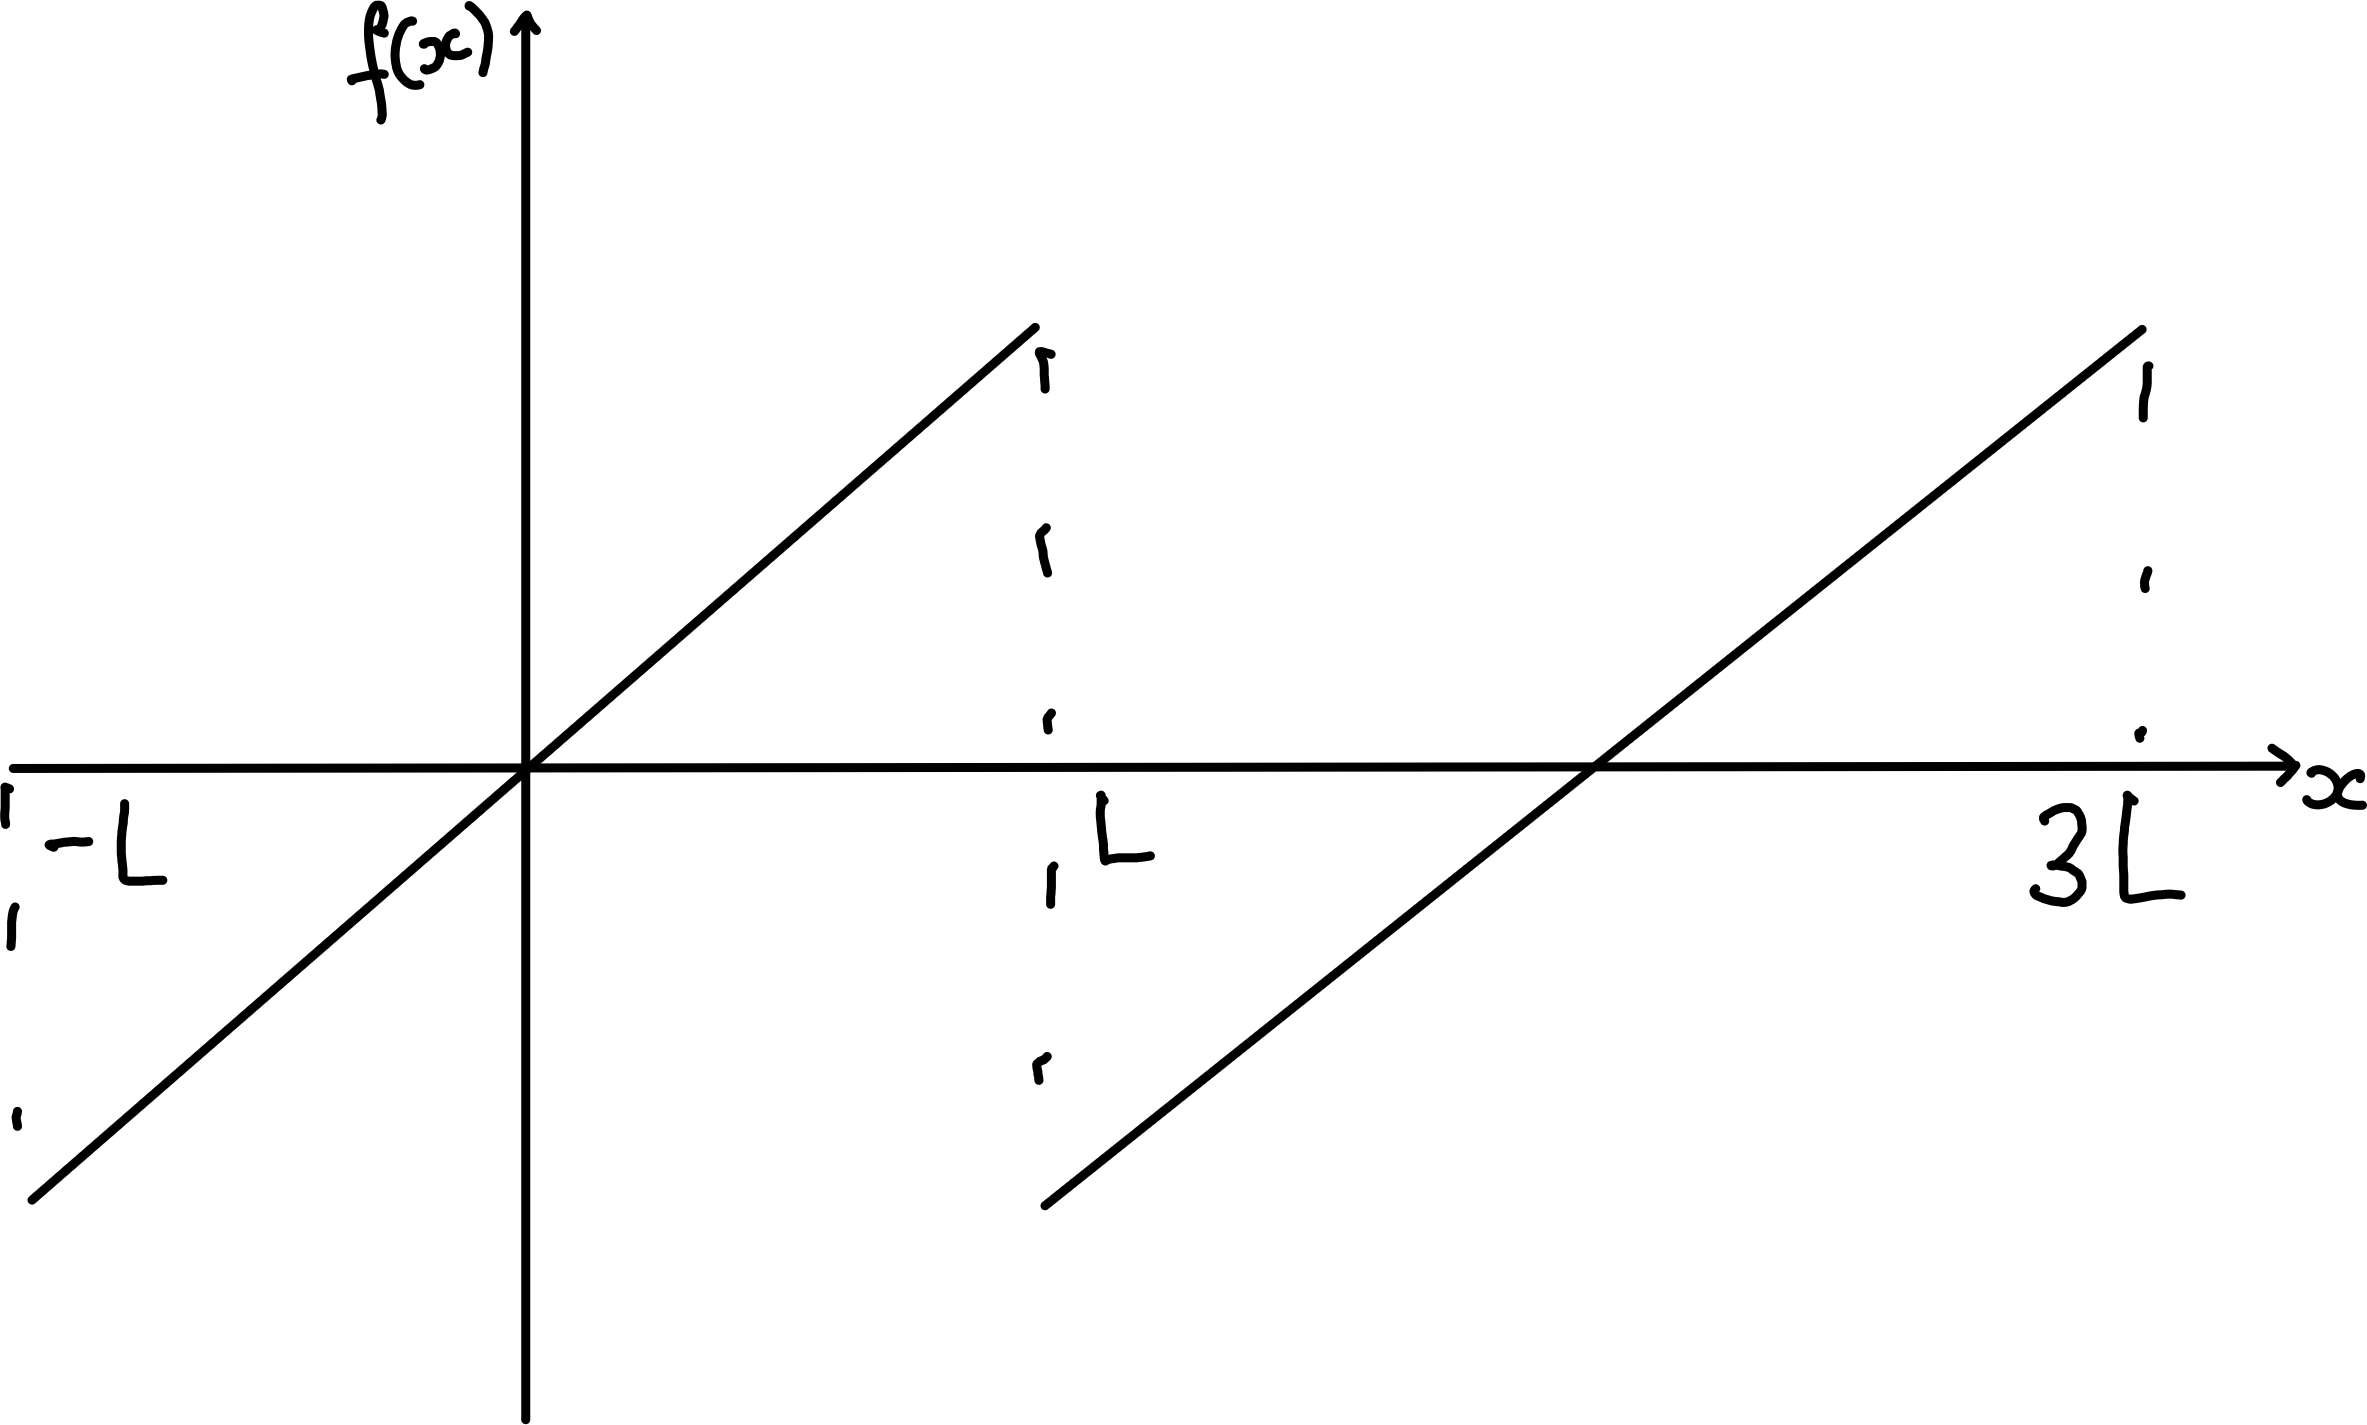
\includegraphics[height=5cm]{01-sawtooth} \par}
    Here,
    $a_n = \frac{1}{L} \int_{-L}^L x \cos \frac{n\pi x}{L} \dd{x} = 0$ as $x$ odd and $cos$ is even.
    \begin{align*}
        b_n &= \frac{1}{L} \int_{-L}^L x \sin \frac{n\pi x}{L} \dd{x} \\
        &= \frac{2}{L} \int_0^L x \sin \frac{n\pi x}{L} \dd{x} \text{ as the function we are integrating is even} \\
        &= \frac{-2}{n\pi} \qty[x \cos \frac{n\pi x}{L}]_0^L + \frac{2}{n\pi} \int_0^L \cos \frac{n \pi x}{L} \dd{x} \\
        &= \frac{-2L}{n\pi} \cos n \pi + \frac{2L}{(n\pi)^2} \sin n \pi \\
        &= \frac{2L}{n\pi} (-1)^{n+1}
    \end{align*}
    So the sawtooth FS is
    \begin{align} \label{eq:1.6}
        f(x) &= \frac{2L}{\pi} \sum_{n=1}^{\infty} \frac{(-1)^{n+1}}{n} \sin \frac{n \pi x}{L} \\
        &= \frac{2L}{\pi} \left( \sin \frac{\pi x}{L} - \frac{1}{2} \sin \frac{2 \pi x}{L} + \frac{1}{3} \sin \frac{3 \pi x}{L} + \dots \right) \notag
    \end{align} 
    which is slowly convergent.
    {\par \centering 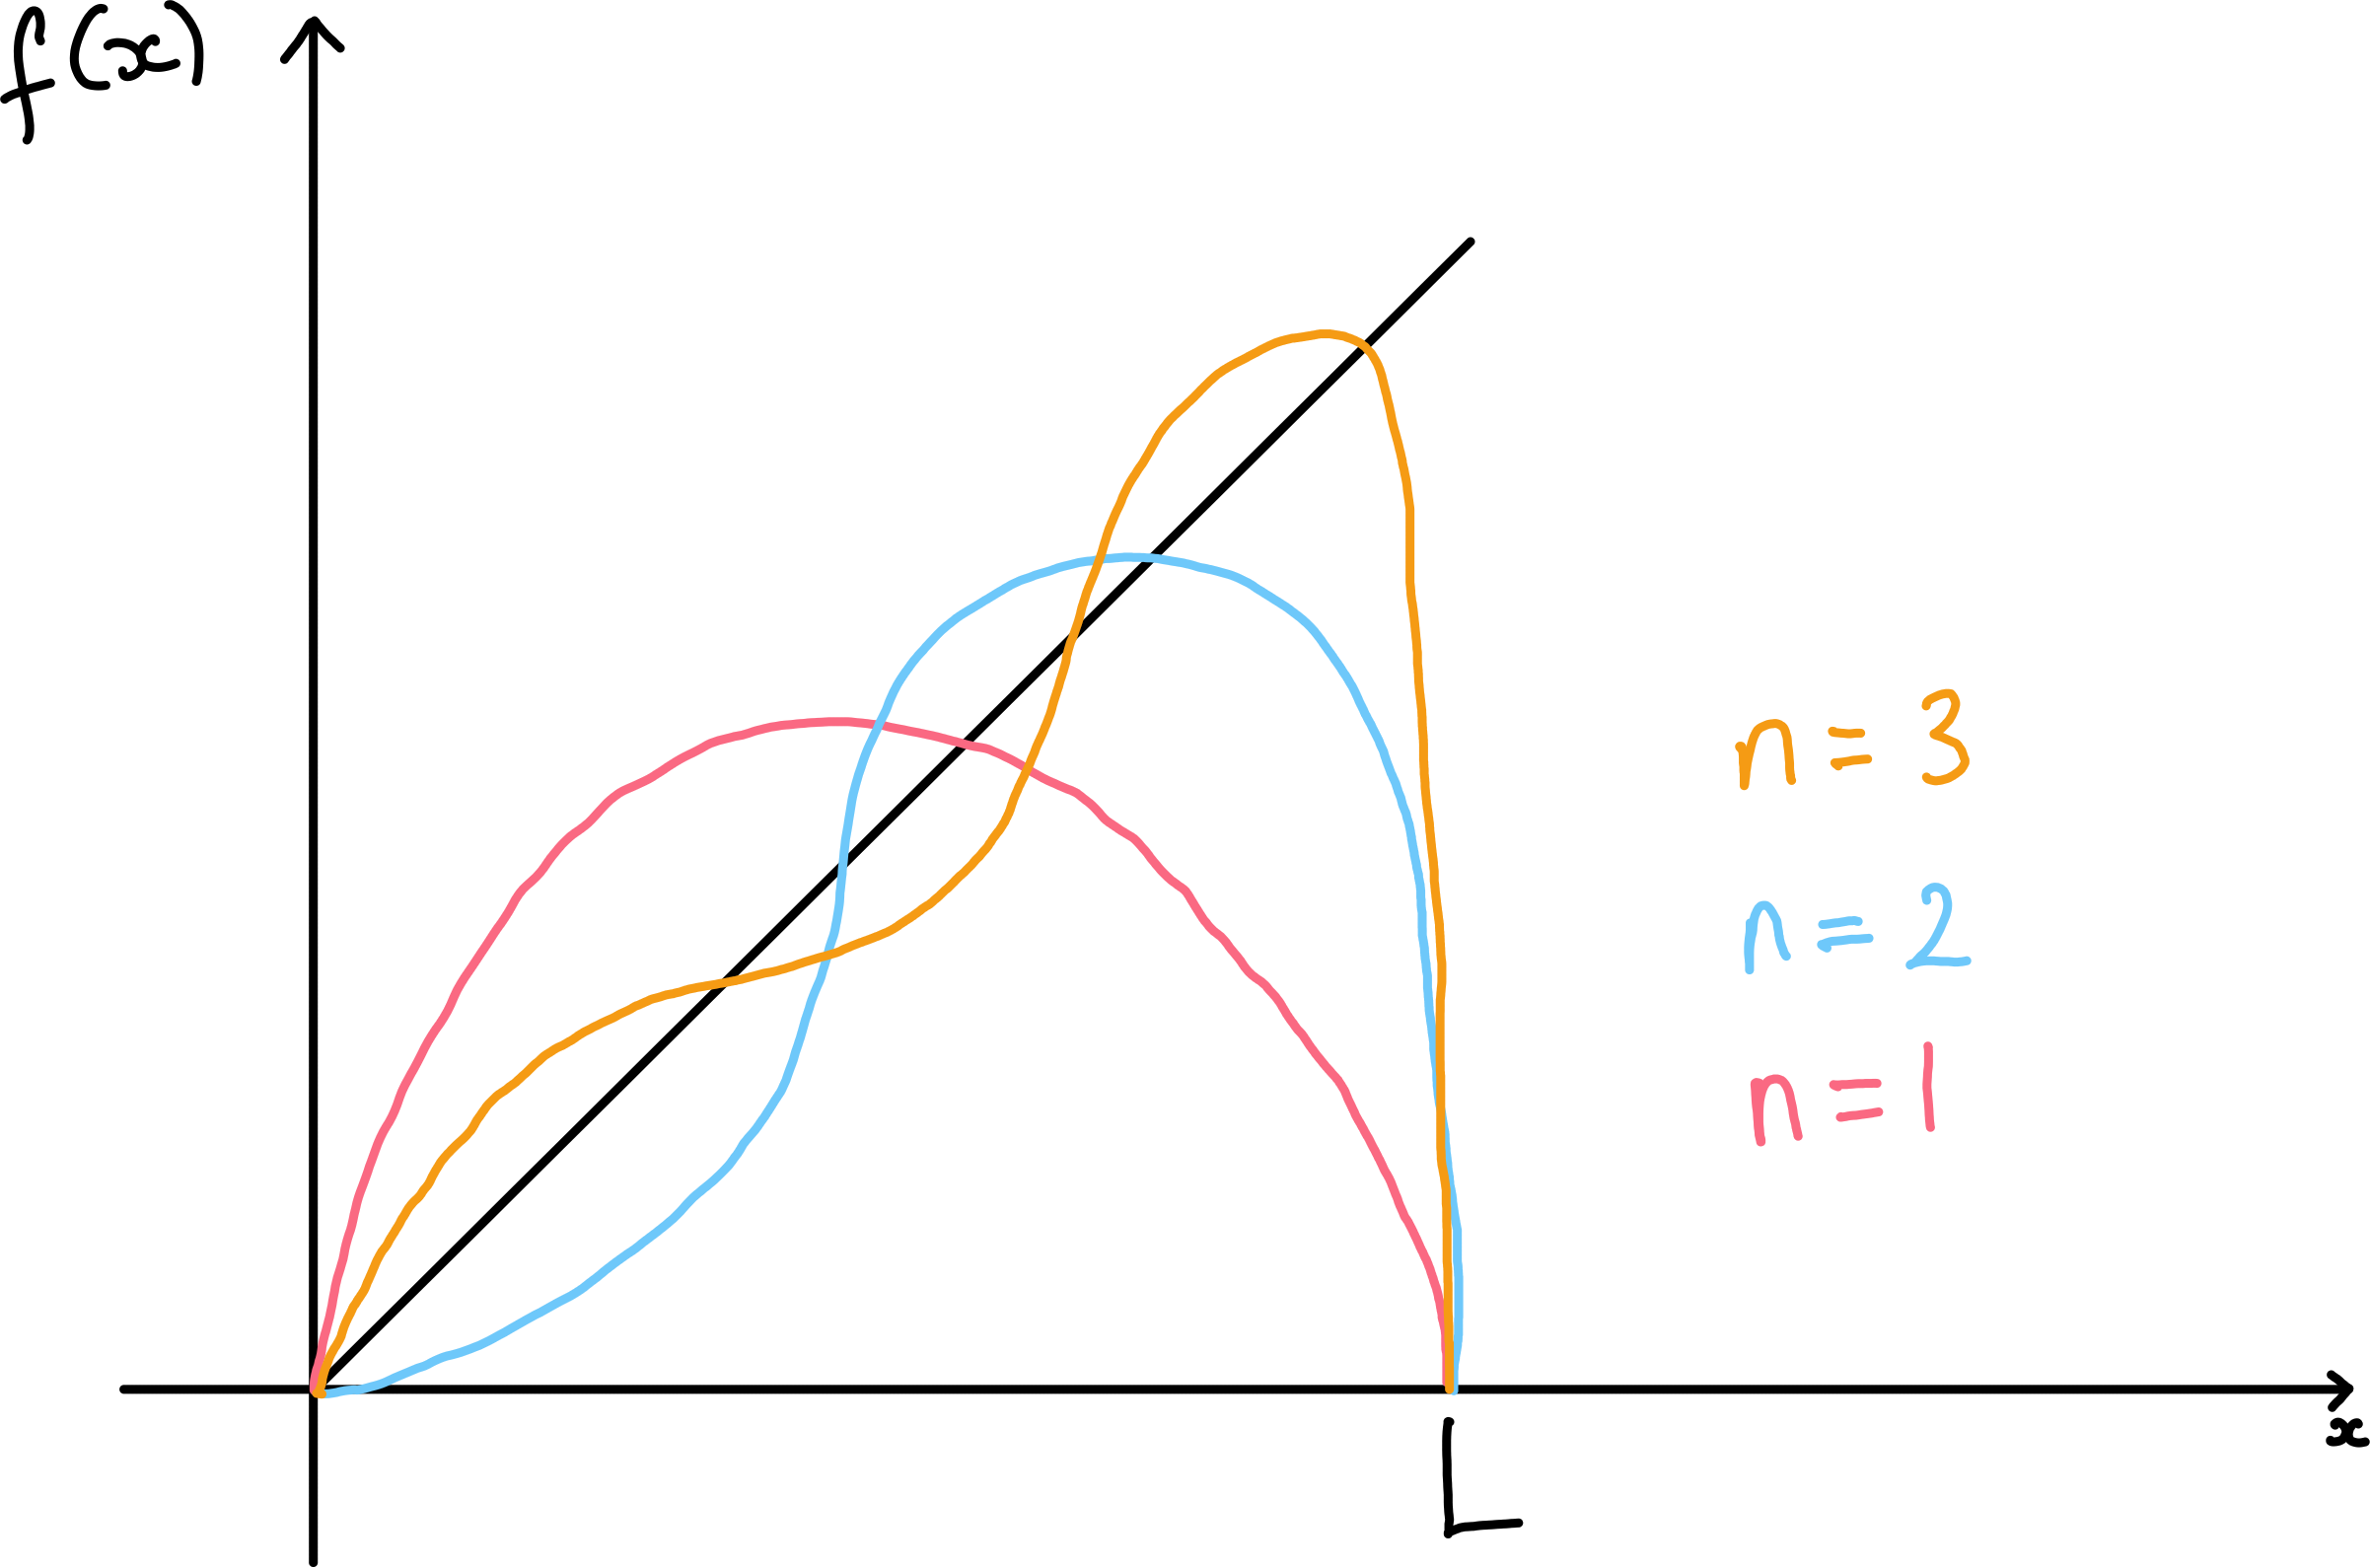
\includegraphics[height=5cm]{01-sawtooth2} \par}
\end{example}

\begin{note} As $n \to \infty$
    \begin{enumerate}
        \item FS approx improves (convergent when cts)
        \item $\text{FS} \to 0$ at $x = L$ i.e. midpoint of discontinuity
        \item FS has a persistent overshoot at $x = L$ (approx 9\% knows as Gibbs phenomenon, see Sheet 1, Q5).
    \end{enumerate} 
\end{note} 

\subsection{Dirichlet conditions}
The Dirichlet conditions are sufficiency conditions for a ``well-behaved'' function, that will imply the existence of a unique Fourier series.
\begin{theorem}
    If $f(x)$ is a bounded periodic function of period $2L$ with a finite number of minima, maxima and discontinuities in $[0, 2L)$, then the Fourier series converges to $f$ at all points at which $f$ is continuous, and at discontinuities the series converges to the midpoint.
\end{theorem}
\begin{note} \
    \begin{enumerate}
        \item These are some relatively weak conditions for convergence, compared to Taylor series.
            However, this definition still eliminates pathological functions such as $\frac{1}{x}$, $\sin \frac{1}{x}$, $\mathbbm 1 (\mathbb Q)$ and so on.
        \item \color{red}The converse is not true\color{black}; for example, $\sin \frac{1}{x}$ does in fact have a Fourier series.
        \item The proof is difficult and will not be given.
    \end{enumerate}
\end{note}

\noindent The rate of convergence of the Fourier series depends on the smoothness of the function.
\begin{theorem}
    If $f(x)$ has continuous derivatives up to a $p$th derivative which is discontinuous, then the Fourier series converges with order $O(n^{-(p+1)})$ as $n \to \infty$.
\end{theorem}
\begin{example}[$p = 0$]
    Consider the square wave (Sheet 1, Q5)
    \begin{align*}
        f(x) = \begin{cases}
            1  & 0 \leq x < 1  \\
            -1 & -1 \leq x < 0
        \end{cases}
    \end{align*}
    {\par \centering 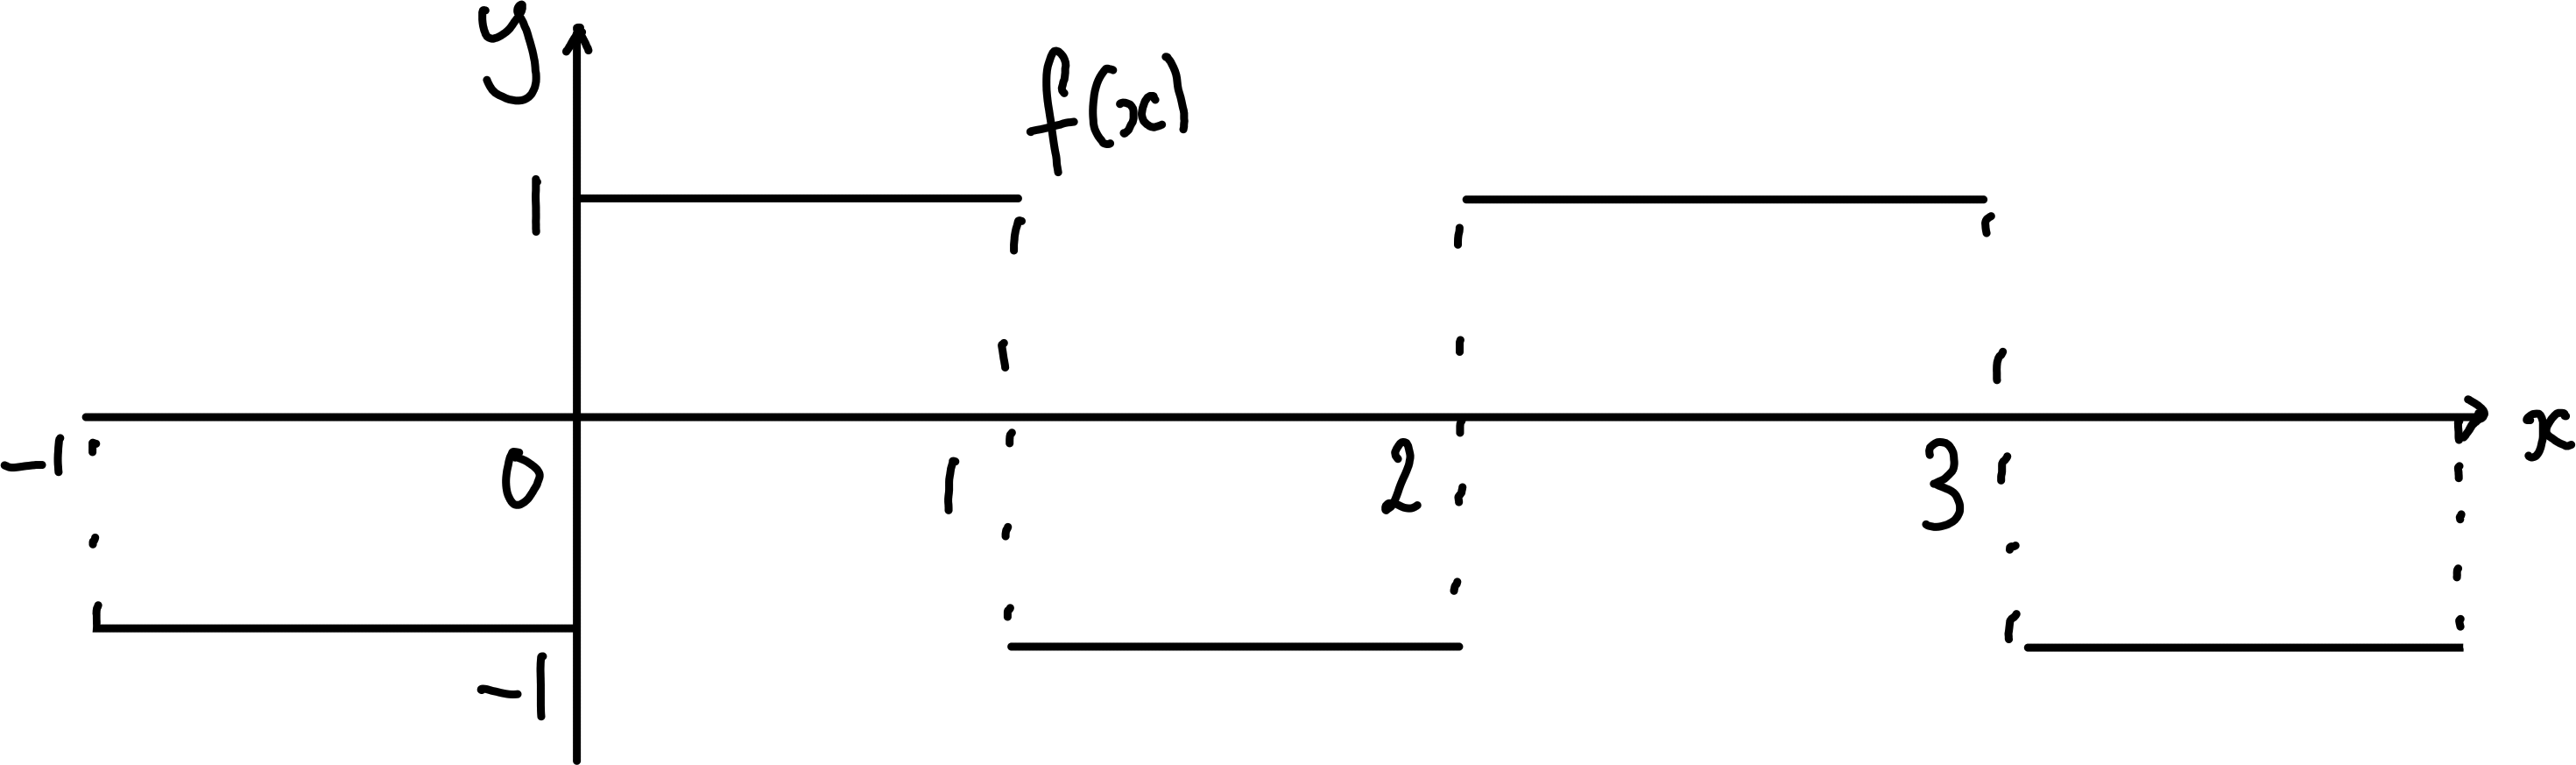
\includegraphics[height=5cm]{01-squarewave} \par}
    Then the Fourier series is
    \begin{align} \label{eq:1.7}
        f(x) = 4 \sum_{m=1}^\infty \frac{\sin (2m-1)\pi x}{(2m-1)\pi}
    \end{align}
\end{example}

\begin{example}[$p = 1$]
    Consider the general `see-saw' wave, defined by
    \begin{align*}
        f(x) = \begin{cases}
            x(1 - \xi) & 0 \leq x < \xi \\
            \xi(1 - x) & \xi \leq x < 1
        \end{cases}
    \end{align*}
    and defined as an odd function for $-1 \leq x < 0$.
    The Fourier series is\footnote{This is an important exercise you should do at home.}
    \begin{align} \label{eq:1.8}
        f(x) = 2 \sum_{m=1}^\infty \frac{\sin n\pi \xi \sin n\pi x}{(n \pi)^2}
    \end{align}
    
    {\par \centering 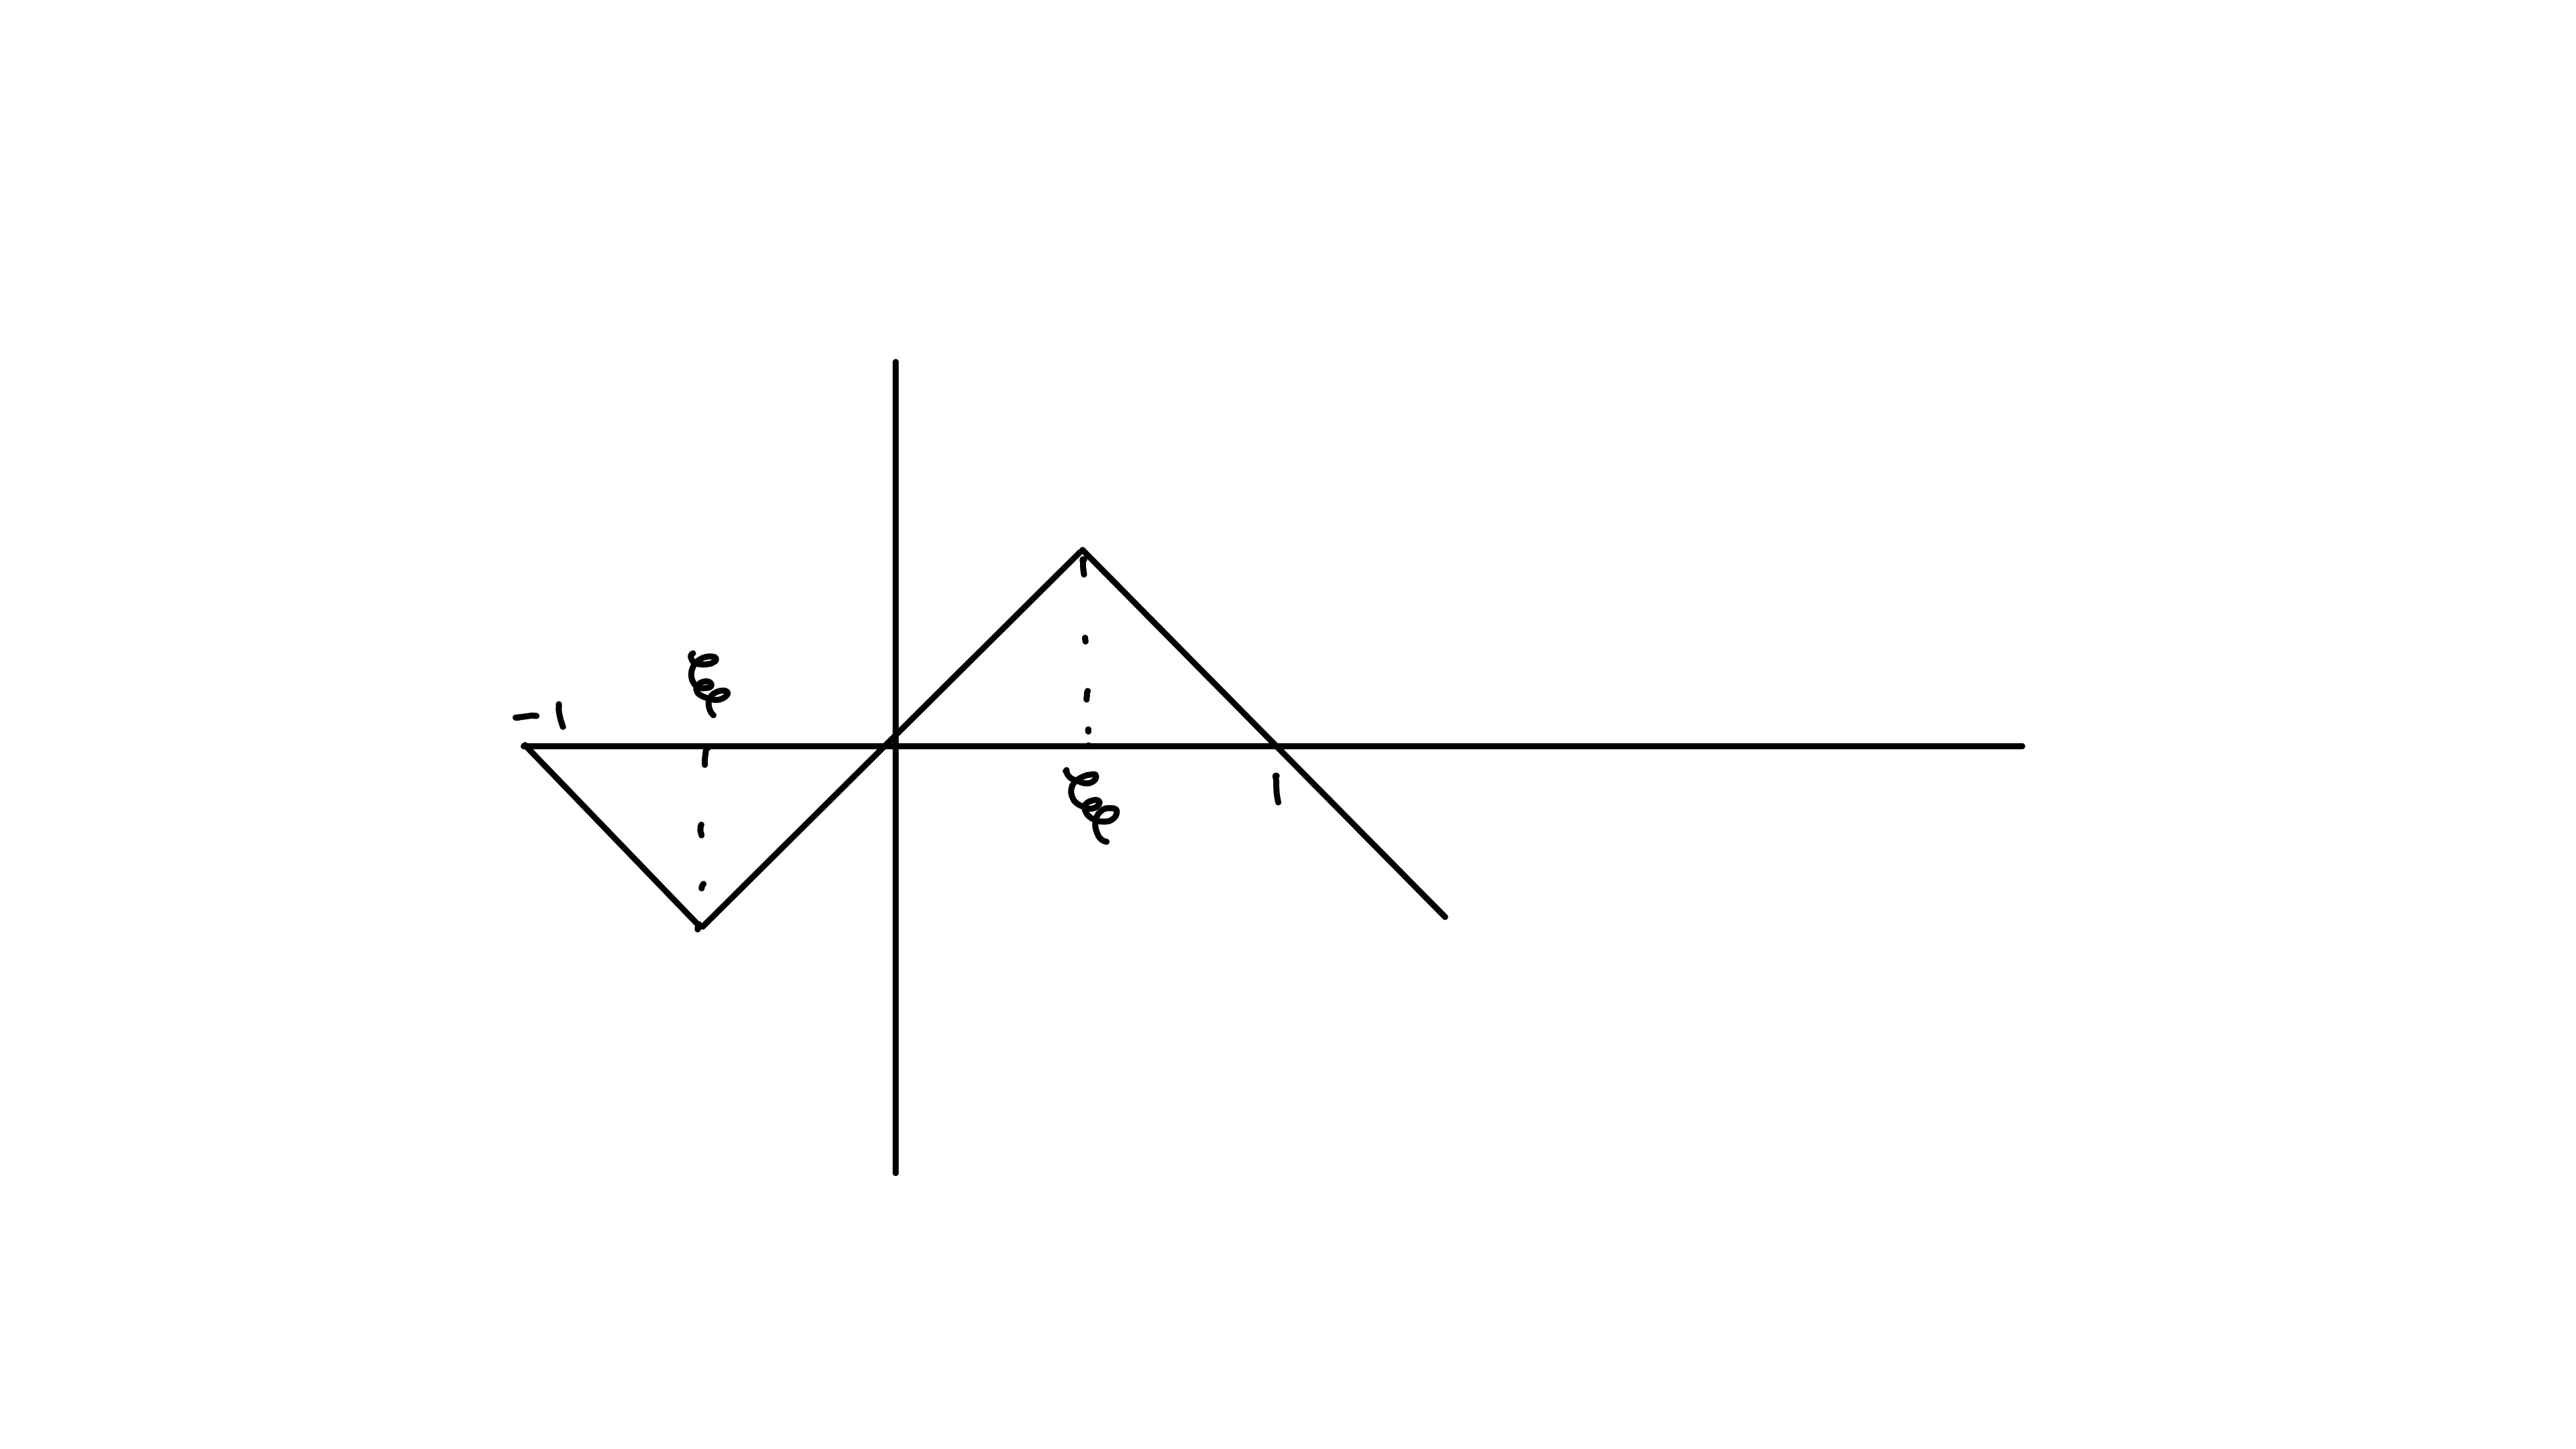
\includegraphics[height=5cm]{01-seesaw} \par}

    For instance, if $\xi = \frac{1}{2}$, we can show that
    \begin{align*}
        f(x) = 2 \sum_{m=1}^\infty (-1)^{m+1} \frac{\sin (2m-1)\pi x}{((2m-1)\pi)^2}
    \end{align*}
\end{example}
\begin{example}[$p = 2$]
    Let
    \begin{align*}
        f(x) = \frac{1}{2} x(1-x)
    \end{align*}
    for $0 \leq x < 1$, and defined as an odd function for $-1 \leq x < 0$.
    We can show that
    \begin{align} \label{eq:1.9}
        f(x) = 4\sum_{n=1}^\infty \frac{\sin(2m - 1)\pi x}{((2m-1)\pi)^3}
    \end{align}
    {\par \centering 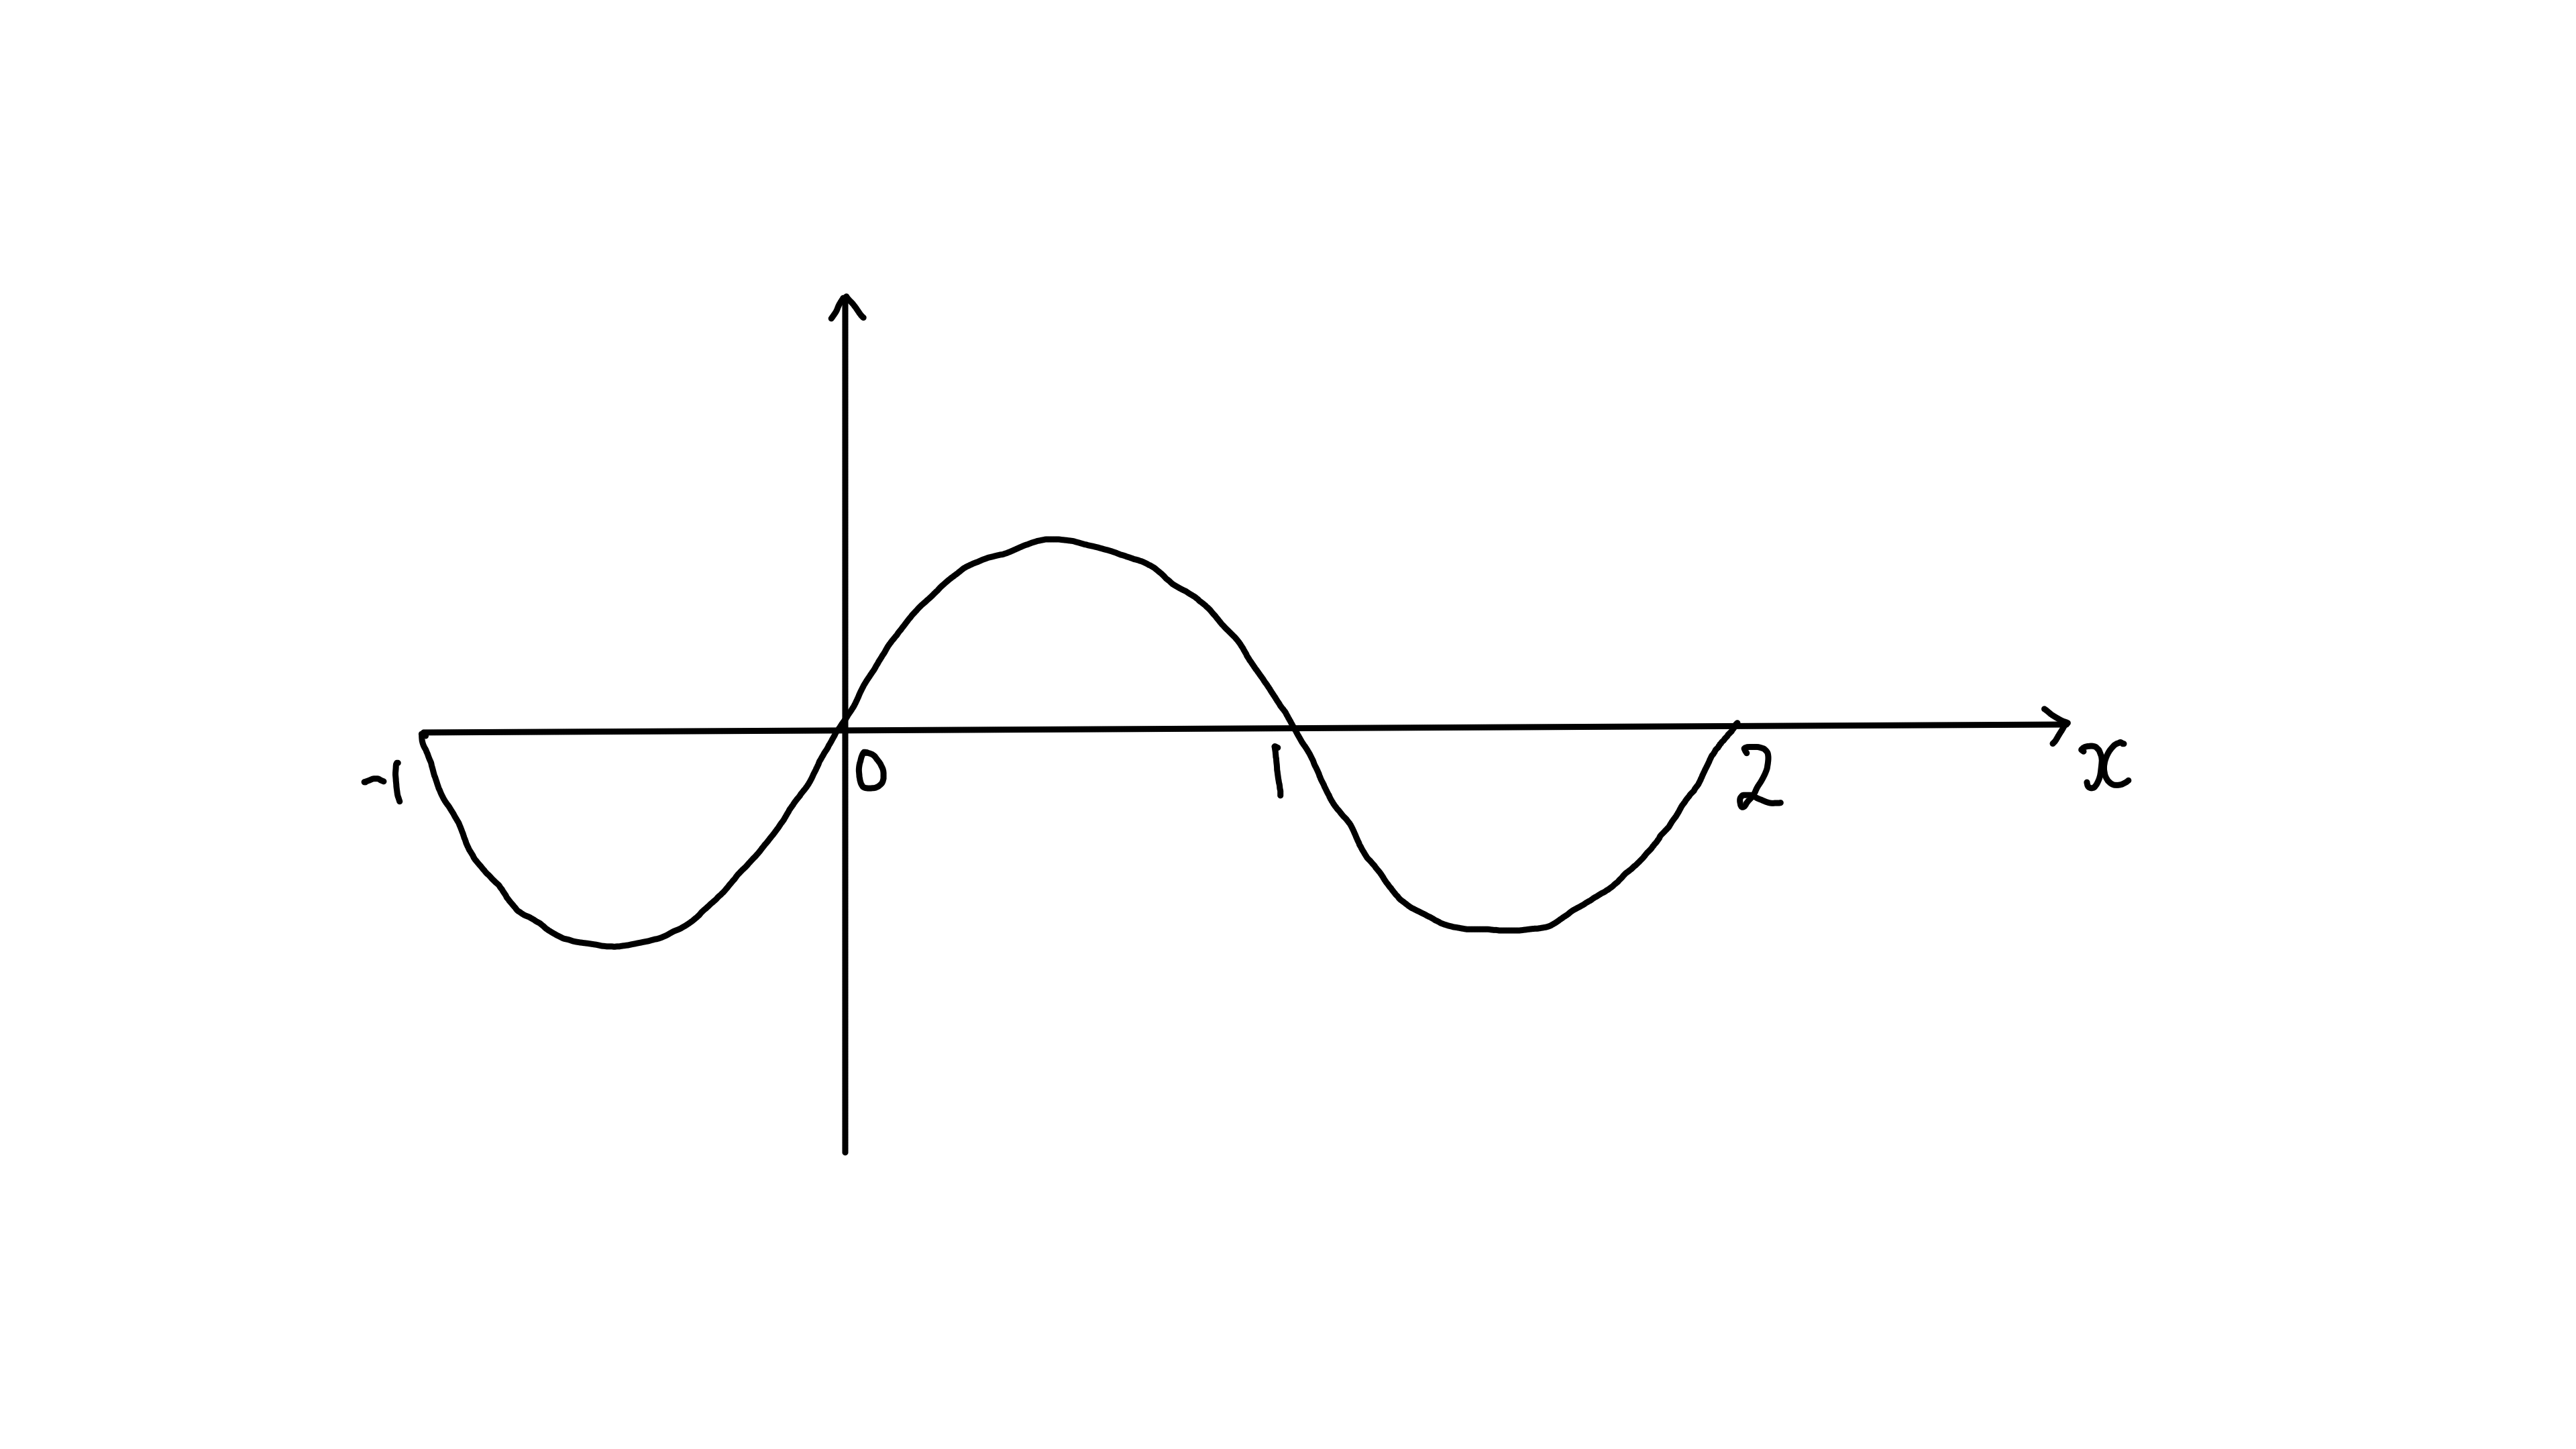
\includegraphics[height=5cm]{01-p2} \par}
\end{example}
\begin{example}[$p = 3$]
    Consider\footnote{Sheet 1, Q1}
    \begin{align*}
        f(x) = (1-x^2)^2
    \end{align*}
    with Fourier series
    \begin{align*}
        a_n = O\qty(\frac{1}{n^4})
    \end{align*}
\end{example}

\subsection{Integration of FS}
It is always valid to take the integral of a Fourier series term by term.
Defining $F(x) = \int_{-L}^x f(x) \dd{x}$, we can show that $F$ satisfies the Dirichlet conditions if $f$ does.
For instance, a jump discontinuity becomes continuous in the integral.

\subsection{Differentiation}
Differentiating term by term is not always valid.
For example, consider the square wave above:
\begin{align*}
    f(x) \stackrel{?}{=} 4 \sum_{m=1}^\infty \cos (2m-1)\pi x
\end{align*}
which is an unbounded series (consider $x = 0$).
\begin{theorem}
    If $f(x)$ is continuous and satisfies the Dirichlet conditions, and $f'(x)$ also satisfies the Dirichlet conditions, then $f'(x)$ can be found term by term by differentiating the Fourier series of $f(x)$.
\end{theorem}
\begin{example}
    We can differentiate the see-saw function, \cref{eq:1.8}, with $\xi = \frac{1}{2}$, even though the derivative is not continuous.
    The result is an offset square wave, or by mapping $x \mapsto x + \frac{1}{2}$ we recover the original square wave, \cref{eq:1.7}.
\end{example}

\subsection{Parseval's theorem}
Parseval's theorem relates the integral of the square of a function with the sum of the squares of the function's Fourier series coefficients.
\begin{theorem}[Parseval's theorem]
    Suppose $f$ has Fourier coefficients $a_i, b_i$.
    Then
    \begin{align}
        \int_0^{2L} [f(x)]^2 \dd{x} & = \int_0^{2L} \qty[ \frac{1}{2}a_0 + \sum_{n=1}^\infty a_n \cos \frac{n \pi x}{L} + \sum_{n=1}^\infty b_n \sin \frac{n\pi x}{L} ]^2 \dd{x} \notag \\
        \intertext{We can remove cross terms, since the basis functions are orthogonal. \cref{eq:1.1,eq:1.2,eq:1.3}}
        & = \int_0^{2L} \qty[ \frac{1}{4} a_0^2 + \sum_{n=1}^\infty a_n^2 \cos^2 \frac{n\pi x}{L} + \sum_{n=1}^\infty b_n^2 \sin^2 \frac{n\pi x}{L} ] \dd{x} \notag \\
        & = L \qty[ \frac{1}{2} a_0^2 + \sum_{n=1}^\infty (a_n^2 + b_n^2) ] \label{eq:1.10}
    \end{align}
\end{theorem}
\noindent This is also called the \textit{completeness relation}: the left hand side is greater than or equal to the right hand side if any of the basis functions are missing.
\begin{example}
    Let us apply Parseval's theorem to the sawtooth wave with FS \cref{eq:1.6}.
    \begin{align*}
        \int_{-L}^L [f(x)]^2 \dd{x} = \int_{-L}^L x^2 \dd{x} = \frac{2}{3}L^3
    \end{align*}
    The right hand side gives
    \begin{align*}
        L \sum_{n=1}^\infty \frac{4L^2}{n^2 \pi^2} = \frac{4 L^3}{\pi^2} \sum_{n=1}^\infty \frac{1}{n^2}
    \end{align*}
    Parseval's theorem then implies\footnote{Sheet 1, Q3}
    \begin{align*}
        \sum_{n=1}^\infty \frac{1}{n^2} = \frac{\pi^2}{6}
    \end{align*}
\end{example}
\begin{note}
    Parseval's theorem for functions $\inner{f, f} = \norm{f}^2$ is equivalent to Pythagoras for vectors $\inner{v, v} = \norm{v}^2$.
\end{note} 

\subsection{Half-range series}
Consider $f(x)$ defined only on $0 \leq x < L$.
We can extend the range of $f$ to be the full range $-L \leq x < L$ in two simple ways:
\begin{enumerate}
    \item require $f$ to be odd, so $f(-x) = -f(x)$.
        Hence, $a_n = 0$ (as $\cos$ is even) and
        \begin{align} \label{eq:1.11}
            b_n = \frac{2}{L} \int_0^L f(x) \sin \frac{n \pi x}{L} \dd{x}
        \end{align}
        So
        \begin{align*}
            f(x) = \sum_{n=1}^\infty b_n \sin \frac{n\pi x}{L}
        \end{align*}
        which is called a Fourier sine series.
    \item require $f$ to be even, so $f(-x) = f(x)$.
        In this case, $b_n = 0$ and
        \begin{align} \label{eq:1.12}
            a_n = \frac{2}{L} \int_0^L f(x) \cos \frac{n \pi x}{L} \dd{x}
        \end{align}
        and so
        \begin{align*}
            f(x) = \frac{1}{2}a_0 + \sum_{n=1}^\infty a_n \cos \frac{n\pi x}{L}
        \end{align*}
        which is a Fourier cosine series.
\end{enumerate}

\subsection{Complex representation of Fourier series}
Recall that
\begin{align*}
    \cos \frac{n \pi x}{L} &= \frac{1}{2}\qty(e^{i n \pi x / L} + e^{-i n \pi x / L}); \\
    \sin \frac{n \pi x}{L} &= \frac{1}{2i}\qty(e^{i n \pi x / L} - e^{-i n \pi x / L})
\end{align*}
Therefore, a Fourier series can be written as
\begin{align}
    f(x) &= \frac{1}{2} a_0 + \frac{1}{2} \sum_{n=1}^\infty \qty[ (a_n - i b_n) e^{i n \pi x / L} + (a_n + i b_n) e^{-i n \pi x / L} ] \notag \\
    &= \sum_{m=-\infty}^\infty c_m e^{i m \pi x / L} \label{eq:1.13}
\end{align}
where for $m > 0$ we have $m=n, c_m = \frac{1}{2}(a_n - ib_n)$, and for $m < 0$ we have $n = -m, c_m = \frac{1}{2}(a_{-m} + ib_{-m})$, and where $m = 0$ we have $c_0 = \frac{1}{2} a_0$.
In particular,
\begin{align} \label{eq:1.14}
    c_m = \frac{1}{2L} \int_{-L}^L f(x) e^{-i m \pi x / L} \dd{x}
\end{align}
where the negative sign comes from the complex conjugate.
This is because, for complex-valued $f, g$, we have
\begin{definition}[Complex inner product] ~\vspace*{-1.5\baselineskip}
    \begin{align*}
        \inner{f,g} = \int_{-L}^L f^\star\footnote{$f^\star$ is the complex conjugate of $f$.} g \dd{x}
    \end{align*}
\end{definition} 
The orthogonality conditions are
\begin{align} \label{eq:1.15}
    \int_{-L}^L e^{-i m \pi x / L} e^{i n \pi x / L} \dd{x} = 2L \delta_{mn}
\end{align}
Parseval's theorem now states
\begin{align*}
    \int_{-L}^L f^\star(x) f(x) \dd{x} = \int_{-L}^L \abs{f(x)}^2 \dd{x} = 2L \sum_{m=-\infty}^\infty \abs{c_m}^2
\end{align*}

\subsection{Self-adjoint matrices}
\textit{Much of this section is a recap of IA Vectors and Matrices.}
Suppose that $u, v \in \mathbb C^N$ with inner product
\begin{align} \label{eq:1.16}
    \inner{u,v} = u^\dagger v
\end{align}
\begin{definition}[Hermitian matrix] 
    The $N \times N$ matrix $A$ is \textit{self-adjoint}, or \textit{Hermitian}, if
    \begin{align*}
        \forall u,v \in \mathbb C^N, \inner{Au, v} = \inner{u, Av} \iff A^\dagger = A
    \end{align*}
\end{definition} 
The eigenvalues $\lambda_n$ and eigenvectors $v_n$ satisfy
\begin{align} \label{eq:1.17}
    A v_n = \lambda_n v_n
\end{align}
They have the following properties:
\begin{enumerate}
    \item $\lambda_n^\star = \lambda_n$;
    \item $\lambda_n \neq \lambda_m \implies \inner{ v_n, v_m } = 0$;
    \item we can create an orthonormal basis from the eigenvectors.
\end{enumerate}
Given $b \in \mathbb C^n$, we can solve for $x$ in the general matrix equation 
\begin{align}
    Ax = b \label{eq:1.18}
\end{align}
Express $b$ in terms of the eigenvector basis:
\begin{align*}
    b = \sum_{n=1}^N b_n v_n \notag
\end{align*}
We seek a solution of the form
\begin{align*}
    x = \sum_{n=1}^N c_n v_n
\end{align*}
At this point, the $b_n$ are known and the $c_n$ are our target.
Substituting into the matrix equation \cref{eq:1.18}, orthogonality of basis vectors gives
\begin{align*}
    A \sum_{n=1}^N c_n v_n &= \sum_{n=1}^N b_n v_n \\
    \sum_{n=1}^N c_n \lambda_n v_n &= \sum_{n=1}^N b_n v_n
    \intertext{As the eigenvector basis is orthogonal we can equate coefficients}
    c_n \lambda_n &= b_n \\
    c_n &= \frac{b_n}{\lambda_n}
\end{align*}
Therefore,
\begin{align} \label{eq:1.19}
    x = \sum_{n=1}^N \frac{b_n}{\lambda_n} v_n
\end{align}
provided $\lambda_n \neq 0$, or equivalently, the matrix is invertible.

\subsection{Solving inhomogeneous ODEs with Fourier series} \label{sec:1.6}
We wish to find $y(x)$ given a driving/ source term $f(x)$ for the general differential equation
\begin{align} \label{eq:1.20}
    \mathcal L y \equiv -\dv[2]{y}{x} = f(x)
\end{align}
with boundary conditions $y(0) = y(L) = 0$.
The related eigenvalue problem is
\begin{align*}
    \mathcal L y_n = \lambda_n y_n,\quad y_n(0) = y_n(L) = 0
\end{align*}
which has solutions
\begin{align} \label{eq:1.21}
    y_n(x) = \sin \frac{n \pi x}{L},\ \lambda_n = \qty(\frac{n\pi}{L})^2
\end{align}
We can show that this is a self-adjoint linear operator\footnote{https://math.stackexchange.com/questions/4356100/why-is-the-second-derivative-operator-self-adjoint} with orthogonal eigenfunctions.
We seek solutions of the form of a half-range sine series.
Consider
\begin{align*}
    y(x) = \sum_{n=1}^\infty c_n \sin\frac{n \pi x}{L}
\end{align*}
The right hand side is
\begin{align*}
    f(x) = \sum_{n=1}^\infty b_n \sin \frac{n \pi x}{L}
\end{align*}
We can find $b_n$ by
\begin{align*}
    b_n = \frac{2}{L} \int_0^L f(x) \sin \frac{n \pi x}{L} \dd{x}
\end{align*}
Substituting into \cref{eq:1.20}, we have
\begin{align*}
    \mathcal L y = -\dv[2]{x} \qty(\sum_n c_n \sin \frac{n \pi x}{L}) &= \sum_n c_n \qty(\frac{n\pi}{L})^2 \sin \frac{n \pi x}{L} \\
    \text{So } \sum_n c_n \qty(\frac{n\pi}{L})^2 \sin \frac{n \pi x}{L} &= \sum_n b_n \sin \frac{n \pi x}{L}
\end{align*}
By orthogonality \cref{eq:1.1},
\begin{align*}
    c_n \qty(\frac{n \pi}{L})^2 = b_n \implies c_n = \qty(\frac{L}{n \pi})^2 b_n
\end{align*}
Therefore the solution is
\begin{align} \label{eq:1.22}
    y(x) = \sum_n \qty(\frac{L}{n \pi})^2 b_n \sin \frac{n \pi x}{L} = \sum_n \frac{b_n}{\lambda_n} y_n
\end{align}
which is equivalent to the solution we found for self-adjoint matrices for which the eigenvalues and eigenvectors are known.
\begin{example}[Odd square wave]
    Consider an odd square wave with $L = 1$, so $f(x) = 1$ from $0 \leq x < 1$.
    \begin{align*}
        f(x) = 4 \sum_m \frac{\sin(2m-1)\pi x}{(2m-1)\pi} \text{ by \cref{eq:1.7}}
    \end{align*}
    Then the solution to $\mathcal L y = f$ \cref{eq:1.22} should be (with odd $n = 2m-1$)
    \begin{align*}
        y(x) = \sum_n \frac{b_n}{\lambda_n} y_n = 4 \sum_n \frac{\sin (2m-1) \pi x}{((2m - 1) \pi)^3}
    \end{align*}
    This is exactly the Fourier series for
    \begin{align*}
        y(x) = \frac{1}{2}x(1-x) \text{ by \cref{eq:1.9}}
    \end{align*}
    so this $y$ is the solution to the differential equation.
    We can in fact integrate $\mathcal L y = 1$ directly with the boundary conditions to verify the solution.
    We can also differentiate the Fourier series for $y$ twice to find the square wave.
\end{example}
    \section{Sturm-Liouville Theory}

\subsection{Review of second-order linear ODEs}
\textit{This section is a review of IA Differential Equations.}

We wish to solve a general inhomogeneous ODE, written
\begin{align} \label{eq:2.1}
    \mathcal L y \equiv \alpha(x) y'' + \beta(x) y' + \gamma(x) y = f(x)
\end{align}
The homogeneous version has $f(x) = 0$, so \begin{align} \label{eq:2.2}
    \mathcal{L}y = 0,
\end{align} which has two independent solutions $y_1, y_2$.
The general solution, also the complementary function for the inhomogeneous ODE, is 
\begin{align}
    y_c(x) = A y_1(x) + B y_2(x). \label{eq:2.3}
\end{align}

The inhomogeneous equation 
\begin{align}
    \mathcal L y = f(x) \label{eq:2.4}
\end{align} has a solution called the particular integral, denoted $y_p(x)$.
The general solution to this equation is then 
\begin{align} \label{eq:2.5}
    y(x) = y_p + y_c.
\end{align}

We need two boundary or initial conditions to find the particular solution to the differential equation.
Suppose $x \in [a,b]$.
We can create boundary conditions by defining $y(a), y(b)$, often called the Dirichlet conditions.
Alternatively, we can consider $y(a), y'(a)$, called the Neumann conditions.
We could also used some kind of mixed condition, for instance $y + ky'$.

Homogeneous boundary conditions are such that $y(a) = y(b) = 0$.
In this part of the course, homogeneous boundary conditions are often assumed.
Note that we can add a complementary function $y_c$ to the solution, for instance $\overline{y} = y + A y_1 + B y_2$ such that $\overline{y}(a) = \overline{y}(b) = 0$.
This would allow us to construct homogeneous boundary conditions even when they are not present \textit{a priori} in the problem.
We could also specify initial data, such as solving for $x \geq a$, given $y, y'$ at $x = a$.

To solve the inhomogeneous equation \cref{eq:2.1}, we want to use eigenfunction expansions (like FS \cref{eq:1.22}).
In order to do this, we must first solve the \underline{related} eigenvalue problem.
In this case, that is
\begin{align}
    \alpha(x) y'' + \beta(x) y' + \gamma(x) y = -\lambda \rho(x) y. \label{eq:2.6}
\end{align}
We must solve this equation with the same boundary conditions as the original problem.
This form of equation often arises as a result of applying a separation of variables, particularly for PDEs in several dimensions.

\subsection{Sturm-Liouville form}
\begin{definition}[Inner product]
    For two complex-valued functions $f, g$ on $[a,b]$, we define the inner product as
    \begin{align*}
        \inner{f,g} = \int_a^b f^\star(x) g(x) \dd{x}
    \end{align*} 
\end{definition} 
The eigenvalue problem \cref{eq:2.6} above greatly simplifies if $\mathcal L$ is \underline{self-adjoint}, that is, if it can be expressed in \underline{Sturm-Liouville form}:
\begin{align} \label{eq:2.7}
    \mathcal L y \equiv -(py')' + qy = \lambda w y.
\end{align}
$\lambda$ is an eigenvalue, and $w(x)$ is the \textit{weight function}, which must be non-negative $w(x) \geq 0 \ \forall \; x$.

\subsection{Converting to Sturm-Liouville form}
Multiply \cref{eq:2.6} by an integrating factor $F(x)$ to give
\begin{align*}
    F \alpha y'' + F \beta y' + F \gamma y &= -\lambda F \rho y \\
    \dv{x} \qty(F \alpha y') - F' \alpha y' - F \alpha' y' + F \beta y' + F \gamma y &= -\lambda F \rho y
\end{align*}
To eliminate the $y'$ term, we require $F'\alpha = F(\beta - \alpha')$.
Thus,
\begin{align}
    \frac{F'}{F} &= \frac{\beta - \alpha'}{\alpha} \notag \\
    \implies F &= \exp \int^x \frac{\beta - \alpha'}{\alpha} \dd{x} \label{eq:2.8}
\end{align}
and further,
\begin{align*}
    (F\alpha y')' + F \gamma y = - \lambda F \rho y
\end{align*}
hence
\begin{align*}
    p & = F \alpha \\
    q & = F \gamma \\
    w & = F \rho
\end{align*} in $\cref{eq:2.7}$ and $F(x) > 0$ hence $w > 0$.
\begin{example}
    Consider the Hermite equation for simple harmonic oscillator,
    \begin{align*}
        y'' - 2xy' + 2ny = 0
    \end{align*}
    In this case for \cref{eq:2.6} $\alpha = 1,\ \beta = -2x,\ \gamma = 0,\ \lambda p = 2n$.
    So by \cref{eq:2.8}
    \begin{align*}
        F = \exp \int^x \frac{-2x}{1} \dd{x} = e^{-x^2}
    \end{align*}
    Then the equation, in Sturm-Liouville form, is
    \begin{align}
        \mathcal L y \equiv -\qty(e^{-x^2} y')' = 2n e^{-x^2} y \label{eq:2.9}
    \end{align}
\end{example}

\subsection{Self-adjoint operators}
\begin{definition}[Self-adjoint operator]
    $\mathcal L$ is a self-adjoint operator on $[a,b]$ for all pairs of functions $y_1,y_2$ satisfying appropriate boundary conditions if
    \begin{align*}
        \inner{y_1, \mathcal L y_2} = \inner{\mathcal L y_1, y_2}
    \end{align*}
\end{definition}
Written explicitly,
\begin{align} \label{eq:2.10}
    \int_a^b y_1^\star(x) \mathcal L y_2(x) \dd{x} = \int_a^b (\mathcal L y_1(x))^\star y_2(x) \dd{x}
\end{align}

\underline{Boundary conditions}: Substituting Sturm-Liouville form \cref{eq:2.7} into the above,
\begin{align}
    \inner{y_1, \mathcal L y_2} - \inner{\mathcal L y_1, y_2} &= \int_a^b \qty[-y_1 (py_2')' + y_1 q y_2 + y_2 (p y_1')' - y_2 q y_1] \dd{x} \notag \\
    &= \int_a^b \qty[-y_1 (py_2')' + y_2 (p y_1')'] \dd{x} \notag
    \intertext{Adding $-y_1' p y_2' + y_1' p y_2'$,}
    &= \int_a^b \qty[-(py_1y_2')' + (py_1'y_2)'] \dd{x} \notag \\
    &= [-py_1y_2' + py_1'y_2]_a^b \label{eq:2.11}
\end{align}
which must be zero for an equation in Sturm-Liouville form to be self-adjoint.

\subsection{Self-adjoint compatible boundary conditions}
\begin{itemize}
    \item Suppose $y(a) = y(b) = 0$.
        Then certainly the Sturm-Liouville form of the differential equation is self-adjoint.
        We could also choose $y'(a) = y'(b) = 0$ or $y + ky' = 0$.
        Collectively, the act of using homogeneous boundary conditions is known as the \textit{regular} Sturm-Liouville problem.
    \item Periodic boundary conditions could also be used, such as $y(a) = y(b)$.
    \item If $a$ and $b$ are singular points of the equation, i.e.
        $p(a) = p(b) = 0$, this is self-adjoint compatible.
    \item We could also have combinations of the above properties, one at $a$ and one at $b$.
\end{itemize}

\subsection{Properties of self-adjoint operators}
The following properties hold for any self-adjoint differential operator $\mathcal L$.
\begin{enumerate}
    \item The eigenvalues $\lambda_n$ are real (also eigenfunctions are real).
    \item The eigenfunctions $y_n$ are orthogonal.
    \item The $y_n$ are a complete set; they span the space of all functions hence our general solution can be written in terms of these eigenfunctions.
\end{enumerate}
Each property is proven in its own subsection.

\subsection{Real eigenvalues}
\begin{proof}
    Suppose we have some eigenvalue $\lambda_n$, so
    \begin{align} \label{eq:2.12}
        \mathcal L y_n = \lambda_n w y_n.
    \end{align} 
    Taking the complex conjugate, $\mathcal L y_n^\star = \lambda_n^\star w y_n^\star$, since $\mathcal L, w$ are real.
    Now, consider
    \begin{align*}
        \int_a^b \qty(y_n^\star \mathcal L y_n - y_n \mathcal L y_n^\star) \dd{x}
    \end{align*}
    which must be zero if $\mathcal L$ is self-adjoint, \cref{eq:2.10}.
    This can be written as
    \begin{align*}
        (\lambda_n - \lambda_n^\star) \int_a^b w y_n^\star y_n \dd{x} = 0
    \end{align*}
    The integral is nonzero, hence $\lambda_n - \lambda_n^\star = 0$ which implies $\lambda_n$ is real.
\end{proof}

\begin{aside}{Aside}
    Note, if the $\lambda_n$ are non-degenerate (simple), i.e.\ with a unique eigenfunction $y_n$, then $y_n^\star = y_n$ hence they are real.
    We can in fact show that (for a second-order equation) it is always possible to take linear combinations of eigenfunctions such that the result is linear, for example in the exponential form of the Fourier series.
    Hence, we can assume that $y_n$ is real.

    We can further prove that the regular Sturm-Liouville problem must have simple (non-degenerate) eigenvalues $\lambda_n$, by considering two possible eigenfunctions $u, v$ for the same $\lambda$, and use the expression for self-adjointness.
    We find $u \mathcal L v - (\mathcal L u) v = [-p(uv' - u'v)]'$ which contains the Wronskian.
    We can integrate and impose homogeneous boundary conditions to get the required result.
\end{aside} 

\subsection{Orthogonality of eigenfunctions}
Suppose $\mathcal L y_n = \lambda_n w y_n$ \cref{eq:2.12}, and $\mathcal L y_m = \lambda_m w y_m$ where $\lambda_n \neq \lambda_m$.
Then, we can integrate to find
\begin{align*}
    \int_a^b (y_m \mathcal L y_n - y_n \mathcal L y_m) \dd{x} = (\lambda_n - \lambda_m) \int_a^b w y_n y_m \dd{x} = 0 \text{ by self-adjointness \cref{eq:2.10}}
\end{align*}
Since $\lambda_n \neq \lambda_m$, we have
\begin{align} \label{eq:2.13}
    \forall n \neq m, \int_a^b w y_n y_m \dd{x} = 0
\end{align}
Hence, $y_n$ and $y_m$ are orthogonal \textit{with respect to} the weight function $w$ on $[a,b]$.
\begin{definition}[Inner product]
    We define the inner product with respect to $w$ to be
    \begin{align} \label{eq:2.14}
        \inner{f,g}_w = \int_a^b w(x) f^\star(x) g(x) \dd{x}
    \end{align}
    Note,
    \begin{align*}
        \inner{f,g}_w = \inner{wf,g} = \inner{f,wg}
    \end{align*}
\end{definition}
Hence, the orthogonality relation becomes
\begin{align} \label{eq:2.15}
    \forall n \neq m, \inner{y_n, y_m}_w = 0.
\end{align}

\subsection{Eigenfunction expansions}
The completeness of the family of eigenfunctions (which is not proven here) implies that we can approximate any `well-behaved' $f(x)$ on $[a,b]$ by the series
\begin{align} \label{eq:2.16}
    f(x) = \sum_{n=1}^\infty a_n y_n(x)
\end{align}
This is comparable to Fourier series.
To find the coefficients $a_n$, we will take the inner product with an eigenfunction.
By orthogonality,
\begin{align*}
    \int_a^b w y_m f \dd{x} &= \sum_{n=1}^\infty a_n \int_a^b w y_n y_m \dd{x} \\
    &= a_m \int_a^b w y_m^2 \dd{x} \text{ by orthogonality \cref{eq:2.13}}
\end{align*}
Hence,
\begin{align} \label{eq:2.17}
    a_n = \frac{\int_a^b w y_n f \dd{x}}{\int_a^b w y_n^2 \dd{x}}
\end{align}
We can normalise eigenfunctions, for instance
\begin{align} \label{eq:2.18}
    Y_n(x) = \frac{y_n(x)}{\qty(\int_a^b w y_n^2 \dd{x})^{\frac{1}{2}}}
\end{align}
hence
\begin{align*}
    \inner{Y_n, Y_m}_w = \delta_{nm}
\end{align*}
giving an orthonormal set of eigenfunctions.
In this case,
\begin{align*}
    f(x) = \sum_{n=1}^\infty A_n Y_n
\end{align*}
where
\begin{align*}
    A_n = \int_a^b w Y_n f \dd{x}
\end{align*}
\begin{example}
    Recall Fourier series in Sturm-Liouville form \cref{eq:1.21}:
    \begin{align*} 
        \mathcal L y_n \equiv - \dv[2]{y}{x} = \lambda_n y_n
    \end{align*}
    where in this case we have
    \begin{align*}
        \lambda_n = \qty(\frac{n \pi}{L})^2
    \end{align*}
    by orthogonality relations \cref{eq:1.1,eq:1.2,eq:1.3}
\end{example}

\subsection{Completeness and Parseval's identity}
Consider
\begin{align*}
    \int_a^b \qty[ f(x) - \sum_{n=1}^\infty a_n y_n ]^2 w \dd{x}
\end{align*}
By orthogonality \cref{eq:2.13}, this is equivalently
\begin{align*}
    \int_a^b \qty[ f^2 - 2 f \sum_n a_n y_n + \sum_n a_n^2 y_n^2 ] w \dd{x} = \int_a^b wf^2 \dd{x} - \sum_{n=1}^{\infty} \qty( 2 a_n \int_a^b f y_n w \dd{x} + a_n^2 \int_a^b w y_n^2 \dd{x} )
\end{align*}
Note that the second term can be extracted using the definition of $a_n$ ($\int f y_n w \dd{x} = a_n \int w y_n^2 \dd{x}$) \cref{eq:2.17}, giving
\begin{align*}
    \int_a^b wf^2 \dd{x} - \sum_{n=1}^\infty a_n^2 \int_a^b w y_n^2 \dd{x}
\end{align*}
If the eigenfunctions are complete, then the result will be zero, showing that the series expansion converges.
\begin{align}
    \int_a^b w f^2 \dd{x} &= \sum_{n=1}^\infty a_n^2 \int_a^b w y_n^2 \dd{x} \label{eq:2.19} \\
    &= \sum_{n=1}^\infty A_n^2 \text{ for unit normalised } Y_n \cref{eq:2.18} \notag
\end{align}
If some eigenfunctions are missing, this is Bessel's inequality:
\begin{align*}
    \int_a^b w f^2 \dd{x} \geq \sum_{n=1}^\infty A_n^2
\end{align*}
We define the partial sum to be
\begin{align*}
    S_N(x) = \sum_{n=1}^N a_n y_n
\end{align*}
with 
\begin{align}
    f(x) = \lim_{N \to \infty} S_N(x) \label{eq:2.20}.
\end{align}
Convergence is defined in terms of the mean-square error.
In particular, if we have a complete set of eigenfunctions,
\begin{align*}
    \varepsilon_N = \int_a^b w \qty[f(x) - S_n(x)]^2 \dd{x} \to 0
\end{align*}
This `global' definition of convergence is convergence in the mean, not pointwise convergence as in Fourier series\footnote{convergence in mean is weaker than pointwise convergence}.
The error in partial sum $S_N$ is minimised by $a_n$ above for the $N = \infty$ expansion.
\begin{align*}
    \pdv{\varepsilon_N}{a_n} &= -2 \int_a^b y_n w \qty[ f - \sum_{n=1}^N a_n y_n ] \dd{x} \\
    &= -2 \int_a^b \qty(wfy_n - a_n w y_n^2) \dd{x} \\
    &= 0 \text{ if $a_n$ given by \cref{eq:2.17}}
\end{align*}
It is minimal because we can show $\pdv[2]{\varepsilon}{a_n} = 2 \int_a^b w y_n^2 \dd{x} \geq 0$.
Thus the $a_n$ given in \cref{eq:2.17} is the best possible choice for the coefficient at all $N$.

\subsection{Legendre's equation}
Consider Legendre's equation arising from $\nabla^2 u = 0$ in spherical polars with $x = \cos\theta$.
Legendre's equation is
\begin{align}
    (1-x^2)y'' - 2xy' + \lambda y = 0 \label{eq:2.21}
\end{align}
on $x \in [-1,1]$, with boundary conditions that $y$ is finite at $x = \pm 1$, at the regular singular points of the ODE.
This equation is already in Sturm-Liouville form, \cref{eq:2.7}, with
\begin{align*}
    p=1-x^2, q=0, w=1.
\end{align*}
We seek a power series solution centred on $x = 0$:
\begin{align*}
    y = \sum_n c_n x^n.
\end{align*}
Substituting into \cref{eq:2.21},
\begin{align*}
    (1-x^2) \sum_n n(n-1) c_n x^{n-2} - 2x \sum_n c_n x^{n-1} + \lambda \sum_n c_n x^n = 0
\end{align*}
Equating powers of $x^n$,
\begin{align*}
    (n+2)(n+1)c_{n+2} - n(n-1)c_n - 2n c_n + \lambda c_n = 0
\end{align*}
which gives a recursion relation between $c_{n+2}$ and $c_n$.
\begin{align} \label{eq:2.22}
    c_{n+2} = \frac{n(n+1) - \lambda}{(n+1)(n+2)} c_n
\end{align}
Hence, specifying $c_0, c_1$ gives two independent solutions.
In particular,
\begin{align*}
    y_{\text{even}} = c_0 \qty[1 + \frac{(-\lambda)}{2!}x^2 + \frac{(6-\lambda)(-\lambda)}{4!} x^4 + \dots]
\end{align*}
\begin{align*}
    y_{\text{odd}} = c_1 \qty[x + \frac{(2-\lambda)}{3!}x^3 + \dots]
\end{align*}
As $n \to \infty$, $\frac{c_{n+2}}{c_n} \approx \frac{n^2}{n^2} \to 1$.
So these are geometric series, with radius of convergence $\abs{x} < 1$, hence there is divergence at $x = \pm 1$.
So taking a power series does not give a useful solution.

Suppose we chose $\lambda = \ell (\ell + 1)$.
Then eventually we have $n$ such that the numerator vanishes.
In particular, by taking $\lambda = \ell (\ell + 1)$, either the series for $y_{\text{even}}$ or $y_{\text{odd}}$ terminates.
These functions are called the \vocab{Legendre polynomials}, denoted $P_\ell(x)$, are eigenfunctions of \cref{eq:2.21} on $-1 \leq x \leq 1$ with the normalisation convention $P_\ell(1) = 1$ (not unit normalised).
\begin{itemize} \label{eq:2.23}
    \item $\ell = 0, \lambda = 0, P_0(x) = 1$
    \item $\ell = 1, \lambda = 2, P_1(x) = x$
    \item $\ell = 2, \lambda = 6, P_2(x) = \frac{3x^2 - 1}{2}$
    \item $\ell = 3, \lambda = 12, P_3(x) = \frac{5x^3 - 3x}{2}$
\end{itemize}
\begin{figure}[h] 
    \centering 
    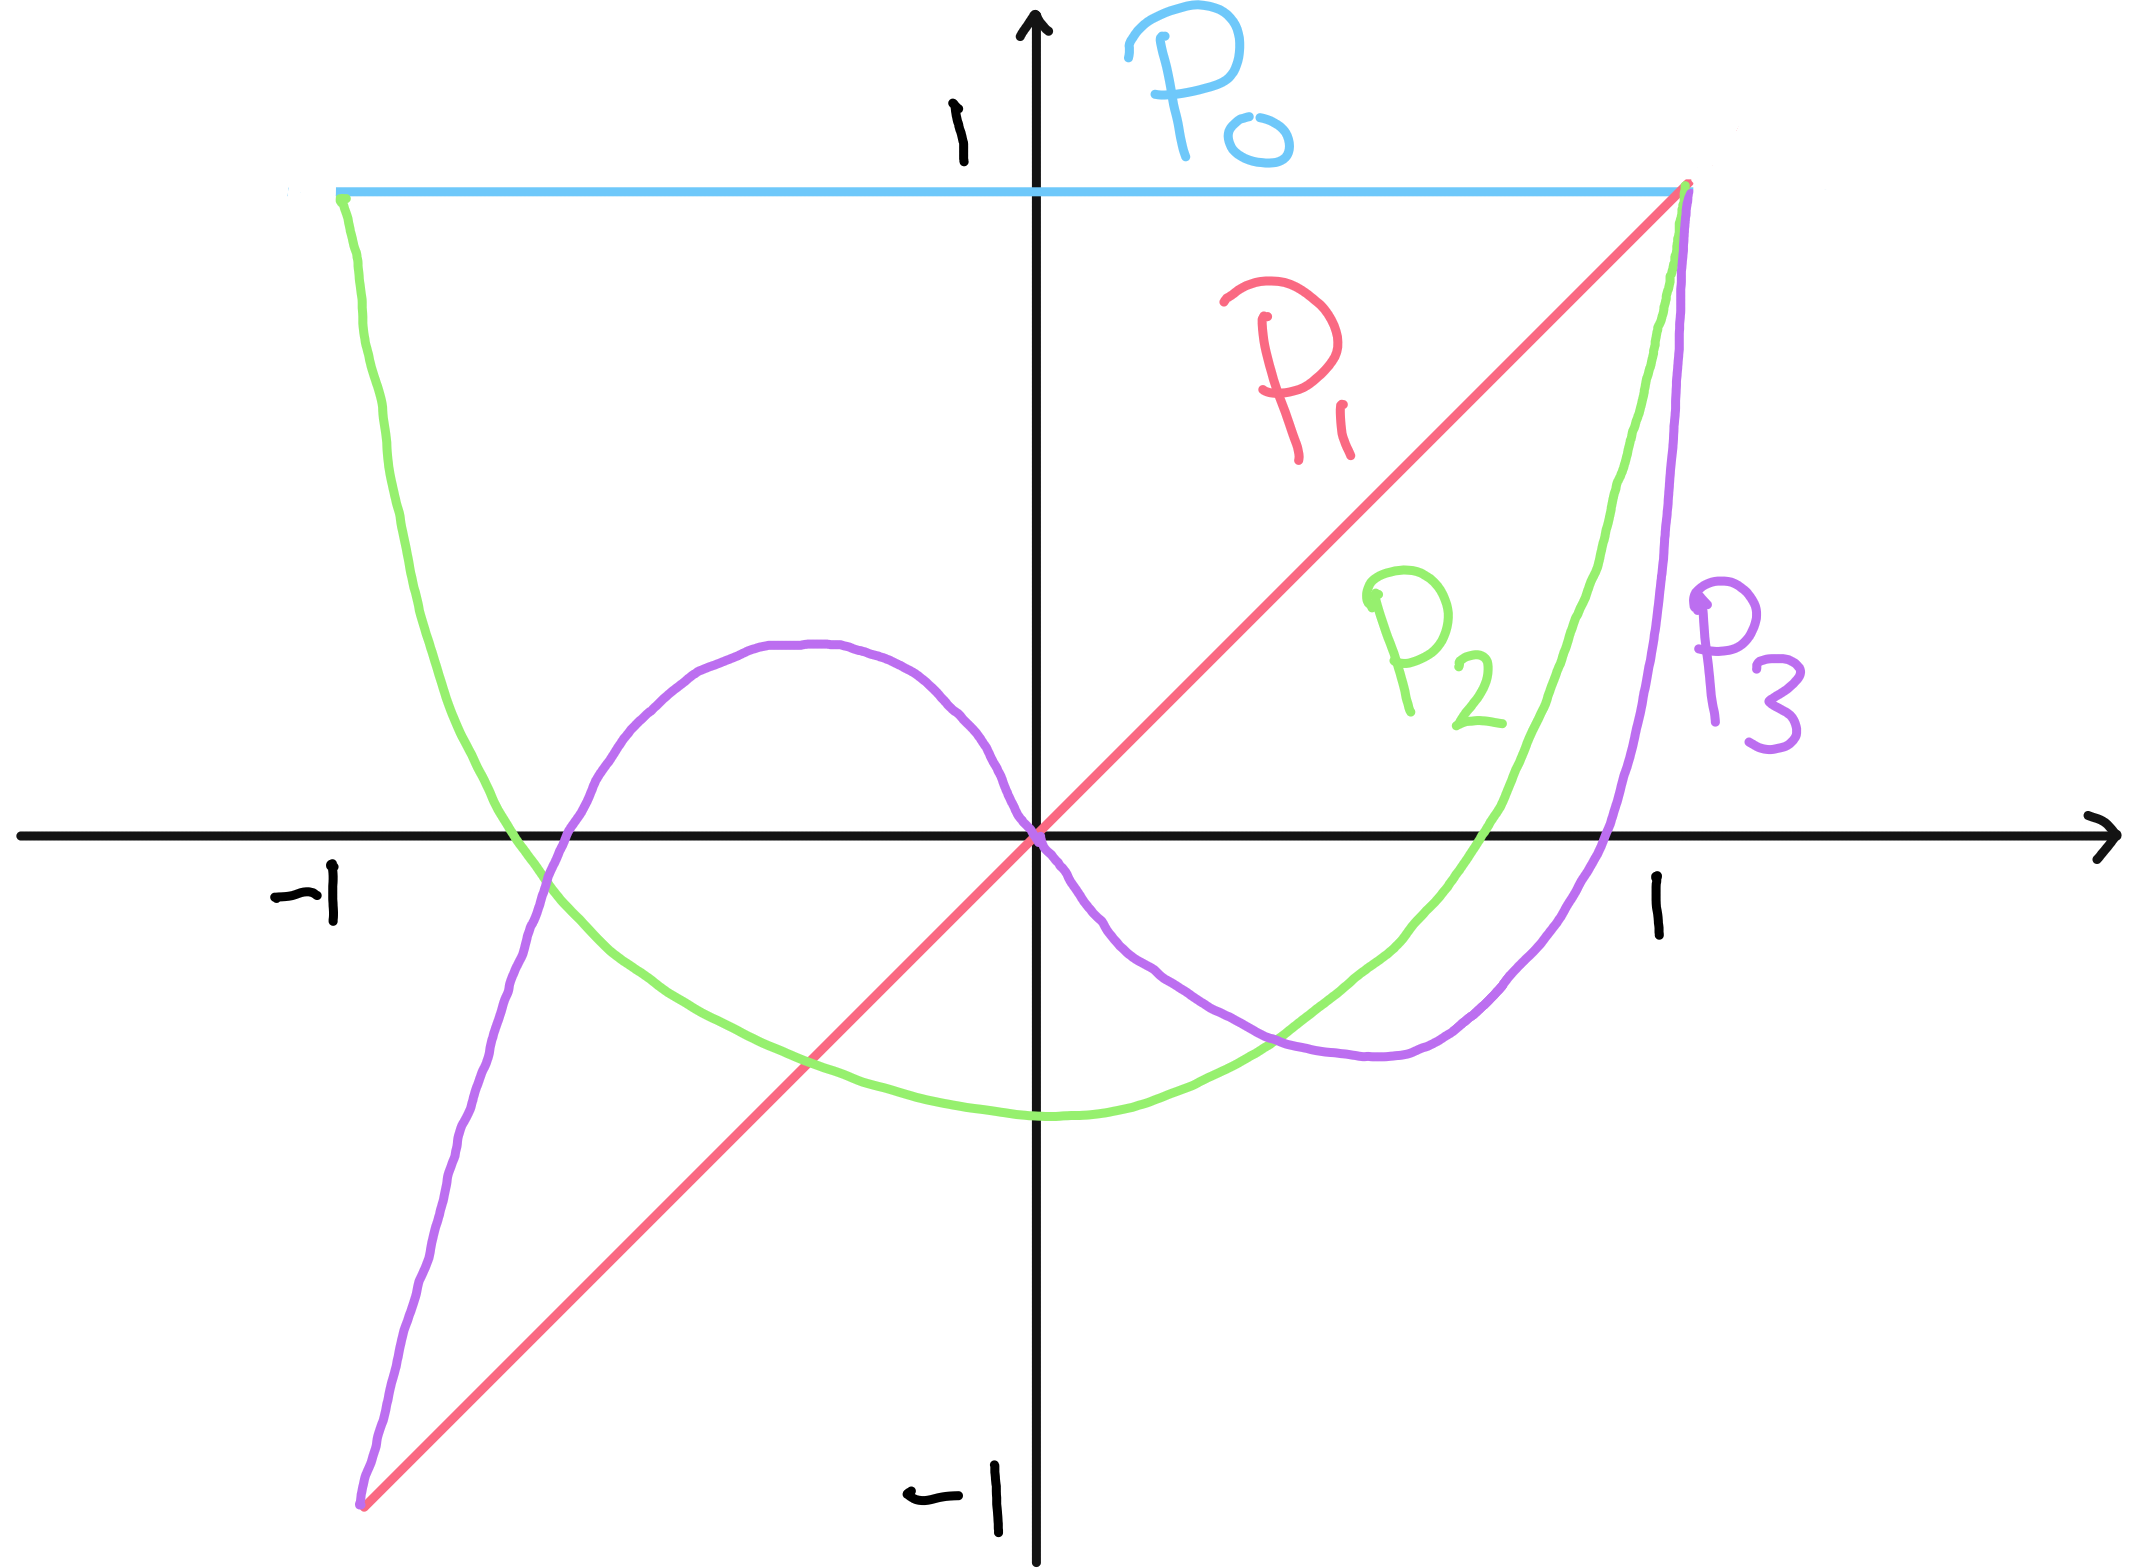
\includegraphics[height=5cm]{02-legendre} 
\end{figure}
\begin{note}
    $P_\ell(x)$ has $\ell$ zeroes.
    $P_\ell$ is odd if $\ell$ is odd, $P_\ell$ is even for even $\ell$.
\end{note} 

\subsection{Properties of Legendre polynomials}
Since Legendre polynomials come from a self-adjoint operator, they must have certain conditions, such as orthogonality.
For $n \neq m$,
\begin{align*}
    \int_{-1}^1 P_n P_m \dd{x} = 0
\end{align*}
They are also normalisable,
\addtocounter{equation}{1}
\begin{align} \label{eq:2.24}
    \int_{-1}^1 P_n^2 \dd{x} = \frac{2}{2n+1}
\end{align}
We can prove this with Rodrigues' formula (Sheet 2, Q5):
\begin{align*}
    P_n(x) = \frac{1}{2^n n!} \qty( \dv{x} )^n (x^2 - 1)^n
\end{align*}
Alternatively we could use a generating function:
\addtocounter{equation}{-2}
\begin{subequations}
    \begin{align} \label{eq:2.23a}
        \sum_{n=0}^\infty P_n(x) t^n &= \frac{1}{\sqrt{1 - 2xt + t^2}} \\
        &= 1 + \frac{1}{2}\qty(2xt - t^2) + \frac{3}{8}\qty(2xt - t^2)^2 + \dots \notag \\
        & = 1 + xt + \frac{1}{2}\qty(3x^2 - 1)t^2 + \dots \notag \\
        &= P_0 + P_1 t + P_2 t^2 + \dots \notag
    \end{align}
\end{subequations}

\begin{exercise}
    Verify $P_3$ and find $P_4$ using binomial expansion.
\end{exercise} 
There are some useful recursion relations\footnote{Derived in Example Sheet}.
\begin{align*}
    \ell(\ell + 1) P_{\ell + 1}(x) = (2 \ell + 1) x P_\ell(x) - \ell P_{\ell - 1}(x)
\end{align*}
Also,
\begin{align*}
    (2\ell + 1)P_\ell(x) = \dv{x} \qty[ P_{\ell + 1}(x) - P_{\ell - 1}(x) ]
\end{align*}

\subsection{Legendre polynomials as eigenfunctions}
Any (well-behaved) function $f(x)$ on $[-1,1]$ can be expressed as
\addtocounter{equation}{1}
\begin{align} \label{eq:2.25}
    f(x) = \sum_{\ell = 0}^\infty a_\ell P_\ell(x)
\end{align}
where
\begin{align} \label{eq:2.26}
    a_\ell = \frac{2\ell + 1}{2} \int_{-1}^1 f(x) P_\ell(x) \dd{x}
\end{align}
with no boundary conditions (e.g.\ periodicity conditions) on $f$.

\begin{exercise}
    Verify $f(x) = \frac{15}{2} x^2 - \frac{3}{2} = P_0(x) + 5 P_2(x)$ using \cref{eq:2.26}
\end{exercise} 

\subsection{Solving inhomogeneous differential equations}
\textit{This can be thought of as the general case of Fourier series discussed previously.}

Consider the problem
\begin{align} \label{eq:2.27}
    \mathcal L y = f(x) \equiv w(x) F(x)
\end{align}
on $x \in [a,b]$ assuming homogeneous boundary conditions.
Given eigenfunctions $y_n(x)$ satisfying $\mathcal L y_n = \lambda_n w y_n$, we wish to expand this solution as (recall \cref{sec:1.6})
\begin{align*}
    y(x) = \sum_n c_n y_n(x)
\end{align*}
and
\begin{align*}
    F(x) = \sum_n a_n y_n(x)
\end{align*}
where $a_n$ are known and $c_n$ are unknown.
Using \cref{eq:2.17}:
\begin{align*}
    a_n = \frac{\int_a^b w F y_n \dd{x}}{\int_a^b w y_n^2 \dd{x}}
\end{align*}
Substituting,
\begin{align*}
    \mathcal L y = \mathcal L \sum_n c_n y_n = w \sum_n c_n \lambda_n y_n = w \sum_n a_n y_n
\end{align*}
By orthogonality,
\begin{align*}
    c_n \lambda_n = a_n \implies c_n = \frac{a_n}{\lambda_n}
\end{align*}
In particular,
\begin{align} \label{eq:2.28}
    y(x) = \sum_{n=1}^\infty \frac{a_n}{\lambda_n}y_n(x)
\end{align} (assuming $\lambda_n \neq 0, \forall \; n$).

We can further generalise; we can permit a driving force, which often induces a linear response term $\widetilde\lambda w y$.
\begin{align} \label{eq:2.29}
    \mathcal L y - \widetilde \lambda w y = f(x)
\end{align}
where $\widetilde \lambda$ is fixed.
The solution \cref{eq:2.28} becomes
\begin{align} \label{eq:2.30}
    y(x) = \sum_{n=1}^\infty \frac{a_n}{\lambda_n - \widetilde \lambda} y_n(x)
\end{align} (again $\widetilde \lambda \neq \lambda_n, \forall \; n$).

\subsection{Integral solutions and Green's function}
Recall \cref{eq:2.28}
\begin{align*}
    y(x) = \sum_{n=1}^\infty \frac{a_n}{\lambda_n} y_n(x) = \sum_n \frac{y_n(x)}{\lambda_n N_n} \int_a^b w(\xi) F(\xi) y_n(\xi) \dd{\xi} \text{ by \cref{eq:2.17}}
\end{align*}
where
\begin{align*}
    N_n = \int w y_n^2 \dd{x}
\end{align*}
This then gives
\begin{align}
    y(x) &= \int_a^b \underbrace{\sum_{n=1}^\infty \frac{y_n(x) y_n(\xi)}{\lambda_n N_n}}_{G(x,\xi)} \underbrace{w(\xi) F(\xi)}_{f(\xi)} \dd{\xi} \notag\\
    &= \int_a^b G(x;\xi) f(\xi) \dd{\xi} \label{eq:2.31}
\end{align}
where
\begin{align*}
    G(x,\xi) = \sum_{n=1}^\infty \frac{y_n(x) y_n(\xi)}{\lambda_n N_n}
\end{align*}
is the eigenfunction expansion of the Green's function.
Note that the Green's function does not depend on $f$, but only on $\mathcal L$ and the boundary conditions.
In this sense, it acts like an inverse operator
\begin{align*}
    \mathcal L\inv \equiv \int \dd{\xi} G(x,\xi)
\end{align*}
analogously to how $Ax = b \implies x = A^{-1} b$ for matrix equations.
    % \part{PDEs on Bounded Domains}
    \part{PDEs on Bounded Domains}

\section{The Wave Equation}

\subsection{Waves on an elastic string}
Consider a small displacement $y(x,t)$ on a stretched string with fixed ends at $x = 0$ and $x = L$, that is, with boundary conditions
\begin{align} \label{eq:3.1}
	y(0,t) = y(L,t) = 0.
\end{align} 
and initial conditions
\begin{align} \label{eq:3.2}
	y(x, 0) = p(x),\ \frac{\partial y}{\partial t}(x,0) = q(x)
\end{align} 
We derive the equation of motion governing the motion of the string by balancing forces on a string segment $(x,x+\delta x)$ and take the limit as $\delta x \to 0$.
\begin{figure}[h] 
	\centering 
	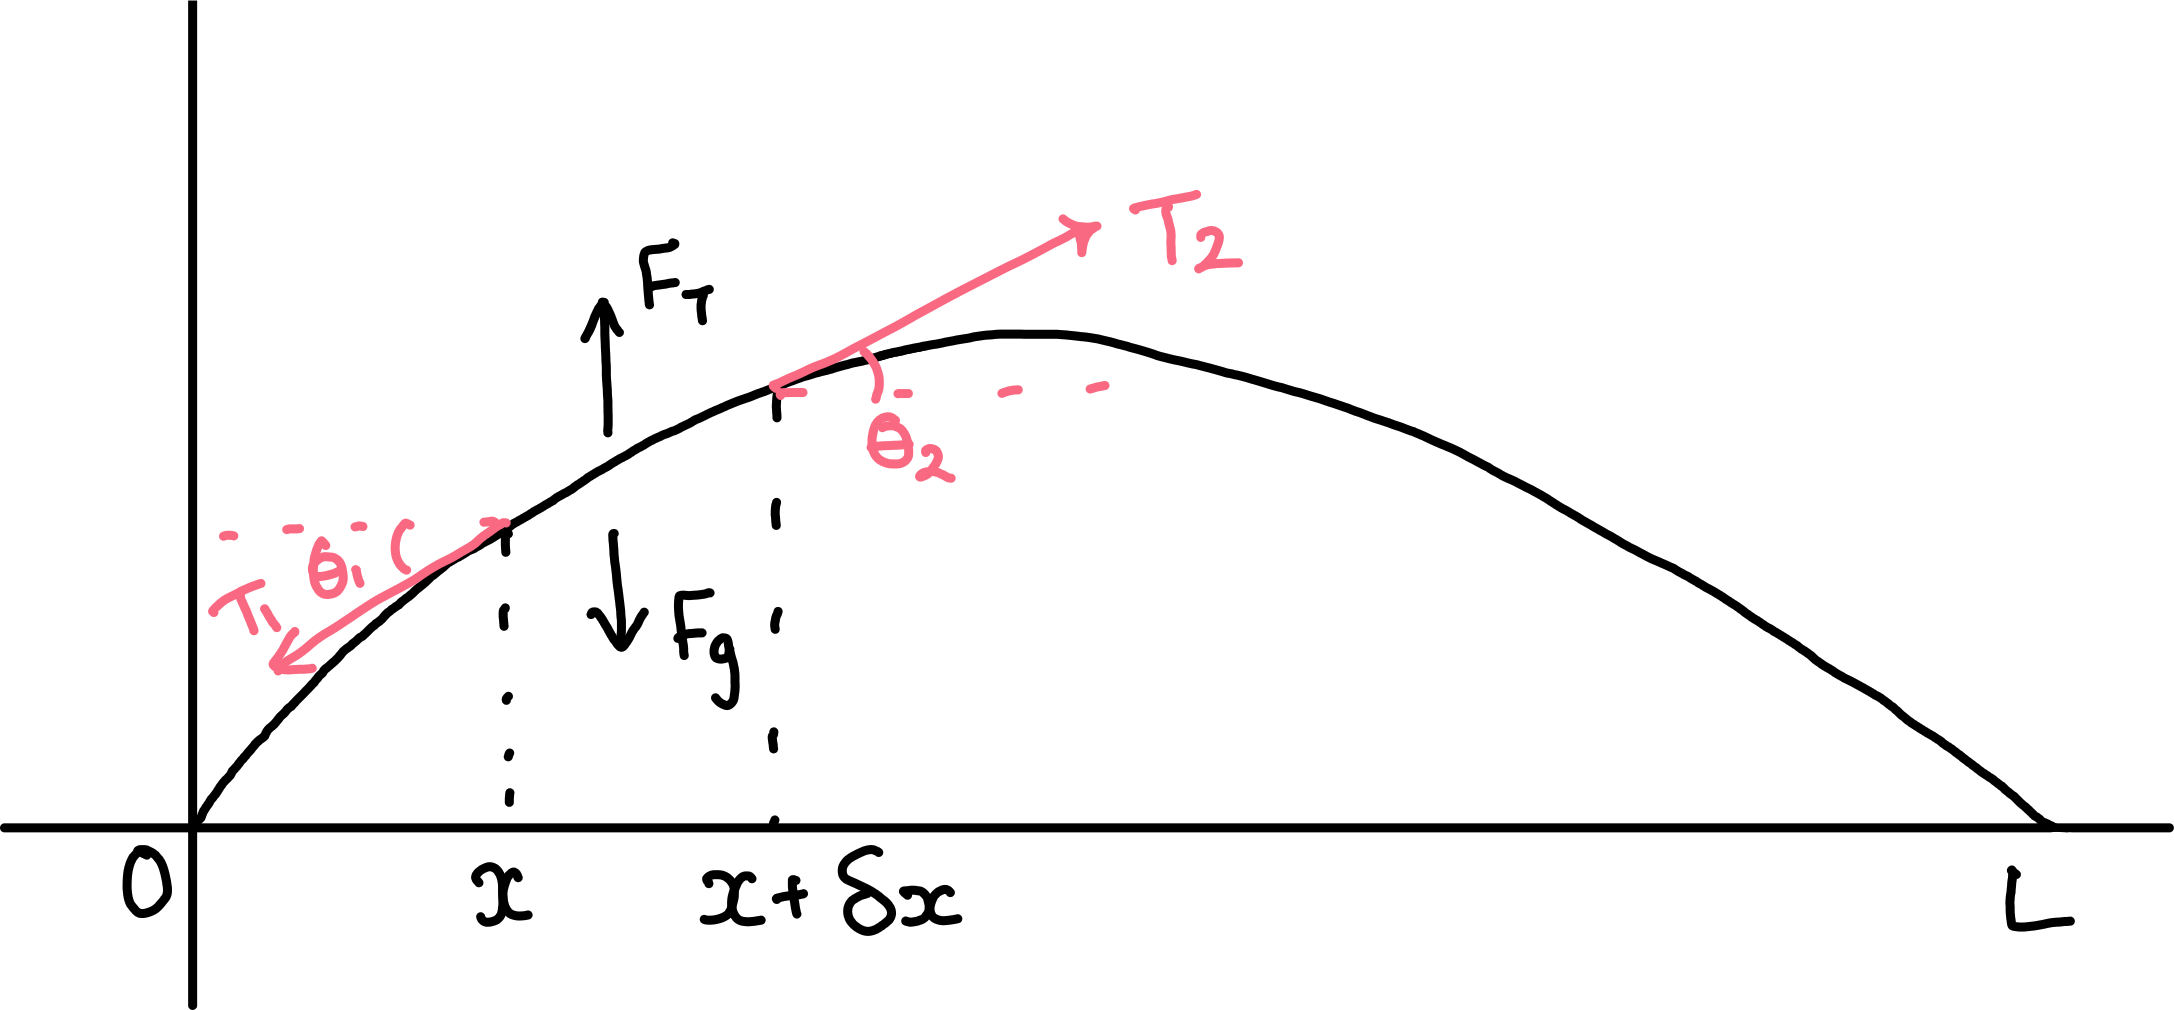
\includegraphics[height=5cm]{03-string} 
\end{figure}

Let $T_1$ be the tension force acting to the left at angle $\theta_1$ from the horizontal.
Analogously, let $T_2$ be the rightwards tension force at angle $\theta_2$.
We assume at any point on the string that $\abs{\pdv{y}{x}} \ll 1$, so the angles of the forces, $\theta_1, \theta_2$ are small.
In the $x$ dimension,
\begin{align*}
	T_1 \cos \theta_1 = T_2 \cos \theta_2 \implies T_1 \approx T_2 = T \text{ by small angle approximation}
\end{align*}
So the tension $T$ is a constant independent of $x$ up to an error of order $O\qty(\abs{\pdv{y}{x}
}^2)$.
In the $y$ dimension, since the $\theta$ are small,
\begin{align*}
	F_T = T_2 \sin \theta_2 - T_1 \sin \theta_1 \approx T \qty(\eval{\pdv{y}{x}}_{x + \delta x} - \eval{\pdv{y}{x}}_x) \approx T \pdv[2]{y}{x} \delta x
\end{align*}
By $F = ma$,
\begin{align*}
	F_T + F_g = (\mu \, \delta x) \pdv[2]{y}{t} = T \pdv[2]{y}{x} \delta x - g \mu \delta x
\end{align*}
where $F_g$ is the gravitational force and $\mu$ is the mass per unit length (linear mass density).
We define the wave speed as
\begin{align*}
	c = \sqrt{\frac{T}{\mu}} \text{ (a constant)}
\end{align*}
and find
\begin{align}
	\pdv[2]{y}{t} = \frac{T}{\mu} \pdv[2]{y}{x} - g = c^2 \pdv[2]{y}{x} - g \label{eq:3.3}
\end{align}
We often assume gravity is negligible to produce the pure wave equation
\begin{align} \label{eq:3.4}
	\frac{1}{c^2} \pdv[2]{y}{t} = \pdv[2]{y}{x}.
\end{align}
The 1D wave equation is then $\ddot{y} = c^2 y''$.

\subsection{Separation of variables}
We wish to solve the wave equation \cref{eq:3.4} subject to  boundary conditions \cref{eq:3.1} and initial conditions \cref{eq:3.2}.
Consider a possible solution of \underline{seperable form} (ansatz):
\begin{align} \label{eq:3.5}
	y(x,t) = X(x) T(t)
\end{align}
Substituting into the wave equation \cref{eq:3.4},
\begin{align*}
	\frac{1}{c^2} \ddot y = y'' \implies \frac{1}{c^2} X \ddot T = X'' T.
\end{align*}
Then
\begin{align*}
	\frac{1}{c^2}\frac{\ddot T}{T} = \frac{X''}{X}
\end{align*}
However, $\frac{\ddot T}{T}$ depends only on $t$ and $\frac{X''}{X}$ depends only on $x$.
Thus, both sides must be equal to some \textit{separation constant} $-\lambda$.
\begin{align*}
	\frac{1}{c^2}\frac{\ddot T}{T} = \frac{X''}{X} = -\lambda
\end{align*}
Hence,
\begin{align}
	X'' + \lambda X &= 0 \label{eq:3.6} \\ 
	\ddot T + \lambda c^2 T &= 0. \label{eq:3.7}
\end{align}

\subsection{Boundary conditions and normal modes}
We will begin by first solving the spatial ODE \cref{eq:3.6}.
One of $\lambda > 0, \lambda < 0, \lambda = 0$ must be true.
The boundary conditions \cref{eq:3.1} restrict the possible $\lambda$.
\begin{enumerate}
	\item First, suppose $\lambda < 0$.
	      Take $\chi^2 = -\lambda$.
	      Then,
	      \begin{align*}
		      X(x) = Ae^{\chi x} + Be^{-\chi x} = \tilde A \cosh (\chi x) + \tilde B \sinh (\chi x).
	      \end{align*}
	      The boundary conditions are $x(0) = x(L) = 0$, so only the trivial solution is possible: $\tilde A = \tilde B = 0$.
	\item Now, suppose $\lambda = 0$.
	      Then
	      \begin{align*}
		      X(x) = Ax + B.
	      \end{align*}
	      Again, the boundary conditions impose $A = B = 0$ giving only the trivial solution.
	\item Finally, the last possibility is $\lambda > 0$.
	      \begin{align*}
		      X(x) = A \cos \qty(\sqrt{\lambda} x) + B \sin \qty(\sqrt{\lambda} x)
	      \end{align*}
	      The boundary conditions give
	      \begin{align*}
		      A = 0;\quad B \sin \qty(\sqrt{\lambda} L) = 0 \implies \sqrt{\lambda} L = n \pi.
	      \end{align*}
		  The following are the eigenfunctions and eigenvalues.
		\begin{align}
			X_n(x) = B_n \sin \frac{n \pi x}{L};\quad \lambda_n = \qty(\frac{n \pi}{L})^2 \ (n > 0) \label{eq:3.8}
		\end{align}
\end{enumerate}

These are also called the \vocab{normal modes} of the system because the spatial shape in $x$ does not change in time, but the amplitude may vary. \\
The fundamental mode is the lowest frequency of vibration, given by
\begin{align*}
	n = 1 \implies \lambda_1 = \frac{\pi^2}{L^2}
\end{align*}
\begin{figure}[h] 
    \centering 
    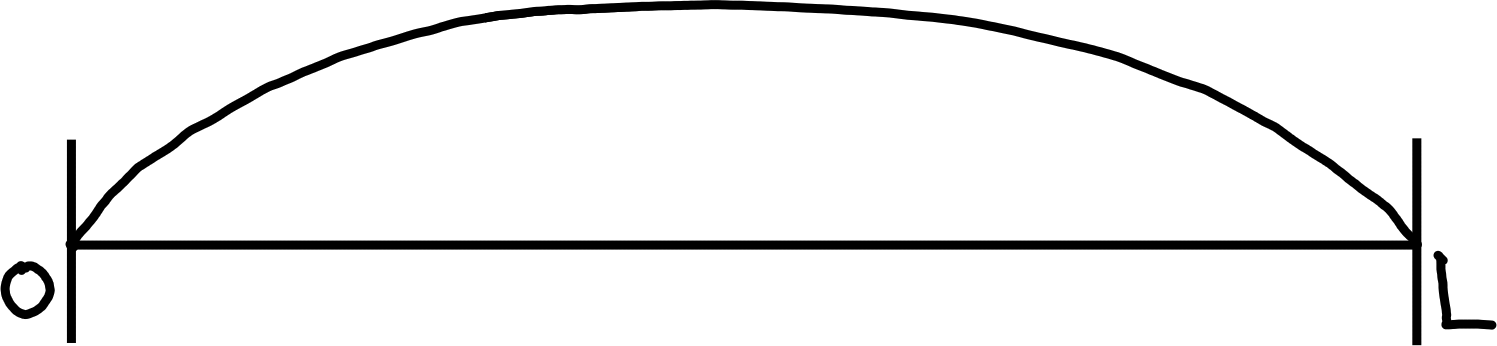
\includegraphics[height=5cm]{03-firstharmonic} 
\end{figure}
The second mode is the first overtone, and is given by
\begin{align*}
	n = 2 \implies \lambda_2 = \frac{4\pi^2}{L^2}
\end{align*}
\begin{figure}[h] 
    \centering 
    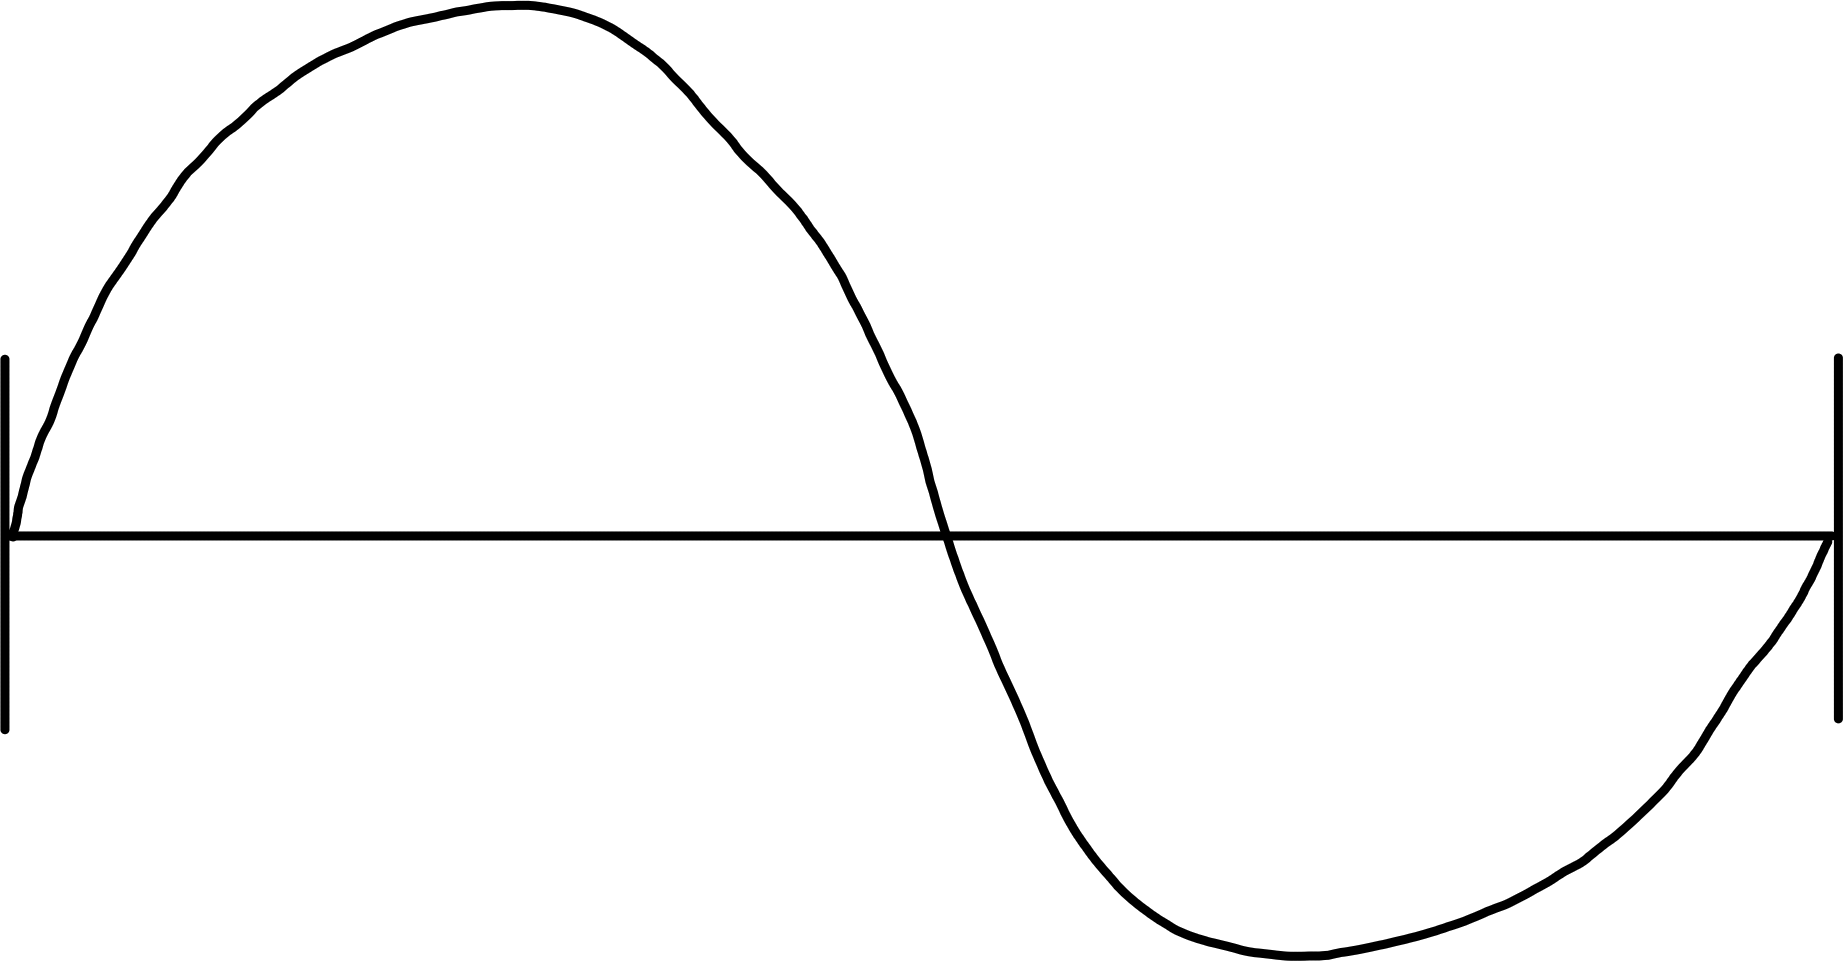
\includegraphics[height=5cm]{03-secondharmonic} 
\end{figure}

\subsection{Initial conditions and temporal solutions}
Substituting $\lambda_n$ into the time ODE \cref{eq:3.7},
\begin{align*}
	\ddot T + \frac{n^2 \pi^2 c^2}{L^2}T = 0.
\end{align*}
Hence,
\begin{align} \label{eq:3.9}
	T_n(t) = C_n \cos \frac{n \pi c t}{L} + D_n \sin \frac{n \pi c t}{L}.
\end{align}

Therefore, a specific solution of the wave equation, \cref{eq:3.4}, satisfying the boundary conditions, \cref{eq:3.1}, is (absorbing the $B_n$ into the $C_n, D_n$):
\begin{align*}
	y_n(x,t) = T_n(t) X_n(x) = \qty(C_n \cos \frac{n \pi c t}{L} + D_n \sin \frac{n \pi c t}{L}) \sin \frac{n \pi x}{L}
\end{align*}

\begin{exercise}
	Verify it's a solution.
\end{exercise} 

Since the wave equation \cref{eq:3.4} is linear (and b.c.s \cref{eq:3.1} are homogenous) we can add the solutions (the $y_n$) together to find \vocab{general string solution}
% To find a particular solution for a given set of initial conditions, we must consider a linear superposition of all possible $y_n$.
\begin{align} \label{eq:3.10}
	y(x,t) = \sum_{n=1}^\infty \qty(C_n \cos \frac{n \pi c t}{L} + D_n \sin \frac{n \pi c t}{L}) \sin \frac{n \pi x}{L}.
\end{align}
By construction, this $y(x,t)$ satisfies the boundary conditions, so now we can impose the initial conditions \cref{eq:3.2}:
\begin{align*}
	y(x,0) = p(x) = \sum_{n=1}^\infty C_n \sin \frac{n \pi x}{L}
\end{align*}
We can find the $C_n$ using standard Fourier series techniques \cref{eq:1.12}, since this is exactly a half-range sine series.
Further,
\begin{align*}
	\pdv{y(x,0)}{t} = q(x) = \sum_{n=1}^\infty \frac{n \pi c}{L} D_n \sin \frac{n \pi x}{L}
\end{align*}
Again we can solve for the $D_n$ in a similar way.
Using \cref{eq:1.12}:
\begin{align}
	\begin{aligned} \label{eq:3.11}
		C_n &= \frac{2}{L} \int_0^L p(x) \sin \frac{n \pi x}{L} \dd{x} \\
		D_n &= \frac{2}{n \pi c} \int_0^L q(x) \sin \frac{n \pi x}{L} \dd{x}
	\end{aligned}
\end{align} 

Hence \cref{eq:3.11} is the solution to \cref{eq:3.4} satisfying \cref{eq:3.1,eq:3.2}.

\begin{example}
	Consider the initial condition of a see-saw wave parametrised by $\xi$, and let $L = 1$.
	This can be visualised as plucking the string at position $\xi$.
	\begin{align*}
		y(x,0) = p(x) = \begin{cases}
			x(1-\xi) & 0 \leq x < \xi \\
			\xi(1-x) & \xi \leq x < 1
		\end{cases}
	\end{align*}
	We also define
	\begin{align*}
		\pdv{y(x,0)}{t} = q(x) = 0
	\end{align*}
	The Fourier series \cref{eq:1.8} for $p$ is given by
	\begin{align*}
		C_n = \frac{2 \sin n \pi \xi}{(n \pi)^2};\quad D_n = 0
	\end{align*}
	Hence the solution to the wave equation is
	\begin{align*}
		y(x,t) = \sum_{n=1}^\infty \frac{2}{(n \pi)^2} \sin n \pi \xi \sin n \pi x \cos n \pi c t
	\end{align*}
	Take $\xi = \frac{1}{2}, C_{2m} = 0, C_{2m - 1} = \frac{2 (-1)^{m + 1}}{((2m-1) \pi)^2}$ (odd only), e.g. Guitar has $\frac{1}{4} \leq \xi \leq \frac{1}{3}$, Violin $\xi \approx \frac{1}{7}$.
\end{example}

\begin{aside}{Solution in characterstic coordinates}
	Recall sine/cosine summation identities (before \cref{eq:1.1}) which means our general solution \cref{eq:3.10} becomes
	\begin{align}
		y(x, t) &= \frac{1}{2} \sum_{n=1}^{\infty} \qty[C_n \sin \frac{n \pi}{L} (x-ct) + D_n \cos \frac{n \pi}{L} (x - ct) + C_n \sin \frac{n \pi}{L} (x + ct) + D_n \cos \frac{n \pi}{L} (x + ct)] \notag \\
		&\equiv f(x - ct) + g(x + ct) \label{eq:3.12}
	\end{align} 
	The standing wave solution \cref{eq:3.10} is made up of a right-moving wave (along characteristic $x - ct = \eta$, $\eta$ a constant) and a left-moving wave ($x + ct = \xi$, $\xi$ a constant) i.e. a general solution with arbitrary $f, g$ (see later).

	\underline{Special case}: $q(x) = 0$ in \cref{eq:3.1} $\implies f = g = \frac{1}{2} D$ at $t = 0$.
	\begin{figure}[h] 
		\centering 
		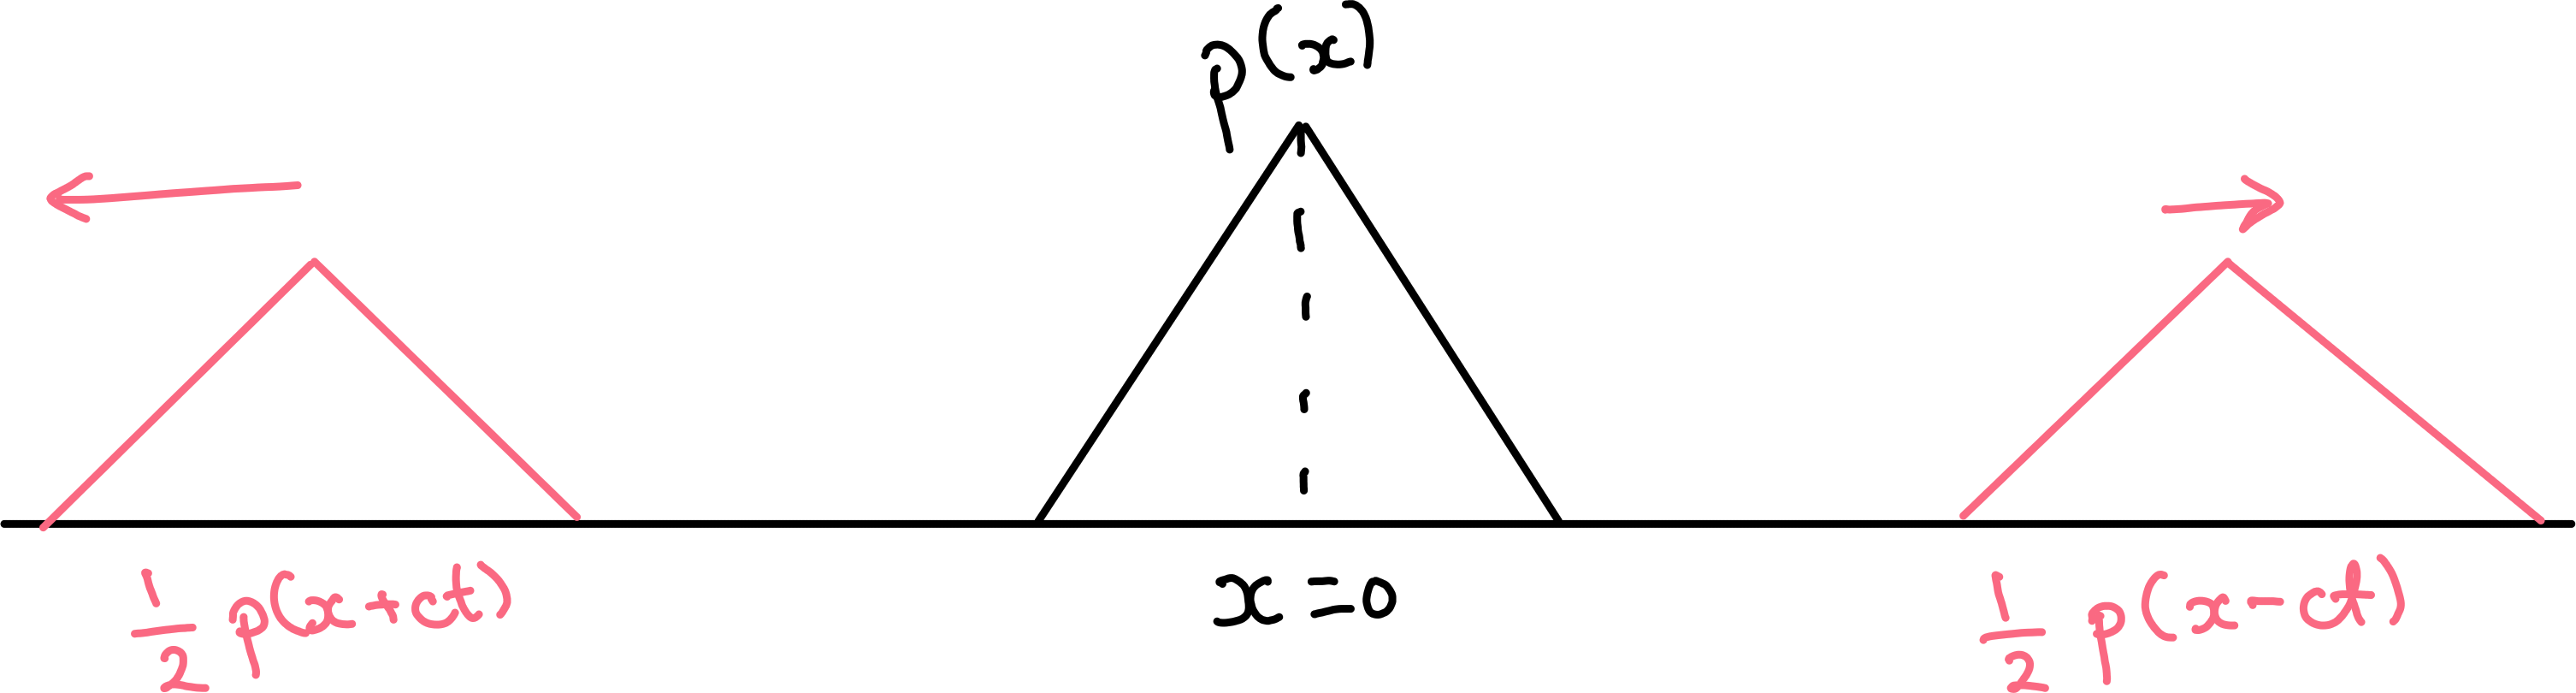
\includegraphics[height=5cm]{03-specialcase} 
	\end{figure}
	
\end{aside} 

\subsection{Separation of variables methodology}
A general strategy for solving higher-dimensional partial differential equations is as follows.
\begin{enumerate}
	\item Obtain a linear PDE system, using boundary and initial conditions.
	\item Separate variables to yield decoupled ODEs.
	\item Impose homogeneous boundary conditions to find eigenvalues and eigenfunctions.
	\item Use these eigenvalues (constants of separation) to find the eigenfunctions in the other variables.
	\item Sum over the products of separable solutions to find the general series solution.
	\item Determine coefficients for this series using the initial conditions.
\end{enumerate}
% \begin{example}
% 	We will solve the wave equation instead in characteristic coordinates.
% 	Recall the sine and cosine summation identities:
% 	\begin{align*}
% 		y(x,t) & = \frac{1}{2} \sum_{n=1}^\infty \Bigg[ \qty(C_n \sin \frac{n \pi}{L}(x-ct) + D_n \cos \frac{n \pi}{L}(x-ct)) \\&
% 		+ \qty(C_n \sin \frac{n \pi}{L}(x+ct) - D_n \cos \frac{n \pi}{L}(x+ct)) \Bigg]                                        \\
% 		       & = f(x-ct) + g(x+ct)
% 	\end{align*}
% 	The standing wave solution can be interpreted as a superposition of a right-moving wave and a left-moving wave.
% 	A special case is $q(x) = 0$, implying $f = g = \frac{1}{2} p$.
% 	Then,
% 	\begin{align*}
% 		y(x,t) = \frac{1}{2}\qty[p(x-ct) + p(x+ct)]
% 	\end{align*}
% \end{example}

\subsection{Energy of oscillations}
A vibrating string has kinetic energy due to its motion.
\begin{align*}
	\text{Kinetic energy} = \frac{1}{2} \mu \int_0^L \qty(\pdv{y}{t})^2 \dd{x}
\end{align*}
It has potential energy  due to stretching by $\Delta x$ given by
\begin{align*}
	\text{Potential energy} = T \Delta x = T \int_c^T \qty(\underbrace{\sqrt{1 + \qty(\pdv{y}{x})^2}}_\text{arc length $s$} -1)\dd{x} \approx \frac{1}{2} T \int_0^L \qty(\pdv{y}{x})^2 \dd{x}
\end{align*}
assuming that the disturbances on the string are small, that is, $\abs{\pdv{y}{x}} \ll 1$.
The total energy on the string, given $c^2 = T/\mu$, is given by
\begin{align} \label{eq:3.13}
	E = \frac{1}{2}\mu \int_0^L \qty[\qty(\pdv{y}{t})^2 + c^2 \qty(\pdv{y}{x})^2] \dd{x}
\end{align}
Substituting the solution \cref{eq:3.10}, using the orthogonality conditions \cref{eq:1.1},
\begin{align}
	E &= \frac{1}{2}\mu \sum_{n=1}^\infty \int_0^L \Bigg[\qty(-\frac{n \pi c}{L} C_n \sin \frac{n \pi c t}{L} + \frac{n \pi c}{L} D_n \cos \frac{n \pi c t}{L})^2 \sin^2 \frac{n \pi x}{L}\notag \\
	&+ c^2 \qty(C_n \cos \frac{n \pi c t}{L} + D_n \sin \frac{n \pi c t}{L})^2 \frac{n^2 \pi^2}{L^2} \cos^2 \frac{n \pi x}{L} \Bigg] \dd{x} \notag \\
	&= \frac{1}{4} \mu \sum_{n=1}^\infty \frac{n^2 \pi^2 c^2}{L} \qty(C_n^2 + D_n^2) \label{eq:3.14}
\end{align}
which is an analogous result to Parseval's theorem.
This is true since \begin{align*}
	\int \cos^2 \frac{n \pi x}{L}\dd{x} = \frac{1}{2}
\end{align*} and $\cos^2 + \sin^2 = 1$.
We can think of this energy as the sum over all the normal modes of the energy in that specific mode.
Note that this quantity is constant over time (no dissipation).

\subsection{Wave reflection and transmission}
Recall the travelling wave solution \cref{eq:3.12}.
The travelling wave has left-moving and right-moving modes.
A \vocab{simple harmonic} travelling wave is
\begin{align*}
	y = \Re\qty[ A e^{i \omega(t-x/c)} ] = A \cos \qty[\omega(t-x/c) + \phi]
\end{align*}
where the phase $\phi$ is equal to $\arg A$, and the wavelength $\lambda$ is $2 \pi c / \omega$.
In further discussion, we assume only the real part is used.

Consider a density discontinuity on the string at $x = 0$ with the following properties.
\begin{align*}
	\mu = \begin{cases}
		\mu_- & \text{for } x < 0 \\
		\mu_+ & \text{for } x > 0
	\end{cases} \implies c = \begin{cases}
		c_- = \sqrt{\frac{T}{\mu_-}} & \text{for } x < 0 \\
		c_+ = \sqrt{\frac{T}{\mu_+}} & \text{for } x > 0 \\
	\end{cases}
\end{align*}
assuming a constant tension $T$.
As a wave from the negative direction approaches the discontinuity, some of the wave will be reflected, given by $B e^{i \omega(t + x/c_-)}$, and some of the wave will be transmitted, given by $D e^{i \omega(t - x/c_+)}$.
\begin{figure}[h] 
    \centering 
    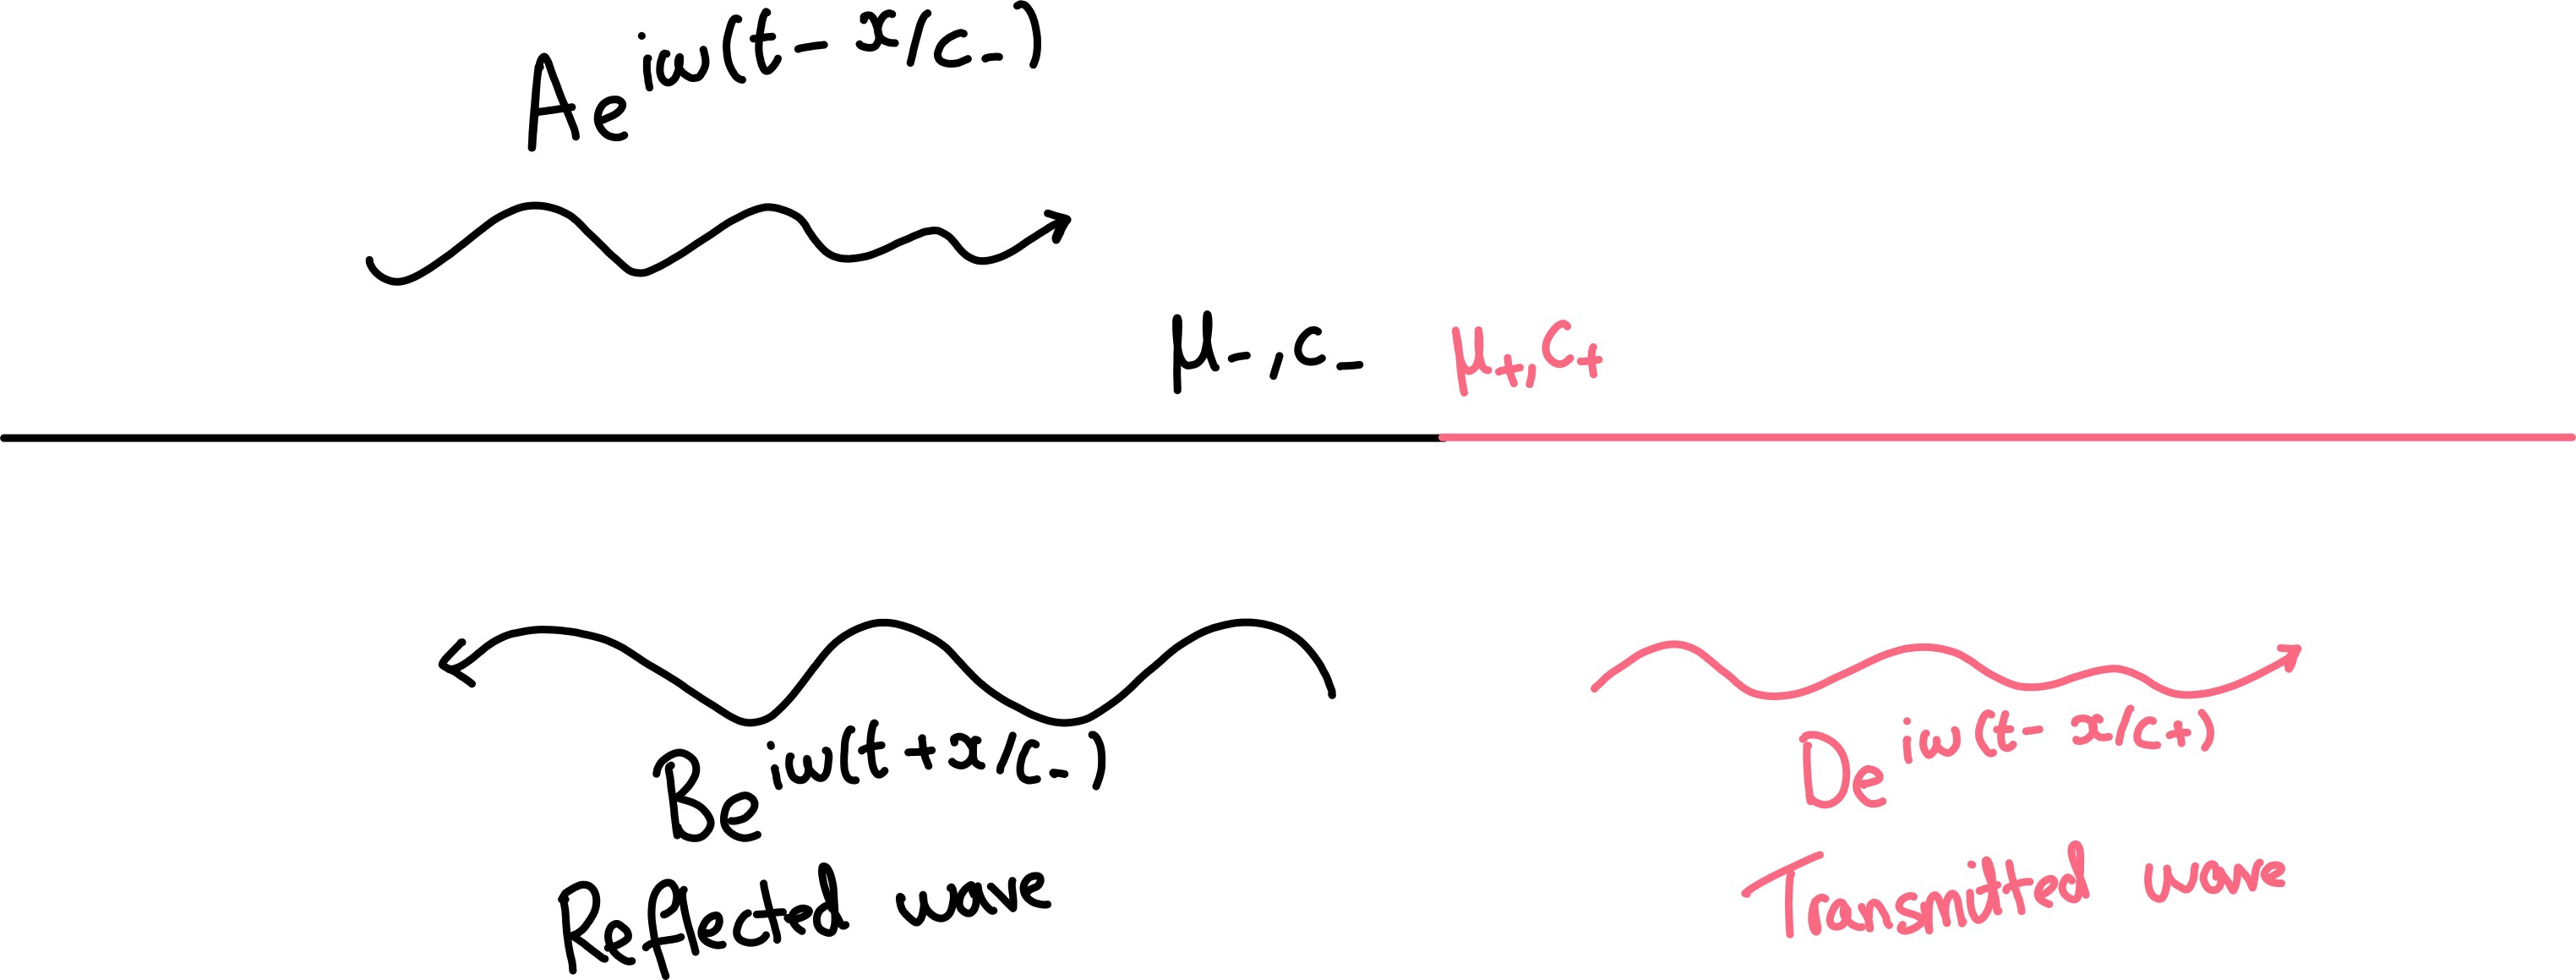
\includegraphics[height=5cm]{03-densitydiscon} 
\end{figure}
The boundary conditions at $x = 0$ are
\begin{enumerate}
	\item $y$ is continuous for all $t$ (the string does not break), so
	\begin{equation}
		A + B = D \tag{$\ast$}
	\end{equation}
	\item The forces balance, $T \eval{\pdv{y}{x}}_{x = 0^-} = T \eval{\pdv{y}{x}}_{x = 0^+}$ which means $\pdv{y}{x}$ must be continuous for all $t$.
	This gives
	\begin{equation}
		\frac{-i\omega A}{c_-} + \frac{i \omega B}{c_-} = \frac{-i \omega D}{c_+} \tag{$\dagger$}
	\end{equation}
\end{enumerate}
We can eliminate $B$ from $(\ast)$ by subtracting $\frac{c_-}{i \omega}(\dagger)$.
\begin{align*}
	2A = D + D \frac{c_-}{c_+} = \frac{D}{c_+}(c_+ + c_-)
\end{align*}
Hence, given $A$, we have the solution for the transmitted amplitude and reflected amplitude to be
\setcounter{equation}{15}
\begin{align} \label{eq:3.16}
	D = \frac{2 c_+}{c_- + c_+} A;\quad B = \frac{c_+ - c_-}{c_- + c_+}
\end{align}
In general $A, B, D$ are complex, hence different phase shifts are possible.

There are a number of limiting cases, for example
\begin{enumerate}
	\item If $c_- = c_+$ we have $D = A$ and $B = 0$ so we have full transmission and no reflection.
	\item (Dirichlet boundary conditions) If $\frac{\mu_+}{\mu_-} \to \infty$, this models a fixed end at $x = 0$.
	      We have $\frac{c_+}{c_-} \to 0$ giving $D = 0$ and $B = -A$.
	      Notice that the reflection has occurred with opposite phase, $\phi = \pi$.
	\item (Neumann boundary conditions) Consider $\frac{\mu_+}{\mu_-} \to 0$, this models a free end.
	      Then $\frac{c_+}{c_-} \to \infty$ giving $D = 2A$, $B = A$.
	      This gives total reflection but with the same phase.
\end{enumerate}

\subsection{Wave equation in 2D plane polar coordinates}
Consider the two-dimensional wave equation for $u(r,\theta,t)$ given by
\begin{align} \label{eq:3.17}
	\frac{1}{c^2} \pdv[2]{u}{t} = \laplacian u
\end{align}
with boundary conditions at $r = 1$ on a unit disc given by
\begin{align} \label{eq:3.18}
	u(1,\theta,t) = 0 \quad \text{(fixed rim)}
\end{align}
and initial conditions for $t = 0$ given by
\begin{align} \label{eq:3.19}
	u(r,\theta,0) = \phi(r,\theta);\quad \pdv{u}{t}(r,\theta,0) = \psi(r,\theta)
\end{align}

\subsubsection{Temporal Seperation}
Suppose that this equation is separable.
First, let us consider temporal separation.
Suppose that
\begin{align} \label{eq:3.20}
	u(r,\theta,t) = T(t) V(r,\theta)
\end{align}
Then substitute into \cref{eq:3.17}
\begin{align}
	\ddot T + \lambda c^2 T &= 0 \label{eq:3.21} \\
	\laplacian V + \lambda V &= 0 \label{eq:3.22}
\end{align}
In plane polar coordinates, we can write the spatial equation \cref{eq:3.22} as
\begin{align*}
	\pdv[2]{V}{r} + \frac{1}{r} \pdv{V}{r} + \frac{1}{r^2}\pdv[2]{V}{\theta} + \lambda V = 0
\end{align*}
\subsubsection{Spatial Seperation}
We will perform another separation, supposing
\begin{align*}
	V(r,\theta) = R(r) \Theta(\theta).
\end{align*}
Substitute into \cref{eq:3.22}
\begin{align}
	\Theta'' + \mu \Theta &= 0 \label{eq:3.23} \\
	r^2 R'' + r R' + \qty(\lambda r^2 - \mu) R &= 0 \label{eq:3.24}
\end{align}
where $\lambda, \mu$ are the separation constants.
\subsubsection{Polar Solution}
The polar solution is constrained by periodicity $\Theta(0) = \Theta(2 \pi)$, since we are working on a disc.
We also consider only $\mu > 0$.
The eigenvalue is then given by $\mu = m^2$, where $m \in \mathbb N \cup \{0\}$.
\begin{align} \label{eq:3.25}
	\Theta_m(\theta) = A_m \cos m \theta + B_m \sin m \theta
\end{align}
Or, in complex exponential form,
\begin{align*}
	\Theta_m(\theta) = C_m e^{im\theta};\quad m \in \mathbb Z
\end{align*}

\subsection{Radial Equations}
We can solve the radial equation \cref{eq:3.24} (in the previous subsection) by converting it first into Sturm-Liouville form \cref{eq:2.7}, which can be accomplished by dividing by $r$ with $\mu = m^2$.
\begin{align} \label{eq:3.26}
	\dv{r} \qty(r R') - \frac{m^2}{r} = -\lambda r R \quad (0 \leq r \leq 1)
\end{align}
where $p(r) = r, q(r) = \frac{m^2}{r}, w(r) = r$, with self-adjoint boundary conditions with $R(1) = 0$.
We will require $R$ is bounded at $R(0)$, and since $p(0) = 0$ there is a regular singular point at $r = 0$.

\subsubsection{Bessel's equation}
This particular equation for $R$ is known as Bessel's equation.
We will first substitute $z \equiv \sqrt{\lambda} r$ in \cref{eq:3.26}, then we find the usual form of Bessel's equation\footnote{May also be written as $(z R')' + (z - m^2 / z) R = 0$},
\begin{align} \label{eq:3.27}
	z^2 \dv[2]{R}{z} + z \dv{R}{z} + (z^2 - m^2)R = 0
\end{align}

\subsubsection{Frobenius Solution}
We can use the method of Frobenius by substituting the following power series:
\begin{align*}
	R = z^p \sum_{n=0}^\infty a_n z^n
\end{align*}
to find
\begin{align*}
	\sum_{n=0}^\infty \qty[ a_n (n+p)(n+p-1) z^{n+p} + (n+p) z^{n+p} + z^{n+p+2} + m^2 z^{n+p} ] = 0
\end{align*}
Equating powers of $z$, we can find the indicial equation
\begin{align*}
	p^2 - m^2 = 0 \implies p = m, -m
\end{align*}
The regular solution, given by $p = m$, has recursion relation
\begin{align*}
	(n+m)^2 a_n + a_{n-2} - m^2 a_n = 0
\end{align*}
which gives
\begin{align*}
	a_n = \frac{-1}{n(n+2m)} a_{n-2}
\end{align*}
Hence, we can find
\begin{align*}
	a_{2n} = a_0 \frac{(-1)^n}{2^{2n} n!
		(n+m)(n+m-1) \dots (m+1)}
\end{align*}
If, by convention, we let
\begin{align*}
	a_0 = \frac{1}{2^m m!}
\end{align*}
we can then write the \textit{Bessel function of the first kind} by
\begin{align} \label{eq:3.28}
	J_m(z) = \qty(\frac{z}{2})^m \sum_{n=0}^\infty \frac{(-1)^n}{n!
		(n+m)!} \qty(\frac{z}{2})^{2n}
\end{align}

\begin{exercise}
	Use $y = \sqrt{z} R$ in Bessel's eqn \cref{eq:3.27} to find $y'' + y (1 + \frac{1}{4z} - \frac{m^2}{z^2})$.
	So, as $z \to \infty$, $y'' = -y$ so we have solns $R = \frac{1}{\sqrt{z}} (A \cos z + B \sin z)$.
\end{exercise}

Also works for $m = \mu$ ($\mu \notin \mathbb{Z}$) if $(n + m)! \to \Gamma(n + m + 1)$.
Second soln with $p = -m$ (integer) is the Neuman function (Bessel function of second kind).
\begin{align*}
	Y_m(z) = \lim_{\mu \to m} \frac{J_\mu \cos(\mu \pi) - J_{-\mu}(z)}{\sin \mu \pi}
\end{align*} 

\begin{exercise}
	Use \cref{eq:3.28} to show that $\frac{d}{dz} (z^m J_m(z)) = z^m J_{m-1}(z)$ and hence
	\begin{align} \label{eq:3.29}
		J'_m(z) + \frac{m}{z} J_m(z) = J_{m-1}(z)
	\end{align}
	Repeat with $z^{-m}$ to find \underline{recursion relations}
	\begin{align} \label{eq:3.30}
		\begin{aligned}
			J_{m-1}(z) + J_{m+1}(z) &= \frac{2m}{z} J_m(z) \\
			J_{m-1}(z) - J_{m+1}(z) &= 2 J'_m(z)
		\end{aligned}
	\end{align} 
\end{exercise} 

\subsection{Asymptotic behaviour of Bessel functions}
If $z$ is small, the leading-order behaviour of $J_m(z)$ is
\begin{align}
	J_0(z) & \approx 1 \notag \\
	J_m(z) & \approx \frac{1}{m!} \qty(\frac{z}{2})^m \notag \\
	Y_0(z) &\to \frac{2}{\pi} \ln(\frac{z}{2}) \notag \\
	Y_m(z) &\to - \frac{(m-1)!}{\pi} (\frac{2}{z})^m \label{eq:3.31}
\end{align}
Now, let us consider large $z$.
In this case, the function becomes oscillatory;
\begin{align}
	J_m(z) &\approx \sqrt{\frac{2}{\pi z}} \cos(z - \frac{m \pi}{2} - \frac{\pi}{4}) \label{eq:3.32} \\
	Y_m(z) &\approx \sqrt{\frac{2}{\pi z}} \sin(z - \frac{m \pi}{2} - \frac{\pi}{4}) \notag
\end{align}

\subsection{Zeroes of Bessel functions $J_m(z)$}
We can see from the asymptotic behaviour that there are infinitely many zeroes of the Bessel functions of the first kind as $z \to \infty$.
We define $j_{mn}$ to be the $n$th zero of $J_m$, for $z > 0$.
Approximately using \cref{eq:3.32},
\begin{align*}
	\cos(z - \frac{m \pi}{2} - \frac{\pi}{4}) = 0 \implies z - \frac{m \pi}{2} - \frac{\pi}{4} = n \pi - \frac{\pi}{2} \quad \text{(modal point)}
\end{align*}
Hence
\begin{align*}
	z \approx n \pi + \frac{m \pi}{2} - \frac{\pi}{4} \equiv \widetilde j_{mn}
\end{align*}

\begin{aside}{Non-examinable}
	Accuracy, 
	\begin{align} \label{eq:3.33}
		\qty| \frac{j_{mn} - \widetilde j_{mn}}{j_{mn}} | < \frac{0.1}{n} \text{ for } n > \frac{m^2}{2}.
	\end{align}
\end{aside} 

For $J_0(z)$ actual values are $J_{01} = 2.405$, $j_{02} = 5.520$, $j_{03} = 8.653$, $j_{0n} = n \pi - \frac{\pi}{4}$ (precision $\approx 1\%/n$).

\begin{figure}[h] 
    \centering 
    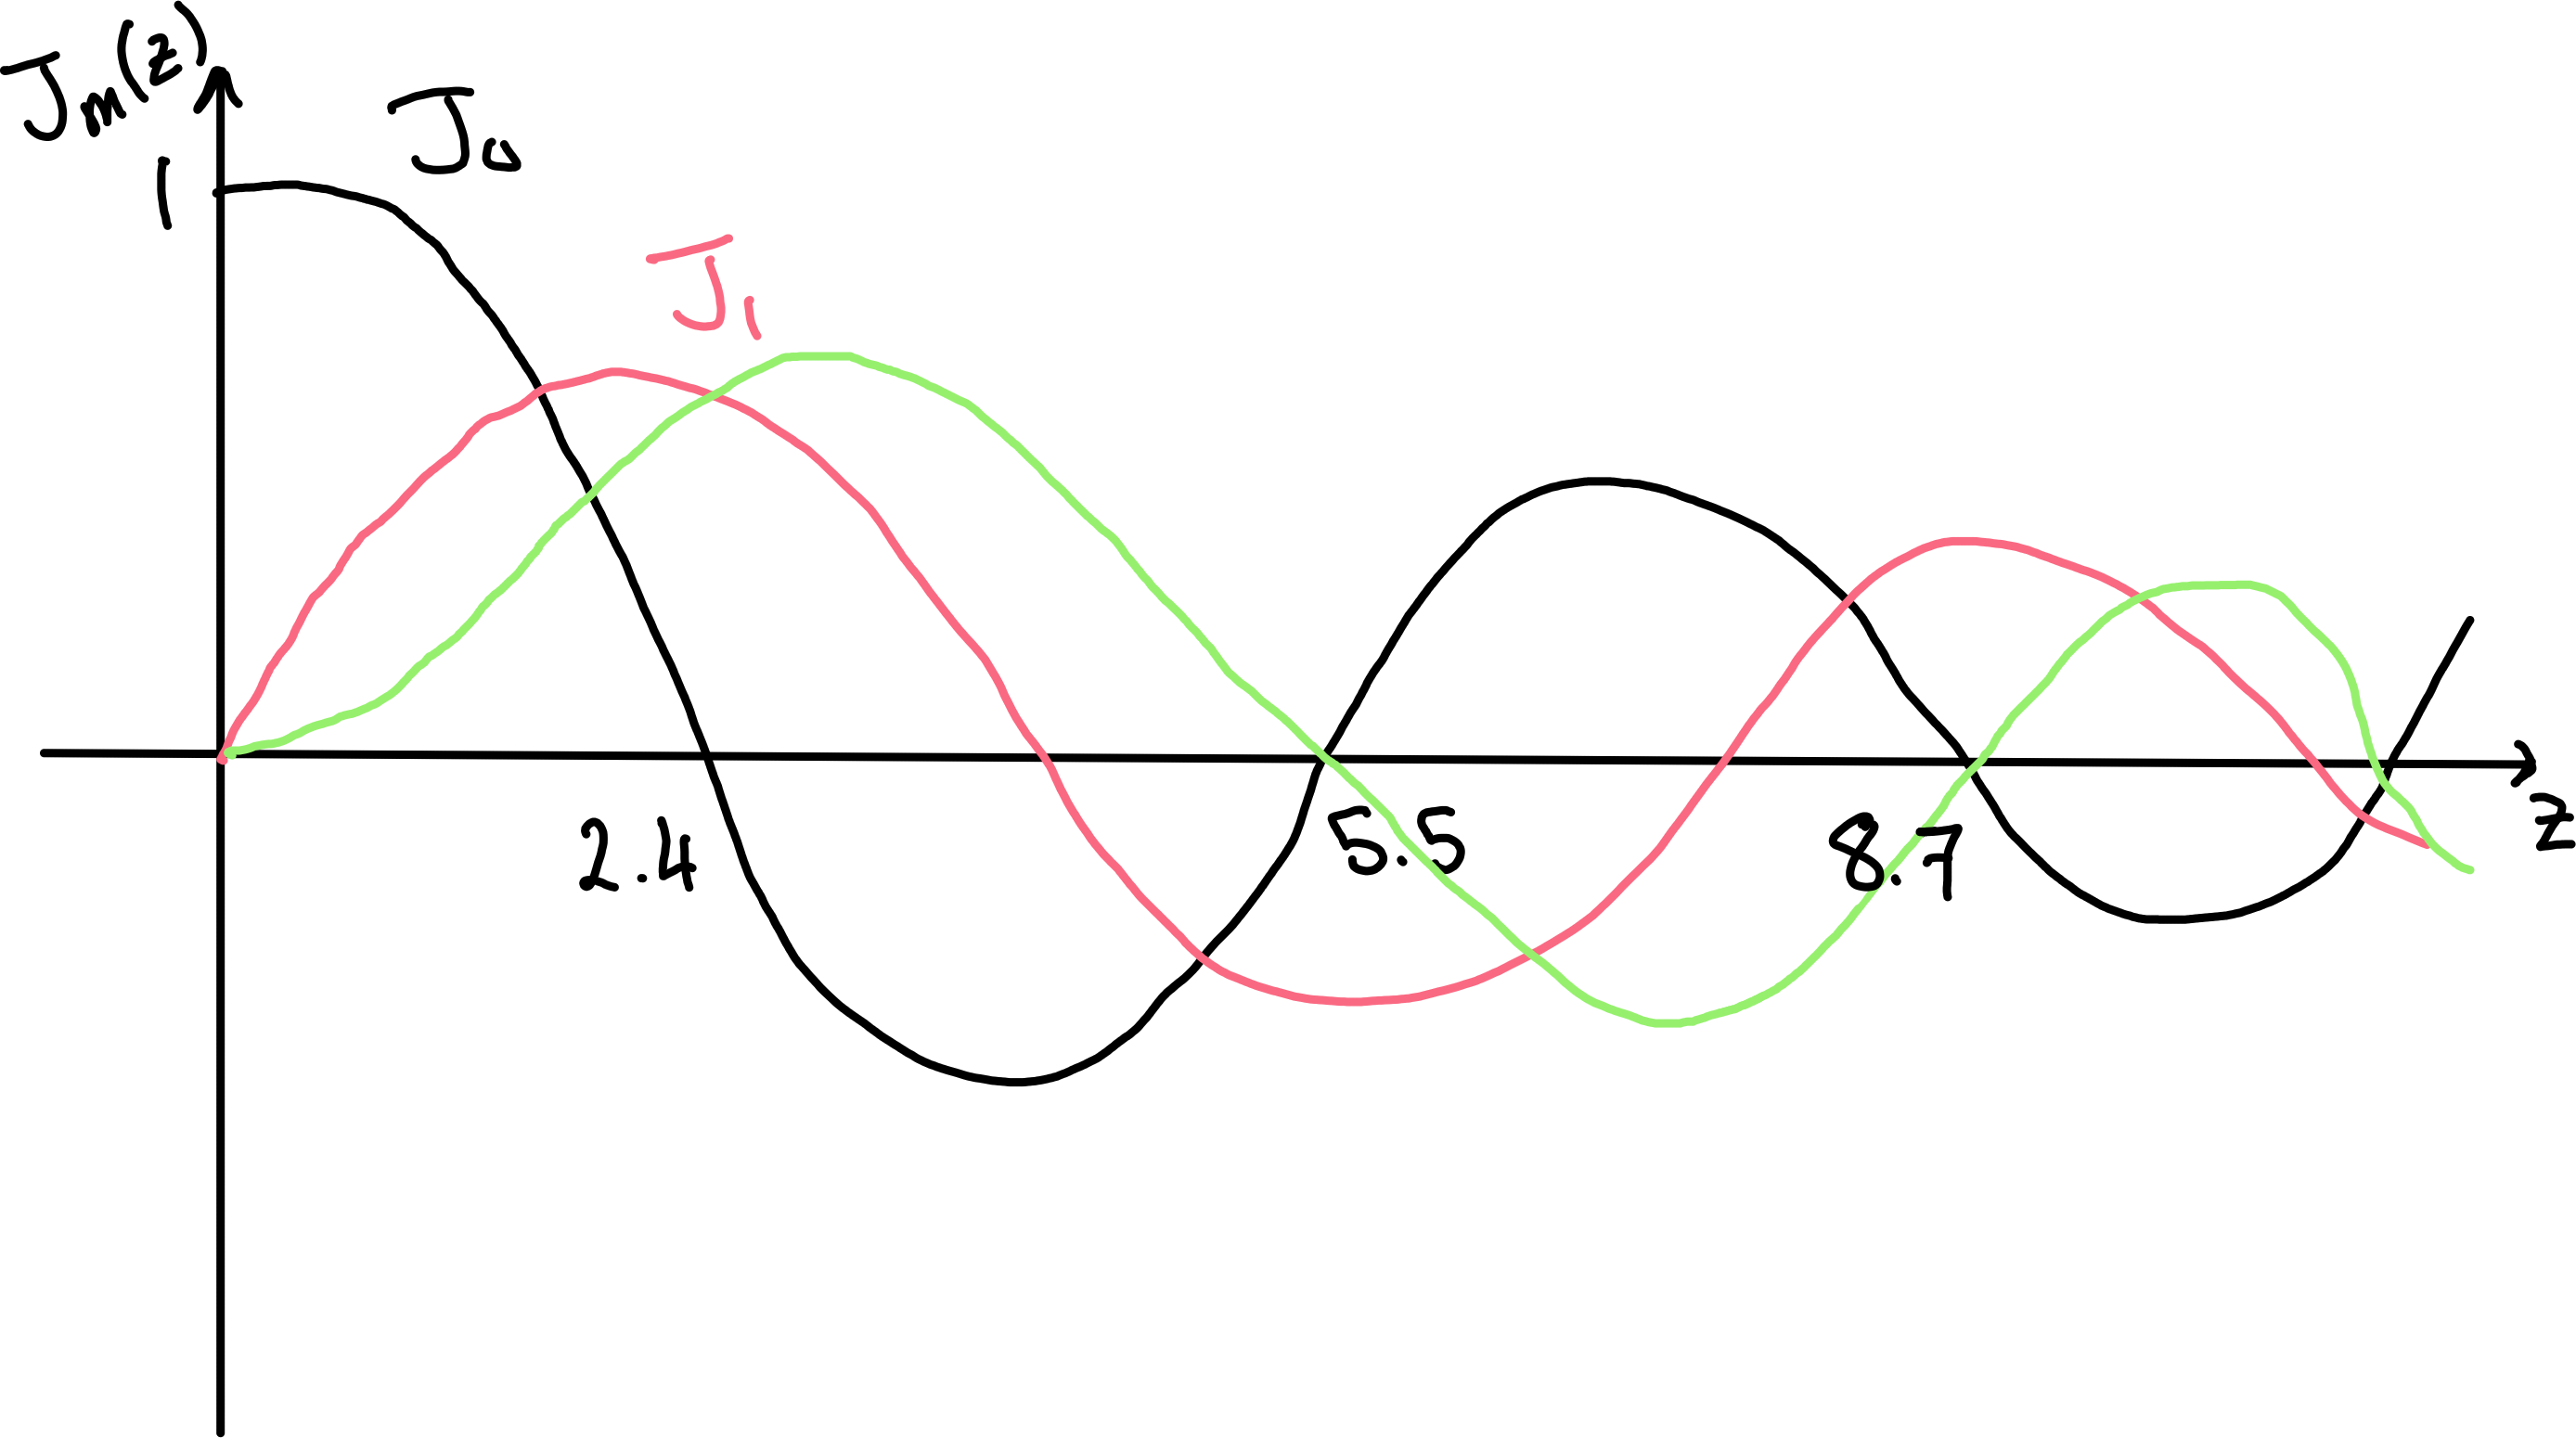
\includegraphics[height=5cm]{03-besselfunctions} 
\end{figure}

\subsection{Solving the vibrating drum}
Recall that the radial solutions to \cref{eq:3.26} become
\begin{align*}
	R_m(z) = R_m(\sqrt{\lambda} x) = A J_m(\sqrt{\lambda} x) + B Y_m(\sqrt{\lambda} x)
\end{align*}
Imposing the boundary condition of boundedness at $r = 0$, we must have $B = 0$ by \cref{eq:3.31}.
Further imposing $r = 1$ and $R = 0$ gives $J_m(\sqrt{\lambda}) = 0$.
These zeroes occur at $j_{mn} \approx n \pi + \frac{m \pi}{2} - \frac{\pi}{4}$.
Hence, the eigenvalues must be 
\begin{align} \label{eq:3.34}
	\lambda = j^2_{mn}.
\end{align}
Therefore, the spatial solution with the polar mode \cref{eq:3.26} is
\begin{align}
	V_{mn}(r, \theta) &= \Theta_m(\theta) R_{mn}(\sqrt{\lambda_{mn}} r) \notag \\
	&= (A_{mn} \cos m \theta + B_{mn} \sin m \theta) J_m (j_{mn} r) \label{eq:3.35}
\end{align}

The temporal solution \cref{eq:3.21} is
\begin{align*}
	\ddot T = -\lambda c^2 T \implies T_{mn}(t) = \cos(j_{mn} ct), \sin(j_{mn} ct)
\end{align*}

Combining everything together, the full solution to \cref{eq:3.17} is
\begin{align}
	\begin{aligned} \label{eq:3.36}
		u(r,\theta,t) & = \sum_{n=1}^\infty J_0(j_{0n} r) \qty( A_{0n}\cos j_{0n}ct + C_{0n}\sin j_{0n}ct ) \\
		&+ \sum_{m=1}^\infty \sum_{n=1}^\infty J_m (j_{mn}r) \qty( A_{mn} \cos m \theta + B_{mn} \sin m\theta ) \cos j_{mn} ct \\
		&+ \sum_{m=1}^\infty \sum_{n=1}^\infty J_m (j_{mn}r) \qty( C_{mn} \cos m \theta + D_{mn} \sin m\theta ) \sin j_{mn} ct
	\end{aligned}
\end{align} 

Now, we impose the \underline{initial conditions} \cref{eq:3.19} at $t = 0$
\begin{align} \label{eq:3.37}
	u(r,\theta,0) = \phi(r,\theta) = \sum_{m=0}^\infty \sum_{n=1}^\infty J_m (j_{mn}r) \qty( A_{mn} \cos m \theta + B_{mn} \sin m\theta )
\end{align}
and
\begin{align*}
	\pdv{u}{t}\qty(r,\theta,0) = \psi(r,\theta) = \sum_{m=0}^\infty \sum_{n=1}^\infty j_{mn} c J_m (j_{mn}r) \qty( C_{mn} \cos m \theta + D_{mn} \sin m\theta )
\end{align*}
We need to find the coefficients by multiplying by $J_m, \cos, \sin$ and using the orthogonality relations (\cref{eq:1.1,eq:1.2,eq:1.3} and Sheet 1, Q8), which are
\begin{align}
	\int_0^1 J_m(j_{mn} r) J_m(j_{mk} r) r \dd{r} &= \frac{1}{2}\qty[J_m'(j_{mn})]^2 \delta_{nk} \label{eq:3.38} \\
	&= \frac{1}{2}\qty[J_{m+1}(j_{mn})]^2 \delta_{nk} \label{eq:3.39}
\end{align}
by using a recursion relation of the Bessel functions.
We can then integrate to obtain the coefficients $A_{mn}$.
\begin{align*}
	\int_0^{2\pi} \dd{\theta} \cos p\theta \int_0^1 r \dd{r} J_p(j_{pq} r) \phi(r,\theta) = \frac{\pi}{2}\qty[J_{p+1}(j_{pq})]^2 A_{pq}
\end{align*}
where the $\frac{\pi}{2}$ coefficient is $2\pi$ for $p = 0$.
\begin{exercise}
	Find the analogous results for the $B_{mn}, C_{mn}, D_{mn}$.
\end{exercise} 
 
\begin{example}
	Consider an initial radial profile $u(r,\theta,0) = \phi(r) = 1 - r^2$.
	Then, $m = 0, B_{mn} = 0$ for all $m$ and $A_{mn} = 0$ for all $m \neq n$.
	Then
	\begin{align*}
		\pdv{u}{t}\qty(r,0,0) = 0
	\end{align*}
	hence $C_{mn}, D_{mn} = 0$.
	We just now need to find
	\begin{align*}
		A_{0n} = \frac{2}{J_1(j_{0n})^2} \int_0^1 J_0(j_{0n}r)(1-r)^2 r\dd{r} = \frac{2}{J_1(j_{0n})^2} \frac{J_2(j_{0n})}{j_{0n}^2} \approx \frac{J_2(j_{0n})}{n} \text{ as } n \to \infty
	\end{align*}
	Proving this is left as an exercise using \cref{eq:3.29,eq:3.30}.
	Then the approximate solution is
	\begin{align*}
		u(r,\theta,t) = \sum_{n=1}^\infty A_{0n} J_0(j_{0n}r)\cos j_{0n} ct
	\end{align*}
	The fundamental frequency is $\omega_d = j_{01} c \frac{2}{d} \approx 4.8\frac{c}{d}$ where $d$ is the diameter of the drum.
	Comparing this to a string with length $d$, this has a fundamental frequency of $\omega_s = \frac{\pi c}{d} \approx 0.77 \omega_d$.
\end{example}
    \section{Diffusion equation}
\subsection{Diffusion equation derivation with Fourier's law}
Fourier's law for heat flow is
\begin{align} \label{eq:4.1}
	q = -k \grad{\theta}
\end{align}
where $q$ is the heat flux, $k$ the thermal conductivity and $\theta$ is the temperature.
In a volume $V$, the overall heat energy $Q$ is given by
\begin{align} \label{eq:4.2}
	Q = \int_V c_V \rho \theta \dd{V}
\end{align}
where $c_V$ is the specific heat of the material, $\rho$ is the mass density.
The rate of change due to heat flow is
\begin{align*}
	\dv{Q}{t} = \int_V c_V \rho \pdv{\theta}{t} \dd{V} \tag{$\ast$}
\end{align*}
We will integrate \cref{eq:4.1} over the surface $S = \partial V$, giving
\begin{align*}
	-\dv{Q}{t} = \int_S q \cdot \hat n \dd{S}
\end{align*}
The negative sign is due to the normals facing outwards.
This is exactly
\begin{align*}
	-\dv{Q}{t} = \int_S (-k \grad{\theta}) \cdot \hat n \dd{S} = \int_V -k \laplacian{\theta} \dd{V} \tag{$\dagger$}
\end{align*}
Equating these two forms (($\ast$) and ($\dagger$)) for $\dv{Q}{t}$, we find
\begin{align*}
	\int_V (c_V \rho \pdv{\theta}{t} - k \laplacian{\theta}) \dd{V} = 0
\end{align*}
Since $V$ was arbitrary, the integrand must be zero.
So we have
\begin{align*}
	\pdv{\theta}{t} - \frac{k}{c_V \rho} \laplacian{\theta} = 0
\end{align*}
Let $D = \frac{k}{c_V \rho}$ be the diffusion constant.
Then we have the diffusion equation
\begin{align} \label{eq:4.3}
	\pdv{\theta}{t} - D \laplacian{\theta} = 0
\end{align}

\subsection{Diffusion equation derivation with statistical dynamics}
We can derive this equation in another way, using statistical dynamics.
Gas particles diffuse by scattering every fixed time step $\Delta t$ with probability density function $p(\xi)$ of moving by a displacement $\xi$.
On average, we have
\begin{align*}
	\mathbb{E}[\xi] = \int p(\xi) \xi \dd{\xi} = 0
\end{align*}
since there is no bias the direction in which any given particle is travelling.
Suppose that the probability density function after $N\Delta t$ time is described by $P_{N \Delta t}(x)$.
Then, for the next time step,
\begin{align*}
	P_{(N+1)\Delta t}(x) = \int_{-\infty}^\infty p(\xi) P_{N \Delta t}(x - \xi) \dd{\xi}
\end{align*}
Using the Taylor expansion,
\begin{align*}
	P_{(N+1)\Delta t}(x) & \approx \int_{-\infty}^\infty p(\xi) \qty[P_{N \Delta t}(x) + P_{N \Delta t}'(x)(-\xi) + P_{N \Delta t}''(x)\frac{\xi^2}{2} + \cdots] \dd{\xi} \\
	& \approx P_{N \Delta t}(x) - P_{N \Delta t}'(x) \mathbb{E}[\xi] + P_{N \Delta t}''(x) \frac{\mathbb{E}[\xi^2]}{2} + \cdots \\
	& \approx P_{N \Delta t}(x) + P_{N \Delta t}''(x) \frac{\mathbb{E}[\xi^2]}{2} + \cdots
\end{align*}
since $\int p(\xi) \dd{\xi} = 1$.
Identifying $P_{N \Delta t}(x) = P(x, N\Delta t)$, we can write
\begin{align*}
	P(x, (N+1)\Delta t) - P(x, N \Delta t) = \pdv[2]{x} P(x, N\Delta t) \frac{\mathbb{E}[\xi^2]}{2}
\end{align*}
Assuming that the variance $\mathbb{E}[\xi^2]$\footnote{$\Var X = \mathbb{E}[X^2] - \mathbb{E}[X]^2$ and $\mathbb{E}[X] = 0$.} is equal to $2D \Delta t$, then for small $\Delta t$, we find
\begin{align} \label{eq:4.4}
	\pdv{P}{t} = D \pdv[2]{P}{x}
\end{align}
which is exactly the diffusion equation.

\subsection{Similarity solutions}
The characteristic relation between the variance and time suggests that we seek solutions with a dimensionless parameter.
If we can find a change of variables of the form $\theta(\eta) = \theta(x,t)$, then it will likely be easier to solve.
Consider
\begin{align} \label{eq:4.5}
	\eta \equiv \frac{x}{2\sqrt{Dt}}
\end{align}
Then changing variables in \cref{eq:4.3},
\begin{align*}
	\pdv{\theta}{t} = \pdv{\eta}{t} \pdv{\theta}{\eta} = \frac{-1}{2} \frac{x}{\sqrt{D} t^{3/2}} \theta' = \frac{-1}{2} \frac{\eta}{t} \theta'
\end{align*}
and
\begin{align*}
	D \pdv[2]{\theta}{x} = D \pdv{x} \qty(\pdv{\eta}{x} \pdv{\theta}{\eta}) = D \pdv{x} \qty(\frac{1}{2\sqrt{Dt}} \theta') = \frac{D}{4Dt} \theta'' = \frac{1}{4t} \theta''
\end{align*}
Equating,
\begin{align} \label{eq:4.6}
	\theta'' = -2 \eta \theta'
\end{align}
Let $\psi = \theta'$.
Then
\begin{align*}
	\frac{\psi'}{\psi} = -2\eta \implies \ln \psi = -\eta^2 + \text{constant}
\end{align*}
Then, choosing a constant of $c\frac{2}{\sqrt{\pi}}$,
\begin{align} \label{eq:4.7}
	\psi = c\frac{2}{\sqrt{\pi}} e^{-\eta^2} \implies \theta(\eta) = c\frac{2}{\sqrt{\pi}} \int_0^\eta e^{-u^2} \dd{u} = c \erf(\eta) = c \erf \qty(\frac{x}{2\sqrt{Dt}})
\end{align}
where
\begin{align*}
	\erf(z) = \frac{2}{\sqrt{\pi}} \int_0^z e^{-u^2} \dd{u}
\end{align*}
This describes discontinuous initial conditions that spread over time.

\begingroup
\tikzset{every picture/.style={scale=1}}
% Recommended preamble:
% \usetikzlibrary{arrows.meta}
% \usetikzlibrary{backgrounds}
% \usepgfplotslibrary{patchplots}
% \usepgfplotslibrary{fillbetween}
% \pgfplotsset{%
%     layers/standard/.define layer set={%
%         background,axis background,axis grid,axis ticks,axis lines,axis tick labels,pre main,main,axis descriptions,axis foreground%
%     }{
%         grid style={/pgfplots/on layer=axis grid},%
%         tick style={/pgfplots/on layer=axis ticks},%
%         axis line style={/pgfplots/on layer=axis lines},%
%         label style={/pgfplots/on layer=axis descriptions},%
%         legend style={/pgfplots/on layer=axis descriptions},%
%         title style={/pgfplots/on layer=axis descriptions},%
%         colorbar style={/pgfplots/on layer=axis descriptions},%
%         ticklabel style={/pgfplots/on layer=axis tick labels},%
%         axis background@ style={/pgfplots/on layer=axis background},%
%         3d box foreground style={/pgfplots/on layer=axis foreground},%
%     },
% }

\begin{tikzpicture}[/tikz/background rectangle/.style={fill={rgb,1:red,1.0;green,1.0;blue,1.0}, draw opacity={1.0}}, show background rectangle]
\begin{axis}[point meta max={nan}, point meta min={nan}, legend cell align={left}, legend columns={1}, title={$D=1$}, title style={at={{(0.5,1)}}, anchor={south}, font={{\fontsize{14 pt}{18.2 pt}\selectfont}}, color={rgb,1:red,0.0;green,0.0;blue,0.0}, draw opacity={1.0}, rotate={0.0}, align={center}}, legend style={color={rgb,1:red,0.0;green,0.0;blue,0.0}, draw opacity={1.0}, line width={1}, solid, fill={rgb,1:red,1.0;green,1.0;blue,1.0}, fill opacity={1.0}, text opacity={1.0}, font={{\fontsize{8 pt}{10.4 pt}\selectfont}}, text={rgb,1:red,0.0;green,0.0;blue,0.0}, cells={anchor={center}}, at={(1.02, 1)}, anchor={north west}}, axis background/.style={fill={rgb,1:red,1.0;green,1.0;blue,1.0}, opacity={1.0}}, anchor={north west}, xshift={1.0mm}, yshift={-1.0mm}, width={145.4mm}, height={99.6mm}, scaled x ticks={false}, xlabel={$x$}, x tick style={color={rgb,1:red,0.0;green,0.0;blue,0.0}, opacity={1.0}}, x tick label style={color={rgb,1:red,0.0;green,0.0;blue,0.0}, opacity={1.0}, rotate={0}}, xlabel style={at={(ticklabel cs:0.5)}, anchor=near ticklabel, at={{(ticklabel cs:0.5)}}, anchor={near ticklabel}, font={{\fontsize{11 pt}{14.3 pt}\selectfont}}, color={rgb,1:red,0.0;green,0.0;blue,0.0}, draw opacity={1.0}, rotate={0.0}}, xmajorgrids={true}, xmin={-3.18}, xmax={3.18}, xticklabels={{$-3$,$-2$,$-1$,$0$,$1$,$2$,$3$}}, xtick={{-3.0,-2.0,-1.0,0.0,1.0,2.0,3.0}}, xtick align={inside}, xticklabel style={font={{\fontsize{8 pt}{10.4 pt}\selectfont}}, color={rgb,1:red,0.0;green,0.0;blue,0.0}, draw opacity={1.0}, rotate={0.0}}, x grid style={color={rgb,1:red,0.0;green,0.0;blue,0.0}, draw opacity={0.1}, line width={0.5}, solid}, axis x line*={left}, x axis line style={color={rgb,1:red,0.0;green,0.0;blue,0.0}, draw opacity={1.0}, line width={1}, solid}, scaled y ticks={false}, ylabel={$\theta$}, y tick style={color={rgb,1:red,0.0;green,0.0;blue,0.0}, opacity={1.0}}, y tick label style={color={rgb,1:red,0.0;green,0.0;blue,0.0}, opacity={1.0}, rotate={0}}, ylabel style={at={(ticklabel cs:0.5)}, anchor=near ticklabel, at={{(ticklabel cs:0.5)}}, anchor={near ticklabel}, font={{\fontsize{11 pt}{14.3 pt}\selectfont}}, color={rgb,1:red,0.0;green,0.0;blue,0.0}, draw opacity={1.0}, rotate={0.0}}, ymajorgrids={true}, ymin={-1.06}, ymax={1.06}, yticklabels={{$-1.0$,$-0.5$,$0.0$,$0.5$,$1.0$}}, ytick={{-1.0,-0.5,0.0,0.5,1.0}}, ytick align={inside}, yticklabel style={font={{\fontsize{8 pt}{10.4 pt}\selectfont}}, color={rgb,1:red,0.0;green,0.0;blue,0.0}, draw opacity={1.0}, rotate={0.0}}, y grid style={color={rgb,1:red,0.0;green,0.0;blue,0.0}, draw opacity={0.1}, line width={0.5}, solid}, axis y line*={left}, y axis line style={color={rgb,1:red,0.0;green,0.0;blue,0.0}, draw opacity={1.0}, line width={1}, solid}, colorbar={false}]
    \addplot[color={rgb,1:red,0.0;green,0.6056;blue,0.9787}, name path={bbbde1b4-bfdc-4bb8-9cd6-47f3119a67c6}, draw opacity={1.0}, line width={1}, solid]
        table[row sep={\\}]
        {
            \\
            -3.0  -1.0  \\
            -2.9609367239208475  -1.0  \\
            -2.5997403313265086  -1.0  \\
            -2.3826763547775043  -1.0  \\
            -2.199151525136937  -1.0  \\
            -1.9997921198677944  -1.0  \\
            -1.8160003818614874  -1.0  \\
            -1.6189562143740408  -1.0  \\
            -1.3906612226458708  -1.0  \\
            -1.1877795755559142  -1.0  \\
            -1.00987065383912  -1.0  \\
            -0.8159021733787222  -1.0  \\
            -0.6207808849887516  -1.0  \\
            -0.5129151172455673  -1.0  \\
            -0.40504934950238297  -1.0  \\
            -0.30241779326150453  -1.0  \\
            -0.19978623702062615  -1.0  \\
            -0.14642973425411906  -1.0  \\
            -0.093073231487612  -1.0  \\
            -0.06639498010435846  -1.0  \\
            -0.03971672872110493  -1.0  \\
            -0.03304716587529155  -1.0  \\
            -0.026377603029478166  -1.0  \\
            -0.01970804018366478  -1.0  \\
            -0.0130384773378514  -1.0  \\
            -0.009703695914944709  -1.0  \\
            -0.006368914492038016  -1.0  \\
            -0.00470152378058467  -1.0  \\
            -0.003034133069131324  -1.0  \\
            -0.001366742357677978  -1.0  \\
            0.0003006483537753681  1.0  \\
            0.0019680390652287143  1.0  \\
            0.00363542977668206  1.0  \\
            0.005302820488135406  1.0  \\
            0.006970211199588752  1.0  \\
            0.010304992622495443  1.0  \\
            0.013639774045402136  1.0  \\
            0.02486847658427578  1.0  \\
            0.03609717912314943  1.0  \\
            0.047325881662023075  1.0  \\
            0.05855458420089672  1.0  \\
            0.08101198927864402  1.0  \\
            0.10346939435639131  1.0  \\
            0.1483842045118859  1.0  \\
            0.19329901466738048  1.0  \\
            0.41264258394545644  1.0  \\
            0.6135751697836116  1.0  \\
            0.7991519189555105  1.0  \\
            0.9871354150600441  1.0  \\
            1.1978122140406555  1.0  \\
            1.388719406219134  1.0  \\
            1.6072949743767582  1.0  \\
            1.8096765128752679  1.0  \\
            2.009200994923107  1.0  \\
            2.202922753671847  1.0  \\
            2.4015123274889874  1.0  \\
            2.6190902607646405  1.0  \\
            2.93515789239279  1.0  \\
            3.0  1.0  \\
        }
        ;
    \addlegendentry {$t=0$}
    \addplot[color={rgb,1:red,0.8889;green,0.4356;blue,0.2781}, name path={59314d39-cec7-4ae5-9cca-64005a7635a4}, draw opacity={1.0}, line width={1}, solid]
        table[row sep={\\}]
        {
            \\
            -3.0  -1.0  \\
            -2.9609367239208475  -1.0  \\
            -2.5997403313265086  -1.0  \\
            -2.3826763547775043  -1.0  \\
            -2.199151525136937  -1.0  \\
            -1.9997921198677944  -1.0  \\
            -1.8160003818614874  -1.0  \\
            -1.6189562143740408  -1.0  \\
            -1.3906612226458708  -1.0  \\
            -1.1877795755559142  -1.0  \\
            -1.00987065383912  -1.0  \\
            -0.8159021733787222  -1.0  \\
            -0.6207808849887516  -1.0  \\
            -0.5129151172455673  -1.0  \\
            -0.40504934950238297  -1.0  \\
            -0.3537335713819437  -0.9999999999999974  \\
            -0.30241779326150453  -0.9999999999864151  \\
            -0.25110201514106534  -0.9999999803223646  \\
            -0.19978623702062615  -0.9999920807742605  \\
            -0.17310798563737262  -0.9998915266778654  \\
            -0.14642973425411906  -0.9989406406086226  \\
            -0.1330906085624923  -0.9970796178516699  \\
            -0.11975148287086554  -0.992587585404849  \\
            -0.11308192002505216  -0.9885477823344052  \\
            -0.10641235717923878  -0.9826616292816677  \\
            -0.0997427943334254  -0.9742735736645938  \\
            -0.093073231487612  -0.9625826328591867  \\
            -0.0897384500647053  -0.9552090868523828  \\
            -0.0864036686417986  -0.9466460192128695  \\
            -0.08306888721889191  -0.9367566491563639  \\
            -0.07973410579598522  -0.9253988507524387  \\
            -0.07639932437307853  -0.9124268801068293  \\
            -0.07306454295017184  -0.8976934443929281  \\
            -0.06972976152726515  -0.8810521010229675  \\
            -0.06639498010435846  -0.8623599618888228  \\
            -0.06306019868145177  -0.8414806634259511  \\
            -0.05972541725854508  -0.8182875488181677  \\
            -0.056390635835638386  -0.7926669946093696  \\
            -0.053055854412731696  -0.7645218010252804  \\
            -0.049721072989825005  -0.7337745541652834  \\
            -0.046386291566918314  -0.7003708596205451  \\
            -0.04305151014401162  -0.6642823416736524  \\
            -0.03971672872110493  -0.6255093006010505  \\
            -0.03638194729819824  -0.5840829231549527  \\
            -0.03304716587529155  -0.5400669482891236  \\
            -0.02971238445238486  -0.49355870164745336  \\
            -0.026377603029478166  -0.4446894280627415  \\
            -0.02304282160657147  -0.39362387088969103  \\
            -0.01970804018366478  -0.3405590697701961  \\
            -0.01637325876075809  -0.2857223735481934  \\
            -0.0130384773378514  -0.22936869149833367  \\
            -0.006368914492038016  -0.11324640882870098  \\
            0.0003006483537753681  0.0053638993811737316  \\
            0.006970211199588752  0.12385556892554953  \\
            0.013639774045402136  0.23962974986643085  \\
            0.016446949680120546  0.286951512666272  \\
            0.019254125314838957  0.3331937279503094  \\
            0.02206130094955737  0.37820338860902075  \\
            0.02486847658427578  0.42184112721921957  \\
            0.027675652218994193  0.46398244623814067  \\
            0.030482827853712605  0.5045186807337945  \\
            0.033290003488431016  0.5433576837155185  \\
            0.03609717912314943  0.5804242308842567  \\
            0.03890435475786784  0.6156601482194205  \\
            0.04171153039258625  0.6490241720614864  \\
            0.044518706027304664  0.6804915570600641  \\
            0.047325881662023075  0.7100534523854313  \\
            0.05013305729674149  0.7377160708274008  \\
            0.0529402329314599  0.7634996787425251  \\
            0.05574740856617831  0.7874374372078601  \\
            0.05855458420089672  0.8095741261807469  \\
            0.061361759835615134  0.8299647839669007  \\
            0.06416893547033355  0.8486732939118713  \\
            0.06697611110505196  0.8657709490289307  \\
            0.06978328673977037  0.8813350233570115  \\
            0.07259046237448878  0.8954473763196841  \\
            0.0753976380092072  0.9081931133556759  \\
            0.0782048136439256  0.9196593227441014  \\
            0.08101198927864402  0.9299339049845103  \\
            0.08662634054808084  0.9472575733238839  \\
            0.09224069181751766  0.9608459833298386  \\
            0.09785504308695449  0.9713380658048624  \\
            0.10346939435639131  0.9793128514223746  \\
            0.10908374562582812  0.9852796393459977  \\
            0.11469809689526494  0.9896743111476254  \\
            0.12031244816470177  0.9928605369310586  \\
            0.1259267994341386  0.9951345392296561  \\
            0.13715550197301224  0.9978370174858159  \\
            0.1483842045118859  0.9990932632288029  \\
            0.17084160958963318  0.9998666210921499  \\
            0.19329901466738048  0.9999845587122477  \\
            0.24813490698689947  0.9999999711811763  \\
            0.30297079930641846  0.9999999999875278  \\
            0.3578066916259375  0.9999999999999988  \\
            0.41264258394545644  1.0  \\
            0.513108876864534  1.0  \\
            0.6135751697836116  1.0  \\
            0.7991519189555105  1.0  \\
            0.9871354150600441  1.0  \\
            1.1978122140406555  1.0  \\
            1.388719406219134  1.0  \\
            1.6072949743767582  1.0  \\
            1.8096765128752679  1.0  \\
            2.009200994923107  1.0  \\
            2.202922753671847  1.0  \\
            2.4015123274889874  1.0  \\
            2.6190902607646405  1.0  \\
            2.93515789239279  1.0  \\
            3.0  1.0  \\
        }
        ;
    \addlegendentry {$t = 10^{-3}$}
    \addplot[color={rgb,1:red,0.2422;green,0.6433;blue,0.3044}, name path={6232a22f-da1a-4c5f-bc6f-625fd2918cd1}, draw opacity={1.0}, line width={1}, solid]
        table[row sep={\\}]
        {
            \\
            -3.0  -1.0  \\
            -2.9609367239208475  -1.0  \\
            -2.5997403313265086  -1.0  \\
            -2.3826763547775043  -1.0  \\
            -2.199151525136937  -1.0  \\
            -1.9997921198677944  -1.0  \\
            -1.8160003818614874  -1.0  \\
            -1.6189562143740408  -1.0  \\
            -1.3906612226458708  -1.0  \\
            -1.1877795755559142  -1.0  \\
            -1.00987065383912  -0.9999999999990725  \\
            -0.8159021733787222  -0.9999999920398323  \\
            -0.6207808849887516  -0.999988643215685  \\
            -0.5668480011171595  -0.9999388220531092  \\
            -0.5129151172455673  -0.9997131085680446  \\
            -0.45898223337397515  -0.9988275316927056  \\
            -0.40504934950238297  -0.9958184551343818  \\
            -0.3793914604421633  -0.9926970129518808  \\
            -0.3537335713819437  -0.9876252628633458  \\
            -0.3280756823217241  -0.9796507577343972  \\
            -0.30241779326150453  -0.9675170636513158  \\
            -0.28958884873139473  -0.9594108301709481  \\
            -0.27675990420128493  -0.9496511266833726  \\
            -0.26393095967117514  -0.9379969194652074  \\
            -0.25110201514106534  -0.9241944293155557  \\
            -0.23827307061095554  -0.9079815274514302  \\
            -0.22544412608084574  -0.8890932366540245  \\
            -0.21261518155073594  -0.8672682912771007  \\
            -0.19978623702062615  -0.8422566454994204  \\
            -0.18644711132899938  -0.8126235835725499  \\
            -0.17310798563737262  -0.7790697666197243  \\
            -0.15976885994574586  -0.7414127036366686  \\
            -0.14642973425411906  -0.6995246606893336  \\
            -0.1330906085624923  -0.6533426531858829  \\
            -0.11975148287086554  -0.6028771442900945  \\
            -0.10641235717923878  -0.5482189073424177  \\
            -0.093073231487612  -0.4895435567034366  \\
            -0.07973410579598522  -0.4271133344608578  \\
            -0.06639498010435846  -0.36127585721187666  \\
            -0.053055854412731696  -0.2924596718988572  \\
            -0.03971672872110493  -0.22116663394829106  \\
            -0.0130384773378514  -0.07345765012125084  \\
            0.013639774045402136  0.07683504383068354  \\
            0.03609717912314943  0.20146658764768505  \\
            0.05855458420089672  0.3211577031628891  \\
            0.06978328673977037  0.37829993705741255  \\
            0.08101198927864402  0.43324782699217496  \\
            0.09224069181751766  0.48575376102908213  \\
            0.10346939435639131  0.5356111259612224  \\
            0.11469809689526494  0.582656163336171  \\
            0.1259267994341386  0.6267686843337225  \\
            0.13715550197301224  0.6678716825237805  \\
            0.1483842045118859  0.7059299215437114  \\
            0.15961290705075953  0.7409476072284354  \\
            0.17084160958963318  0.7729652794710861  \\
            0.18207031212850683  0.8020560773038202  \\
            0.19329901466738048  0.8283215410471984  \\
            0.20700798774726023  0.8567425199211242  \\
            0.22071696082713999  0.8814065339278863  \\
            0.2344259339070197  0.9026101874489814  \\
            0.24813490698689947  0.9206686117630558  \\
            0.2618438800667792  0.935904620771657  \\
            0.27555285314665895  0.9486392058987063  \\
            0.28926182622653873  0.9591835748376183  \\
            0.30297079930641846  0.9678328277587064  \\
            0.33038874546617797  0.980519243423162  \\
            0.3578066916259375  0.9885961976222444  \\
            0.38522463778569693  0.9935493638073194  \\
            0.41264258394545644  0.9964751641207977  \\
            0.4628757304049952  0.9989359718937953  \\
            0.513108876864534  0.9997146264359955  \\
            0.5633420233240728  0.999932072213213  \\
            0.6135751697836116  0.9999856627398552  \\
            0.7991519189555105  0.9999999840350515  \\
            0.9871354150600441  0.9999999999970504  \\
            1.1978122140406555  1.0  \\
            1.388719406219134  1.0  \\
            1.6072949743767582  1.0  \\
            1.8096765128752679  1.0  \\
            2.009200994923107  1.0  \\
            2.202922753671847  1.0  \\
            2.4015123274889874  1.0  \\
            2.6190902607646405  1.0  \\
            2.93515789239279  1.0  \\
            3.0  1.0  \\
        }
        ;
    \addlegendentry {$t = 10^{-2}$}
    \addplot[color={rgb,1:red,0.7644;green,0.4441;blue,0.8243}, name path={5b059462-f580-4bc3-927d-d091966c8ddf}, draw opacity={1.0}, line width={1}, solid]
        table[row sep={\\}]
        {
            \\
            -3.0  -0.9999999999802965  \\
            -2.9609367239208475  -0.9999999999642875  \\
            -2.5997403313265086  -0.9999999938708811  \\
            -2.3826763547775043  -0.9999999006048895  \\
            -2.199151525136937  -0.9999991232218955  \\
            -1.9997921198677944  -0.9999922389279503  \\
            -1.8160003818614874  -0.9999510742576445  \\
            -1.6189562143740408  -0.9997055064352888  \\
            -1.3906612226458708  -0.9981266740459626  \\
            -1.2892203991008926  -0.996058229330461  \\
            -1.1877795755559142  -0.9920916038051636  \\
            -1.098825114697517  -0.98599158960537  \\
            -1.00987065383912  -0.9760630319759493  \\
            -0.9613785337240206  -0.9684216612329685  \\
            -0.9128864136089211  -0.9587766063969309  \\
            -0.8643942934938216  -0.9467446310665077  \\
            -0.8159021733787222  -0.9319102999877525  \\
            -0.7671218512812296  -0.9137164692541145  \\
            -0.718341529183737  -0.8917833125426629  \\
            -0.6695612070862442  -0.8656547099010363  \\
            -0.6207808849887516  -0.8348959176479536  \\
            -0.5938144430529555  -0.815758939248996  \\
            -0.5668480011171595  -0.7950272468173949  \\
            -0.5398815591813634  -0.7726494382101249  \\
            -0.5129151172455673  -0.7485824491553721  \\
            -0.4859486753097712  -0.7227926848408014  \\
            -0.45898223337397515  -0.6952570943935861  \\
            -0.43201579143817903  -0.6659641638905588  \\
            -0.40504934950238297  -0.6349148036285647  \\
            -0.3793914604421633  -0.6037541899450509  \\
            -0.3537335713819437  -0.5710398508393102  \\
            -0.3280756823217241  -0.5368071509610597  \\
            -0.30241779326150453  -0.5011033044668204  \\
            -0.27675990420128493  -0.4639874286318324  \\
            -0.25110201514106534  -0.42553044013826347  \\
            -0.22544412608084574  -0.3858147892936949  \\
            -0.19978623702062615  -0.3449340304976142  \\
            -0.14642973425411906  -0.25665493091768976  \\
            -0.093073231487612  -0.1648632237043389  \\
            -0.03971672872110493  -0.0707665376161081  \\
            0.013639774045402136  0.02433127752607976  \\
            0.05855458420089672  0.10417092401891336  \\
            0.10346939435639131  0.18296843529616683  \\
            0.1483842045118859  0.25995757718556245  \\
            0.19329901466738048  0.33442555133647794  \\
            0.22071696082713999  0.3783675939685244  \\
            0.24813490698689947  0.42100035518126816  \\
            0.27555285314665895  0.46220771620717255  \\
            0.30297079930641846  0.5018879538003761  \\
            0.33038874546617797  0.5399543571937845  \\
            0.3578066916259375  0.5763356014049799  \\
            0.38522463778569693  0.6109758794934395  \\
            0.41264258394545644  0.6438348015677368  \\
            0.43775915717522584  0.6723504624507537  \\
            0.4628757304049952  0.6993411753293457  \\
            0.4879923036347646  0.7248080571352101  \\
            0.513108876864534  0.7487614861836827  \\
            0.5382254500943033  0.7712204708068556  \\
            0.5633420233240728  0.7922119501280058  \\
            0.5884585965538423  0.8117700417603212  \\
            0.6135751697836116  0.8299352512613053  \\
            0.6599693570765863  0.8599853151462249  \\
            0.7063635443695611  0.8857732895562674  \\
            0.7527577316625358  0.9076669977091159  \\
            0.7991519189555105  0.9260557253674235  \\
            0.8461477929816439  0.9415148792772384  \\
            0.8931436670077773  0.9541889321493429  \\
            0.9401395410339106  0.9644656343181565  \\
            0.9871354150600441  0.9727070247171536  \\
            1.039804614805197  0.9799319857760929  \\
            1.0924738145503499  0.9854280345188169  \\
            1.1451430142955026  0.9895513713318527  \\
            1.1978122140406555  0.9926022870830888  \\
            1.2932658101298946  0.9961699519476673  \\
            1.388719406219134  0.9980989523433339  \\
            1.6072949743767582  0.9996743862024866  \\
            1.8096765128752679  0.9999480241265823  \\
            2.009200994923107  0.9999929677484587  \\
            2.202922753671847  0.999999160206309  \\
            2.4015123274889874  0.9999999212392595  \\
            2.6190902607646405  0.9999999952717359  \\
            2.93515789239279  0.9999999999473393  \\
            3.0  0.9999999999802965  \\
        }
        ;
    \addlegendentry {$t = 10^{-1}$}
    \addplot[color={rgb,1:red,0.6755;green,0.5557;blue,0.0942}, name path={0cf45548-f4cb-4113-812c-0099f95a8aac}, draw opacity={1.0}, line width={1}, solid]
        table[row sep={\\}]
        {
            \\
            -3.0  -0.9661051464753108  \\
            -2.9804683619604235  -0.9649265513695182  \\
            -2.9609367239208475  -0.9637131476610028  \\
            -2.780338527623678  -0.9507009535411899  \\
            -2.5997403313265086  -0.9339809078317416  \\
            -2.4912083430520067  -0.9218546947755499  \\
            -2.3826763547775043  -0.9079741103736406  \\
            -2.2909139399572207  -0.8947507050232054  \\
            -2.199151525136937  -0.8800622557069969  \\
            -2.0994718225023656  -0.8623371333225704  \\
            -1.9997921198677944  -0.8426576421642085  \\
            -1.9078962508646409  -0.8226907765011833  \\
            -1.8160003818614874  -0.800895195630151  \\
            -1.717478298117764  -0.7754204617158442  \\
            -1.6189562143740408  -0.7476975919364297  \\
            -1.5048087185099557  -0.7126986837363251  \\
            -1.3906612226458708  -0.6745628129799148  \\
            -1.2892203991008926  -0.6380293595393353  \\
            -1.1877795755559142  -0.5990282485263874  \\
            -1.098825114697517  -0.5628333768753401  \\
            -1.00987065383912  -0.5248262371810903  \\
            -0.9128864136089211  -0.4814020767489276  \\
            -0.8159021733787222  -0.4360132290296584  \\
            -0.718341529183737  -0.3885075003436815  \\
            -0.6207808849887516  -0.33930830126002426  \\
            -0.40504934950238297  -0.22543828953726075  \\
            -0.19978623702062615  -0.11234351191459552  \\
            0.013639774045402136  0.007695299133184976  \\
            0.19329901466738048  0.10871866739332182  \\
            0.41264258394545644  0.22954697379827776  \\
            0.6135751697836116  0.3356121891295767  \\
            0.7063635443695611  0.3825548196293288  \\
            0.7991519189555105  0.42798455343073566  \\
            0.8931436670077773  0.47231768843832095  \\
            0.9871354150600441  0.5148291509948483  \\
            1.0924738145503499  0.560179073273832  \\
            1.1978122140406555  0.6029943656709459  \\
            1.2932658101298946  0.6395337547604393  \\
            1.388719406219134  0.6738868053395398  \\
            1.4980071902979462  0.7105145352535559  \\
            1.6072949743767582  0.7442648378289973  \\
            1.708485743626013  0.7729842215155165  \\
            1.8096765128752679  0.7993263015146979  \\
            1.9094387538991873  0.823040815268532  \\
            2.009200994923107  0.8446017218668409  \\
            2.106061874297477  0.8635680882796628  \\
            2.202922753671847  0.8806960031086348  \\
            2.3022175405804175  0.896456800101484  \\
            2.4015123274889874  0.9105159509688344  \\
            2.5103012941268137  0.924110544584302  \\
            2.6190902607646405  0.9359708001764229  \\
            2.7771240765787155  0.9504378071140105  \\
            2.93515789239279  0.9620570081267613  \\
            2.967578946196395  0.9641297507378738  \\
            3.0  0.9661051464753108  \\
        }
        ;
    \addlegendentry {$t = 10^{0}$}
    \addplot[color={rgb,1:red,0.0;green,0.6658;blue,0.681}, name path={6c348c63-e572-40ab-ad16-8281c07017b0}, draw opacity={1.0}, line width={1}, solid]
        table[row sep={\\}]
        {
            \\
            -3.0  -0.4976650456394979  \\
            -2.9609367239208475  -0.4920836227218486  \\
            -2.5997403313265086  -0.43897493384921343  \\
            -2.3826763547775043  -0.40581594060647647  \\
            -2.199151525136937  -0.377100540780792  \\
            -1.9997921198677944  -0.3452455946644038  \\
            -1.8160003818614874  -0.3153088542753728  \\
            -1.6189562143740408  -0.28265515450352807  \\
            -1.3906612226458708  -0.24416995989970192  \\
            -1.1877795755559142  -0.20944931561484767  \\
            -1.00987065383912  -0.1786538678263862  \\
            -0.8159021733787222  -0.1447635613129309  \\
            -0.6207808849887516  -0.11040036093870902  \\
            -0.40504934950238297  -0.07216715029243596  \\
            -0.19978623702062615  -0.03563249183921455  \\
            0.013639774045402136  0.0024335012085193544  \\
            0.19329901466738048  0.0344762081473073  \\
            0.41264258394545644  0.07351622797628538  \\
            0.6135751697836116  0.10912695624295243  \\
            0.7991519189555105  0.14182343396963817  \\
            0.9871354150600441  0.17469747633775828  \\
            1.1978122140406555  0.21117671475710043  \\
            1.388719406219134  0.24383984504426923  \\
            1.6072949743767582  0.2807056827678866  \\
            1.8096765128752679  0.3142695889326951  \\
            2.009200994923107  0.3467638252990227  \\
            2.202922753671847  0.3776966264962377  \\
            2.4015123274889874  0.4087285738978299  \\
            2.6190902607646405  0.4418868302827166  \\
            2.93515789239279  0.4883825569441998  \\
            3.0  0.4976650456394979  \\
        }
        ;
    \addlegendentry {$t = 10^{1}$}
    \addplot[color={rgb,1:red,0.9308;green,0.3675;blue,0.5758}, name path={2c2c61b2-98fc-4354-97c6-10de65e7707e}, draw opacity={1.0}, line width={1}, solid]
        table[row sep={\\}]
        {
            \\
            -3.0  -0.1679959714273635  \\
            -2.9609367239208475  -0.16584046763179164  \\
            -2.5997403313265086  -0.14585271008390657  \\
            -2.3826763547775043  -0.13379484334786584  \\
            -2.199151525136937  -0.123575601648419  \\
            -1.9997921198677944  -0.11245130432503045  \\
            -1.8160003818614874  -0.1021759715938047  \\
            -1.6189562143740408  -0.09114071194101031  \\
            -1.3906612226458708  -0.07833339399770965  \\
            -1.1877795755559142  -0.06693458328127802  \\
            -1.00987065383912  -0.05692746556093605  \\
            -0.8159021733787222  -0.04600682717913549  \\
            -0.6207808849887516  -0.03501256657461558  \\
            -0.40504934950238297  -0.022849338358386186  \\
            -0.19978623702062615  -0.011271356475898262  \\
            0.013639774045402136  0.0007695417245292686  \\
            0.19329901466738048  0.010905389495376918  \\
            0.41264258394545644  0.02327756174444435  \\
            0.6135751697836116  0.034606414584226204  \\
            0.7991519189555105  0.04506333471034082  \\
            0.9871354150600441  0.05564796037962812  \\
            1.1978122140406555  0.06749860454013834  \\
            1.388719406219134  0.07822436640636275  \\
            1.6072949743767582  0.09048706307760562  \\
            1.8096765128752679  0.10182210482641191  \\
            2.009200994923107  0.11297683765183363  \\
            2.202922753671847  0.12378580904553153  \\
            2.4015123274889874  0.1348424551375436  \\
            2.6190902607646405  0.14692598650013727  \\
            2.93515789239279  0.16441731290492673  \\
            3.0  0.1679959714273635  \\
        }
        ;
    \addlegendentry {$t = 10^{2}$}
\end{axis}
\end{tikzpicture}

\endgroup

\subsection{Heat conduction in a finite bar}
Suppose we have a bar of length $2L$ with $-L \leq x \leq L$ and initial temperature
\begin{align} \label{eq:4.8}
	\theta(x,0) = H(x) = \begin{cases}
		1 & \text{if } 0 \leq x \leq L \\
		0 & \text{if } -L \leq x < 0
	\end{cases}
\end{align}
with boundary conditions 
\begin{align} \label{eq:4.9}
    \theta(L, t) = 1, \quad \theta(-L, t) = 0.
\end{align}

\subsubsection{Transforming boundary conditions}
Currently the boundary conditions \cref{eq:4.9} are not homogeneous, so Sturm-Liouville theory cannot be used directly.
If we can identify a steady-state solution (time-independent) that reflects the late-time behaviour, then we can turn it into a homogeneous set of boundary conditions.
We will try a solution of the form
\begin{align*}
	\theta_s(x) = Ax + B
\end{align*}
since this certainly satisfies the diffusion equation.
To satisfy the boundary conditions \cref{eq:4.9},
\begin{align*}
	A = \frac{1}{2L};\quad B = \frac{1}{2}
\end{align*}
Hence we have a solution
\begin{align} \label{eq:4.10}
	\theta_s = \frac{x + L}{2L}
\end{align}
We will subtract this solution from our original equation for $\theta$, giving
\begin{align*}
	\hat \theta(x,t) = \theta(x,t) - \theta_s(x)
\end{align*}
with homogeneous boundary conditions
\begin{align*}
	\hat \theta(-L, t) = \hat \theta(L, t) = 0
\end{align*}
and initial conditions
\begin{align} \label{eq:4.11}
	\hat \theta(x,0) = H(x) - \frac{x+L}{2L}
\end{align}

\begin{figure}[h] 
    \centering 
    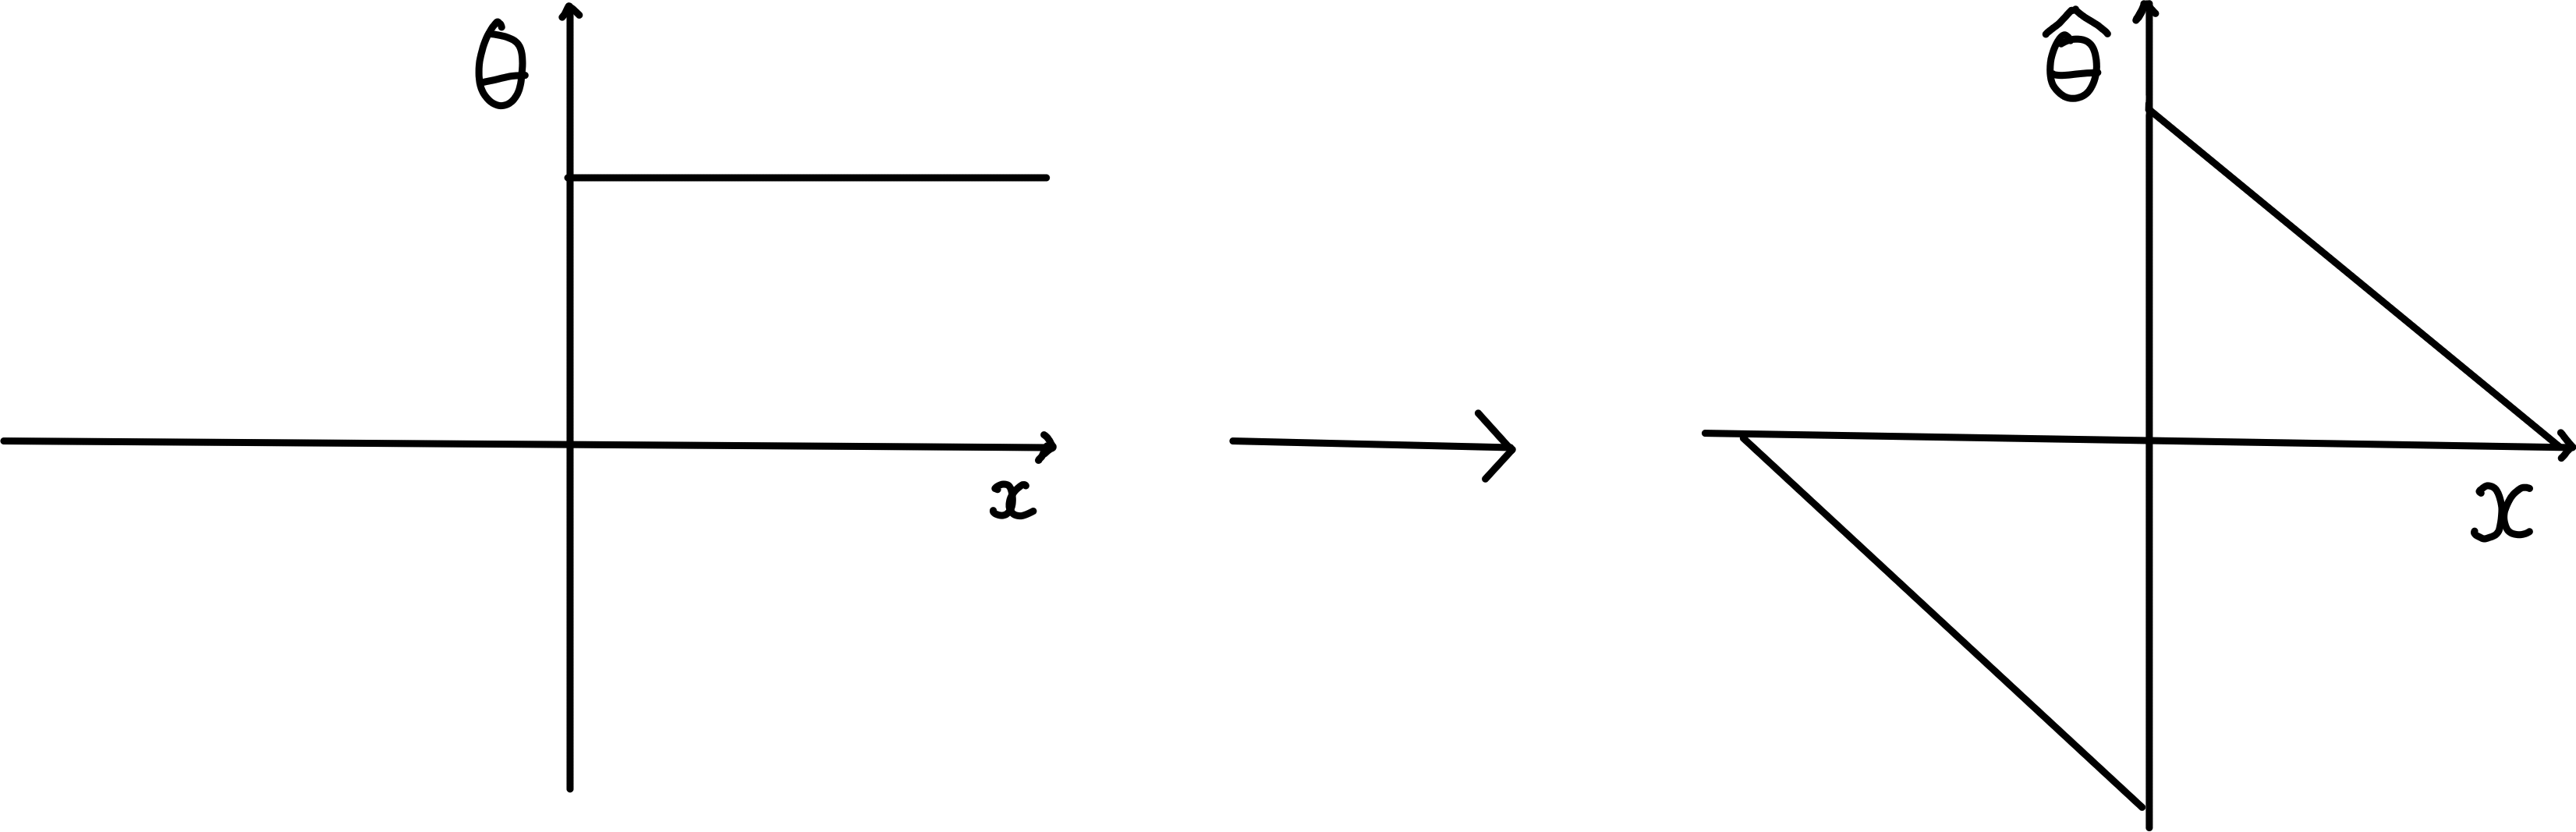
\includegraphics[height=5cm]{04-transformbcs} 
\end{figure}

\subsubsection{Seperation of variables}
We will now separate variables in the usual way.
We will consider the ansatz
\begin{align} \label{eq:4.12}
	\hat \theta(x,t) = X(x) T(t) \implies X'' = - \lambda X; \dot T = -D \lambda T
\end{align}
The boundary conditions imply $\lambda > 0$ and give the Fourier modes $X(x) = A \cos \sqrt{\lambda} x + B \sin \sqrt{\lambda} x$.
For $\cos \sqrt{\lambda} L = 0$, we require $\sqrt{\lambda_m} = \frac{m \pi}{2L}$ for $m$ odd.
Also, $\sin \sqrt{\lambda} L = 0$ gives $\sqrt{\lambda_n} = \frac{n \pi}{L}$ for $n$ even.
Since $\hat \theta$ is odd due to our initial conditions, we can take
\begin{align*}
	X_n = B_n \sin \frac{n \pi x}{L}; \quad \lambda_n = \frac{n^2 \pi^2}{L^2}
\end{align*}
Substituting $\lambda_n$ into \cref{eq:4.12}, $\dot T = -D \lambda T$, we have
\begin{align*}
	T_n(t) = C_n \exp(-\frac{Dn^2 \pi^2}{L^2} t ).
\end{align*}
In general, the solution is
\begin{align*}
	\hat \theta(x,t) = \sum_{n=1}^\infty b_n \sin \frac{n \pi x}{L} \exp(-\frac{Dn^2 \pi^2}{L^2} t )
\end{align*}

\subsection{Particular solution to diffusion equation}
Recall that
\begin{align*}
	\hat \theta(x,t) = \sum_{n=1}^\infty b_n \sin \frac{n \pi x}{L} \exp(-\frac{Dn^2 \pi^2}{L^2} t )
\end{align*}
At $t = 0$, we have a pure Fourier sine series.
We can then impose the initial conditions, to give
\begin{align*}
	b_n = \frac{1}{L} \int_{-L}^L \hat \phi(x,0) \sin \frac{n \pi x}{L} \dd{x}
\end{align*}
where
\begin{align*}
	\hat\phi(x,0) = H(x) - \frac{x+L}{2L}
\end{align*}
Hence, we can use the half-range sine series and find
\begin{align*}
	b_n = \underbrace{ \frac{2}{L} \int_0^L \qty(H(x) = \frac{1}{2}) \sin \frac{n \pi x}{L} \dd{x} }_{\text{square wave}/2} - \underbrace{ \frac{2}{L}\frac{x}{2L} \sin \frac{n \pi x}{L} \dd{x} }_{\text{sawtooth}/2L}
\end{align*}
which gives
\begin{align*}
	b_n = \frac{2}{(2m-1)\pi} - \frac{(-1)^{n+1}}{n\pi}
\end{align*}
where $n = 2m - 1$, and the first term vanishes for $n$ even.
For $n$ odd or even, we find the same result
\begin{align*}
	b_n = \frac{1}{n\pi}
\end{align*}
Hence
\begin{align*}
	\hat\theta(x,t) = \sum_{n=1}^\infty \frac{1}{n \pi} \sin \frac{n \pi x}{L} e^{-D \frac{n^2 \pi^2}{L^2} t}
\end{align*}
For the inhomogeneous boundary conditions,
\begin{align*}
	\theta(x,t) = \frac{x+L}{2L} + \sum_{n=1}^\infty \frac{1}{n \pi} \sin \frac{n \pi x}{L} e^{-D \frac{n^2 \pi^2}{L^2} t}
\end{align*}
The similarity solution $\frac{1}{2}\qty(1 + \erf(\frac{x}{2\sqrt{Dt}}))$ is a good fit for early $t$, but it does not necessarily satisfy the boundary conditions, so for large $t$ it is a bad approximation.

\subsection{Laplace's equation}
Laplace's equation is
\begin{align*}
	\laplacian \phi = 0
\end{align*}
This equation describes (among others) steady-state heat flow, potential theory $F = -\grad{\phi}$, and incompressible fluid flow $v = \grad{\phi}$.
The equation is solved typically on a domain $D$, where boundary conditions are specified often on the boundary surface.
The Dirichlet boundary conditions fix $\phi$ on the boundary surface $\partial D$.
The Neumann boundary conditions fix $\hat n \cdot \grad{\phi}$ on $\partial D$.

\subsection{Laplace's equation in three-dimensional Cartesian coordinates}
In $\mathbb R^3$ with Cartesian coordinates, Laplace's equation becomes
\begin{align*}
	\pdv[2]{\phi}{x} + \pdv[2]{\phi}{y} + \pdv[2]{\phi}{z} = 0
\end{align*}
We seek separable solutions in the usual way:
\begin{align*}
	\phi(x,y,z) = X(x)Y(y)Z(z)
\end{align*}
Substituting,
\begin{align*}
	X''YZ + XY''Z + XYZ'' = 0
\end{align*}
Dividing by $XYZ$ as usual,
\begin{align*}
	\frac{X''}{X} = \frac{-Y''}{Y} - \frac{Z''}{Z} & = -\lambda_\ell                         \\
	\frac{Y''}{Y} = \frac{-Z''}{Z} - \frac{X''}{X} & = -\lambda_m                            \\
	\frac{Z''}{Z} = \frac{-X''}{X} - \frac{Y''}{Y} & = -\lambda_n = \lambda_\ell + \lambda_m
\end{align*}
From the eigenmodes, our general solution will be of the form
\begin{align*}
	\phi(x,y,z) = \sum_{\ell,m,n} a_{\ell mn} X_\ell(x) Y_m(y) Z_n(z)
\end{align*}
Consider steady ($\pdv{\phi}{t} = 0$) heat flow in a semi-infinite rectangular bar, with boundary conditions $\phi = 0$ at $x = 0$, $x = a$, $y = 0$ and $y = b$; and $\phi = 1$ at $z = 0$ and $\phi \to 0$ as $z \to \infty$.
We will solve for each eigenmode successively.
First, consider $X'' = -\lambda_\ell X$ with $X(0) = X(a) = 0$.
This gives
\begin{align*}
	\lambda_\ell = \frac{l^2 \pi^2}{a^2};\quad X_\ell = \sin \frac{\ell \pi x}{a}
\end{align*}
where $\ell > 0, \ell \in \mathbb N$.
By symmetry,
\begin{align*}
	\lambda_m = \frac{m^2 \pi^2}{b^2};\quad Y_m = \sin \frac{m \pi y}{b}
\end{align*}
For the $z$ mode,
\begin{align*}
	Z'' = -\lambda_n Z = (\lambda_\ell + \lambda_m) Z = \pi^2\qty(\frac{\ell^2}{a^2} + \frac{m^2}{b^2}) Z
\end{align*}
Since $\phi \to 0$ as $z \to \infty$, the growing exponentials must vanish.
Therefore,
\begin{align*}
	Z_{\ell m} = \exp[-\qty(\frac{\ell^2}{a^2} + \frac{m^2}{b^2})^{1/2} \pi z]
\end{align*}
Thus the general solution is
\begin{align*}
	\phi(x,y,z) = \sum_{\ell, m} a_{\ell m} \sin \frac{\ell \pi x}{a} \sin \frac{m \pi y}{b} \exp[-\qty(\frac{\ell^2}{a^2} + \frac{m^2}{b^2})^{1/2} \pi z]
\end{align*}
Now, we will fix $a_{\ell m}$ using $\phi(x,y,0) = 1$ using the Fourier sine series.
\begin{align*}
	a_{\ell m} = \frac{2}{b} \int_0^b \frac{2}{a} \int_0^a \underbrace{1 \sin \frac{\ell \pi x}{a}}_{\text{square wave}} \underbrace{\sin \frac{m \pi y}{b}}_{\text{square wave}} \dd{x} \dd{y}
\end{align*}
So only the odd terms remain, giving
\begin{align*}
	a_{\ell m} = \frac{4a}{a(2k-1)\pi} \cdot \frac{4b}{b(2p-1) \pi}
\end{align*}
where $\ell = 2k-1$ is odd and $m = 2p-1$ is odd.
Simplifying,
\begin{align*}
	a_{\ell m} = \frac{16}{\pi^2 \ell m} \quad \text{ for } \ell, m \text{ odd}
\end{align*}
So the heat flow solution is
\begin{align*}
	\phi(x,y,z) = \sum_{\ell, m \text{ odd}} \frac{16}{\pi^2 \ell m} \sin \frac{\ell \pi x}{a} \sin \frac{\ell \pi y}{b} \exp[-\qty(\frac{\ell^2}{a^2} + \frac{m^2}{b^2})^{1/2} \pi z]
\end{align*}
As $z$ increases, every contribution but the lowest mode will be very small.
So low $\ell, m$ dominate the solution.

\subsection{Laplace's equation in plane polar coordinates}
In plane polar coordinates, Laplace's equation becomes
\begin{align*}
	\frac{1}{r} \pdv{r} \qty(r \pdv{\phi}{r}) + \frac{1}{r^2} \pdv[2]{\phi}{\theta} = 0
\end{align*}
Consider a separable form of the answer, given by
\begin{align*}
	\phi(r,\theta) = R(r) \Theta(\theta)
\end{align*}
We then have
\begin{align*}
	\Theta'' + \mu \Theta = 0;\quad r(rR')' - \mu R = 0
\end{align*}
The polar equation can be solved easily by considering periodic boundary conditions.
This gives $\mu = m^2$ and the eigenmodes
\begin{align*}
	\Theta_m(\theta) = \cos m \theta, \sin m \theta
\end{align*}
The radial equation is \textit{not} Bessel's equation, since there is no second separation constant.
We simply have
\begin{align*}
	r(rR')' - m^2 R = 0
\end{align*}
We will try a power law solution, $r = \alpha r^\beta$.
We find
\begin{align*}
	\beta^2 - m^2 = 0 \implies \beta = \pm m
\end{align*}
So the eigenfunctions are
\begin{align*}
	R_m(r) = r^m, r^{-m}
\end{align*}
which is one regular solution at the origin and one singular solution.
In the case $m = 0$, we have
\begin{align*}
	(rR') = 0 \implies rR' = \text{constant} \implies R = \log r
\end{align*}
So
\begin{align*}
	R_0(r) = \text{constant}, \log r
\end{align*}
The general solution is therefore
\begin{align*}
	\phi(r,\theta) = \frac{a_0}{2} + c_0 \log r + \sum_{m=1}^\infty \qty(a_m \cos m\theta + b_m \sin m\theta) r^m + \sum_{m=1}^\infty \qty(c_m \cos m\theta + d_m \sin m\theta) r^{-m}
\end{align*}
\begin{example}
	Consider a soap film on a unit disc.
	We wish to solve Laplace's equation with a vertically distorted circular wire of radius $r = 1$ with boundary conditions $\phi(1, \theta) = f(\theta)$.
	The $z$ displacement of the wire produces the $f(\theta)$ term.
	We wish to find $\phi(r,\theta)$ for $r < 1$, assuming regularity at $r = 0$.
	Then, $c_m = d_m = 0$ and the solution is of the form
	\begin{align*}
		\phi(r,\theta) = \frac{a_0}{2} + \sum_{m=1}^\infty \qty(a_m \cos m\theta + b_m \sin m\theta) r^m
	\end{align*}
	At $r = 1$,
	\begin{align*}
		\phi(1,\theta) = f(\theta) = \frac{a_0}{2} + \sum_{m=1}^\infty \qty(a_m \cos m\theta + b_m \sin m\theta)
	\end{align*}
	which is exactly the Fourier series.
	Thus,
	\begin{align*}
		a_m = \frac{1}{\pi} \int_0^{2\pi} f(\theta) \cos m \theta \dd{\theta};\quad b_m = \frac{1}{\pi} \int_0^{2\pi} f(\theta) \sin m \theta \dd{\theta}
	\end{align*}
	We can see from the equation that high harmonics are confined to have effects only near $r = 1$.
\end{example}

\subsection{Laplace's equation in cylindrical polar coordinates}
In cylindrical coordinates,
\begin{align*}
	\frac{1}{r} \pdv{r} \qty(r \pdv{\phi}{r}) + \frac{1}{4^2} \pdv[2]{\phi}{\theta} + \pdv[2]{\phi}{z} = 0
\end{align*}
With $\phi = R(r) \Theta(\theta) Z(z)$, we find
\begin{align*}
	\Theta'' = -\mu \Theta;\quad Z'' = \lambda Z;\quad r(rR')' + (\lambda r^2 - \mu) R = 0
\end{align*}
The polar equation can be easily solved by
\begin{align*}
	\mu_m = m^2;\quad \Theta_m(\theta) = \cos m\theta, \sin m\theta
\end{align*}
The radial equation is Bessel's equation, giving solutions
\begin{align*}
	R = J_m(kr), Y_m(kr)
\end{align*}
Setting boundary conditions in the usual way, defining $R=0$ at $r = a$ means that
\begin{align*}
	J_m(ka) = 0 \implies k = \frac{j_{mn}}{a}
\end{align*}
The radial solution is
\begin{align*}
	R_{mn}(r) = J_m\qty(\frac{j_{mn}}{a}r)
\end{align*}
We have eliminated the $Y_n$ term since we require $r = 0$ to give a finite $\phi$.
Finally, the $z$ equation gives
\begin{align*}
	Z'' = k^2 Z \implies Z = e^{-kz}, e^{kz}
\end{align*}
We typically eliminate the $e^{kz}$ mode due to boundary conditions, such as $Z \to 0$ as $z \to \infty$.
The general solution is therefore
\begin{align*}
	\phi(r,\theta,z) = \sum_{m=0}^\infty \sum_{n = 1}^\infty \qty(a_{mn} \cos m\theta + b_{mn} \sin m\theta) J_m\qty(\frac{j_{mn}}{a} r) e^{-frac{j_{mn}r}{a}}
\end{align*}

\subsection{Laplace's equation in spherical polar coordinates}
In spherical polar coordinates,
\begin{align*}
	\frac{1}{r^2} \pdv{r} \qty(r^2 \pdv{\Phi}{r}) + \frac{1}{r^2 \sin\theta}\pdv{\theta} \qty(\sin\theta \pdv{\Phi}{\theta}) + \frac{1}{r^2 \sin^2 \theta} \pdv[2]{\Phi}{\phi} = 0
\end{align*}
We will consider the \textit{axisymmetric case}; supposing that there is no $\phi$ dependence.
We seek a separable solution of the form
\begin{align*}
	\Phi(r,\theta) = R(r) \Theta(\theta)
\end{align*}
which gives
\begin{align*}
	(\sin\theta \Theta')' + \lambda \sin\theta \Theta = 0;\quad (r^2R')' - \lambda R = 0
\end{align*}
Consider the substitution $x = \cos\theta, \dv{x}{\theta} = -\sin\theta$ in the polar equation.
This gives $\dv{\Theta}{\theta} = -\sin\theta \dv{\Theta}{x}$ and hence
\begin{align*}
	-\sin\theta \dv{x}\qty[-\sin^2\theta \dv{\Theta}{x}] + \lambda \sin\theta \Theta = 0 \implies \dv{x}\qty[(1-x^2)\dv{\Theta}{x}] + \lambda \Theta = 0
\end{align*}
This gives Legendre's equation, so it has solutions of eigenvalues $\lambda_\ell = \ell (\ell + 1)$ and eigenfunctions
\begin{align*}
	\Theta_\ell(\theta) = P_\ell(x) = P_\ell(\cos\theta)
\end{align*}
The radial equation then gives
\begin{align*}
	(r^2 R')' - \ell (\ell + 1) R = 0
\end{align*}
We will seek power law solutions: $R = \alpha r^\beta$.
This gives
\begin{align*}
	\beta(\beta + 1) - \ell(\ell + 1) = 0 \implies \beta = \ell, \beta = -\ell - 1
\end{align*}
Thus the radial eigenmodes are
\begin{align*}
	R_\ell = r^{\ell}, r^{-\ell - 1}
\end{align*}
Therefore the general axisymmetric solution for spherical polar coordinates is
\begin{align*}
	\Phi(r,\theta) = \sum_{\ell = 0}^\infty (a_\ell r^{\ell} + b_\ell r^{-\ell - 1}) P_\ell(\cos\theta)
\end{align*}
The $a_\ell, b_\ell$ are determined by the boundary conditions.
Orthogonality conditions for the $P_\ell$ can be used to determine coefficients.
Consider a solution to Laplace's equation on the unit sphere with axisymmetric boundary conditions given by
\begin{align*}
	\Phi(1,\theta) = f(\theta)
\end{align*}
Given that we wish to find the interior solution, $b_n = 0$ by regularity.
Then,
\begin{align*}
	f(\theta) = \sum_{\ell=0}^\infty a_\ell P_\ell(\cos\theta)
\end{align*}
By defining $f(\theta) = F(\cos\theta)$,
\begin{align*}
	F(x) = \sum_{\ell=0}^\infty a_\ell P_\ell(x)
\end{align*}
We can then find the coefficients in the usual way, giving
\begin{align*}
	a_\ell = \frac{2\ell + 1}{2} \int_{-1}^1 F(x) P_{\ell}(x) \dd{x}
\end{align*}

\subsection{Generating function for Legendre polynomials}
Consider a charge at $r_0 = (x,y,z) = (0,0,1)$.
Then, the potential at a point $P$ becomes
\begin{align*}
	\Phi(r) & = \frac{1}{\abs{r - r_0}} = \frac{1}{(x^2 + y^2 + (x-1)^2)^{1/2}} \\
	& = \frac{1}{(r^2 (\sin^2 \phi + \cos^2 \phi) \sin^2 \theta + r^2 \cos^2 \theta - 2r \cos\theta + 1)^{1/2}} \\
	& = \frac{1}{(r^2 \sin^2 \theta + r^2 \cos^2 \theta - 2r \cos\theta + 1)^{1/2}} \\
	& = \frac{1}{(r^2 - 2r \cos\theta + 1)^{1/2}} \\
	& = \frac{1}{(r^2 - 2r \overline x + 1)^{1/2}}
\end{align*}
where 

$\overline x \equiv \cos \theta$.
This function $\Phi$ is a solution to Laplace's equation where $r \neq r_0$.
Note that we can represent any axisymmetric solution as a sum of Legendre polynomials.
Now,
\begin{align*}
	\frac{1}{\sqrt{r^2 - 2rx + 1}} = \sum_{\ell = 0}^\infty a_\ell P_\ell(x) r^\ell
\end{align*}
With the normalisation condition for the Legendre polynomials $P_\ell(1) = 1$, we find
\begin{align*}
	\frac{1}{1-r} = \sum_{\ell=0}^\infty a_\ell r^\ell
\end{align*}
Using the geometric series expansion, we arrive at $a_\ell = 1$.
This gives
\begin{align*}
	\frac{1}{\sqrt{r^2 - 2rx + 1}} = \sum_{\ell = 0}^\infty P_\ell(x) r^\ell
\end{align*}
which is the generating function for the Legendre polynomials.
    \section{The Laplace Equation}

\subsection{Laplace's equation}
Laplace's equation is
\begin{align} \label{eq:5.1}
	\laplacian \phi = 0
\end{align}
This equation describes (among others) steady-state heat flow, potential theory $F = -\grad{\phi}$, and incompressible fluid flow $v = \grad{\phi}$.
The equation \cref{eq:5.1} is solved typically on a domain $D$, where boundary conditions are specified often on the boundary surface.
The Dirichlet boundary conditions fix $\phi$ on the boundary surface $\partial D$.
The Neumann boundary conditions fix $\hat n \cdot \grad{\phi}$ on $\partial D$.

\subsection{Laplace's equation in three-dimensional Cartesian coordinates}
In $\mathbb R^3$ with Cartesian coordinates, Laplace's equation becomes
\begin{align} \label{eq:5.2}
	\pdv[2]{\phi}{x} + \pdv[2]{\phi}{y} + \pdv[2]{\phi}{z} = 0
\end{align}
We seek separable solutions in the usual way:
\begin{align*}
	\phi(x,y,z) = X(x)Y(y)Z(z)
\end{align*}
Substituting,
\begin{align*}
	X''YZ + XY''Z + XYZ'' = 0
\end{align*}
Dividing by $XYZ$ as usual,
\begin{align*}
	\frac{X''}{X} = \frac{-Y''}{Y} - \frac{Z''}{Z} & = -\lambda_\ell \quad \text{(constant)}\\
	\frac{Y''}{Y} = \frac{-Z''}{Z} - \frac{X''}{X} & = -\lambda_m \quad \text{(constant)} \\
	\frac{Z''}{Z} = \frac{-X''}{X} - \frac{Y''}{Y} & = -\lambda_n = \lambda_\ell + \lambda_m
\end{align*}
From the eigenmodes, our general solution will be of the form
\addtocounter{equation}{1}
\begin{align} \label{eq:5.4}
	\phi(x,y,z) = \sum_{\ell,m,n} a_{\ell mn} X_\ell(x) Y_m(y) Z_n(z)
\end{align}

\begin{example}[Steady heat conduction]
    Consider steady ($\pdv{\phi}{t} = 0$) heat flow\footnote{i.e. \cref{eq:4.3} with $\pdv{\phi}{t} = 0$ gives \cref{eq:5.1}} in a semi-infinite rectangular bar, with boundary conditions $\phi = 0$ at $x = 0$, $x = a$, $y = 0$ and $y = b$; and $\phi = 1$ at $z = 0$ and $\phi \to 0$ as $z \to \infty$.
    {\par
    \centering 
    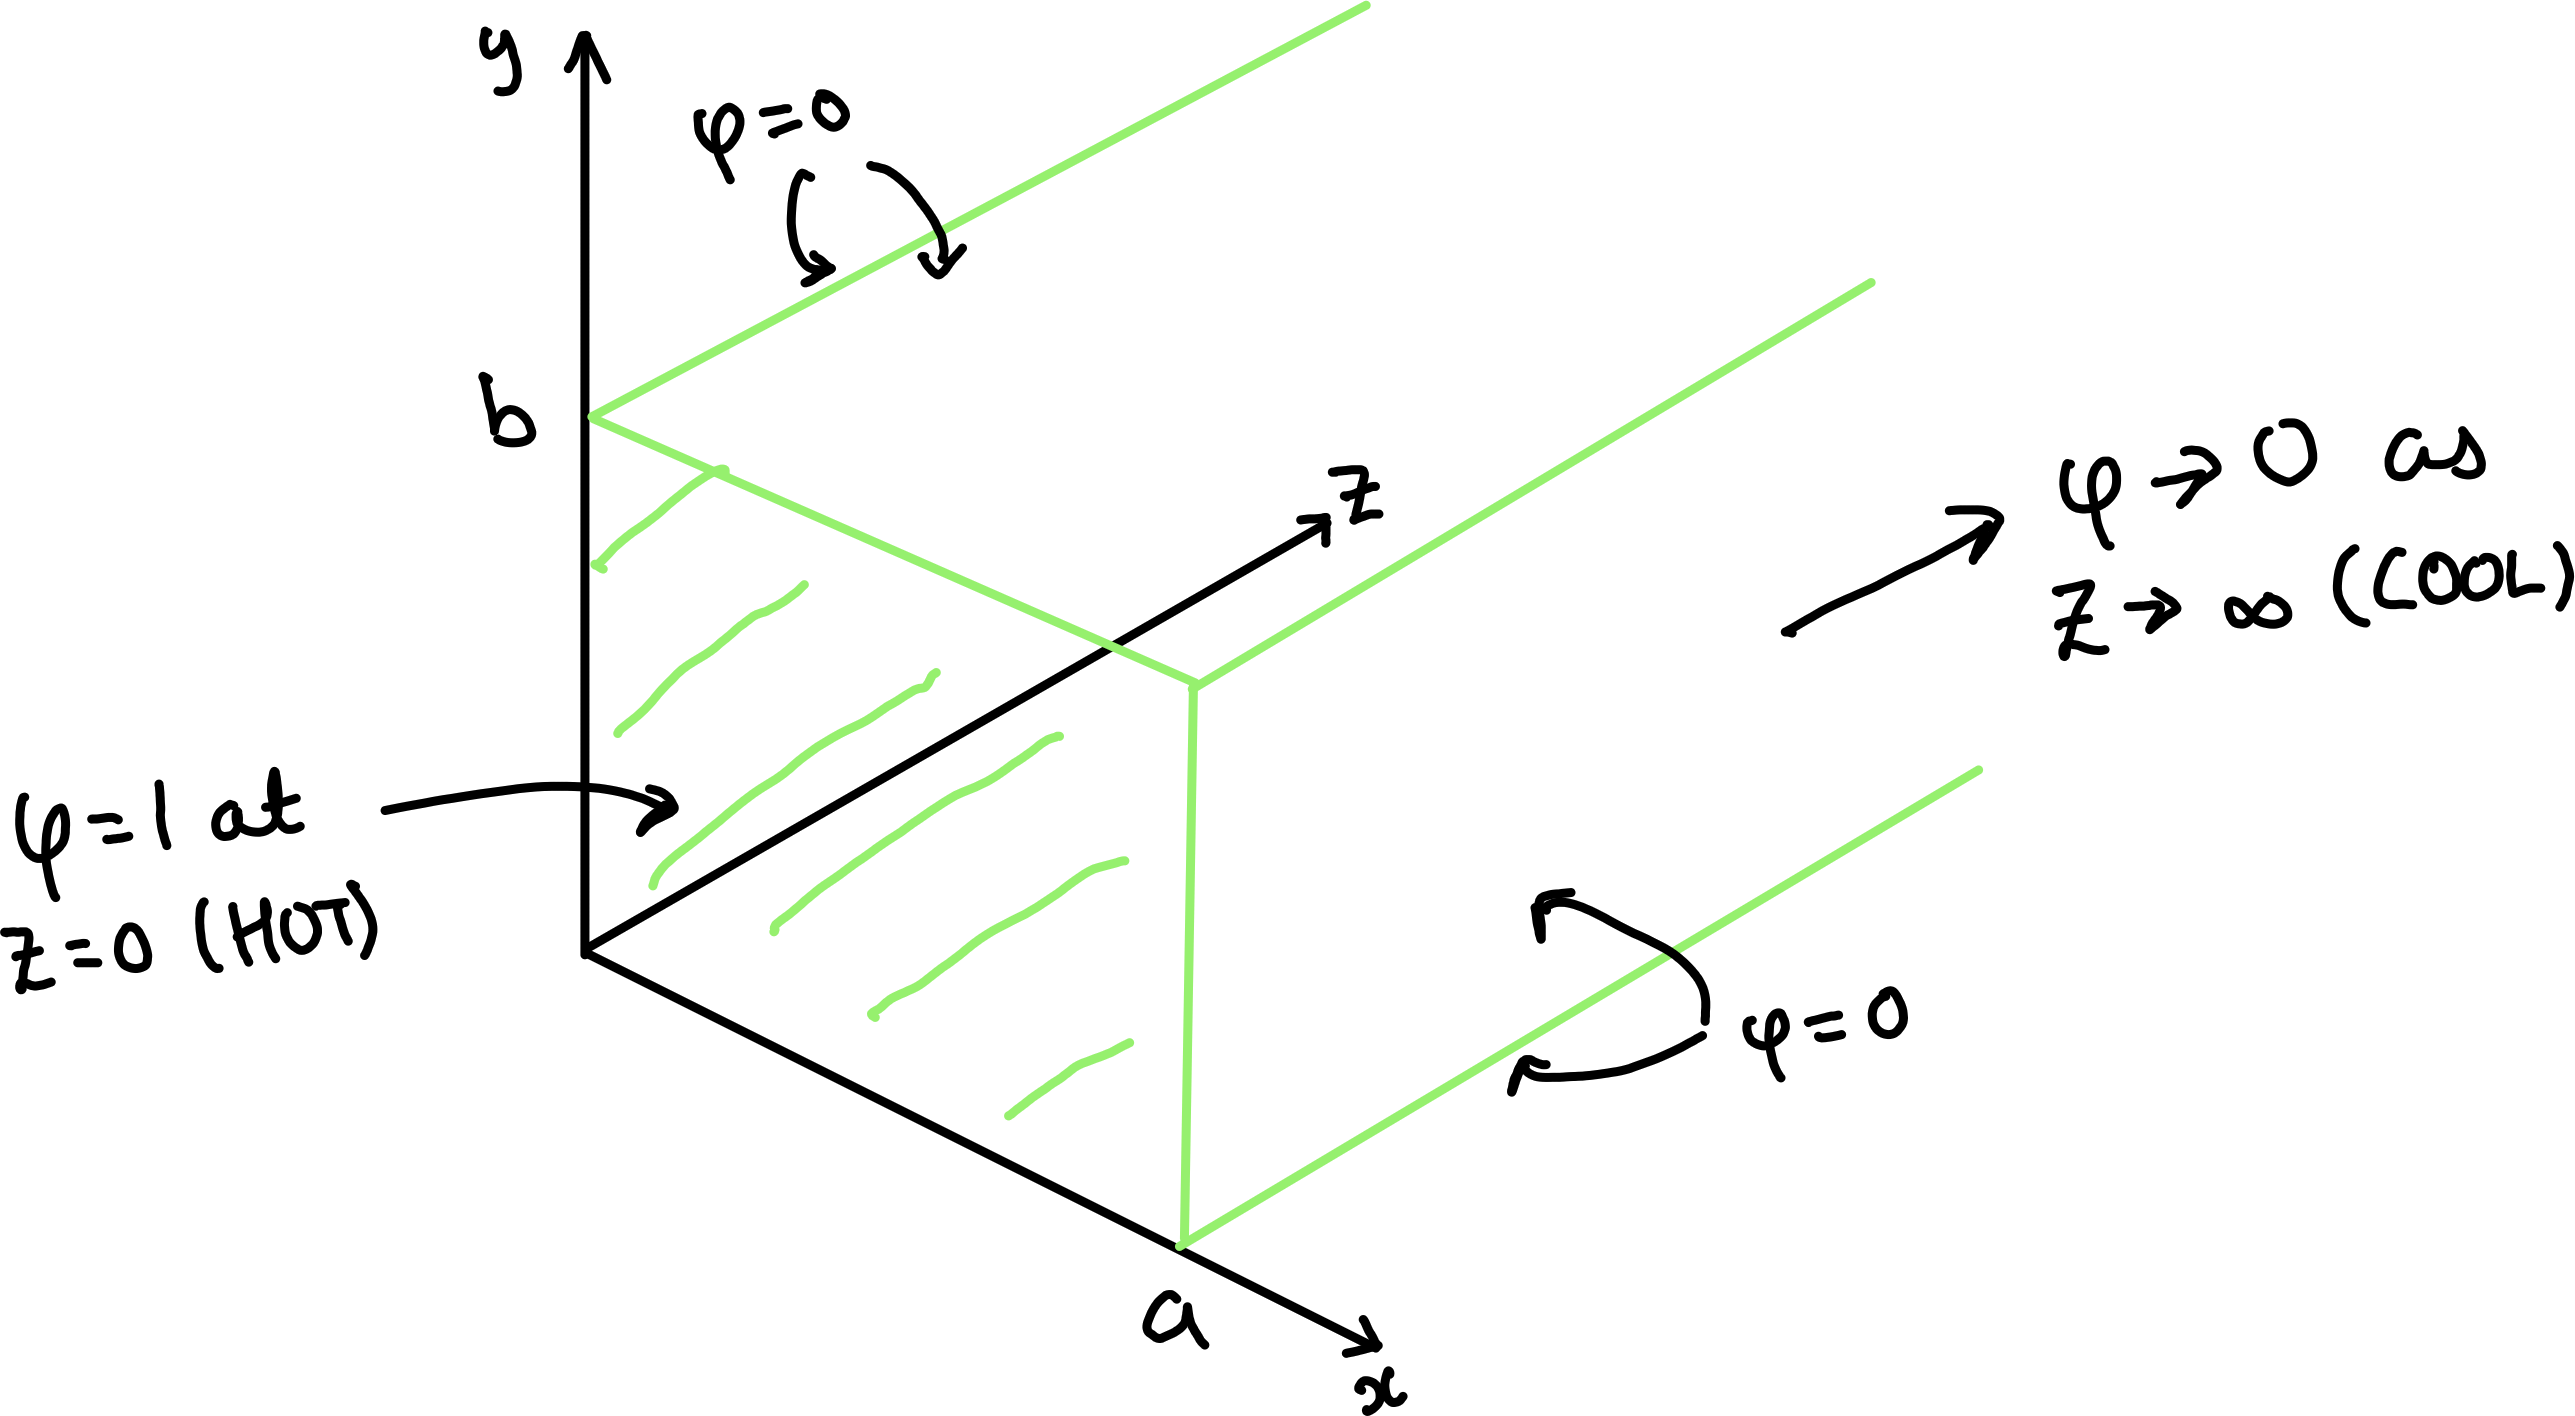
\includegraphics[height=5cm]{05-exm-steadyheat} 
    \par}
    We will solve for each eigenmode successively.
    First, consider $X'' = -\lambda_\ell X$ with $X(0) = X(a) = 0$.
    This gives
    \begin{align*}
        \lambda_\ell = \frac{l^2 \pi^2}{a^2};\quad X_\ell = \sin \frac{\ell \pi x}{a}
    \end{align*}
    where $\ell > 0, \ell \in \mathbb N$.
    By symmetry,
    \begin{align*}
        \lambda_m = \frac{m^2 \pi^2}{b^2};\quad Y_m = \sin \frac{m \pi y}{b}
    \end{align*}
    For the $z$ mode,
    \begin{align*}
        Z'' = -\lambda_n Z = (\lambda_\ell + \lambda_m) Z = \pi^2\qty(\frac{\ell^2}{a^2} + \frac{m^2}{b^2}) Z
    \end{align*}
    Since $\phi \to 0$ as $z \to \infty$, the growing exponentials must vanish.
    Therefore,
    \begin{align*}
        Z_{\ell m} = \exp[-\qty(\frac{\ell^2}{a^2} + \frac{m^2}{b^2})^{1/2} \pi z]
    \end{align*}
    Thus the general solution \cref{eq:5.4} becomes
    \begin{align*}
        \phi(x,y,z) = \sum_{\ell, m} a_{\ell m} \sin \frac{\ell \pi x}{a} \sin \frac{m \pi y}{b} \exp[-\qty(\frac{\ell^2}{a^2} + \frac{m^2}{b^2})^{1/2} \pi z]
    \end{align*}
    Now, we will fix $a_{\ell m}$ using $\phi(x,y,0) = 1$ using the Fourier sine series \cref{eq:1.12}.
    \begin{align*}
        a_{\ell m} = \frac{2}{b} \int_0^b \frac{2}{a} \int_0^a \underbrace{1 \sin \frac{\ell \pi x}{a}}_{\text{square wave}} \underbrace{\sin \frac{m \pi y}{b}}_{\text{square wave}} \dd{x} \dd{y}
    \end{align*}
    So only the odd terms remain, giving
    \begin{align*}
        a_{\ell m} = \frac{4a}{a(2k-1)\pi} \cdot \frac{4b}{b(2p-1) \pi}
    \end{align*}
    where $\ell = 2k-1$ is odd and $m = 2p-1$ is odd.
    Simplifying,
    \begin{align*}
        a_{\ell m} = \frac{16}{\pi^2 \ell m} \quad \text{ for } \ell, m \text{ odd}
    \end{align*}
    So the heat flow solution is
    \begin{align*}
        \phi(x,y,z) = \sum_{\ell, m \text{ odd}} \frac{16}{\pi^2 \ell m} \sin \frac{\ell \pi x}{a} \sin \frac{\ell \pi y}{b} \exp[-\qty(\frac{\ell^2}{a^2} + \frac{m^2}{b^2})^{1/2} \pi z]
    \end{align*}
    As $z$ increases, every contribution but the lowest mode will be very small.
    So low $\ell, m$ dominate the solution.

    Cross sectionals:
    insertpicture
\end{example} 

\subsection{Laplace's equation in plane polar coordinates}
In plane polar coordinates, Laplace's equation becomes
\addtocounter{equation}{1}
\begin{align} \label{eq:5.6}
	\frac{1}{r} \pdv{r} \qty(r \pdv{\phi}{r}) + \frac{1}{r^2} \pdv[2]{\phi}{\theta} = 0
\end{align}
Consider a separable form of the answer, given by
\begin{align*}
	\phi(r,\theta) = R(r) \Theta(\theta)
\end{align*}
We then have
\begin{align*}
	\Theta'' + \mu \Theta = 0;\quad r(rR')' - \mu R = 0
\end{align*}

\subsubsection{Polar equation}
The polar equation can be solved easily by considering periodic boundary conditions.
This gives $\mu = m^2$ and the eigenmodes as in \cref{eq:3.25}
\begin{align*}
	\Theta_m(\theta) = \cos m \theta, \sin m \theta
\end{align*}

\subsubsection{Radial equation}
The radial equation is \textit{not} Bessel's equation, since there is no second separation constant.
We simply have
\begin{align} \label{eq:5.7}
	r(rR')' - m^2 R = 0
\end{align}
We will try a power law solution, $R = \alpha r^\beta$.
We find
\begin{align*}
	\beta^2 - m^2 = 0 \implies \beta = \pm m
\end{align*}
So the eigenfunctions are
\begin{align*}
	R_m(r) = r^m, r^{-m}
\end{align*}
which is one regular solution at the origin and one singular solution. \\
In the case $m = 0$, we have
\begin{align*}
	(rR')' = 0 \implies rR' = \text{constant} \implies R = \log r
\end{align*}
So
\begin{align*}
	R_0(r) = \text{constant or } \log r
\end{align*}
The general solution is therefore
\begin{align} \label{eq:5.8}
	\phi(r,\theta) = \frac{a_0}{2} + c_0 \log r + \sum_{m=1}^\infty \qty(a_m \cos m\theta + b_m \sin m\theta) r^m + \sum_{m=1}^\infty \qty(c_m \cos m\theta + d_m \sin m\theta) r^{-m}
\end{align}

\begin{example}[Soap Film on a Unit Disc]
    insertpicture

	Consider a soap film on a unit disc.
	We wish to solve Laplace's equation \cref{eq:5.6} with a vertically distorted circular wire of radius $r = 1$ with boundary conditions $\phi(1, \theta) = f(\theta)$.
	The $z$ displacement of the wire produces the $f(\theta)$ term.
	We wish to find $\phi(r,\theta)$ for $r < 1$, assuming regularity at $r = 0$.
	Then, $c_m = d_m = 0$ and so \cref{eq:5.8} becomes
	\begin{align*}
		\phi(r,\theta) = \frac{a_0}{2} + \sum_{m=1}^\infty \qty(a_m \cos m\theta + b_m \sin m\theta) r^m
	\end{align*}
	At $r = 1$,
	\begin{align*}
		\phi(1,\theta) = f(\theta) = \frac{a_0}{2} + \sum_{m=1}^\infty \qty(a_m \cos m\theta + b_m \sin m\theta)
	\end{align*}
	which is exactly the Fourier series.
	Thus by \cref{eq:1.5},
	\begin{align*}
		a_m = \frac{1}{\pi} \int_0^{2\pi} f(\theta) \cos m \theta \dd{\theta};\quad b_m = \frac{1}{\pi} \int_0^{2\pi} f(\theta) \sin m \theta \dd{\theta}
	\end{align*}
	We can see from the equation that high harmonics are confined to have effects only near $r = 1$.
\end{example}

\begin{figure}[h] 
    \centering 
    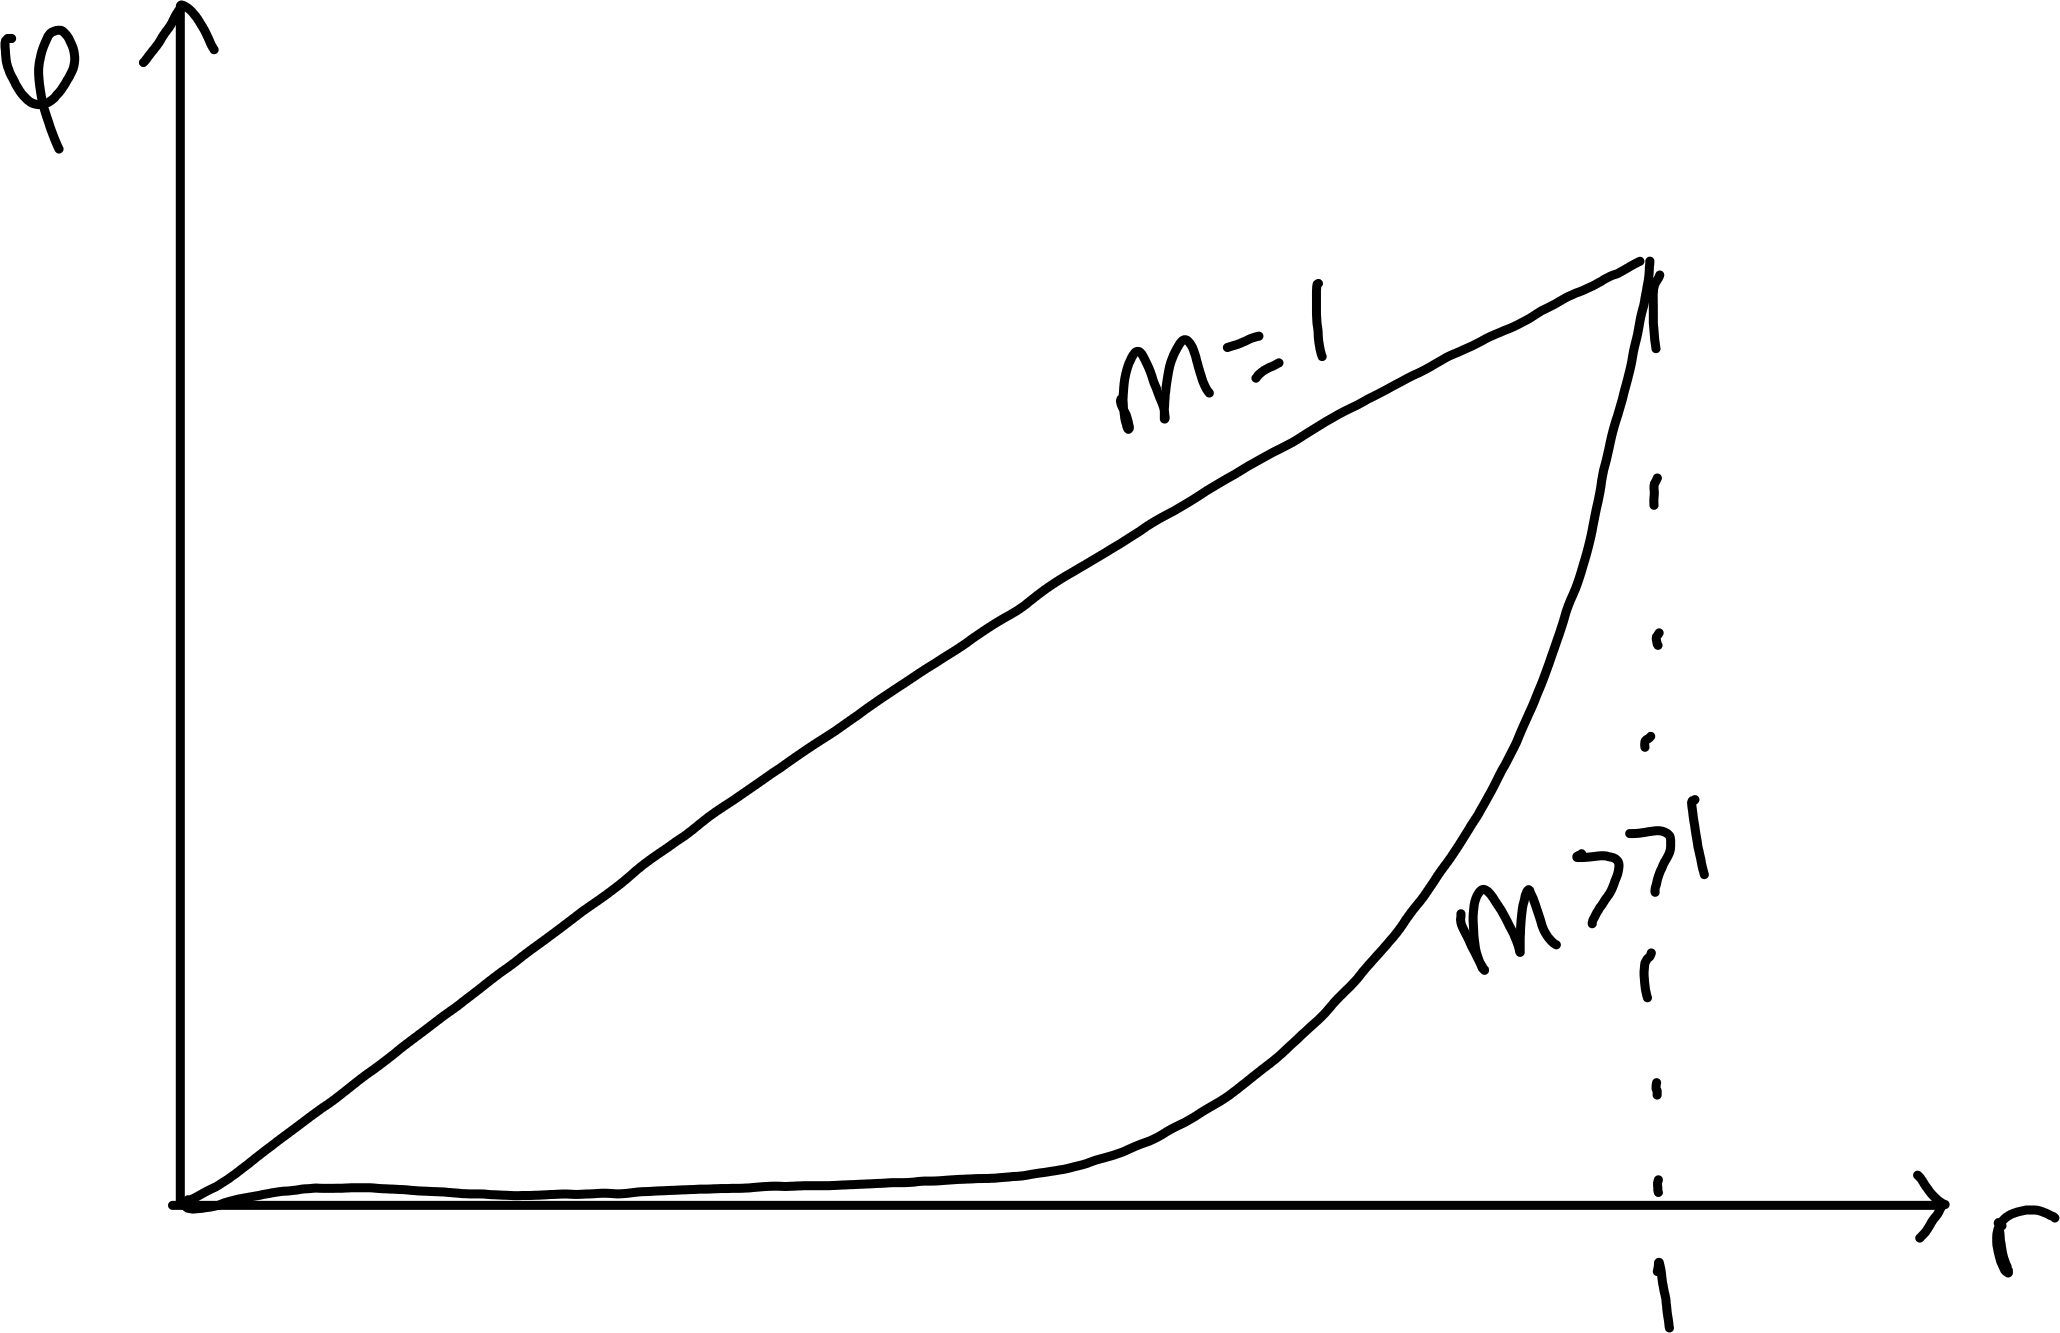
\includegraphics[height=5cm]{05-polarsoln} 
\end{figure}

\subsection{Laplace's equation in cylindrical polar coordinates}
In cylindrical coordinates,
\begin{align*}
	\frac{1}{r} \pdv{r} \qty(r \pdv{\phi}{r}) + \frac{1}{4^2} \pdv[2]{\phi}{\theta} + \pdv[2]{\phi}{z} = 0
\end{align*}
With $\phi = R(r) \Theta(\theta) Z(z)$, we find
\begin{align*}
	\Theta'' = -\mu \Theta;\quad Z'' = \lambda Z;\quad r(rR')' + (\lambda r^2 - \mu) R = 0
\end{align*}
The polar equation can be easily solved by
\begin{align*}
	\mu_m = m^2;\quad \Theta_m(\theta) = \cos m\theta, \sin m\theta
\end{align*}
The radial equation is Bessel's equation, giving solutions
\begin{align*}
	R = J_m(kr), Y_m(kr)
\end{align*}
Setting boundary conditions in the usual way, defining $R=0$ at $r = a$ means that
\begin{align*}
	J_m(ka) = 0 \implies k = \frac{j_{mn}}{a}
\end{align*}
The radial solution is
\begin{align*}
	R_{mn}(r) = J_m\qty(\frac{j_{mn}}{a}r)
\end{align*}
We have eliminated the $Y_n$ term since we require $r = 0$ to give a finite $\phi$.
Finally, the $z$ equation gives
\begin{align*}
	Z'' = k^2 Z \implies Z = e^{-kz}, e^{kz}
\end{align*}
We typically eliminate the $e^{kz}$ mode due to boundary conditions, such as $Z \to 0$ as $z \to \infty$.
The general solution is therefore
\begin{align*}
	\phi(r,\theta,z) = \sum_{m=0}^\infty \sum_{n = 1}^\infty \qty(a_{mn} \cos m\theta + b_{mn} \sin m\theta) J_m\qty(\frac{j_{mn}}{a} r) e^{-frac{j_{mn}r}{a}}
\end{align*}

\subsection{Laplace's equation in spherical polar coordinates}
In spherical polar coordinates,
\begin{align*}
	\frac{1}{r^2} \pdv{r} \qty(r^2 \pdv{\Phi}{r}) + \frac{1}{r^2 \sin\theta}\pdv{\theta} \qty(\sin\theta \pdv{\Phi}{\theta}) + \frac{1}{r^2 \sin^2 \theta} \pdv[2]{\Phi}{\phi} = 0
\end{align*}
We will consider the \textit{axisymmetric case}; supposing that there is no $\phi$ dependence.
We seek a separable solution of the form
\begin{align*}
	\Phi(r,\theta) = R(r) \Theta(\theta)
\end{align*}
which gives
\begin{align*}
	(\sin\theta \Theta')' + \lambda \sin\theta \Theta = 0;\quad (r^2R')' - \lambda R = 0
\end{align*}
Consider the substitution $x = \cos\theta, \dv{x}{\theta} = -\sin\theta$ in the polar equation.
This gives $\dv{\Theta}{\theta} = -\sin\theta \dv{\Theta}{x}$ and hence
\begin{align*}
	-\sin\theta \dv{x}\qty[-\sin^2\theta \dv{\Theta}{x}] + \lambda \sin\theta \Theta = 0 \implies \dv{x}\qty[(1-x^2)\dv{\Theta}{x}] + \lambda \Theta = 0
\end{align*}
This gives Legendre's equation, so it has solutions of eigenvalues $\lambda_\ell = \ell (\ell + 1)$ and eigenfunctions
\begin{align*}
	\Theta_\ell(\theta) = P_\ell(x) = P_\ell(\cos\theta)
\end{align*}
The radial equation then gives
\begin{align*}
	(r^2 R')' - \ell (\ell + 1) R = 0
\end{align*}
We will seek power law solutions: $R = \alpha r^\beta$.
This gives
\begin{align*}
	\beta(\beta + 1) - \ell(\ell + 1) = 0 \implies \beta = \ell, \beta = -\ell - 1
\end{align*}
Thus the radial eigenmodes are
\begin{align*}
	R_\ell = r^{\ell}, r^{-\ell - 1}
\end{align*}
Therefore the general axisymmetric solution for spherical polar coordinates is
\begin{align*}
	\Phi(r,\theta) = \sum_{\ell = 0}^\infty (a_\ell r^{\ell} + b_\ell r^{-\ell - 1}) P_\ell(\cos\theta)
\end{align*}
The $a_\ell, b_\ell$ are determined by the boundary conditions.
Orthogonality conditions for the $P_\ell$ can be used to determine coefficients.
Consider a solution to Laplace's equation on the unit sphere with axisymmetric boundary conditions given by
\begin{align*}
	\Phi(1,\theta) = f(\theta)
\end{align*}
Given that we wish to find the interior solution, $b_n = 0$ by regularity.
Then,
\begin{align*}
	f(\theta) = \sum_{\ell=0}^\infty a_\ell P_\ell(\cos\theta)
\end{align*}
By defining $f(\theta) = F(\cos\theta)$,
\begin{align*}
	F(x) = \sum_{\ell=0}^\infty a_\ell P_\ell(x)
\end{align*}
We can then find the coefficients in the usual way, giving
\begin{align*}
	a_\ell = \frac{2\ell + 1}{2} \int_{-1}^1 F(x) P_{\ell}(x) \dd{x}
\end{align*}

\subsection{Generating function for Legendre polynomials}
Consider a charge at $r_0 = (x,y,z) = (0,0,1)$.
Then, the potential at a point $P$ becomes
\begin{align*}
	\Phi(r) & = \frac{1}{\abs{r - r_0}} = \frac{1}{(x^2 + y^2 + (x-1)^2)^{1/2}} \\
	& = \frac{1}{(r^2 (\sin^2 \phi + \cos^2 \phi) \sin^2 \theta + r^2 \cos^2 \theta - 2r \cos\theta + 1)^{1/2}} \\
	& = \frac{1}{(r^2 \sin^2 \theta + r^2 \cos^2 \theta - 2r \cos\theta + 1)^{1/2}} \\
	& = \frac{1}{(r^2 - 2r \cos\theta + 1)^{1/2}} \\
	& = \frac{1}{(r^2 - 2r \overline x + 1)^{1/2}}
\end{align*}
where 

$\overline x \equiv \cos \theta$.
This function $\Phi$ is a solution to Laplace's equation where $r \neq r_0$.
Note that we can represent any axisymmetric solution as a sum of Legendre polynomials.
Now,
\begin{align*}
	\frac{1}{\sqrt{r^2 - 2rx + 1}} = \sum_{\ell = 0}^\infty a_\ell P_\ell(x) r^\ell
\end{align*}
With the normalisation condition for the Legendre polynomials $P_\ell(1) = 1$, we find
\begin{align*}
	\frac{1}{1-r} = \sum_{\ell=0}^\infty a_\ell r^\ell
\end{align*}
Using the geometric series expansion, we arrive at $a_\ell = 1$.
This gives
\begin{align*}
	\frac{1}{\sqrt{r^2 - 2rx + 1}} = \sum_{\ell = 0}^\infty P_\ell(x) r^\ell
\end{align*}
which is the generating function for the Legendre polynomials.
    \section{Dirac delta function}

\begin{definition}[Dirac Delta Function]
	We define a generalised function $\delta(x - \xi)$ such that
	\begin{align}
		\begin{aligned} \label{eq:6.1}
			&\delta(x-\xi) = 0 \ \ \forall \; x \neq \xi; \\
			&\int_{-\infty}^\infty \delta(x-\xi) \dd{x} = 1.
		\end{aligned} 	
	\end{align} 
	% \begin{enumerate}
	% 	\item $\delta(x-\xi) = 0$ for all $x \neq \xi$;
	% 	\item $\int_{-\infty}^\infty \delta(x-\xi) \dd{x} = 1$.
	% \end{enumerate}
	This acts as a linear operator $\int \dd{x} \delta(x - \xi)$ on some arbitrary function $f(x)$ to produce a number $f(\xi)$.
	\begin{align} \label{eq:6.2}
		\int_{-\infty}^\infty \dd{x} \delta(x-\xi) f(x) = f(\xi)
	\end{align}
	This relationship holds provided that $f(x)$ is sufficiently `well-behaved' at $x=\xi$ and $x\to\pm \infty$.
\end{definition}

\begin{note}
	\begin{itemize}
		\item Strictly, the $\delta$ `function' is classified as a distribution, not as a function.
		See lectures notes of Jozsa and Skinner section 6.1 for more details.
		\item For this reason, we will never use $\delta$ outside an integral, although such an integral may be implied.
		\item The $\delta$ function represents a unit point source (e.g. mass, charge) or an impulse.
	\end{itemize} 
\end{note}

\subsection{Some limiting approximations}

A discrete approximation as $n \to \infty$ is $\delta_n = \begin{cases}
	0 & x > \frac{1}{n} \\
	\frac{n}{2} & |x| \leq \frac{1}{n} \\
	0 & x < - \frac{1}{n}
\end{cases}$.
\begin{figure}[h] 
    \centering 
    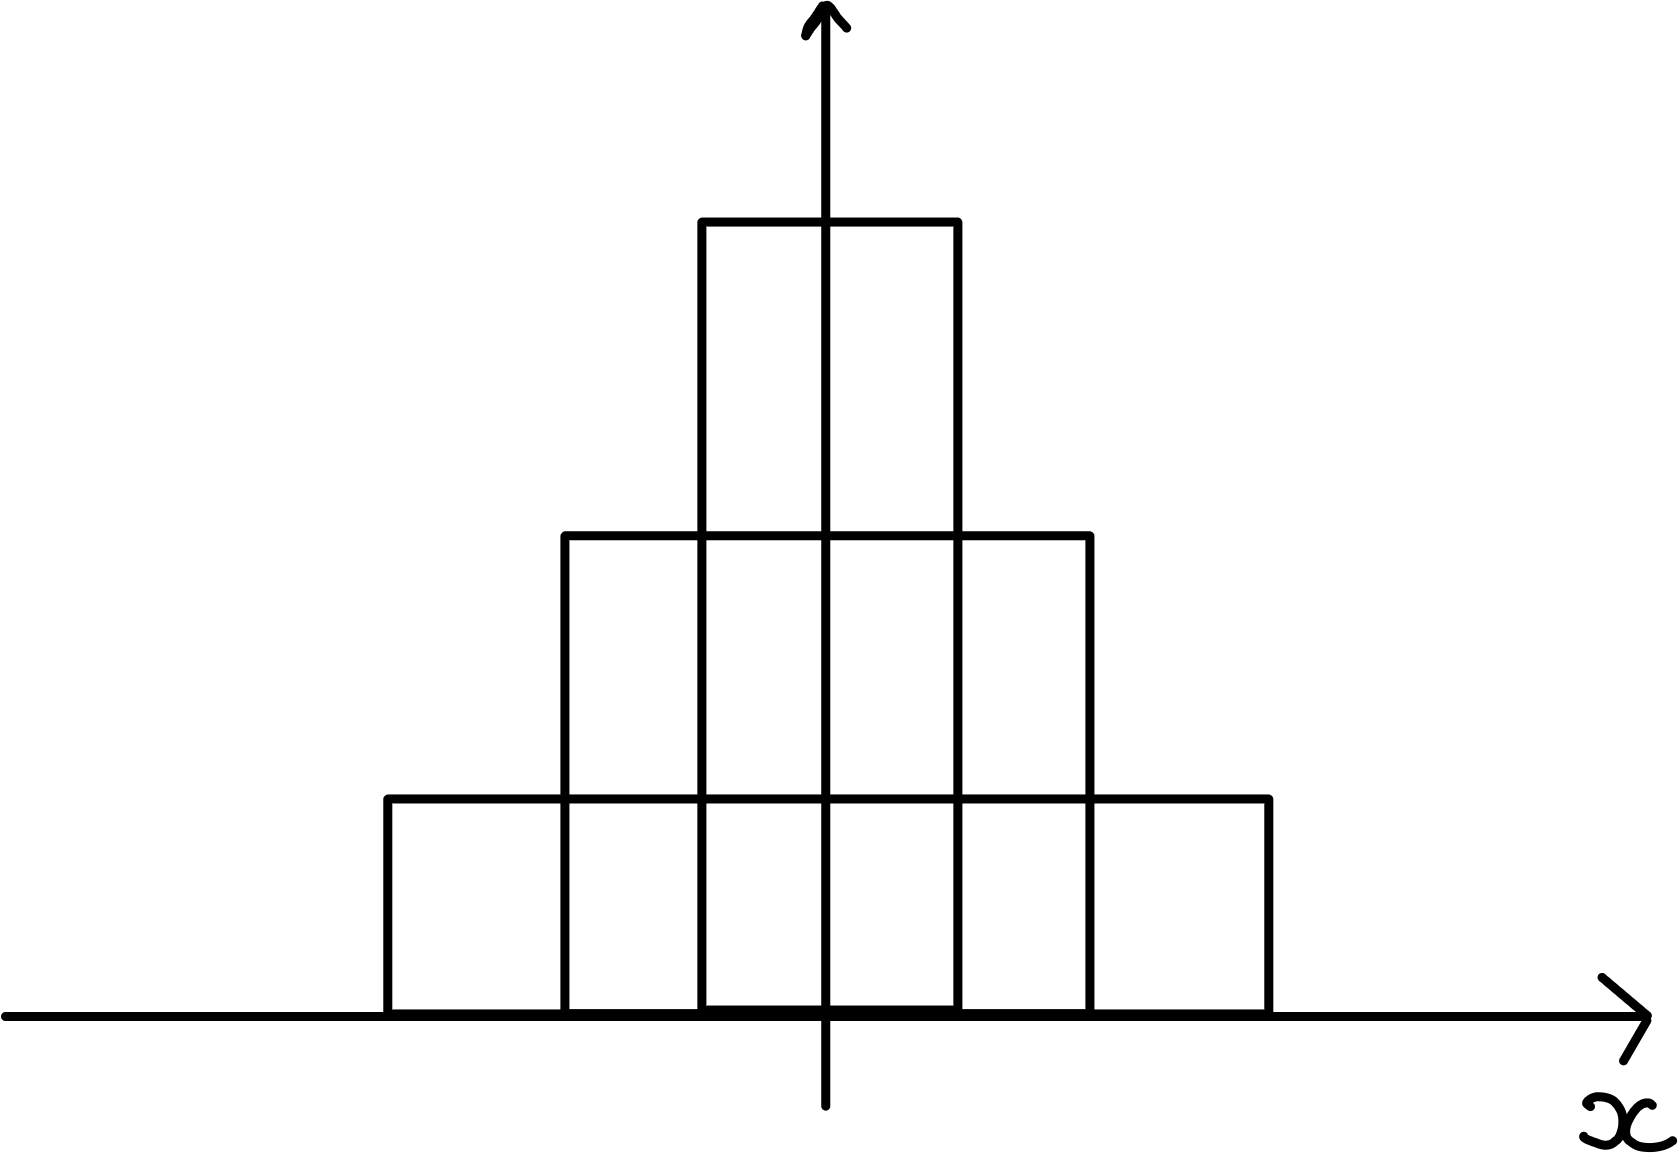
\includegraphics[height=5cm]{06-discretedelta} 
	\caption{Discrete approximation}
\end{figure}

\underline{Continuous:}
We can approximate the $\delta$ function using a Gaussian approximation as $\epsilon \to 0$.
\begin{align} \label{eq:6.3}
	\delta_\varepsilon(x) = \frac{1}{\varepsilon \sqrt{\pi}} \exp[-\frac{x^2}{\varepsilon^2}]
\end{align}
Therefore verifying \cref{eq:6.2},
\begin{align*}
	\int_{-\infty}^\infty f(x) \delta(x) \dd{x} & = \lim_{\varepsilon \to 0} \int_{-\infty}^\infty \frac{1}{\varepsilon \sqrt{\pi}} \exp[-\frac{x^2}{\varepsilon^2}] f(x) \dd{x}
	\intertext{Let $y = \frac{x}{\epsilon}$,}
    & = \lim_{\varepsilon \to 0} \int_{-\infty}^\infty \frac{1}{\sqrt{\pi}} \exp[-y^2] f(\varepsilon y) \dd{y} \\
    & = \lim_{\varepsilon \to 0} \int_{-\infty}^\infty \frac{1}{\sqrt{\pi}} \exp[-y^2] [f(0) + \varepsilon y f'(0) + \cdots] \dd{y} \\
    & = f(0)
\end{align*}
for all `well-behaved functions' $f$ at $0, \pm \infty$\footnote{Well behaved at $0$ lets us taylor expand and well behaved at $\pm \infty$ means it doesn't diverge faster than the Gaussian.}.
\begingroup
\tikzset{every picture/.style={scale=0.8}}
\begin{center}
	% Recommended preamble:
% \usetikzlibrary{arrows.meta}
% \usetikzlibrary{backgrounds}
% \usepgfplotslibrary{patchplots}
% \usepgfplotslibrary{fillbetween}
% \pgfplotsset{%
%     layers/standard/.define layer set={%
%         background,axis background,axis grid,axis ticks,axis lines,axis tick labels,pre main,main,axis descriptions,axis foreground%
%     }{
%         grid style={/pgfplots/on layer=axis grid},%
%         tick style={/pgfplots/on layer=axis ticks},%
%         axis line style={/pgfplots/on layer=axis lines},%
%         label style={/pgfplots/on layer=axis descriptions},%
%         legend style={/pgfplots/on layer=axis descriptions},%
%         title style={/pgfplots/on layer=axis descriptions},%
%         colorbar style={/pgfplots/on layer=axis descriptions},%
%         ticklabel style={/pgfplots/on layer=axis tick labels},%
%         axis background@ style={/pgfplots/on layer=axis background},%
%         3d box foreground style={/pgfplots/on layer=axis foreground},%
%     },
% }

\begin{tikzpicture}[/tikz/background rectangle/.style={fill={rgb,1:red,1.0;green,1.0;blue,1.0}, draw opacity={1.0}}, show background rectangle]
\begin{axis}[point meta max={nan}, point meta min={nan}, legend cell align={left}, legend columns={1}, title={}, title style={at={{(0.5,1)}}, anchor={south}, font={{\fontsize{14 pt}{18.2 pt}\selectfont}}, color={rgb,1:red,0.0;green,0.0;blue,0.0}, draw opacity={1.0}, rotate={0.0}, align={center}}, legend style={color={rgb,1:red,0.0;green,0.0;blue,0.0}, draw opacity={1.0}, line width={1}, solid, fill={rgb,1:red,1.0;green,1.0;blue,1.0}, fill opacity={1.0}, text opacity={1.0}, font={{\fontsize{8 pt}{10.4 pt}\selectfont}}, text={rgb,1:red,0.0;green,0.0;blue,0.0}, cells={anchor={center}}, at={(1.02, 1)}, anchor={north west}}, axis background/.style={fill={rgb,1:red,1.0;green,1.0;blue,1.0}, opacity={1.0}}, anchor={north west}, xshift={1.0mm}, yshift={-1.0mm}, width={145.4mm}, height={99.6mm}, scaled x ticks={false}, xlabel={$x$}, x tick style={color={rgb,1:red,0.0;green,0.0;blue,0.0}, opacity={1.0}}, x tick label style={color={rgb,1:red,0.0;green,0.0;blue,0.0}, opacity={1.0}, rotate={0}}, xlabel style={at={(ticklabel cs:0.5)}, anchor=near ticklabel, at={{(ticklabel cs:0.5)}}, anchor={near ticklabel}, font={{\fontsize{11 pt}{14.3 pt}\selectfont}}, color={rgb,1:red,0.0;green,0.0;blue,0.0}, draw opacity={1.0}, rotate={0.0}}, xmajorgrids={true}, xmin={-3.18}, xmax={3.18}, xticklabels={{$-3$,$-2$,$-1$,$0$,$1$,$2$,$3$}}, xtick={{-3.0,-2.0,-1.0,0.0,1.0,2.0,3.0}}, xtick align={inside}, xticklabel style={font={{\fontsize{8 pt}{10.4 pt}\selectfont}}, color={rgb,1:red,0.0;green,0.0;blue,0.0}, draw opacity={1.0}, rotate={0.0}}, x grid style={color={rgb,1:red,0.0;green,0.0;blue,0.0}, draw opacity={0.1}, line width={0.5}, solid}, axis x line*={left}, x axis line style={color={rgb,1:red,0.0;green,0.0;blue,0.0}, draw opacity={1.0}, line width={1}, solid}, scaled y ticks={false}, ylabel={$\delta_\varepsilon(x)$}, y tick style={color={rgb,1:red,0.0;green,0.0;blue,0.0}, opacity={1.0}}, y tick label style={color={rgb,1:red,0.0;green,0.0;blue,0.0}, opacity={1.0}, rotate={0}}, ylabel style={at={(ticklabel cs:0.5)}, anchor=near ticklabel, at={{(ticklabel cs:0.5)}}, anchor={near ticklabel}, font={{\fontsize{11 pt}{14.3 pt}\selectfont}}, color={rgb,1:red,0.0;green,0.0;blue,0.0}, draw opacity={1.0}, rotate={0.0}}, ymajorgrids={true}, ymin={-0.1354047167432424}, ymax={4.6488952748513235}, yticklabels={{$0$,$1$,$2$,$3$,$4$}}, ytick={{0.0,1.0,2.0,3.0,4.0}}, ytick align={inside}, yticklabel style={font={{\fontsize{8 pt}{10.4 pt}\selectfont}}, color={rgb,1:red,0.0;green,0.0;blue,0.0}, draw opacity={1.0}, rotate={0.0}}, y grid style={color={rgb,1:red,0.0;green,0.0;blue,0.0}, draw opacity={0.1}, line width={0.5}, solid}, axis y line*={left}, y axis line style={color={rgb,1:red,0.0;green,0.0;blue,0.0}, draw opacity={1.0}, line width={1}, solid}, colorbar={false}]
    \addplot[color={rgb,1:red,0.0;green,0.6056;blue,0.9787}, name path={9301c92f-18de-4450-ae5a-35afff11106c}, draw opacity={1.0}, line width={1}, solid]
        table[row sep={\\}]
        {
            \\
            -3.0  3.1687901131724237e-250  \\
            -2.9609367239208475  9.39781460355311e-244  \\
            -2.5997403313265086  6.293312116930993e-188  \\
            -2.3826763547775043  7.2292706182272e-158  \\
            -2.199151525136937  1.7029524963311301e-134  \\
            -1.9997921198677944  3.149477195036373e-111  \\
            -1.8160003818614874  9.796570654868876e-92  \\
            -1.6189562143740408  6.363369594192493e-73  \\
            -1.3906612226458708  7.961352563788823e-54  \\
            -1.1877795755559142  2.7604528396966285e-39  \\
            -1.00987065383912  2.0335438369458794e-28  \\
            -0.8159021733787222  1.4177079603549339e-18  \\
            -0.6207808849887516  8.774963089119262e-11  \\
            -0.5129151172455673  2.1988390791159464e-7  \\
            -0.40504934950238297  0.00012426653351608005  \\
            -0.3793914604421633  0.0004505922462812648  \\
            -0.3537335713819437  0.0015018170599526582  \\
            -0.3280756823217241  0.004601020214025313  \\
            -0.30241779326150453  0.012956718933280433  \\
            -0.28958884873139473  0.021066476676521728  \\
            -0.27675990420128493  0.033538197898531213  \\
            -0.26393095967117514  0.05228035000074701  \\
            -0.25110201514106534  0.07979729999477607  \\
            -0.24468754287601044  0.09780975191093307  \\
            -0.23827307061095554  0.11925836598538044  \\
            -0.23185859834590064  0.14464661959675607  \\
            -0.22544412608084574  0.1745180932892  \\
            -0.21902965381579084  0.20945241252217625  \\
            -0.21261518155073594  0.2500593001870305  \\
            -0.20620070928568104  0.29697055637461756  \\
            -0.19978623702062615  0.35082982805772434  \\
            -0.19311667417481276  0.4148896941616267  \\
            -0.18644711132899938  0.48786086723146954  \\
            -0.179777548483186  0.5704091975261611  \\
            -0.17310798563737262  0.6631385200082948  \\
            -0.16643842279155924  0.7665653624099615  \\
            -0.15976885994574586  0.8810921405607898  \\
            -0.15643407852283917  0.9426057726481537  \\
            -0.15309929709993247  1.0069795778232735  \\
            -0.14976451567702576  1.0742194972115524  \\
            -0.14642973425411906  1.144319235495385  \\
            -0.13976017140830568  1.2930071712466085  \\
            -0.1330906085624923  1.452719842937036  \\
            -0.12642104571667892  1.6228934357221645  \\
            -0.11975148287086554  1.8027078023619365  \\
            -0.11308192002505216  1.9910761630477771  \\
            -0.10641235717923878  2.1866416071706682  \\
            -0.0997427943334254  2.387781273641675  \\
            -0.093073231487612  2.5926188605085754  \\
            -0.0864036686417986  2.7990458343279454  \\
            -0.07973410579598522  3.004751384501715  \\
            -0.07306454295017184  3.2072608106018317  \\
            -0.06639498010435846  3.403981657691705  \\
            -0.05972541725854508  3.5922565442186114  \\
            -0.053055854412731696  3.769421278914807  \\
            -0.049721072989825005  3.8530180581228444  \\
            -0.046386291566918314  3.932866557163835  \\
            -0.04305151014401162  4.008659584009742  \\
            -0.03971672872110493  4.080101282195823  \\
            -0.03638194729819824  4.146909048087371  \\
            -0.03304716587529155  4.20881538861213  \\
            -0.02971238445238486  4.265569702415517  \\
            -0.026377603029478166  4.316939967872759  \\
            -0.02304282160657147  4.3627143220667  \\
            -0.01970804018366478  4.402702515706628  \\
            -0.01637325876075809  4.43673723001371  \\
            -0.0130384773378514  4.464675242821175  \\
            -0.009703695914944709  4.486398432518669  \\
            -0.006368914492038016  4.501814609993881  \\
            -0.003034133069131324  4.510858170372357  \\
            0.0003006483537753681  4.5134905581080815  \\
            0.00363542977668206  4.5097005408109965  \\
            0.006970211199588752  4.499504289090081  \\
            0.010304992622495443  4.482945261617806  \\
            0.013639774045402136  4.460093896559111  \\
            0.016446949680120546  4.436050532649423  \\
            0.019254125314838957  4.407688634459925  \\
            0.02206130094955737  4.37509281648702  \\
            0.02486847658427578  4.33835987017029  \\
            0.027675652218994193  4.297598285088465  \\
            0.030482827853712605  4.252927715223899  \\
            0.033290003488431016  4.204478393969637  \\
            0.03609717912314943  4.152390501880297  \\
            0.03890435475786784  4.096813491460039  \\
            0.04171153039258625  4.037905373535479  \\
            0.044518706027304664  3.975831969976599  \\
            0.047325881662023075  3.910766137703177  \\
            0.0529402329314599  3.772378973628859  \\
            0.05855458420089672  3.624236630985895  \\
            0.06416893547033355  3.467891779126281  \\
            0.06978328673977037  3.3049301678273997  \\
            0.0753976380092072  3.1369442410579933  \\
            0.08101198927864402  2.9655078064457685  \\
            0.09224069181751766  2.6183451713407653  \\
            0.10346939435639131  2.274813343838524  \\
            0.10908374562582812  2.1075449324561104  \\
            0.11469809689526494  1.9447137211070167  \\
            0.12031244816470177  1.7872375274579795  \\
            0.1259267994341386  1.635899546742392  \\
            0.13154115070357542  1.4913471540850294  \\
            0.13715550197301224  1.354093421221986  \\
            0.14276985324244906  1.224521083222509  \\
            0.1483842045118859  1.1028886478129494  \\
            0.1539985557813227  0.9893383101111929  \\
            0.15961290705075953  0.8839053188399951  \\
            0.16522725832019636  0.7865284357532991  \\
            0.17084160958963318  0.6970611370233241  \\
            0.17645596085907  0.6152832223133685  \\
            0.18207031212850683  0.540912522581052  \\
            0.18768466339794365  0.4736164295543675  \\
            0.19329901466738048  0.41302300647863943  \\
            0.20015350120732034  0.3475472888688286  \\
            0.20700798774726023  0.2906977972981577  \\
            0.21386247428720012  0.24168948238753776  \\
            0.22071696082713999  0.19973857025202604  \\
            0.22757144736707985  0.1640794897023623  \\
            0.2344259339070197  0.1339784136076442  \\
            0.24128042044695958  0.10874355839981903  \\
            0.24813490698689947  0.08773248361983058  \\
            0.2618438800667792  0.05608396573600284  \\
            0.27555285314665895  0.03500013384385919  \\
            0.28926182622653873  0.021323249741359636  \\
            0.30297079930641846  0.012682059321306555  \\
            0.33038874546617797  0.004173694427288526  \\
            0.3578066916259375  0.001247562501897781  \\
            0.38522463778569693  0.00033869966713932266  \\
            0.41264258394545644  8.351760293801774e-5  \\
            0.513108876864534  2.1710397507607256e-7  \\
            0.6135751697836116  1.5504732924613018e-10  \\
            0.7991519189555105  8.007717307674473e-18  \\
            0.9871354150600441  3.717119866523065e-27  \\
            1.1978122140406555  5.9668426120590896e-40  \\
            1.388719406219134  1.1245970773344658e-53  \\
            1.6072949743767582  7.069478227687967e-72  \\
            1.8096765128752679  4.2497444897081354e-91  \\
            2.009200994923107  2.8171737950880423e-112  \\
            2.202922753671847  5.885372290691178e-135  \\
            2.4015123274889874  2.2613412180743035e-160  \\
            2.6190902607646405  9.818482143595239e-191  \\
            2.93515789239279  1.576481105264437e-239  \\
            3.0  3.1687901131724237e-250  \\
        }
        ;
    \addlegendentry {$ε = 2^{-3}$}
    \addplot[color={rgb,1:red,0.8889;green,0.4356;blue,0.2781}, name path={c21cbeaa-296f-451f-bd6a-41d8ce7bbebc}, draw opacity={1.0}, line width={1}, solid]
        table[row sep={\\}]
        {
            \\
            -3.0  6.532503647797609e-63  \\
            -2.9609367239208475  2.7108969603874276e-61  \\
            -2.5997403313265086  2.4523141841736653e-47  \\
            -2.3826763547775043  8.028416833972961e-40  \\
            -2.199151525136937  5.59315591241414e-34  \\
            -1.9997921198677944  3.667886677676559e-28  \\
            -1.8160003818614874  2.739206736675871e-23  \\
            -1.6189562143740408  1.3828595696209478e-18  \\
            -1.3906612226458708  8.22437693647071e-14  \\
            -1.1877795755559142  3.548962213099155e-10  \\
            -1.00987065383912  1.8489266275542406e-7  \\
            -0.9128864136089211  3.6533856380411288e-6  \\
            -0.8159021733787222  5.3426040225238017e-5  \\
            -0.7671218512812296  0.00018379573787953506  \\
            -0.718341529183737  0.0005859339883465548  \\
            -0.6695612070862442  0.0017309827946840215  \\
            -0.6207808849887516  0.004738791675832074  \\
            -0.5938144430529555  0.00800314998834751  \\
            -0.5668480011171595  0.013205299090033602  \\
            -0.5398815591813634  0.02128773595372286  \\
            -0.5129151172455673  0.033527768877876  \\
            -0.49943189627766926  0.041711179769700395  \\
            -0.4859486753097712  0.05159098028925014  \\
            -0.47246545434187315  0.06344078863434087  \\
            -0.45898223337397515  0.07755983076081178  \\
            -0.4454990124060771  0.09427110964857881  \\
            -0.43201579143817903  0.11391839882946726  \\
            -0.41853257047028103  0.13686191481366292  \\
            -0.40504934950238297  0.16347255038032008  \\
            -0.3922204049722732  0.1925383125101431  \\
            -0.3793914604421633  0.22558084589558128  \\
            -0.3665625159120535  0.26290570927544793  \\
            -0.3537335713819437  0.30479690355339456  \\
            -0.3409046268518339  0.351506872659441  \\
            -0.3280756823217241  0.4032457767357382  \\
            -0.31524673779161433  0.46017028518452024  \\
            -0.30241779326150453  0.5223721945981948  \\
            -0.28958884873139473  0.5898672291426873  \\
            -0.27675990420128493  0.6625844251972072  \\
            -0.26393095967117514  0.740356534547053  \\
            -0.25110201514106534  0.8229118979356298  \\
            -0.23827307061095554  0.9098682404590356  \\
            -0.22544412608084574  1.0007288199057438  \\
            -0.21261518155073594  1.0948813173160676  \\
            -0.19978623702062615  1.1915997953932551  \\
            -0.17310798563737262  1.3971960727303163  \\
            -0.14642973425411906  1.601375175864644  \\
            -0.1330906085624923  1.6998153997686394  \\
            -0.11975148287086554  1.7940627411561616  \\
            -0.11308192002505216  1.8391970454076139  \\
            -0.10641235717923878  1.8827848463136836  \\
            -0.0997427943334254  1.9246640207897956  \\
            -0.093073231487612  1.9646760967652295  \\
            -0.0864036686417986  2.002667245688309  \\
            -0.07973410579598522  2.038489263013643  \\
            -0.07306454295017184  2.0720005279739997  \\
            -0.06639498010435846  2.1030669339731616  \\
            -0.05972541725854508  2.1315627810699223  \\
            -0.053055854412731696  2.1573716222573904  \\
            -0.046386291566918314  2.180387055574678  \\
            -0.03971672872110493  2.2005134545171066  \\
            -0.03304716587529155  2.2176666297321503  \\
            -0.026377603029478166  2.2317744155958645  \\
            -0.01970804018366478  2.2427771759517907  \\
            -0.0130384773378514  2.2506282240531252  \\
            -0.006368914492038016  2.255294152570284  \\
            0.0003006483537753681  2.256755070399699  \\
            0.006970211199588752  2.255004743924887  \\
            0.013639774045402136  2.250050641325983  \\
            0.019254125314838957  2.2434119001468  \\
            0.02486847658427578  2.23453769803537  \\
            0.030482827853712605  2.2234547356111407  \\
            0.03609717912314943  2.210196259399388  \\
            0.04171153039258625  2.1948018956702997  \\
            0.047325881662023075  2.1773174531274493  \\
            0.0529402329314599  2.157794695820574  \\
            0.05855458420089672  2.136291087858008  \\
            0.06416893547033355  2.1128695116804703  \\
            0.06978328673977037  2.0875979618286604  \\
            0.0753976380092072  2.060549216290819  \\
            0.08101198927864402  2.0318004876518745  \\
            0.08662634054808084  2.0014330563819547  \\
            0.09224069181751766  1.9695318886981033  \\
            0.09785504308695449  1.936185241508368  \\
            0.10346939435639131  1.901484257001622  \\
            0.11469809689526494  1.8283957870374044  \\
            0.1259267994341386  1.7510375135454417  \\
            0.13715550197301224  1.6701998846137278  \\
            0.1483842045118859  1.5866794937157722  \\
            0.17084160958963318  1.4147314556915325  \\
            0.19329901466738048  1.2412231106901714  \\
            0.20700798774726023  1.1368855002785407  \\
            0.22071696082713999  1.0350748981349687  \\
            0.2344259339070197  0.9367312311771446  \\
            0.24813490698689947  0.8426483957719927  \\
            0.2618438800667792  0.7534700102840881  \\
            0.27555285314665895  0.6696898529332199  \\
            0.2824073396865988  0.6299385084806262  \\
            0.28926182622653873  0.591656500823318  \\
            0.2961163127664786  0.5548660682714782  \\
            0.30297079930641846  0.5195815694201555  \\
            0.3098252858463583  0.48580988934316116  \\
            0.3166797723862982  0.4535508745804794  \\
            0.3235342589262381  0.422797791297742  \\
            0.33038874546617797  0.3935378011219317  \\
            0.33724323200611783  0.365752449338727  \\
            0.34409771854605775  0.3394181603677886  \\
            0.3509522050859976  0.3145067357064409  \\
            0.3578066916259375  0.2909858498431189  \\
            0.3715156647058172  0.2479686857928801  \\
            0.38522463778569693  0.2100438571036372  \\
            0.39893361086557666  0.17685254090600896  \\
            0.41264258394545644  0.14801331912672744  \\
            0.42520087056034117  0.12507983481737658  \\
            0.43775915717522584  0.10516761620100935  \\
            0.4503174437901105  0.08798020924749983  \\
            0.4628757304049952  0.0732312050342449  \\
            0.47543401701987986  0.06064787662928307  \\
            0.4879923036347646  0.04997390067616607  \\
            0.5005505902496493  0.04097124186992212  \\
            0.513108876864534  0.03342129210016576  \\
            0.5382254500943033  0.02190464106419405  \\
            0.5633420233240728  0.014069606920156238  \\
            0.5884585965538423  0.00885647101039307  \\
            0.6135751697836116  0.005463517830428291  \\
            0.6599693570765863  0.0021227912726021004  \\
            0.7063635443695611  0.0007698907850036368  \\
            0.7527577316625358  0.000260638068680944  \\
            0.7991519189555105  8.236325006182906e-5  \\
            0.8931436670077773  6.463365888678688e-6  \\
            0.9871354150600441  3.823032005475622e-7  \\
            1.1978122140406555  2.419872242587979e-10  \\
            1.388719406219134  8.966140292320151e-14  \\
            1.6072949743767582  2.5246613567124797e-18  \\
            1.8096765128752679  3.953183710873427e-23  \\
            2.009200994923107  2.0059019581202498e-28  \\
            2.202922753671847  4.288444336583017e-34  \\
            2.4015123274889874  1.898662693160747e-40  \\
            2.6190902607646405  4.8737963792137843e-48  \\
            2.93515789239279  3.0851656321409415e-60  \\
            3.0  6.532503647797609e-63  \\
        }
        ;
    \addlegendentry {$ε = 2^{-2}$}
    \addplot[color={rgb,1:red,0.2422;green,0.6433;blue,0.3044}, name path={a532c86f-34d5-401a-a2f8-fbea3ee3ae0c}, draw opacity={1.0}, line width={1}, solid]
        table[row sep={\\}]
        {
            \\
            -3.0  2.617301239249265e-16  \\
            -2.9609367239208475  6.642966284232493e-16  \\
            -2.5997403313265086  2.0486974321776623e-12  \\
            -2.3826763547775043  1.5496773083759404e-10  \\
            -2.199151525136937  4.4771127021678465e-9  \\
            -1.9997921198677944  1.274053815791314e-7  \\
            -1.8160003818614874  2.1061533944186058e-6  \\
            -1.6189562143740408  3.1570271401773835e-5  \\
            -1.3906612226458708  0.0004930143351068951  \\
            -1.2892203991008926  0.0014625486533025077  \\
            -1.1877795755559142  0.003995849654926455  \\
            -1.1433023451267155  0.006049505342491231  \\
            -1.098825114697517  0.009014829881361682  \\
            -1.0543478842683185  0.013222761125996624  \\
            -1.00987065383912  0.019090342266493098  \\
            -0.9856245937815703  0.02316665956020944  \\
            -0.9613785337240206  0.027981477577716036  \\
            -0.9371324736664708  0.03363840512206885  \\
            -0.9128864136089211  0.04024923912705927  \\
            -0.8886403535513714  0.047933316468420556  \\
            -0.8643942934938216  0.05681654327252581  \\
            -0.8401482334362719  0.06703006834805664  \\
            -0.8159021733787222  0.07870857365915374  \\
            -0.7915120123299759  0.09207214494911897  \\
            -0.7671218512812296  0.1071933033317097  \\
            -0.7427316902324832  0.12420532735226801  \\
            -0.718341529183737  0.14323394985453056  \\
            -0.6939513681349906  0.16439359323483554  \\
            -0.6695612070862442  0.18778330714435104  \\
            -0.645171046037498  0.21348248717841992  \\
            -0.6207808849887516  0.2415464726583744  \\
            -0.6072976640208536  0.2580867337408062  \\
            -0.5938144430529555  0.2753588470813796  \\
            -0.5803312220850575  0.2933599071654701  \\
            -0.5668480011171595  0.3120835346184055  \\
            -0.5398815591813634  0.3516544878165147  \\
            -0.5129151172455673  0.3939444252252405  \\
            -0.4859486753097712  0.43876021496303963  \\
            -0.45898223337397515  0.4858397098643159  \\
            -0.43201579143817903  0.5348503244708183  \\
            -0.40504934950238297  0.5853896035231857  \\
            -0.3537335713819437  0.6840477728467939  \\
            -0.30241779326150453  0.7826702181130658  \\
            -0.27675990420128493  0.8306041589298587  \\
            -0.25110201514106534  0.8768435889087651  \\
            -0.23827307061095554  0.8991422846901173  \\
            -0.22544412608084574  0.9207948833793353  \\
            -0.21261518155073594  0.9417281595091707  \\
            -0.19978623702062615  0.9618700463688094  \\
            -0.18644711132899938  0.9818979823452749  \\
            -0.17310798563737262  1.000917159203043  \\
            -0.15976885994574586  1.0188534059570384  \\
            -0.14642973425411906  1.0356358328408293  \\
            -0.1330906085624923  1.0511972968814627  \\
            -0.11975148287086554  1.0654748486148982  \\
            -0.10641235717923878  1.0784101557909305  \\
            -0.093073231487612  1.0899499000818593  \\
            -0.07973410579598522  1.1000461430226183  \\
            -0.06639498010435846  1.108656657669609  \\
            -0.053055854412731696  1.1157452227683253  \\
            -0.03971672872110493  1.121281876562594  \\
            -0.026377603029478166  1.1252431277569246  \\
            -0.0130384773378514  1.1276121215534636  \\
            0.0003006483537753681  1.1283787591213756  \\
            0.013639774045402136  1.127539769313673  \\
            0.02486847658427578  1.1255912724766708  \\
            0.03609717912314943  1.1225133259931799  \\
            0.047325881662023075  1.1183152160096705  \\
            0.05855458420089672  1.1130095807653564  \\
            0.06978328673977037  1.1066123472024472  \\
            0.08101198927864402  1.099142651309606  \\
            0.09224069181751766  1.0906227427561608  \\
            0.10346939435639131  1.0810778744821823  \\
            0.11469809689526494  1.07053617801115  \\
            0.1259267994341386  1.0590285253466782  \\
            0.13715550197301224  1.046588378401896  \\
            0.1483842045118859  1.033251626988803  \\
            0.15961290705075953  1.0190564164646698  \\
            0.17084160958963318  1.0040429661927324  \\
            0.18207031212850683  0.988253380024656  \\
            0.19329901466738048  0.9717314500521467  \\
            0.20700798774726023  0.9506331997835771  \\
            0.22071696082713999  0.928595852737249  \\
            0.2344259339070197  0.9057066272881538  \\
            0.24813490698689947  0.8820544496124538  \\
            0.27555285314665895  0.8328220693321566  \\
            0.30297079930641846  0.7816228191133114  \\
            0.3578066916259375  0.6761635619529811  \\
            0.41264258394545644  0.5710300917052741  \\
            0.43775915717522584  0.5242691501916592  \\
            0.4628757304049952  0.47891433947534506  \\
            0.4879923036347646  0.43528089703145695  \\
            0.513108876864534  0.3936312819616734  \\
            0.5382254500943033  0.35417494150272855  \\
            0.5633420233240728  0.3170693677492819  \\
            0.5884585965538423  0.28242229115391515  \\
            0.6135751697836116  0.2502948344319125  \\
            0.636772263430099  0.22287740227971747  \\
            0.6599693570765863  0.19761077387712192  \\
            0.6831664507230737  0.17445588803290002  \\
            0.7063635443695611  0.1533525761175881  \\
            0.7295606380160484  0.1342230030339914  \\
            0.7527577316625358  0.11697505492611515  \\
            0.7759548253090232  0.1015055983314776  \\
            0.7991519189555105  0.08770354832240959  \\
            0.8226498559685772  0.07530348193074325  \\
            0.8461477929816439  0.06437164018665043  \\
            0.8696457299947106  0.05478424944888236  \\
            0.8931436670077773  0.04641928867032293  \\
            0.9166416040208439  0.039158213485873776  \\
            0.9401395410339106  0.03288735015795745  \\
            0.9636374780469774  0.02749897579691534  \\
            0.9871354150600441  0.022892107624872673  \\
            1.039804614805197  0.014935829170435485  \\
            1.0924738145503499  0.009530921186095772  \\
            1.1451430142955026  0.005948430622595685  \\
            1.1978122140406555  0.0036310472895996586  \\
            1.2932658101298946  0.0014026898210219914  \\
            1.388719406219134  0.0005037733370112364  \\
            1.6072949743767582  3.6697339416610036e-5  \\
            1.8096765128752679  2.3084503853856095e-6  \\
            2.009200994923107  1.095623203067123e-7  \\
            2.202922753671847  4.189466672366105e-9  \\
            2.4015123274889874  1.0806766051757937e-10  \\
            2.6190902607646405  1.3678883186240157e-12  \\
            2.93515789239279  1.2201224461958778e-15  \\
            3.0  2.617301239249265e-16  \\
        }
        ;
    \addlegendentry {$ε = 2^{-1}$}
    \addplot[color={rgb,1:red,0.7644;green,0.4441;blue,0.8243}, name path={3d3b8db3-3875-4af1-b985-df233926b873}, draw opacity={1.0}, line width={1}, solid]
        table[row sep={\\}]
        {
            \\
            -3.0  6.962652597337395e-5  \\
            -2.9804683619604235  7.825353142176361e-5  \\
            -2.9609367239208475  8.788238021458185e-5  \\
            -2.780338527623678  0.0002478598057309385  \\
            -2.5997403313265086  0.00065490869221132  \\
            -2.4912083430520067  0.0011379988527388208  \\
            -2.3826763547775043  0.0019313972881056679  \\
            -2.2909139399572207  0.0029656720142803637  \\
            -2.199151525136937  0.004477759929072768  \\
            -2.0994718225023656  0.006873052994034807  \\
            -1.9997921198677944  0.010342088314832028  \\
            -1.9078962508646409  0.014810290333855728  \\
            -1.8160003818614874  0.020853732502639676  \\
            -1.7667393399896256  0.024878959359024413  \\
            -1.717478298117764  0.029537440601296816  \\
            -1.6682172562459026  0.03489841881497424  \\
            -1.6189562143740408  0.04103277394919611  \\
            -1.5618824664419981  0.04920097778986362  \\
            -1.5048087185099557  0.05861209395382674  \\
            -1.4477349705779132  0.06936995099885265  \\
            -1.3906612226458708  0.08156919674941943  \\
            -1.3399408108733817  0.09368601820811569  \\
            -1.2892203991008926  0.10705054419689662  \\
            -1.2384999873284035  0.12169380775138758  \\
            -1.1877795755559142  0.13763015014866012  \\
            -1.1433023451267155  0.15266562674138  \\
            -1.098825114697517  0.16867498597533834  \\
            -1.0543478842683185  0.1856272953488789  \\
            -1.00987065383912  0.2034767196475148  \\
            -0.9613785337240206  0.223887042688019  \\
            -0.9128864136089211  0.2451888504807545  \\
            -0.8643942934938216  0.2672575610177068  \\
            -0.8159021733787222  0.2899457914674334  \\
            -0.718341529183737  0.3367617757529399  \\
            -0.6207808849887516  0.383761562557319  \\
            -0.5668480011171595  0.40914666245985226  \\
            -0.5129151172455673  0.43368064341086626  \\
            -0.4859486753097712  0.44552092745808314  \\
            -0.45898223337397515  0.457019310764875  \\
            -0.43201579143817903  0.4681331162970862  \\
            -0.40504934950238297  0.4788202952497445  \\
            -0.3793914604421633  0.4885551959575023  \\
            -0.3537335713819437  0.49783211242185793  \\
            -0.3280756823217241  0.5066177035268725  \\
            -0.30241779326150453  0.5148799745506462  \\
            -0.27675990420128493  0.5225884707336694  \\
            -0.25110201514106534  0.5297144639203194  \\
            -0.22544412608084574  0.5362311306762859  \\
            -0.19978623702062615  0.5421137203388033  \\
            -0.17310798563737262  0.5475336721076567  \\
            -0.14642973425411906  0.5522211880375654  \\
            -0.11975148287086554  0.5561566050821904  \\
            -0.093073231487612  0.5593233276647973  \\
            -0.06639498010435846  0.5617079442556648  \\
            -0.03971672872110493  0.5633003219916456  \\
            -0.0130384773378514  0.5640936784037662  \\
            0.013639774045402136  0.5640846295423769  \\
            0.03609717912314943  0.563454919682847  \\
            0.05855458420089672  0.5622584933491559  \\
            0.08101198927864402  0.5604989637139971  \\
            0.10346939435639131  0.558181635179785  \\
            0.1259267994341386  0.5553134767359842  \\
            0.1483842045118859  0.55190308704106  \\
            0.17084160958963318  0.5479606514739062  \\
            0.19329901466738048  0.543497891454965  \\
            0.22071696082713999  0.5373632769935863  \\
            0.24813490698689947  0.5304997060701915  \\
            0.27555285314665895  0.5229369807883504  \\
            0.30297079930641846  0.514707630054979  \\
            0.33038874546617797  0.5058466767154356  \\
            0.3578066916259375  0.4963913895970638  \\
            0.38522463778569693  0.4863810229140504  \\
            0.41264258394545644  0.4758565455777577  \\
            0.4628757304049952  0.45538189394277423  \\
            0.513108876864534  0.43359443539317166  \\
            0.5633420233240728  0.41077109004719264  \\
            0.6135751697836116  0.38719012330447605  \\
            0.7063635443695611  0.34255796328191324  \\
            0.7991519189555105  0.297896629807229  \\
            0.8461477929816439  0.27573058522420135  \\
            0.8931436670077773  0.2540890322173566  \\
            0.9401395410339106  0.23311408745127576  \\
            0.9871354150600441  0.21292798466826043  \\
            1.039804614805197  0.19136769824711208  \\
            1.0924738145503499  0.17103894867209235  \\
            1.1451430142955026  0.15202391026764628  \\
            1.1978122140406555  0.1343752468565796  \\
            1.245539012085275  0.1195844606537621  \\
            1.2932658101298946  0.10593798549484941  \\
            1.3409926081745143  0.09342221462253296  \\
            1.388719406219134  0.08201061965345743  \\
            1.44336329825854  0.07025227733704982  \\
            1.4980071902979462  0.05982148000526454  \\
            1.552651082337352  0.05063610971817858  \\
            1.6072949743767582  0.04260591960138823  \\
            1.6578903590013856  0.036117947179541934  \\
            1.708485743626013  0.030461597742526946  \\
            1.7590811282506404  0.025559879632634452  \\
            1.8096765128752679  0.021337396869379504  \\
            1.8595576333872277  0.017768651343759368  \\
            1.9094387538991873  0.014723339873807988  \\
            1.959319874411147  0.012139395202251348  \\
            2.009200994923107  0.009959249307842357  \\
            2.106061874297477  0.006685183887720753  \\
            2.202922753671847  0.004404037251619891  \\
            2.3022175405804175  0.002815626323588246  \\
            2.4015123274889874  0.0017649614997523278  \\
            2.5103012941268137  0.0010343546945692393  \\
            2.6190902607646405  0.0005920030701929997  \\
            2.7771240765787155  0.0002523274069904906  \\
            2.93515789239279  0.00010230860264657333  \\
            2.967578946196395  8.448895477786285e-5  \\
            3.0  6.962652597337395e-5  \\
        }
        ;
    \addlegendentry {$ε = 2^{0}$}
\end{axis}
\end{tikzpicture}

\end{center} 
\endgroup

\underline{Further Examples}
We could alternatively use the Dirichlet kernel (as $n \to \infty$)
\begin{align} \label{eq:6.4}
	\delta_n(x) = \frac{\sin n x}{\pi x} = \frac{1}{2\pi} \int_{-n}^n e^{ikx} \dd{k}
\end{align}
or even
\begin{align} \label{eq:6.5}
	\delta_n(x) = \frac{n}{2} \sech^2 nx
\end{align}

\subsection{Integral and derivative of delta function}
\subsubsection{Integral of $\delta(x)$}
We define the Heaviside step function by
\begin{align} \label{eq:6.6}
	H(x) = \begin{cases}
		1 & x \geq 0 \\
		0 & x < 0
	\end{cases}
\end{align}
For $x \neq 0$, we have
\begin{align} \label{eq:6.7}
	H(x) = \int_{-\infty}^x \delta(t) \dd{t}
\end{align}
Thus,
\begin{align*}
	\dv{x} H(x) = \delta(x)
\end{align*}
where this identification takes place under an implied integral.

\begin{exercise}
	Verify using \cref{eq:6.5} $\delta(x) = \lim_{n \to \infty} \frac{n}{2} \sech^2 nx$ [You will find $\frac{1}{2} (\tanh nx + 1)$ which is an approximate step function. This also gives $H(0) = \frac{1}{2}$ (an alternative definition)].
\end{exercise} 

\subsubsection{Derivative of $\delta(x)$}
We define $\delta'(x)$ using integration by parts.
\begin{align}
	\int_{-\infty}^\infty \delta'(x-\xi) f(x) \dd{x} &= \qty[\delta(x-\xi) f(x)]_{-\infty}^\infty - \int_{-\infty}^\infty \delta(x-\xi) f'(x) \dd{x} \notag \\
    &= - \int_{-\infty}^\infty \delta(x-\xi) f'(x) \dd{x} \notag \\
    \int_{-\infty}^\infty \delta'(x-\xi) f(x) \dd{x} &= - f'(\xi) \label{eq:6.8}
\end{align}
This is valid for all $f$ that are smooth at $x = \xi$.
\begin{example}
	Consider the Gaussian approximation \cref{eq:6.3}:
	\begin{align*}
		\delta_\varepsilon(x) = \frac{1}{\varepsilon \sqrt{\pi}} \exp[-\frac{x^2}{\varepsilon^2}]
	\end{align*}
	Then,
	\begin{align*}
		\delta_\varepsilon'(x) = \frac{-2x}{\varepsilon^3 \sqrt{\pi}} \exp[-\frac{x^2}{\varepsilon^2}]
	\end{align*}

	\begingroup
	\tikzset{every picture/.style={scale=0.8}}
	\begin{center}
		% Recommended preamble:
% \usetikzlibrary{arrows.meta}
% \usetikzlibrary{backgrounds}
% \usepgfplotslibrary{patchplots}
% \usepgfplotslibrary{fillbetween}
% \pgfplotsset{%
%     layers/standard/.define layer set={%
%         background,axis background,axis grid,axis ticks,axis lines,axis tick labels,pre main,main,axis descriptions,axis foreground%
%     }{
%         grid style={/pgfplots/on layer=axis grid},%
%         tick style={/pgfplots/on layer=axis ticks},%
%         axis line style={/pgfplots/on layer=axis lines},%
%         label style={/pgfplots/on layer=axis descriptions},%
%         legend style={/pgfplots/on layer=axis descriptions},%
%         title style={/pgfplots/on layer=axis descriptions},%
%         colorbar style={/pgfplots/on layer=axis descriptions},%
%         ticklabel style={/pgfplots/on layer=axis tick labels},%
%         axis background@ style={/pgfplots/on layer=axis background},%
%         3d box foreground style={/pgfplots/on layer=axis foreground},%
%     },
% }

\begin{tikzpicture}[/tikz/background rectangle/.style={fill={rgb,1:red,1.0;green,1.0;blue,1.0}, draw opacity={1.0}}, show background rectangle]
\begin{axis}[point meta max={nan}, point meta min={nan}, legend cell align={left}, legend columns={1}, title={}, title style={at={{(0.5,1)}}, anchor={south}, font={{\fontsize{14 pt}{18.2 pt}\selectfont}}, color={rgb,1:red,0.0;green,0.0;blue,0.0}, draw opacity={1.0}, rotate={0.0}, align={center}}, legend style={color={rgb,1:red,0.0;green,0.0;blue,0.0}, draw opacity={1.0}, line width={1}, solid, fill={rgb,1:red,1.0;green,1.0;blue,1.0}, fill opacity={1.0}, text opacity={1.0}, font={{\fontsize{8 pt}{10.4 pt}\selectfont}}, text={rgb,1:red,0.0;green,0.0;blue,0.0}, cells={anchor={center}}, at={(1.02, 1)}, anchor={north west}}, axis background/.style={fill={rgb,1:red,1.0;green,1.0;blue,1.0}, opacity={1.0}}, anchor={north west}, xshift={1.0mm}, yshift={-1.0mm}, width={145.4mm}, height={99.6mm}, scaled x ticks={false}, xlabel={$x$}, x tick style={color={rgb,1:red,0.0;green,0.0;blue,0.0}, opacity={1.0}}, x tick label style={color={rgb,1:red,0.0;green,0.0;blue,0.0}, opacity={1.0}, rotate={0}}, xlabel style={at={(ticklabel cs:0.5)}, anchor=near ticklabel, at={{(ticklabel cs:0.5)}}, anchor={near ticklabel}, font={{\fontsize{11 pt}{14.3 pt}\selectfont}}, color={rgb,1:red,0.0;green,0.0;blue,0.0}, draw opacity={1.0}, rotate={0.0}}, xmajorgrids={true}, xmin={-3.18}, xmax={3.18}, xticklabels={{$-3$,$-2$,$-1$,$0$,$1$,$2$,$3$}}, xtick={{-3.0,-2.0,-1.0,0.0,1.0,2.0,3.0}}, xtick align={inside}, xticklabel style={font={{\fontsize{8 pt}{10.4 pt}\selectfont}}, color={rgb,1:red,0.0;green,0.0;blue,0.0}, draw opacity={1.0}, rotate={0.0}}, x grid style={color={rgb,1:red,0.0;green,0.0;blue,0.0}, draw opacity={0.1}, line width={0.5}, solid}, axis x line*={left}, x axis line style={color={rgb,1:red,0.0;green,0.0;blue,0.0}, draw opacity={1.0}, line width={1}, solid}, scaled y ticks={false}, ylabel={$\delta'_\varepsilon(x)$}, y tick style={color={rgb,1:red,0.0;green,0.0;blue,0.0}, opacity={1.0}}, y tick label style={color={rgb,1:red,0.0;green,0.0;blue,0.0}, opacity={1.0}, rotate={0}}, ylabel style={at={(ticklabel cs:0.5)}, anchor=near ticklabel, at={{(ticklabel cs:0.5)}}, anchor={near ticklabel}, font={{\fontsize{11 pt}{14.3 pt}\selectfont}}, color={rgb,1:red,0.0;green,0.0;blue,0.0}, draw opacity={1.0}, rotate={0.0}}, ymajorgrids={true}, ymin={-32.82592937325758}, ymax={32.82305373414853}, yticklabels={{$-30$,$-20$,$-10$,$0$,$10$,$20$,$30$}}, ytick={{-30.0,-20.0,-10.0,0.0,10.0,20.0,30.0}}, ytick align={inside}, yticklabel style={font={{\fontsize{8 pt}{10.4 pt}\selectfont}}, color={rgb,1:red,0.0;green,0.0;blue,0.0}, draw opacity={1.0}, rotate={0.0}}, y grid style={color={rgb,1:red,0.0;green,0.0;blue,0.0}, draw opacity={0.1}, line width={0.5}, solid}, axis y line*={left}, y axis line style={color={rgb,1:red,0.0;green,0.0;blue,0.0}, draw opacity={1.0}, line width={1}, solid}, colorbar={false}]
    \addplot[color={rgb,1:red,0.0;green,0.6056;blue,0.9787}, name path={f792d4e5-906c-4b99-a42b-d00e0e8d42ec}, draw opacity={1.0}, line width={1}, solid]
        table[row sep={\\}]
        {
            \\
            -3.0  1.2168154034582108e-247  \\
            -2.9609367239208475  3.5617708011852854e-241  \\
            -2.5997403313265086  2.0942050979854476e-185  \\
            -2.3826763547775043  2.2048015570352257e-155  \\
            -2.199151525136937  4.79366474181422e-132  \\
            -1.9997921198677944  8.061823585711441e-109  \\
            -1.8160003818614874  2.27719373442239e-89  \\
            -1.6189562143740408  1.3186581438562247e-70  \\
            -1.3906612226458708  1.4171576691549956e-51  \\
            -1.1877795755559142  4.196876162914533e-37  \\
            -1.00987065383912  2.6286287926106213e-26  \\
            -0.8159021733787222  1.4805900877694795e-16  \\
            -0.6207808849887516  6.972581570825069e-9  \\
            -0.5129151172455673  1.4436067892081802e-5  \\
            -0.40504934950238297  0.00644276205639735  \\
            -0.3793914604421633  0.02188170884871219  \\
            -0.3537335713819437  0.06799911835896122  \\
            -0.3409046268518339  0.11591856042158305  \\
            -0.3280756823217241  0.19321380429982715  \\
            -0.31524673779161433  0.3148543419621841  \\
            -0.30241779326150453  0.5015478205071646  \\
            -0.28958884873139473  0.7808789411303305  \\
            -0.27675990420128493  1.1880996399975978  \\
            -0.27034543193623006  1.45281977166638  \\
            -0.26393095967117514  1.766195577298186  \\
            -0.2575164874061202  2.1346269232550537  \\
            -0.25110201514106534  2.5647696424325623  \\
            -0.24468754287601044  3.0634019666429926  \\
            -0.23827307061095554  3.6372553036008615  \\
            -0.23185859834590064  4.292807996822598  \\
            -0.22544412608084574  5.036042115440538  \\
            -0.21902965381579084  5.8721650439186535  \\
            -0.21261518155073594  6.80529964898758  \\
            -0.20620070928568104  7.838149038260412  \\
            -0.19978623702062615  8.971644311327491  \\
            -0.19311667417481276  10.255631089395019  \\
            -0.18644711132899938  11.642911926498304  \\
            -0.179777548483186  13.125986196929874  \\
            -0.17310798563737262  14.693705394839606  \\
            -0.15976885994574586  18.018699110982944  \\
            -0.14642973425411906  21.44798227909964  \\
            -0.13976017140830568  23.13099569735609  \\
            -0.1330906085624923  24.74795109981419  \\
            -0.12642104571667892  26.261489309533424  \\
            -0.11975148287086554  27.6322473620123  \\
            -0.11641670144795885  28.25146446906157  \\
            -0.11308192002505216  28.819803575495225  \\
            -0.10974713860214547  29.33222554949502  \\
            -0.10641235717923878  29.78376802882942  \\
            -0.10307757575633208  30.169585286817256  \\
            -0.0997427943334254  30.484988990725906  \\
            -0.0964080129105187  30.725489479766747  \\
            -0.093073231487612  30.886837166497724  \\
            -0.0897384500647053  30.96506364620307  \\
            -0.0864036686417986  30.956522084157246  \\
            -0.08306888721889191  30.85792644100572  \\
            -0.07973410579598522  30.66638909215908  \\
            -0.07639932437307853  30.379456398377812  \\
            -0.07306454295017184  29.99514179182342  \\
            -0.06972976152726515  29.511955954883586  \\
            -0.06639498010435846  28.92893368806936  \\
            -0.06306019868145177  28.245657088163814  \\
            -0.05972541725854508  27.462274688409057  \\
            -0.056390635835638386  26.57951624859241  \\
            -0.053055854412731696  25.59870292407769  \\
            -0.049721072989825005  24.521752588677085  \\
            -0.046386291566918314  23.351180136241137  \\
            -0.04305151014401162  22.090092639345258  \\
            -0.03971672872110493  20.742179299789303  \\
            -0.03638194729819824  19.31169618405583  \\
            -0.03304716587529155  17.803445796600926  \\
            -0.02971238445238486  16.22275160404668  \\
            -0.026377603029478166  14.575427683153391  \\
            -0.02304282160657147  12.867743724008625  \\
            -0.01970804018366478  11.106385676322336  \\
            -0.01637325876075809  9.298412380224455  \\
            -0.0130384773378514  7.4512085727219315  \\
            -0.006368914492038016  3.669974055687488  \\
            0.0003006483537753681  -0.17369260877771034  \\
            0.006970211199588752  -4.014399384116903  \\
            0.013639774045402136  -7.78683814020396  \\
            0.019254125314838957  -10.862872232535397  \\
            0.02486847658427578  -13.809715308222923  \\
            0.027675652218994193  -15.22417094592694  \\
            0.030482827853712605  -16.594081717434033  \\
            0.033290003488431016  -17.915788851492106  \\
            0.03609717912314943  -19.18586671816159  \\
            0.03890435475786784  -20.40113733741831  \\
            0.04171153039258625  -21.558683226958397  \\
            0.044518706027304664  -22.655858519724518  \\
            0.047325881662023075  -23.69029829642081  \\
            0.05013305729674149  -24.659926093328124  \\
            0.0529402329314599  -25.562959560915637  \\
            0.05574740856617831  -26.39791426391728  \\
            0.05855458420089672  -27.163605628548844  \\
            0.061361759835615134  -27.859149057238245  \\
            0.06416893547033355  -28.483958245485375  \\
            0.06697611110505196  -29.03774174912597  \\
            0.06978328673977037  -29.520497863221358  \\
            0.07259046237448878  -29.932507885918756  \\
            0.0753976380092072  -30.274327851821795  \\
            0.0782048136439256  -30.546778829588263  \\
            0.08101198927864402  -30.75093588755453  \\
            0.08381916491336243  -30.888115839110103  \\
            0.08662634054808084  -30.959863886263044  \\
            0.08943351618279925  -30.967939285312116  \\
            0.09224069181751766  -30.914300162755715  \\
            0.09504786745223608  -30.801087612513793  \\
            0.09785504308695449  -30.630609207227014  \\
            0.1006622187216729  -30.40532205684744  \\
            0.10346939435639131  -30.127815546983605  \\
            0.10627656999110971  -29.800793887554573  \\
            0.10908374562582812  -29.42705859930182  \\
            0.11189092126054653  -29.009491061671195  \\
            0.11469809689526494  -28.55103524058673  \\
            0.12031244816470177  -27.523446064678133  \\
            0.1259267994341386  -26.36846004697951  \\
            0.13154115070357542  -25.110210655596436  \\
            0.13715550197301224  -23.772334451975038  \\
            0.14276985324244906  -22.377561004027186  \\
            0.1483842045118859  -20.947360597876987  \\
            0.15961290705075953  -18.058585279703053  \\
            0.17084160958963318  -15.2431419688249  \\
            0.17645596085907  -13.89701020080259  \\
            0.18207031212850683  -12.60596631303042  \\
            0.18768466339794365  -11.37798914056286  \\
            0.19329901466738048  -10.219128343971853  \\
            0.20015350120732034  -8.904039257882623  \\
            0.20700798774726023  -7.7026260558403274  \\
            0.21386247428720012  -6.616103771211713  \\
            0.22071696082713999  -5.642968343806129  \\
            0.22757144736707985  -4.779495290216763  \\
            0.2344259339070197  -4.020225885869178  \\
            0.24128042044695958  -3.358424510925675  \\
            0.24813490698689947  -2.786494932830252  \\
            0.25498939352683936  -2.296347281567938  \\
            0.2618438800667792  -1.8797111293244522  \\
            0.2686983666067191  -1.5283932780137333  \\
            0.27555285314665895  -1.2344815028723632  \\
            0.28926182622653873  -0.789504276642593  \\
            0.30297079930641846  -0.4918135871267407  \\
            0.3166797723862982  -0.29847582370964415  \\
            0.33038874546617797  -0.17650453322125242  \\
            0.34409771854605775  -0.10172012720557744  \\
            0.3578066916259375  -0.057137435059279665  \\
            0.38522463778569693  -0.016700858443760857  \\
            0.41264258394545644  -0.0044112536936031085  \\
            0.513108876864534  -1.4258941032205999e-5  \\
            0.6135751697836116  -1.2177048494936302e-8  \\
            0.7991519189555105  -8.191209795688076e-16  \\
            0.9871354150600441  -4.696704847703272e-25  \\
            1.1978122140406555  -9.148360908777761e-38  \\
            1.388719406219134  -1.999039725403767e-51  \\
            1.6072949743767582  -1.454430313834084e-69  \\
            1.8096765128752679  -9.844048369594756e-89  \\
            2.009200994923107  -7.245143541711615e-110  \\
            2.202922753671847  -1.6595226282231545e-132  \\
            2.4015123274889874  -6.9512176791864345e-158  \\
            2.6190902607646405  -3.291582842596073e-188  \\
            2.93515789239279  -5.922842826656027e-237  \\
            3.0  -1.2168154034582108e-247  \\
        }
        ;
    \addlegendentry {$ε = 2^{-3}$}
    \addplot[color={rgb,1:red,0.8889;green,0.4356;blue,0.2781}, name path={aad43450-e13a-4fc8-a934-594574ab1c7a}, draw opacity={1.0}, line width={1}, solid]
        table[row sep={\\}]
        {
            \\
            -3.0  6.271203501885705e-61  \\
            -2.9609367239208475  2.5685741967284905e-59  \\
            -2.5997403313265086  2.0401216286977094e-45  \\
            -2.3826763547775043  6.121318066113615e-38  \\
            -2.199151525136937  3.9360631536365544e-32  \\
            -1.9997921198677944  2.3472034798674068e-26  \\
            -1.8160003818614874  1.591808153536301e-21  \\
            -1.6189562143740408  7.164125100302223e-17  \\
            -1.3906612226458708  3.659943067511315e-12  \\
            -1.1877795755559142  1.3489231459644455e-8  \\
            -1.00987065383912  5.974965575260032e-6  \\
            -0.9128864136089211  0.00010672403560453458  \\
            -0.8159021733787222  0.0013948935147133034  \\
            -0.7671218512812296  0.004511799254391953  \\
            -0.718341529183737  0.013468822950066883  \\
            -0.6939513681349906  0.022577891673065308  \\
            -0.6695612070862442  0.037087965742532925  \\
            -0.645171046037498  0.059695099521821955  \\
            -0.6207808849887516  0.09413604128961166  \\
            -0.5938144430529555  0.15207635369599504  \\
            -0.5668480011171595  0.23953271658687333  \\
            -0.5533647801492614  0.297758115843034  \\
            -0.5398815591813634  0.3677713945003861  \\
            -0.5263983382134654  0.45133063063342227  \\
            -0.5129151172455673  0.5503007841592976  \\
            -0.49943189627766926  0.6666205954675272  \\
            -0.4859486753097712  0.802258192943796  \\
            -0.47246545434187315  0.9591545928297792  \\
            -0.45898223337397515  1.1391546989665577  \\
            -0.4454990124060771  1.3439259598997395  \\
            -0.43201579143817903  1.5748655113498378  \\
            -0.41853257047028103  1.832997408206303  \\
            -0.40504934950238297  2.1188624061774135  \\
            -0.3922204049722732  2.4165585569730057  \\
            -0.3793914604421633  2.7386702903073012  \\
            -0.3665625159120535  3.083884103668835  \\
            -0.3537335713819437  3.4501407116832032  \\
            -0.3280756823217241  4.23344426706979  \\
            -0.30241779326150453  5.05518868324977  \\
            -0.28958884873139473  5.466207097337875  \\
            -0.27675990420128493  5.86805766537096  \\
            -0.26393095967117514  6.252896341178535  \\
            -0.25110201514106534  6.612314747366251  \\
            -0.24468754287601044  6.779749844677246  \\
            -0.23827307061095554  6.9375071841779725  \\
            -0.23185859834590064  7.0844566778716365  \\
            -0.22544412608084574  7.219469895922128  \\
            -0.21902965381579084  7.341427751059692  \\
            -0.21261518155073594  7.449228481845268  \\
            -0.20620070928568104  7.541795873929064  \\
            -0.19978623702062615  7.618087652997327  \\
            -0.19311667417481276  7.67908024450021  \\
            -0.18644711132899938  7.72033108939641  \\
            -0.179777548483186  7.7408446986755735  \\
            -0.17310798563737262  7.739705526105377  \\
            -0.16643842279155924  7.716087790056986  \\
            -0.15976885994574586  7.6692648988425045  \\
            -0.15309929709993247  7.598618368813254  \\
            -0.14642973425411906  7.503646126176096  \\
            -0.13976017140830568  7.383970086675695  \\
            -0.1330906085624923  7.23934291197134  \\
            -0.12642104571667892  7.06965384769154  \\
            -0.11975148287086554  6.874933555738245  \\
            -0.11308192002505216  6.655357862371072  \\
            -0.10641235717923878  6.411250353842877  \\
            -0.0997427943334254  6.143083762770565  \\
            -0.093073231487612  5.851480100877062  \\
            -0.0864036686417986  5.537209507079557  \\
            -0.07973410579598522  5.201187793955513  \\
            -0.07306454295017184  4.8444726902059205  \\
            -0.06639498010435846  4.46825879165703  \\
            -0.05972541725854508  4.073871248389948  \\
            -0.053055854412731696  3.6627582305487008  \\
            -0.046386291566918314  3.236482230035889  \\
            -0.03971672872110493  2.796710269446317  \\
            -0.026377603029478166  1.8838035067498669  \\
            -0.0130384773378514  0.9390324830478533  \\
            0.0003006483537753681  -0.0217116702972763  \\
            0.013639774045402136  -0.9820858348287542  \\
            0.02486847658427578  -1.7782255494487713  \\
            0.03609717912314943  -2.5530192087313455  \\
            0.04171153039258625  -2.9295534712626443  \\
            0.047325881662023075  -3.2973909800757486  \\
            0.0529402329314599  -3.655492922080315  \\
            0.05855458420089672  -4.002868364211423  \\
            0.06416893547033355  -4.338578795272297  \\
            0.06978328673977037  -4.661742309364787  \\
            0.0753976380092072  -4.971537405121625  \\
            0.08101198927864402  -5.267206378303915  \\
            0.08662634054808084  -5.548058288842544  \\
            0.09224069181751766  -5.813471487045607  \\
            0.09785504308695449  -6.062895687428055  \\
            0.10346939435639131  -6.295853582405457  \\
            0.10908374562582812  -6.511941991892923  \\
            0.11469809689526494  -6.710832548624333  \\
            0.12031244816470177  -6.892271922718972  \\
            0.1259267994341386  -7.056081592636467  \\
            0.13154115070357542  -7.202157173142276  \\
            0.13715550197301224  -7.3304673142228145  \\
            0.14276985324244906  -7.441052188011803  \\
            0.1483842045118859  -7.534021583690775  \\
            0.1539985557813227  -7.609552632982863  \\
            0.15961290705075953  -7.667887191249184  \\
            0.16522725832019636  -7.709328901304343  \\
            0.17084160958963318  -7.73423996887764  \\
            0.17645596085907  -7.743037680149551  \\
            0.18207031212850683  -7.736190692982411  \\
            0.18768466339794365  -7.714215134336727  \\
            0.19329901466738048  -7.677670536921315  \\
            0.20015350120732034  -7.614176475729547  \\
            0.20700798774726023  -7.531020150774336  \\
            0.21386247428720012  -7.429426587146735  \\
            0.22071696082713999  -7.310674743833976  \\
            0.22757144736707985  -7.176085697705691  \\
            0.2344259339070197  -7.027010998034385  \\
            0.24128042044695958  -6.864821303098205  \\
            0.24813490698689947  -6.690895401841391  \\
            0.2618438800667792  -6.313328352215733  \\
            0.27555285314665895  -5.905118390371686  \\
            0.28926182622653873  -5.476596477662611  \\
            0.30297079930641846  -5.037377388547452  \\
            0.3166797723862982  -4.596172407288086  \\
            0.33038874546617797  -4.160654732998185  \\
            0.34409771854605775  -3.7373764677009924  \\
            0.3578066916259375  -3.3317338957545024  \\
            0.3715156647058172  -2.947976036114233  \\
            0.38522463778569693  -2.5892502006994986  \\
            0.39893361086557666  -2.2576775275003604  \\
            0.41264258394545644  -1.9544511508094804  \\
            0.42520087056034117  -1.7018897489245501  \\
            0.43775915717522584  -1.4732187849690075  \\
            0.4503174437901105  -1.2678087338385013  \\
            0.4628757304049952  -1.0847023205972504  \\
            0.47543401701987986  -0.9226900355067565  \\
            0.4879923036347646  -0.7803801252024704  \\
            0.5005505902496493  -0.6562617376400212  \\
            0.513108876864534  -0.5487603728920825  \\
            0.5256671634794187  -0.4562852199057279  \\
            0.5382254500943033  -0.37726832946976  \\
            0.5507837367091881  -0.31019587933860554  \\
            0.5633420233240728  -0.25363202655280614  \\
            0.5884585965538423  -0.16677332803826223  \\
            0.6135751697836116  -0.1072729241734665  \\
            0.636772263430099  -0.06999436584090138  \\
            0.6599693570765863  -0.04483127012438389  \\
            0.6831664507230737  -0.02818927160112314  \\
            0.7063635443695611  -0.017402329077524245  \\
            0.7527577316625358  -0.006278314283685492  \\
            0.7991519189555105  -0.0021062639788263443  \\
            0.8931436670077773  -0.00018472685795287887  \\
            0.9871354150600441  -1.2076320913641634e-5  \\
            1.1978122140406555  -9.275368091487465e-9  \\
            1.388719406219134  -3.984464967305054e-12  \\
            1.6072949743767582  -1.2985201634070965e-16  \\
            1.8096765128752679  -2.289274788047595e-21  \\
            2.009200994923107  -1.2896832671914924e-26  \\
            2.202922753671847  -3.0230757142124475e-32  \\
            2.4015123274889874  -1.4590917962780717e-38  \\
            2.6190902607646405  -4.084772041519613e-46  \\
            2.93515789239279  -2.897743441445592e-58  \\
            3.0  -6.271203501885705e-61  \\
        }
        ;
    \addlegendentry {$ε = 2^{-2}$}
    \addplot[color={rgb,1:red,0.2422;green,0.6433;blue,0.3044}, name path={bd579409-19e2-497d-b8fa-35f3dcd52ebf}, draw opacity={1.0}, line width={1}, solid]
        table[row sep={\\}]
        {
            \\
            -3.0  6.281522974198235e-15  \\
            -2.9609367239208475  1.57355222614016e-14  \\
            -2.5997403313265086  4.260865072893859e-11  \\
            -2.3826763547775043  2.9539035841620797e-9  \\
            -2.199151525136937  7.8766793817459e-8  \\
            -1.9997921198677944  2.0382742248855714e-6  \\
            -1.8160003818614874  3.059820294818445e-5  \\
            -1.6189562143740408  0.00040888709660301446  \\
            -1.3906612226458708  0.005484927344333566  \\
            -1.3399408108733817  0.009196647299953788  \\
            -1.2892203991008926  0.015084380468121055  \\
            -1.2384999873284035  0.024199963951721994  \\
            -1.1877795755559142  0.03796950885691032  \\
            -1.1433023451267155  0.055331309159414546  \\
            -1.098825114697517  0.07924577182692684  \\
            -1.0543478842683185  0.11153112173903929  \\
            -1.00987065383912  0.1542302114134078  \\
            -0.9856245937815703  0.1826690353464589  \\
            -0.9613785337240206  0.21520633508076964  \\
            -0.9371324736664708  0.25218913441791413  \\
            -0.9128864136089211  0.29394386845751197  \\
            -0.8886403535513714  0.3407638343470961  \\
            -0.8643942934938216  0.3928951662465287  \\
            -0.8401482334362719  0.45052154807785877  \\
            -0.8159021733787222  0.5137479704963422  \\
            -0.7915120123299759  0.5830096698257151  \\
            -0.7671218512812296  0.6578426023741724  \\
            -0.7427316902324832  0.7380098617618311  \\
            -0.718341529183737  0.8231271565562414  \\
            -0.6695612070862442  1.005859342417749  \\
            -0.6207808849887516  1.1995794645022158  \\
            -0.5938144430529555  1.3080964833546667  \\
            -0.5668480011171595  1.415231422240168  \\
            -0.5398815591813634  1.5188141854040298  \\
            -0.5129151172455673  1.6164804084211346  \\
            -0.49943189627766926  1.662314434977404  \\
            -0.4859486753097712  1.7057195619193564  \\
            -0.47246545434187315  1.746368885804287  \\
            -0.45898223337397515  1.7839343607623024  \\
            -0.4454990124060771  1.8180891831693673  \\
            -0.43201579143817903  1.8485102898178192  \\
            -0.41853257047028103  1.8748809493892962  \\
            -0.40504934950238297  1.8968934249001939  \\
            -0.3922204049722732  1.9135211050801202  \\
            -0.3793914604421633  1.9256922789048219  \\
            -0.3665625159120535  1.9331779796506383  \\
            -0.3537335713819437  1.935765293479688  \\
            -0.3409046268518339  1.933259412828444  \\
            -0.3280756823217241  1.9254856229044304  \\
            -0.31524673779161433  1.912291200151523  \\
            -0.30241779326150453  1.8935472017060304  \\
            -0.28958884873139473  1.8691501252858267  \\
            -0.27675990420128493  1.8390234196369324  \\
            -0.26393095967117514  1.8031188266058922  \\
            -0.25110201514106534  1.7614175371081187  \\
            -0.23827307061095554  1.7139311447141135  \\
            -0.22544412608084574  1.6607023822653484  \\
            -0.21261518155073594  1.601805628843862  \\
            -0.19978623702062615  1.5373471765350368  \\
            -0.18644711132899938  1.464576339424395  \\
            -0.17310798563737262  1.3861340257561614  \\
            -0.15976885994574586  1.3022483769727697  \\
            -0.14642973425411906  1.2131830382954072  \\
            -0.1330906085624923  1.1192359036896062  \\
            -0.11975148287086554  1.0207375446659603  \\
            -0.10641235717923878  0.9180493334699442  \\
            -0.093073231487612  0.8115612748817478  \\
            -0.07973410579598522  0.7016895643858474  \\
            -0.06639498010435846  0.5888738938283059  \\
            -0.053055854412731696  0.4735745288071774  \\
            -0.03971672872110493  0.3562691848906241  \\
            -0.0130384773378514  0.11761876074209097  \\
            0.013639774045402136  -0.12303510144514677  \\
            0.03609717912314943  -0.32415651677198437  \\
            0.05855458420089672  -0.5213745057066386  \\
            0.08101198927864402  -0.7123498614687533  \\
            0.10346939435639131  -0.8948677833981299  \\
            0.11469809689526494  -0.9823076982032758  \\
            0.1259267994341386  -1.0668805816509017  \\
            0.13715550197301224  -1.1483628351906634  \\
            0.1483842045118859  -1.2265457658507628  \\
            0.15961290705075953  -1.3012364566452435  \\
            0.17084160958963318  -1.3722585315321285  \\
            0.18207031212850683  -1.439452810905128  \\
            0.19329901466738048  -1.5026778545310782  \\
            0.20700798774726023  -1.5743093261835  \\
            0.22071696082713999  -1.6396548356228162  \\
            0.2344259339070197  -1.6985689755824198  \\
            0.24813490698689947  -1.7509479904957364  \\
            0.2618438800667792  -1.7967295196832345  \\
            0.27555285314665895  -1.8358919789438428  \\
            0.28926182622653873  -1.8684535963985378  \\
            0.30297079930641846  -1.8944711221031687  \\
            0.3166797723862982  -1.9140382342559317  \\
            0.33038874546617797  -1.9272836677336038  \\
            0.34409771854605775  -1.9343690931686337  \\
            0.3578066916259375  -1.9354867768032462  \\
            0.3715156647058172  -1.930857052911923  \\
            0.38522463778569693  -1.9207256416628988  \\
            0.39893361086557666  -1.905360845893821  \\
            0.41264258394545644  -1.885050660415002  \\
            0.42520087056034117  -1.862364790462108  \\
            0.43775915717522584  -1.836028970566981  \\
            0.4503174437901105  -1.8062955026071434  \\
            0.4628757304049952  -1.7734225974886093  \\
            0.47543401701987986  -1.7376725259927874  \\
            0.4879923036347646  -1.6993098213646995  \\
            0.5005505902496493  -1.658599546817238  \\
            0.513108876864534  -1.6158056398888077  \\
            0.5382254500943033  -1.5250077384194372  \\
            0.5633420233240728  -1.42894799329572  \\
            0.5884585965538423  -1.3295506007036282  \\
            0.6135751697836116  -1.2285975642601734  \\
            0.6599693570765863  -1.0433364430967267  \\
            0.7063635443695611  -0.8665813536369794  \\
            0.7295606380160484  -0.7833905578392701  \\
            0.7527577316625358  -0.7044310160582637  \\
            0.7759548253090232  -0.6301100705695165  \\
            0.7991519189555105  -0.5607076715284878  \\
            0.8226498559685772  -0.49558718851406636  \\
            0.8461477929816439  -0.43574337019634196  \\
            0.8696457299947106  -0.38114310883348496  \\
            0.8931436670077773  -0.33167274962323834  \\
            0.9166416040208439  -0.2871523809622558  \\
            0.9401395410339106  -0.24734958626658898  \\
            0.9636374780469774  -0.21199234948651496  \\
            0.9871354150600441  -0.18078088129502312  \\
            1.0134700149326206  -0.15033607297340726  \\
            1.039804614805197  -0.12424275277888715  \\
            1.0661392146777735  -0.1020447732701881  \\
            1.0924738145503499  -0.08329825459482233  \\
            1.1188084144229262  -0.06758014242703078  \\
            1.1451430142955026  -0.054494430187895175  \\
            1.171477614168079  -0.04367630460838105  \\
            1.1978122140406555  -0.03479450234593351  \\
            1.245539012085275  -0.022693481245632554  \\
            1.2932658101298946  -0.0145124063019597  \\
            1.3409926081745143  -0.009100637351464701  \\
            1.388719406219134  -0.005596798475546207  \\
            1.6072949743767582  -0.0004718675937385234  \\
            1.8096765128752679  -3.342038754856158e-5  \\
            2.009200994923107  -1.761061783730644e-6  \\
            2.202922753671847  -7.383257166644137e-8  \\
            2.4015123274889874  -2.0762065514868943e-9  \\
            2.6190902607646405  -2.8660983784975027e-11  \\
            2.93515789239279  -2.865001622109942e-14  \\
            3.0  -6.281522974198235e-15  \\
        }
        ;
    \addlegendentry {$ε = 2^{-1}$}
    \addplot[color={rgb,1:red,0.7644;green,0.4441;blue,0.8243}, name path={d8c3d965-25ba-4bae-bf67-24274b392525}, draw opacity={1.0}, line width={1}, solid]
        table[row sep={\\}]
        {
            \\
            -3.0  0.0004177591558402436  \\
            -2.9804683619604235  0.0004664643492284846  \\
            -2.9609367239208475  0.0005204283339258606  \\
            -2.780338527623678  0.0013782683346460973  \\
            -2.5997403313265086  0.003405185080956135  \\
            -2.4912083430520067  0.005669984472653125  \\
            -2.3826763547775043  0.00920378930010154  \\
            -2.2909139399572207  0.013588198717711789  \\
            -2.199151525136937  0.019694545154434882  \\
            -2.1493116738196516  0.02390635885834746  \\
            -2.0994718225023656  0.028859562191083193  \\
            -2.04963197118508  0.03464684091155016  \\
            -1.9997921198677944  0.04136405342995577  \\
            -1.9538441853662176  0.048464386294311886  \\
            -1.9078962508646409  0.056512994804360346  \\
            -1.8619483163630641  0.06558253365407  \\
            -1.8160003818614874  0.07574077237606192  \\
            -1.7667393399896256  0.08790927247518301  \\
            -1.717478298117764  0.10145982642933961  \\
            -1.6682172562459026  0.11643628896567343  \\
            -1.6189562143740408  0.13286052875611262  \\
            -1.5618824664419981  0.15369228908358032  \\
            -1.5048087185099557  0.17639997998368628  \\
            -1.4477349705779132  0.20085860793663043  \\
            -1.3906612226458708  0.22687023776357843  \\
            -1.2892203991008926  0.2760234906269816  \\
            -1.1877795755559142  0.32694856265454453  \\
            -1.1433023451267155  0.34908593814731914  \\
            -1.098825114697517  0.3706886216219064  \\
            -1.0543478842683185  0.3914314922270815  \\
            -1.00987065383912  0.4109703358229501  \\
            -0.9856245937815703  0.42098699536772455  \\
            -0.9613785337240206  0.4304803936384299  \\
            -0.9371324736664708  0.4393909736641069  \\
            -0.9128864136089211  0.44765914074453994  \\
            -0.8886403535513714  0.45522561884807144  \\
            -0.8643942934938216  0.4620318212735652  \\
            -0.8401482334362719  0.4680202331147602  \\
            -0.8159021733787222  0.47313480284058523  \\
            -0.7915120123299759  0.47734334263643086  \\
            -0.7671218512812296  0.48055993681134856  \\
            -0.7427316902324832  0.48273446312010787  \\
            -0.718341529183737  0.4838199379299951  \\
            -0.6939513681349906  0.48377291833111374  \\
            -0.6695612070862442  0.4825538933667768  \\
            -0.645171046037498  0.48012766067711493  \\
            -0.6207808849887516  0.4764636848579973  \\
            -0.5938144430529555  0.4709413339948188  \\
            -0.5668480011171595  0.4638479355582489  \\
            -0.5398815591813634  0.4551649680320249  \\
            -0.5129151172455673  0.444882716124435  \\
            -0.4859486753097712  0.4330006090420723  \\
            -0.45898223337397515  0.41952748789979427  \\
            -0.43201579143817903  0.4044817974710136  \\
            -0.40504934950238297  0.38789169823889597  \\
            -0.3793914604421633  0.3707073386018482  \\
            -0.3537335713819437  0.3521998621512022  \\
            -0.3280756823217241  0.3324178975216873  \\
            -0.30241779326150453  0.31141773139629203  \\
            -0.27675990420128493  0.2892630701938927  \\
            -0.25110201514106534  0.2660247386795227  \\
            -0.22544412608084574  0.24178031726531812  \\
            -0.19978623702062615  0.2166137204474832  \\
            -0.17310798563737262  0.18956490209438023  \\
            -0.14642973425411906  0.16172320362766923  \\
            -0.11975148287086554  0.13320115633403734  \\
            -0.093073231487612  0.10411605910433426  \\
            -0.03971672872110493  0.044744892154106486  \\
            0.013639774045402136  -0.015387973778884782  \\
            0.05855458420089672  -0.06584562458296496  \\
            0.10346939435639131  -0.11550943146582505  \\
            0.1483842045118859  -0.16378740107648357  \\
            0.19329901466738048  -0.2101152137840873  \\
            0.22071696082713999  -0.2372103787162739  \\
            0.24813490698689947  -0.26327099044460894  \\
            0.27555285314665895  -0.28819355414425907  \\
            0.30297079930641846  -0.3118827641737386  \\
            0.33038874546617797  -0.3342520978364961  \\
            0.3578066916259375  -0.3552243217266544  \\
            0.38522463778569693  -0.3747319067558036  \\
            0.41264258394545644  -0.3927173491091296  \\
            0.43775915717522584  -0.40781679741749616  \\
            0.4628757304049952  -0.4215704535439433  \\
            0.4879923036347646  -0.43395697086682566  \\
            0.513108876864534  -0.4449623075186041  \\
            0.5382254500943033  -0.4545796415091871  \\
            0.5633420233240728  -0.4628092339804408  \\
            0.5884585965538423  -0.4696582430699165  \\
            0.6135751697836116  -0.4751404912901628  \\
            0.636772263430099  -0.47900709028744487  \\
            0.6599693570765863  -0.4817455598903997  \\
            0.6831664507230737  -0.4833806185411661  \\
            0.7063635443695611  -0.48394091419166047  \\
            0.7295606380160484  -0.4834587521584834  \\
            0.7527577316625358  -0.4819698082430574  \\
            0.7759548253090232  -0.47951282970821085  \\
            0.7991519189555105  -0.4761293267216527  \\
            0.8226498559685772  -0.4718023339470272  \\
            0.8461477929816439  -0.46661765228999014  \\
            0.8696457299947106  -0.460625092497362  \\
            0.8931436670077773  -0.45387601996213434  \\
            0.9166416040208439  -0.4464230155920334  \\
            0.9401395410339106  -0.4383195423699626  \\
            0.9636374780469774  -0.42961961989715525  \\
            0.9871354150600441  -0.42037750904680393  \\
            1.039804614805197  -0.3979700315239911  \\
            1.0924738145503499  -0.37371114538496447  \\
            1.1451430142955026  -0.34817823769776296  \\
            1.1978122140406555  -0.32191262389907843  \\
            1.2932658101298946  -0.27401194926905087  \\
            1.388719406219134  -0.2277794780576253  \\
            1.44336329825854  -0.20279911745475585  \\
            1.4980071902979462  -0.1792260143643022  \\
            1.552651082337352  -0.1572404211185658  \\
            1.6072949743767582  -0.13696056090802303  \\
            1.6578903590013856  -0.11975919283176771  \\
            1.708485743626013  -0.10408641094235525  \\
            1.7590811282506404  -0.08992380380425036  \\
            1.8096765128752679  -0.07722757192082873  \\
            1.8595576333872277  -0.0660836624825679  \\
            1.9094387538991873  -0.056226631483756284  \\
            1.959319874411147  -0.04756991656620479  \\
            2.009200994923107  -0.04002026723600825  \\
            2.057631434610292  -0.033657837058412826  \\
            2.106061874297477  -0.028158821817192925  \\
            2.154492313984662  -0.023435582715401942  \\
            2.202922753671847  -0.019403507739223766  \\
            2.3022175405804175  -0.01296436861976963  \\
            2.4015123274889874  -0.008477153598397333  \\
            2.5103012941268137  -0.005193083856726613  \\
            2.6190902607646405  -0.0031010189509705025  \\
            2.7771240765787155  -0.001401489034267936  \\
            2.93515789239279  -0.0006005838050355352  \\
            2.967578946196395  -0.0005014552867698502  \\
            3.0  -0.0004177591558402436  \\
        }
        ;
    \addlegendentry {$ε = 2^{0}$}
\end{axis}
\end{tikzpicture}

	\end{center} 
	\endgroup
\end{example}

\subsection{Properties of delta function}
\subsubsection{Sampling Property}
Note that
\begin{align} \label{eq:6.9}
	\int_a^b f(x) \delta(x-\xi) \dd{x} = \begin{cases}
		f(\xi) & a < \xi < b \\
		0 & \text{otherwise}
	\end{cases}
\end{align}
So the $\delta$ function only `samples' values within the integral range.
This is known as the sampling property.

\subsubsection{Even Property}
Let $u = -(x-\xi)$, and consider
\begin{align*}
	\int_{-\infty}^\infty f(x) \delta\qty(-(x-\xi)) \dd{x} &= \int_{\infty}^{-\infty} f(\xi - u) \delta(u) (-\dd{u}) \\
    &= \int_{-\infty}^\infty f(\xi - u) \delta(u) \dd{u} \\
    &= f(\xi)
\end{align*}
Hence,
\begin{align} \label{eq:6.10}
	\int_{-\infty}^\infty f(x) \delta\qty(-(x-\xi)) \dd{x} = \int_{-\infty}^\infty f(x) \delta(x-\xi) \dd{x}
\end{align}
This is called the even property.

\subsubsection{Scaling Property}
Now, consider
\begin{align} \label{eq:6.11}
	\int_{-\infty}^\infty f(x) \delta(a(x-\xi)) \dd{x} = \frac{1}{\abs{a}}f(\xi)
\end{align}

\begin{exercise}
	Show this using $u = ax$ (noting integral limit order with $a < 0$).
\end{exercise} 

\subsubsection{Advanced Scaling Property}
Let $g(x)$ be a function with $n$ isolated roots at $x_1, \dots, x_n$.
Then, assuming $g'(x)$ does not vanish at the $x_i$,
\begin{align} \label{eq:6.12}
	\delta(g(x)) = \sum_{i=1}^n \frac{\delta(x - x_i)}{\abs{g'(x_i)}}
\end{align}
This is a generalisation of the above, known as the advanced scaling property.
\begin{exercise}
	Show for $g$ has $1$ root at $x = x_i$.
\end{exercise} 

\begin{example}
	\begin{align*}
		I &= \int_{-\infty}^{\infty} f(x) \delta(x^2 - 1) \dd{x} \\
		&= \int_{1 - \epsilon}^{1 + \epsilon} f(x) \frac{\delta(x - 1)}{|2x|} \dd{x} + \int_{-1 - \epsilon}^{-1 + \epsilon} f(x) \frac{\delta(x + 1)}{|2x|} \dd{x} \\
		&= \frac{1}{2} (f(1) + f(-1)).
	\end{align*} 
\end{example} 

\subsubsection{Isolation Property}
Now, if $g(x)$ is continuous at $x = 0$, then 
\begin{align}
	g(x) \delta(x) = g(0) \delta(x) \label{eq:6.13}
\end{align} 
inside an integral.

\begin{exercise}
	Evaluate and show $\int_{0}^{\infty} \delta'(x^2 - 1) x^2 \dd{x} = - \frac{1}{4}$ using $u = x^2 - 1$ and $\cref{eq:6.8}$ and $\cref{eq:6.12}$.
\end{exercise} 

\subsection{Fourier series expansion of delta function}
Consider a complex Fourier series expansion,
\begin{align*}
	\delta(x) = \sum_{n=-\infty}^\infty c_n e^{in\pi x/L};\quad c_n = \frac{1}{2L}\int_{-L}^L \delta(x) e^{-i n \pi x / L} \dd{x} = \frac{1}{2L}
\end{align*}
Hence,
\begin{align} \label{eq:6.14}
	\delta(x) = \frac{1}{2L} \sum_{n=-\infty}^\infty e^{in\pi x/L}
\end{align}
Let $f(x)$ be a function, so $f(x) = \sum_{n=-\infty}^\infty d_n e^{in \pi x / L}$.
Then (using section 2.2), their inner product is given by
\begin{align*}
	\int_{-L}^L f^\star(x) \delta(x) \dd{x} = \frac{1}{2L} \sum_{n = -\infty}^\infty d_n \int_{-L}^L e^{in \pi x/L} e^{in \pi x/L} \dd{x} = \sum_{n = -\infty}^\infty d_n = f(0)
\end{align*}
The Fourier expansion of the $\delta$ function can be extended periodically to the whole real line.
This infinite set of $\delta$ functions is known as the \vocab{Dirac comb}, given by
\begin{align*}
	\sum_{m = -\infty}^\infty \delta(x-2mL) = \frac{1}{2L} \sum_{n = -\infty}^\infty e^{in \pi x/L}
\end{align*}

\subsection{Arbitrary eigenfunction expansion of delta function}
In general, suppose
\begin{align*}
	\delta(x-\xi) = \sum_{n=1}^\infty a_n y_n(x),\quad a \leq x \leq b
\end{align*}
with coefficients, \cref{eq:2.17}
\begin{align*}
	a_n &= \frac{\int_a^b w(x) y_n(x) \delta(x-\xi) \dd{x}}{\int_a^b w(x) y_n(x)^2 \dd{x}} 
	\\ &= \frac{w(\xi) y_n(\xi)}{\int_a^b w(x) y_n(x)^2 \dd{x}} \\
	&= w_n(\xi) Y_n(\xi) \text{ for unit norm \cref{eq:2.18}}
\end{align*}
Then,
\begin{align*}
	\delta(x-\xi) = w(\xi) \sum_{n=1}^\infty Y_n(\xi) Y_n(x) = w(x) \sum_{n=1}^\infty Y_n(\xi) Y_n(x)
\end{align*}
since $\frac{w(x)}{w(\xi)} \delta(x - \xi) = \delta(x - \xi)$ by \cref{eq:6.13}.
Hence,
\begin{align} \label{eq:6.15}
	\delta(x-\xi) = w(x) \sum_{n=1}^\infty \frac{y_n(\xi) y_n(x)}{\mathcal{N}_n}
\end{align}
where $\mathcal{N}_n = \int_a^b w y_n^2 \dd{x}$ is a normalisation factor.
\begin{example}
	Consider a Fourier series for $y(0) = y(1) = 0$, with $y_n(x) = \sin n \pi x$.
	From the sine series coefficient expression \cref{eq:1.11},
	\begin{align*}
		\delta(x-\xi) = 2\sum_{n=1}^\infty \sin n \pi \xi \sin n \pi x
	\end{align*}
	where $0 < \xi < 1$.
\end{example}

\begin{exercise}
	\begin{enumerate}
		\item Integrate both sides to show $\sum_{m=1}^{\infty} \frac{(-1)^{m+1}}{2m-1} = \frac{1}{4}$ when $\epsilon= \frac{1}{2}$.
		\item Integrate twice and compare with $G(x, \xi)$ \cref{eq:1.25} or \cref{eq:2.31}.
	\end{enumerate} 
\end{exercise} 
    \section{Green's Functions}

\subsection{Physical motivation: Static Forces on a String}
Consider a \underline{massive} static string with tension $T$ and linear mass density $\mu$, suspended between fixed ends ($L = 1$)
\begin{align} \label{eq:7.1}
    y(0) = y(1) = 0.
\end{align}
By resolving forces, we have the time independent form \cref{eq:3.3}
\begin{align*}
	T \dv[2]{y}{x} - \mu g = 0
\end{align*}
We will solve the inhomogeneous ODE 
\begin{align} \label{eq:7.2}
    - \dv[2]{y}{x} = f(x)
\end{align} with $f(x) = -\frac{\mu g}{T}$ subject to $\cref{eq:7.1}$.

\subsubsection{Direct integration}
This has been placed in Sturm-Liouville form.
We can integrate directly and find $\cref{eq:7.2}$ gives
\begin{align*}
	-y = -\frac{\mu g}{2T} x^2 + k_1 x + k_2
\end{align*}
Imposing boundary conditions \cref{eq:7.1},
\begin{align} \label{eq:7.3}
	y(x) = \qty(-\frac{\mu g}{T}) \cdot \frac{1}{2}x(1-x)
\end{align}

\subsubsection{Superposition of point masses}
Consider alternatively a solution obtained by solving the equation for a single point mass $\delta m = \mu \delta x$ suspended at $x = \xi_i$ on an very light string.
We can then superimpose the solutions for each point mass to find the overall solution.
For a single point mass, the solution is given by two straight lines from $(0,0)$ and $(1,0)$ to the point mass $(\xi_i, y_i(\xi_i))$.
The angles of these straight lines from the horizontal are given by $\theta_1, \theta_2$.
\begin{figure}[h] 
    \centering 
    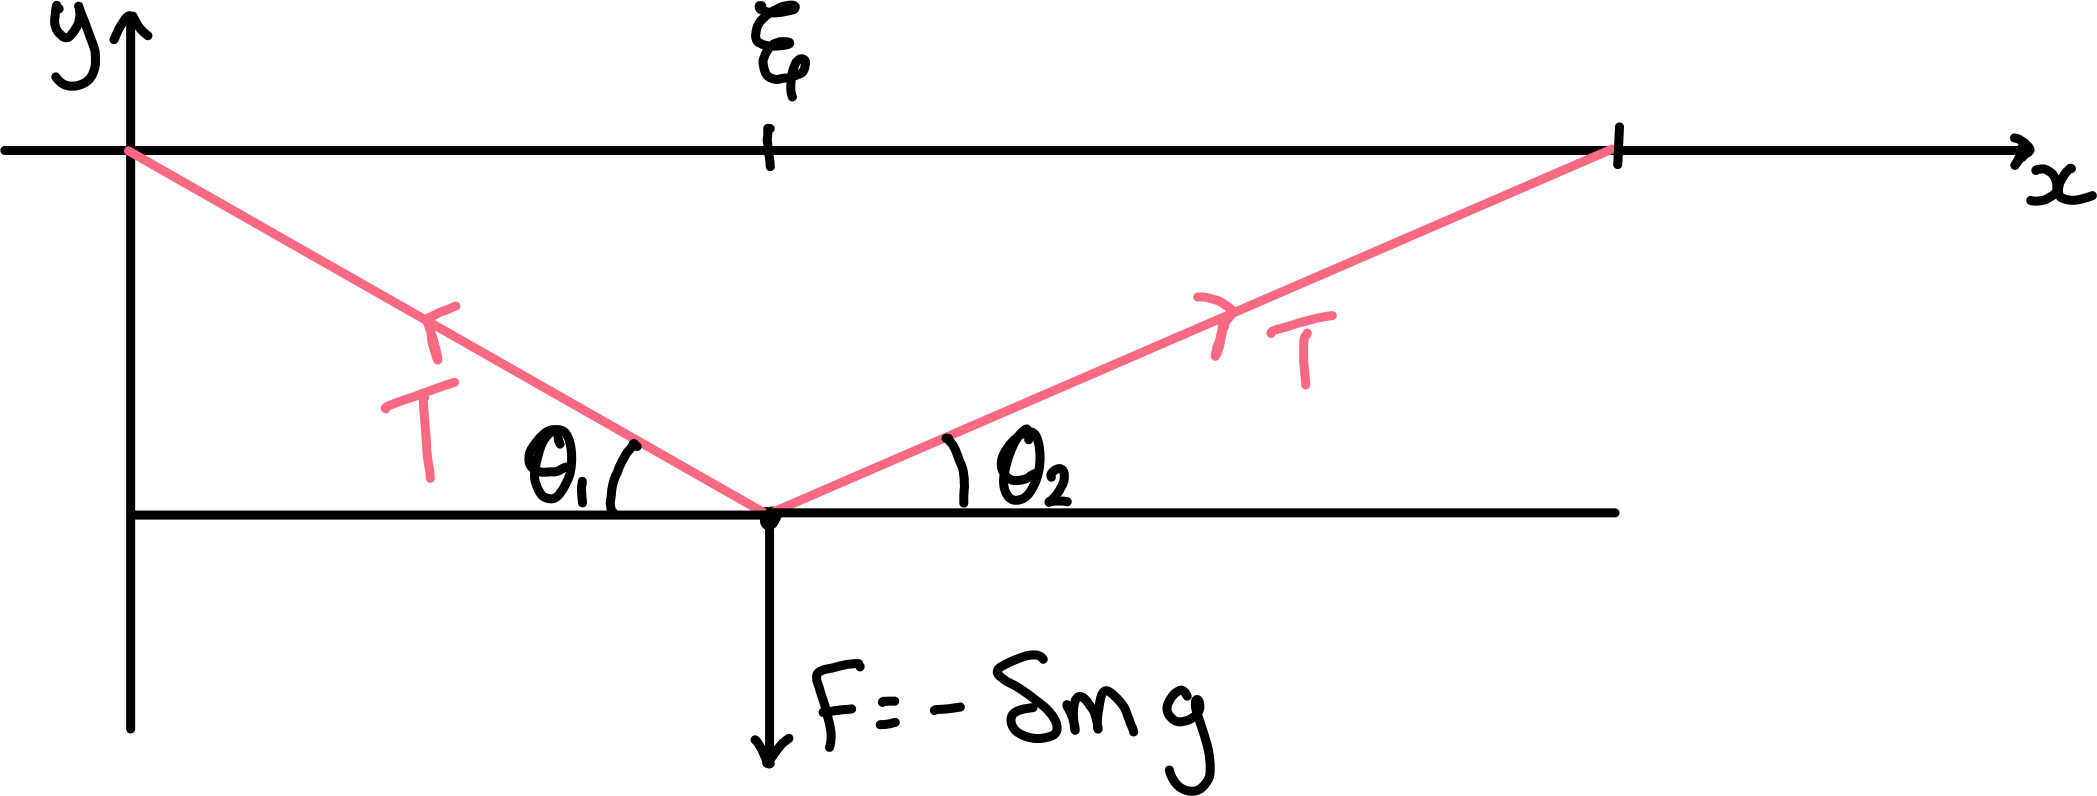
\includegraphics[height=5cm]{07-stringdiagram} 
\end{figure}
Resolving in the $y$ direction to find $y_i(\xi_i)$,
\begin{align*}
	0 & = T (\sin \theta_1 + \sin \theta_2) - \delta m g \\
	& = T\qty(\frac{-y_i}{\xi_i} + \frac{-y_i}{1-\xi_i}) - \delta m g \\
	\therefore -T\qty(y_i(1-\xi_i) + y_i \xi_i) & = \delta m g \xi_i(1-\xi_i) \\
	\therefore y_i(\xi_i) & = \frac{-\delta m g}{T} \xi_i (1-\xi_i)
\end{align*}
So the solution is
\begin{align*}
	y_i(x) = \frac{-\delta m g}{T} \begin{cases}
		x(1-\xi_i)    & x < \xi_i \\
		\xi_i (1 - x) & x > \xi_i
	\end{cases}
\end{align*}
which is the generalised sawtooth.
This can alternatively be written
\begin{align} \label{eq:7.4}
	y_i(x) = f_i(\xi) G(x,\xi)
\end{align}
where $f_i$ is a source term, and $G(x,\xi)$ is the Green's function, the solution for a unit point source.
Since the differential equation is linear, we can sum the solutions for $N$ point masses, giving
\begin{align*}
	y(x) = \sum_{i=1}^N f_i(\xi) G(x, \xi_i)
\end{align*}
Taking a \underline{continuum limit},
\begin{align*}
	f_i(\xi) = \frac{-\delta m g}{T} = \frac{-\mu \delta x g}{T} \equiv f(x) \dd{x} \implies f(x) = \frac{-\mu g}{T}
\end{align*}
which gives ($x \mapsto \xi$)
\begin{align} \label{eq:7.5}
	y(x) = \int_0^1 f(\xi) G(x,\xi) \dd{\xi}
\end{align}
where we are integrating over all source positions.
Substituting the Green's function,
\begin{align*}
	y(x) & = \qty(\frac{-\mu g}{T}) \qty[ \underbracket{\int_0^x \xi(1-x) \dd{\xi}}_{x > \xi} + \underbracket{\int_x^1 x(1-\xi) \dd{\xi}}_{x < \xi}] \\
    &= \qty(\frac{-\mu g}{T}) \qty{ \qty[\frac{\xi^2}{2}(1-x)]_0^x + \qty[x \qty(\xi - \frac{\xi^2}{2})]_x^1 } \\
    &= \qty(\frac{-\mu g}{T}) \qty(\frac{x^2}{2}(1-x) - 0 + \frac{x}{2} - x\qty(x-\frac{x^2}{2}))  \\
    &= \qty(\frac{-\mu g}{T}) \cdot \frac{1}{2}x(1-x)
\end{align*}
So we have found the correct solution in two ways; once by direct integration, and once by superimposing point solutions.
In general, direct integration is not trivial, and Green's functions are useful in this case.

\subsection{Definition of Green's function}
We wish to solve the inhomogeneous ODE \cref{eq:2.21}
\begin{align} \label{eq:7.6}
	\mathcal L y \equiv \alpha(x) y'' + \beta(x) y' + \gamma(x) y = f(x)
\end{align}
on $a \leq x \leq b$, where $\alpha \neq 0$ and $\alpha, \beta, \gamma$ are continuous and bounded, taking homogeneous boundary conditions $y(a) = y(b) = 0$. \\
The Green's function for $\mathcal L$ in this case is defined to be the solution for a unit point source at $x = \xi$.
That is, $G(x,\xi)$ is the function that satisfies the boundary conditions and
\begin{align} \label{eq:7.7}
	\mathcal L G(x,\xi) = \delta(x-\xi)
\end{align}
so $G(a,\xi) = G(b,\xi) = 0$.
Then, by linearity, the general solution is given by
\begin{align} \label{eq:7.8}
	y(x) = \int_a^b f(\xi) G(x,\xi) \dd{\xi}
\end{align}
where $y(x)$ satisfies the homogeneous boundary conditions.
We can verify this by checking
\begin{align*}
	\mathcal L y = \int_a^b \mathcal L_{(x)} G(x,\xi) f(\xi) \dd{\xi} = \int_a^b \delta(x-\xi) f(\xi) \dd{\xi} = f(x)
\end{align*}
So the solution is given by the inverse operator
\begin{align*}
	y = \mathcal L^{-1} f;\quad \mathcal L^{-1} = \int_a^b \dd{\xi} G(x,\xi)
\end{align*}

\subsection{Defining properties (summary)}
The Green's function spits into two parts;
\begin{align} \label{eq:7.9}
	G(x,\xi) = \begin{cases}
		G_1(x,\xi) & a \leq x < \xi \\
		G_2(x,\xi) & \xi < x \leq b
	\end{cases}
\end{align}
\begin{enumerate}
    \item \underline{Hom solns} $G$ solves homogenous equation $\forall \; x \neq \xi$ so 
    \begin{align} \label{eq:7.10}
        \mathcal L G_1 = \mathcal L G_2 = 0
    \end{align} 
    \item \underline{Hom b.c.s} $G$ satisfies the homogeneous boundary conditions, so 
    \begin{align} \label{eq:7.11}
        G_1(a, \xi) = 0,\quad G_2(b, \xi) = 0
    \end{align} 
    \item \underline{Continuity condition} $G$ must be continuous at $x = \xi$, hence
    \begin{align} \label{eq:7.12}
        G_1(\xi, \xi) = G_2(\xi, \xi)
    \end{align} 
    \item \underline{Jump condition} There is a jump condition; the derivative of $G$ is discontinuous at $x = \xi$.
    This satisfies
    \begin{align} \label{eq:7.13}
        [G']_{\xi_-}^{\xi_+} = \eval{\dv{G_2}{x}}_{x = \xi_+} - \eval{\dv{G_1}{x}}_{x = \xi_-} = \frac{1}{\alpha(\xi)}
    \end{align}
    where $\alpha(x)$ is defined in \cref{eq:7.6}.
\end{enumerate} 

\subsection{Explicit form for Green's functions}
We want to solve
\begin{align*}
	\mathcal L G(x,\xi) = \delta(x-\xi)
\end{align*}
on $a \leq x \leq b$, subject to homogeneous boundary conditions $G(a,\xi) = G(b,\xi) = 0$ (with $a < \xi < b$).
The functions $G_1, G_2$ satisfy the homogeneous equation, so $\mathcal L G_i(x,\xi) = 0$.

\subsubsection{1 \& 2, Solve hom eqn with hom b.cs}
Suppose there exist two independent homogeneous solutions $y_1(x), y_2(x)$ to $\mathcal L y = 0$.
Then, $G_1 = A y_1 + B y_2$, such that $A y_1(a) + B y_2(a) = 0$, which gives a constraint between $A$ and $B$.
This defines a complementary function $y_-(x)$ such that $y_-(a) = 0$.
The general homogeneous solution with $G_1(a) = 0$ is
\begin{align} \label{eq:7.14}
	G_1 = C y_-
\end{align}
$C$ will be found later.

Similarly we can define $y_+$ as a linear combination of $y_1, y_2$ such that $y_+(b) = 0$.
\begin{align} \label{eq:7.15}
	G_2 = D y_+
\end{align}

\subsubsection{3. Why is $G$ continuous at $x = \xi$?}
Suppose $G$ was discontinuous at $x = \xi$, so locally $G \propto H(x - \xi) + \dots$ \cref{eq:6.7} which implies $G' \propto \delta(x - \xi)$ and $G'' \propto \delta'(x - \xi)$.
So LHS $\mathcal{L} G \propto \alpha(x) \delta'(x - \xi) + \beta(x) \delta(x - \xi) + \gamma(x) H(x - \xi)$.
But on RHS there is not $\delta'(x - \xi) \neq \delta(x - \xi)$ \Lightning.
Hence, we have $[G]_{\xi_-}^{\xi^+} = 0$, so we require $G_1(\xi, \xi) = G_2(\xi, \xi)$ for continuity, hence
\begin{align} \label{eq:7.16}
	C y_-(\xi) = D y_+(\xi)
\end{align}

\subsubsection{4. Why the jump condition for $G'$ at $x = \xi$}
Integrate $\mathcal{L} G(x, \xi) = \delta(x - \xi)$ across $x = \xi$:
\begin{align*}
	LHS &= \int_{\xi_-}^{\xi^+} \mathcal{L} G \dd{x} \\
	&= \int_{\xi_-}^{\xi^+} \alpha G'' + \beta G' + \gamma G \dd{x}
	\intertext{Integrate by parts}
	&= \underbracket{\alpha(\xi) [G']_{\xi_-}^{\xi^+}}_\text{by cty of $\alpha(x)$} + (\beta - \alpha')[G]_{\xi_-}^{\xi^+} + \int_{\xi_-}^{\xi^+} (\gamma - \beta' + \alpha'') G \dd{x}
\end{align*} 
The latter two terms are $0$ as $\xi^+ \to \xi_-$ by continuity of Green's function \cref{eq:7.12}.
$RHS = \int_{\xi_-}^{\xi^+} \delta(x - \xi) \dd{x} = 1$.

Thus $[G']_{\xi_-}^{\xi^+} = \frac{1}{\alpha(\xi)}$, we have
\begin{align} \label{eq:7.17}
	Dy'_+(\xi) - C y_-'(\xi) = \frac{1}{\alpha(\xi)}
\end{align}
We can solve these equations \cref{eq:7.16,eq:7.17} for $C, D$ simultaneously to find
\begin{align} \label{eq:7.18}
	C(\xi) = \frac{y_+(\xi)}{\alpha(\xi)W(\xi)};\quad D(\xi) = \frac{y_-(\xi)}{\alpha(\xi)W(\xi)}
\end{align}
where $W(\xi)$ is the Wronskian
\begin{align} \label{eq:7.19}
	W(\xi) = y_-(\xi) y_+'(\xi) - y_+(\xi) y_-'(\xi)
\end{align}
which is nonzero if $y_-, y_+$ are linearly independent.
Hence,
\begin{align} \label{eq:7.20}
	G(x,\xi) = \begin{cases}
		\frac{y_-(x) y_+(\xi)}{\alpha(\xi)W(\xi)} & a \leq x \leq \xi \\
		\frac{y_-(\xi) y_+(x)}{\alpha(\xi)W(\xi)} & \xi \leq x \leq b
	\end{cases}
\end{align}

\subsection{Solving boundary value problems}
We know that the solution of $\mathcal L y = f$ \cref{eq:7.6} with $y(a) = y(b) = 0$ is
\begin{align*}
	y(x) = \int_a^b G(x,\xi) f(\xi) \dd{\xi}
\end{align*}
We can split this into two intervals given that $G = G_1$ for $\xi > x$ and $G = G_2$ for $\xi < x$.
\begin{align}
	y(x) & = \int_a^x G_2(x,\xi) f(\xi) \dd{\xi} + \int_x^b G_1(x,\xi) f(\xi) \dd{\xi} \notag \\
    & = y_+(x) \int_a^x \frac{y_-(\xi) f(\xi)}{\alpha(\xi)W(\xi)} \dd{\xi} + y_-(x) \int_a^x \frac{y_+(\xi) f(\xi)}{\alpha(\xi)W(\xi)} \dd{\xi} \label{eq:7.21}
\end{align}

\begin{note}
	\begin{enumerate}
		\item Note that if $\mathcal L$ is in Sturm-Liouville form, so $\beta = \alpha'$, then the denominator $\alpha(\xi)W(\xi)$ is a \underline{constant} and $G$ is \underline{symmetric}; $G(x,\xi) = G(\xi,x)$.
		\begin{exercise}
			Show that $\frac{d }{d x} (\alpha(x) W(x)) = 0$ using $\beta = \alpha'$ and self-adjoint form \cref{eq:2.10} $y_- \mathcal{L} y_+ - y_+ \mathcal{L} y_-$.
		\end{exercise} 
		\item Often, by convention, we take $\alpha = 1$ (however Sturm-Liouville form typically takes $\alpha < 0$).
		\item  Indefinite integrals $\int_x$ in \cref{eq:7.21} are particular integrals in general solution \cref{eq:2.5}.
		\begin{exercise}
			For $-y'' = f(x)$, $y(0) = y(1) = 0$ directly construct the Green's function \cref{eq:7.4}
			\begin{align*}
				G(x, \xi) = \begin{cases}
					x (1 - \xi) & x \leq \xi \\
					\xi (1 - x) & x > \xi
				\end{cases} 
			\end{align*} 
			(i.e. using $y_{hom} = Ax + b$ and $\alpha = -1$).
		\end{exercise} 
	\end{enumerate} 
\end{note} 

\begin{example}
	Consider $y'' - y = f(x)$ with $y(0) = y(1) = 0$.
	Let us construct $G(x, \xi)$.

	\underline{1 \& 2}
	Homogeneous solutions are $y_1 = e^x$, $y_2 = e^{-x}$.
	Imposing boundary conditions (by inspection),
	\begin{align*}
		G = \begin{cases}
			C \sinh x    & 0 \leq x < \xi \\
			D \sinh(1-x) & \xi < x \leq b
		\end{cases}
	\end{align*}

	\underline{3}
	Continuity at $x = \xi$ implies
	\begin{align*}
		C \sinh \xi = D \sinh (1 - \xi) \implies C = D \frac{\sinh (1-\xi)}{\sinh \xi}
	\end{align*}

	\underline{4}
	The jump condition is
	\begin{align*}
		-D \cosh(1-\xi) - C \cosh \xi = 1
	\end{align*}
	Hence,
	\begin{align*}
		-D\qty[\cosh(1-\xi)\sinh \xi + \sinh(1-\xi)\cosh \xi] & = \sinh \xi  \\
		-D\qty[\sinh((1-\xi) + \xi)] &= \sinh \xi \\
		-D\sinh 1 &= \sinh \xi \\
		D &= -\frac{\sinh \xi}{\sinh 1} \\
		\therefore C &= \frac{-\sinh(1-\xi)}{\sinh 1}
	\end{align*}
	So the solution is,
	\begin{align} \label{eq:7.22}
		y(x) = \frac{-\sinh(1-x)}{\sinh 1} \int_0^x \sinh \xi f(\xi) \dd{\xi} - \frac{\sinh x}{\sinh 1} \int_x^1 \sinh (1-\xi) f(\xi) \dd{\xi}
	\end{align}
\end{example}
Suppose we have inhomogeneous boundary conditions.
In this case, we want to find a homogeneous solution $y_p$ that solves the inhomogeneous boundary conditions.
That is, $\mathcal L y_p = 0$ but $y_p(a) \neq 0, y_p(b) \neq 0$ are as required for the inhomogeneous boundary conditions.

Then, by subtracting this solution from the original equation, we can solve using a homogeneous set of boundary conditions.
We can find Green's fcn for $\mathcal{L} y_g = f$ with $y_g(a) = y_g(b) = 0$ where $y_g = y - y_p$.

\begin{example}
	Suppose $y'' - y = f(x)$ with $y(0) = 0, y(1) = 1$. \\
	\begin{align*}
		y_p &= A \sinh x + B \cosh x \\
		y_p(0) &= 0 \implies B = 0 \\
		y_p(1) &= 1 \implies A = \frac{1}{\sinh 1}
	\end{align*} 
	Solve for $y_g = y - y_p$ with $y_g(0) = y_g(1) = 0$.
	Solution $y(x) = \frac{\sinh x}{\sinh 1} + y_g$ (i.e. solution \cref{eq:7.22}).
\end{example}

\subsection{Higher-order ODEs (BVP)}
Suppose $\mathcal L y = f(x)$ where $\mathcal L$ is an $n$th order linear differential operator, and $\alpha(x)$ is the coefficient for the highest degree derivative ($\alpha(x) \frac{d^n y}{d x^n}$).
Suppose that homogeneous boundary conditions are satisfied.
Then we can define the Green's function in this case to be the function that solves
\begin{align*}
	\mathcal L G(x,\xi) = \delta(x-\xi)
\end{align*}
which has the properties:
\begin{enumerate}
	\item $G_1, G_2$ are homogeneous solutions satisfying the homogeneous boundary conditions;
	\item $G_1^{(k)}(\xi) = G_2^{(k)}(\xi)$ for $k \in \qty{0, \dots, n-2}$;
	\item $G_2^{(n-1)}(\xi^+) - G_1^{(n-1)}(\xi^-) = \frac{1}{\alpha(\xi)}$.
\end{enumerate}
See Sheet 3, Q4

\subsection{Eigenfunction expansions of Green's functions}
Suppose $\mathcal L$ is in Sturm-Liouville form with eigenfunctions $y_n(x)$ and eigenvalues $\lambda_n$.
We seek $G(x,\xi) = \sum_{n=1}^\infty A_n y_n(x)$ satisfying $\mathcal L G = \delta(x-\xi)$.
\begin{align*}
	\mathcal L G &= \sum_n A_n \mathcal L y_n \\
	&= \sum_n A_n \lambda_n w(x) y_n(x) \text{ by \cref{eq:2.12}}
\end{align*}
The $\delta$ function has expansion
\begin{align*}
	\delta(x-\xi) = w(x) \sum_n \frac{y_n(\xi) y_n(x)}{N_n} \text{ by \cref{eq:6.15} where } N_n = \int w y_n^2 \dd{x}
\end{align*}
Hence,
\begin{align*}
	A_n(\xi) = \frac{y_n(\xi)}{\lambda_n N_n}
\end{align*}
Thus,
\begin{align}
	G(x,\xi) &= \sum_{n=1}^\infty \frac{y_n(\xi) y_n(x)}{\lambda_n \int w y_n^2 \dd{x}} \label{eq:7.23} \\
	&= \sum_{n=1}^\infty \frac{Y_n(\xi) Y_N(x)}{\lambda_n} \text{ (unit norm)} \notag
\end{align}
which was already obtained earlier in the course when studying Sturm-Liouville theory in \cref{eq:2.31}.

\subsection{Constructing Green's function for an initial value problem}
Suppose we want to solve 
\begin{align} \label{eq:7.24}
	\mathcal L y = f(t) \text{ for } t \geq a \text{ with } y(a) = y'(a) = 0,
\end{align}
using $G(t, \tau)$ satisfying $\mathcal L G = \delta(t - \tau)$ with the same b.cs.

\underline{For $t < \tau$}, we have
\begin{align*}
	G_1 = A y_1(t) + B y_2(t);\quad A y_1(a) + B y_2(a) = 0;\quad A y_1'(a) + B y_2'(a) = 0
\end{align*}
If $A \neq B \neq 0$, then we can solve this by dividing out $A, B$ and find $y_1 y_2' - y_2 y_1' = 0$.
Since the Wronskian at $a$ cannot be zero, $A = B = 0$.
So $G_1(t,\tau) \equiv 0$ for $a \leq t < \tau$, so there is no change until the `impulse' at $t = \tau$.

\underline{For $t > \tau$}, by continuity, \cref{eq:7.12}, we must have $G_2(\tau, \tau) = 0$.
So we choose a complementary function $G_2 = D y_+(t)$ with $y_+(t) = A y_1(t) + B y_2(t)$, and b.c $y_+(\tau) = 0$.
The discontinuity in the derivative, \cref{eq:7.13}, implies that
\begin{align*}
	G_2'(\tau, \tau) - \underbracket{G_1'(\tau, \tau)}_0 = Dy_+'(\tau) = \frac{1}{\alpha(\tau)}
\end{align*}
Hence,
\begin{align*}
	A y_1'(\tau) + B y_2'(\tau) = \frac{1}{\alpha(\tau)} \implies D(\tau) = \frac{1}{\alpha(\tau) y_+'(\tau)}
\end{align*}
or we can find soln for $A, B$ directly.

Hence we have a non-trivial solution
\begin{align} \label{eq:7.25}
	G(t, \tau) = \begin{cases}
		0 & t < \tau \\
		\frac{y_+(t)}{\alpha(\tau) y_+'(\tau)} & t > \tau
	\end{cases}
\end{align}
The initial value problem \cref{eq:7.24} has solution
\begin{align} \label{eq:7.26}
	y(t) = \int_a^t G_2(t, \tau) f(\tau) \dd{\tau} = \int_a^t \frac{y_+(t) f(\tau)}{y_+'(\tau)} \dd{\tau}
\end{align}
Causality is `built in' to this solution.
Only forces which occur before $t$ may have an impact on $y(t)$.
\begin{example}
	Let us solve $y''-y = f(t)$ with $y(0) = y'(0) = 0$.
	The homogeneous solution and initial conditions are
	\begin{align*}
		t < \tau \implies G_1 \equiv 0
	\end{align*}
	and
	\begin{align*}
		t > \tau \implies G_2 = A e^t + Be^{-t}
	\end{align*}
	By continuity $G_2(\tau, \tau) = 0 \implies G_2 = D \sinh (t - \tau)$.
	Now,
	\begin{align*}
		[G']_{\tau_-}^{\tau_+} = \frac{1}{\alpha(\tau)} = 1 \implies G_2'(\tau, \tau) = D \cosh 0 = D = 1
	\end{align*}
	Hence, the solution \cref{eq:7.26} is
	\begin{align*}
		y(t) = \int_0^t f(\tau) \sinh (t - \tau) \dd{\tau}
	\end{align*}
\end{example}
    \section{Fourier Transforms}

\subsection{Definitions}
\begin{definition}[Fourier transform]
	The \vocab{Fourier transform} of a function $f(x)$ is
	\begin{align} \label{eq:8.1}
		\widetilde f(k) = \mathcal F(f)(k) = \int_{-\infty}^\infty f(x) e^{-ikx} \dd{x}
	\end{align}
	The \vocab{inverse Fourier transform} is
	\begin{align} \label{eq:8.2}
		f(x) = \mathcal F\inv\qty(\widetilde f)(x) = \frac{1}{2\pi} \int_{-\infty}^\infty \widetilde f(k) e^{ikx} \dd{k}
	\end{align}
	Different internally-consistent definitions exist, which distribute the multiplicative constants in different ways.
\end{definition}

\begin{theorem}[Fourier inversion theorem]
	For a function $f(x)$,
	\begin{align} \label{eq:8.3}
		\mathcal F\inv (\mathcal F (f))(x) = f(x)
	\end{align}
	with a sufficient condition that $f$ and $\widetilde f$ are \underline{absolutely integrable}, so
	\begin{align*}
		\int_{-\infty}^\infty \abs{f(x)} \dd{x} = M < \infty.
	\end{align*}
	In particular, $f \to 0$ as $x \to \pm \infty$.
\end{theorem}

\begin{example}
	Consider the Gaussian,
	\begin{align} \label{eq:8.4}
		f(x) = \frac{1}{\sigma \sqrt{\pi}} \exp[-\frac{x^2}{\sigma^2}]
	\end{align}
	We wish to compute its Fourier transform.
	Since $i \sin kx$ is an odd function,
	\begin{align*}
		\widetilde f(k) = \frac{1}{\sigma \sqrt{\pi}} \int_{-\infty}^\infty \exp[-\frac{x^2}{\sigma^2}] \exp[-ikx] \dd{x} = \frac{1}{\sigma \sqrt{\pi}} \int_{-\infty}^\infty \exp[-\frac{x^2}{\sigma^2}] \cos(kx) \dd{x}
	\end{align*}
	Consider, using Leibniz' rule,
	\begin{align*}
		\dv{\widetilde f}{k} = \frac{-1}{\sigma \sqrt{\pi}} \int_{-\infty}^\infty x\exp[\frac{-x^2}{\sigma^2}] \sin kx \dd{x}
	\end{align*}
	Integrating by parts,
	\begin{align*}
		\dv{\widetilde f}{k} & = \frac{1}{\sigma \sqrt{\pi}} \underbracket{\qty[\frac{\sigma^2}{2} \exp[\frac{-x^2}{\sigma^2}] \sin kx]_{-\infty}^\infty}_0 - \frac{1}{\sigma \sqrt{\pi}} \int_{-\infty}^\infty \frac{k\sigma^2}{2} \exp[\frac{-x^2}{\sigma^2}] \cos kx \dd{x} \\
        & = -\frac{k\sigma^2}{2} \widetilde f(k)
	\end{align*}
	This is a differential equation for $\widetilde f$, which gives
	\begin{align*}
		\widetilde f(k) = C \exp[-\frac{k^2\sigma^2}{4}]
	\end{align*}
	Suppose $k = 0$.
	Then, in the original expression for the Fourier transform, we can directly find $\widetilde f(0) = 1$.
	Hence $C \exp[-\frac{0^2\sigma^2}{4}] = 1 \implies C = 1$.
	Hence,
	\begin{align} \label{eq:8.5}
		\widetilde f(k) = \exp[-\frac{k^2\sigma^2}{4}]
	\end{align}
	which is another Gaussian with the width parameter inverted.
\end{example}

\begin{exercise}
    Show that $\mathcal{F}\inv(e^{-k^2 \sigma^2 / 4}) = f(x)$ (try completing the square).
\end{exercise} 

\begin{exercise}
    Show that $f(x) = e^{-a |x|}$, $a > 0$, has FT 
    \begin{align} \label{eq:8.6}
        \widetilde{f} = \frac{2a}{a^2 + k^2}
    \end{align} in two ways.
    \begin{enumerate}
        \item Integrate $2 \int_{0}^{\infty} e^{-ax} \cos kx \dd{x}$ by parts twice.
        \item Integrate $\int_{0}^{\infty} e^{-(a - ik) x} \dd{x} + \int_{-\infty}^{0} e^{(a + ik)x} \dd{x}$ directly.
    \end{enumerate} 
    Note that if $f(x) = \begin{cases}
        e^{-ax} & x > 0 \\
        0 & x \leq 0
    \end{cases}$ ($a > 0$) then 
    \addtocounter{equation}{-1}
    \begin{subequations}
        \begin{align} \label{eq:8.6a}
            \widetilde{f}(k) = \frac{1}{ik + a}
        \end{align} 
    \end{subequations}
\end{exercise} 

\subsection{Converting Fourier series into Fourier transforms}
Recall that the complex form of the Fourier series, \cref{eq:1.13}, is
\begin{align*}
	f(x) = \sum_{n=-\infty}^\infty c_n e^{ik_n x}
\end{align*}
where $k_n = \frac{n\pi}{L}$.
We can write in particular $k_n = n \Delta k$ where $\Delta k = \frac{\pi}{L}$.
Then,
\begin{align*}
	c_n = \frac{1}{2L} \int_{-L}^L f(x) e^{-ik_n x} \dd{x} = \frac{\Delta k}{2\pi} \int_{-L}^L f(x) e^{-ik_n x}\dd{x}
\end{align*}
Now, re-substituting into the Fourier series,
\begin{align*}
	f(x) = \sum_{n=-\infty}^\infty \frac{\Delta k}{2\pi} e^{i k_n x} \int_{-L}^L f(x') e^{-ik_n x'} \dd{x'}
\end{align*}
But interpreting the sum multiplied by $\Delta k$ as a Riemann integral,
\addtocounter{equation}{-1}
\begin{subequations}
	\addtocounter{equation}{1}
	\begin{align} \label{eq:8.6b}
		\sum_{n=-\infty}^{\infty} \Delta k g(k_n) \to \int_{-\infty}^{\infty} g(k) \dd{k}
	\end{align} 
\end{subequations}
So,
\begin{align*}
	f(x) \to \int_{-\infty}^\infty \frac{1}{2\pi} e^{i k_n x} \int_{-L}^L f(x') e^{-ik x'} \dd{x'} \dd{k}
\end{align*}
Taking the limit $L \to \infty$,
\begin{align*}
	f(x) = \frac{1}{2\pi} \int_{-\infty}^\infty \dd{k} e^{i k x} \int_{-\infty}^\infty \dd{x'} f(x') e^{-ik_n x'}
\end{align*}
which is the inverse Fourier transform of the Fourier transform of $f$, which gives the Fourier inversion theorem.
Note that when $f(x)$ is discontinuous at $x$, the Fourier transform gives
\begin{align} \label{eq:8.7}
	\mathcal F\inv(\mathcal F(f))(x) = \frac{1}{2}(f(x_-) + f(x_+))
\end{align}
which is analogous to the result for Fourier series.

\subsection{Properties of Fourier series}
Recall the definition of the Fourier transform.
\begin{align*}
	\widetilde f(k) = \int_{-\infty}^\infty f(x) e^{-ikx} \dd{x}
\end{align*}
\begin{proposition}[Linearity]
	The (inverse) Fourier transform is linear.
	\begin{align} \label{eq:8.8}
		h(x) = \lambda f(x) + \mu g(x) \iff \widetilde h(k) = \lambda \widetilde f(k) + \mu \widetilde g(k)
	\end{align}
\end{proposition} 

\begin{proposition}[Translation]
	Translated functions transform to multiplicative factors.
	\begin{align} \label{eq:8.9}
		h(x) = f(x - \lambda) \iff \widetilde h(k) = e^{-i\lambda k} \widetilde f(k)
	\end{align}
\end{proposition} 

\begin{proof}
	This is because
	\begin{align*}
		\widetilde h(k) = \int f(x - \lambda) e^{-ikx} \dd{x} = \int f(y) e^{-ik(y + \lambda)} \dd{y} = e^{-i\lambda k} \widetilde f(k)
	\end{align*}
\end{proof} 

\begin{proposition}[Frequency Shift]
	Frequency shifts transform to translations in frequency space.
	\begin{align} \label{eq:8.10}
		h(x) = e^{i\lambda x}f(x) \implies \widetilde h(k) = \widetilde f(k - \lambda)
	\end{align}
\end{proposition} 

\begin{proposition}[Scaling]
	A scalar multiple applied to the argument transforms into an inverse scalar multiple.
	\begin{align} \label{eq:8.11}
		h(x) = f(\lambda x) \iff \widetilde h(k) = \frac{1}{\abs{\lambda}} \widetilde f\qty(\frac{k}{\lambda})
	\end{align}
\end{proposition} 

\begin{proposition}[Multiplication by $x$]
	Multiplication by $x$ transforms into an imaginary derivative.
	\begin{align} \label{eq:8.12}
		h(x) = xf(x) \iff \widetilde h(k) = i\widetilde f'(k)
	\end{align}
\end{proposition} 

\begin{proof}
	This is because
	\begin{align*}
		\int_{-\infty}^\infty xf(x) e^{-ikx} \dd{x} = \frac{-1}{i} \dv{k} \int_{-\infty}^\infty f(x) e^{-ikx} \dd{x}
	\end{align*}
\end{proof} 

\begin{proposition}[Derivatives]
	Derivatives transform into a multiplication by $ik$.
	\begin{align} \label{eq:8.13}
		h(x) = f'(x) \iff \widetilde h(k) = ik \widetilde f(k)
	\end{align}
\end{proposition} 

\begin{proof}
	This is because we can integrate by parts and find
	\begin{align*}
		\widetilde h(k) = \int_{-\infty}^\infty f'(x) e^{-ikx} \dd{x} = \underbrace{\qty[f(x) e^{-ikx}]_{-\infty}^\infty}_{=0} + ik\int_{-\infty}^\infty f(x) e^{-ikx} \dd{x}
	\end{align*}
\end{proof} 

\begin{proposition}[General duality] ~\vspace*{-1.5\baselineskip}
	\begin{align} \label{eq:8.14}
		g(x) = \widetilde{f}(x) \iff \widetilde{g}(k) = 2 \pi f(-k)
	\end{align} 
\end{proposition} 

\begin{proof}
	Consider \cref{eq:8.2} with mapping $x \mapsto -x$, we get
	\begin{align*}
		f(-x) = \frac{1}{2\pi} \int_{-\infty}^\infty \widetilde f(k) e^{-ikx} \dd{k}.
	\end{align*}
	Now swap $k$ and $x$, treating $\widetilde f$ now as a function in position space
	\begin{align*}
		f(-k) = \frac{1}{2\pi} \int_{-\infty}^\infty \widetilde f(x) e^{-ikx} \dd{x}.
	\end{align*}
	Thus
	\begin{align*}
		g(x) = \widetilde f(x) \iff \widetilde g(k) = 2\pi f(-k)
	\end{align*}
\end{proof} 

\begin{corollary} ~\vspace*{-1.5\baselineskip}
	\begin{align*}
		f(-x) = \frac{1}{2\pi} \mathcal F(\mathcal F(f))(x)
	\end{align*}
	Finally,
	\begin{align*}
		\mathcal F^4(f)(x) = 4\pi^2 f(x)
	\end{align*}
\end{corollary} 

\begin{exercise}
	Verify these properties.
\end{exercise} 

\begin{example}
	Consider a function defined by
	\begin{align*}
		f(x) = \begin{cases}
			1 & \abs{x} \leq a   \\
			0 & \text{otherwise}
		\end{cases}
	\end{align*}
	for some $a > 0$.
	By the definition of the Fourier transform,
	\begin{align} \label{eq:8.15}
		\widetilde f(k) = \int_{-\infty}^\infty f(x) e^{-ikx} \dd{x} = \int_{-a}^a e^{-ikx} \dd{x} = \int_{-a}^a \cos kx \dd{x} = \frac{2}{k} \sin ka
	\end{align}
	By the Fourier inversion theorem,
	\begin{align*}
		\frac{1}{\pi} \int_{-\infty}^\infty e^{ikx} \frac{1}{k} \sin ka \dd{k} = f(x)
	\end{align*}
	for $x \neq a$. \\
	Now, in this expression, let $x = 0$ and let $k \mapsto x$.
	We arrive at the \underline{Dirichlet discontinuous formula}.
	\begin{align} \label{eq:8.16}
		\int_0^\infty \frac{\sin ax}{x} \dd{x} = \frac{\pi}{2} \sgn a = \begin{cases}
			\frac{\pi}{2}  & a > 0 \\
			0              & a = 0 \\
			-\frac{\pi}{2} & a < 0
		\end{cases}
	\end{align}
	Here, we allow $a < 0$, so $\sin(-ax) = -\sin ax$.
\end{example}

\subsection{Convolution theorem}
We want to multiply Fourier transforms in the frequency domain (transformed space).
This is useful for filtering or processing signals.
\begin{align*}
	\widetilde h(k) = \widetilde f(k) \widetilde g(k)
\end{align*}
Consider the inverse.
\begin{align}
	h(x) &= \frac{1}{2\pi} \int_{-\infty}^\infty \widetilde f(k) \widetilde g(k) e^{ikx} \dd{k} \notag \\
	&= \frac{1}{2\pi} \int_{-\infty}^\infty \qty(\int_{-\infty}^\infty f(y) e^{-iky} \dd{y}) \widetilde g(k) e^{ikx} \dd{k} \notag \\
	&= \int_{-\infty}^\infty f(y) \qty( \frac{1}{2\pi} \int_{-\infty}^\infty e^{-iky} \widetilde g(k) e^{ikx} \dd{k} ) \dd{y} \notag \\
	&= \int_{-\infty}^\infty f(y) \qty( \frac{1}{2\pi} \int_{-\infty}^\infty \widetilde g(k) e^{ik(x-y)} \dd{k} ) \dd{y} \notag \\
	&= \int_{-\infty}^\infty f(y) g(x-y) \dd{y} \text{ by \cref{eq:8.9}} \notag \\
	&\equiv (f \ast g)(x) \label{eq:8.17}
\end{align}
where $f \ast g$ is called the \textit{convolution} of $f$ and $g$.
By duality \cref{eq:8.14}, we also have
\begin{align} \label{eq:8.18}
	h(x) = f(x) g(x) \iff \widetilde h(k) = \frac{1}{2\pi} \int_{-\infty}^\infty \widetilde f(p) \widetilde g(k-p) \dd{p} = \frac{1}{2\pi}\qty(\widetilde f \ast \widetilde g)(k)
\end{align}

\subsection{Parseval's theorem}
Consider $h(x) = g^\star(-x)$.
\begin{align*}
	\widetilde h(k) & = \int_{-\infty}^\infty g^\star(-x) e^{-ikx} \dd{x} \\
	& = \qty[\int_{-\infty}^\infty g(-x) e^{ikx} \dd{x}]^\star
	\intertext{Let $-x \mapsto y$}
	& = \qty[\int_{-\infty}^\infty g(y) e^{-iky} \dd{y}]^\star \\
	& = \widetilde g^\star(k)
\end{align*}
Substituting this into the convolution theorem \cref{eq:8.17}, with $g(x) \mapsto g^\star(-x)$, we have (RHS is the inverse Fourier transform)
\begin{align*}
	\int_{-\infty}^\infty f(y) g^\star(y-x) \dd{y} = \frac{1}{2\pi} \int_{-\infty}^\infty \widetilde f(k) \widetilde g^\star(k) e^{ikx} \dd{x}
\end{align*}
Taking $x = 0$ in this expression and mapping $y \mapsto x$, we find
\begin{align} \label{eq:8.19}
	\int_{-\infty}^\infty f(x) g^\star(x) \dd{x} = \frac{1}{2\pi} \int_{-\infty}^\infty \widetilde f(k) \widetilde g^\star(k) \dd{x}
\end{align}
Equivalently,
\begin{align} \label{eq:8.20}
	\inner{g,f} = \frac{1}{2\pi} \inner{\widetilde g, \widetilde f}
\end{align}
So the inner product is conserved under the Fourier transform (up to a factor of $2 \pi$).
Now, by setting $g^\star = f^\star$, we have
\begin{align*}
	\int_{-\infty}^\infty \abs{f(x)}^2 \dd{x} = \frac{1}{2\pi} \int_{-\infty}^\infty \abs{\widetilde f(k)}^2 \dd{k}
\end{align*}
This is Parseval's theorem.

\subsection{Fourier transforms of generalised functions}
We can apply Fourier transforms to generalised functions by considering limiting distributions.
Consider the inversion
\begin{align*}
	f(x) & = \mathcal F\inv(\mathcal F(f))(x) \\
	     & = \frac{1}{2\pi} \int_{-\infty}^\infty \qty[\int_{-\infty}^\infty f(u) e^{-iku} \dd{u}] e^{ikx} \dd{k} \\
	     & = \int_{-\infty}^\infty f(u) \underbrace{\qty[\frac{1}{2\pi} \int_{-\infty}^\infty e^{-ik(x-u)} \dd{k}]}_{\delta(x-u)} \dd{u}
\end{align*}
In order to reconstruct $f(x)$ on the right hand side for any function $f$, we must have that the bracketed term is $\delta(x-u)$.
So we identify
\begin{align*}
	\delta(x-u) = \frac{1}{2\pi} \int_{-\infty}^\infty e^{ik(x-u)} \dd{k}
\end{align*}
\begin{itemize}
	\item If $f(x) = \delta(x)$,
	\begin{align} \label{eq:8.21}
		\widetilde f(k) = \int_{-\infty}^\infty \delta(x) e^{ikx} \dd{x} = 1
	\end{align}
	This can be thought of as the Fourier transform of an infinitely thin Gaussian, which becomes an infinitely wide Gaussian (a constant).
	\item If $f(x) = 1$, then
	\begin{align} \label{eq:8.22}
		\widetilde f(k) = \int_{-\infty}^\infty e^{-ikx}\dd{x} = 2\pi \delta(k)
	\end{align}
	This can also be found by the duality formula \cref{eq:8.14}.
	\item If $f(x) = \delta(x - a)$, using \cref{eq:8.9} we have
	\begin{align} \label{eq:8.23}
		\widetilde f(k) = e^{-ika}
	\end{align}
	This is a translation of the original Fourier transform for the $\delta$ function above.
\end{itemize} 

\subsection{Trigonometric functions}
Let $f(x) = \cos \omega x = \frac{1}{2} \qty(e^{i\omega x} + e^{-i \omega x})$.
Then,
\begin{align} \label{eq:8.24}
	\widetilde f(k) = \pi\qty(\delta(k+\omega) + \delta(k-\omega))
\end{align}
For $f(x) = \sin \omega x$, we have
\begin{align*}
	\widetilde f(k) = i\pi\qty(\delta(k+\omega) - \delta(k-\omega))
\end{align*}
Using duality \cref{eq:8.14},
\begin{align*}
	f(x) & = \frac{1}{2}\qty(\delta(x+a) + \delta(x-a)) \implies \widetilde f(k) = \cos ka  \\
	f(x) & = \frac{1}{2i}\qty(\delta(x+a) - \delta(x-a)) \implies \widetilde f(k) = \sin ka
\end{align*}

\subsection{Heaviside functions}
Let $H(x)$ be the Heaviside function, such that $H(0) = \frac{1}{2}$.
Then, $H(x) + H(-x) = 1$ for all $x$ and is cts at $x = 0$.
We can take the Fourier transform of this and find by \cref{eq:8.22}
\begin{align*}
	\widetilde H(k) + \widetilde H(-k) = 2\pi \delta(k) \tag{$\ast$}
\end{align*}
Recall that $H'(x) = \delta(x)$, \cref{eq:6.7}.
Thus by \cref{eq:8.13,eq:8.21},
\begin{align*}
	ik \widetilde H(x) = \widetilde \delta(k) = 1 \tag{$\dagger$}
\end{align*}
Since $k \delta(k) = 0$, the two equations for $\widetilde H$ can be consistent if we take
\begin{align} \label{eq:8.25}
	\widetilde H(k) = \pi\delta(k) + \frac{1}{ik}
\end{align}

\subsection{Dirichlet discontinuous formula}
Recall the Dirichlet discontinuous formula \cref{eq:8.16}:
\begin{align*}
	\int_0^\infty \frac{\sin ax}{x} \dd{x} = \frac{\pi}{2} \sgn a = \begin{cases}
		\frac{\pi}{2}  & a > 0 \\
		0              & a = 0 \\
		-\frac{\pi}{2} & a < 0
	\end{cases}
\end{align*}
We can rewrite this as
\begin{align*}
	\frac{1}{2} \sgn x = \frac{1}{2\pi} \int_{-\infty}^\infty \frac{e^{ikx}}{ik} \dd{k}
\end{align*}
since the cosine term divided by $ik$ is odd.
Hence,
\begin{align} \label{eq:8.26}
	f(x) = \frac{1}{2} \sgn x \iff \widetilde f(k) = \frac{1}{ik}
\end{align}
This is the preferred form for a Heaviside-type function when used in Fourier transforms.

\subsection{Solving ODEs for boundary value problems}
Consider $y'' - y = f(x)$ with homogeneous boundary conditions $y \to 0$ as $x \to \pm \infty$.
Taking the Fourier transform of this expression, we find by \cref{eq:8.13}
\begin{align*}
	(-k^2 - 1) \widetilde y = \widetilde f
\end{align*}
Thus, the solution is
\begin{align*}
	\widetilde y(k) = \frac{-\widetilde f(k)}{1+k^2} \equiv \widetilde f(k) \widetilde g(k)
\end{align*}
where $\widetilde g(k) = \frac{-1}{1 + k^2}$.
Note that $\widetilde g(k)$ is the Fourier transform of $g(x) = -\frac{1}{2} e^{-\abs{x}}$, \cref{eq:8.6}.
Applying the convolution theorem \cref{eq:8.17},
\begin{align*}
	y(x) &= \int_{-\infty}^\infty f(u) g(x-u) \dd{u} \\
	     &= -\frac{1}{2} \int_{-\infty}^\infty f(u) e^{-\abs{x-u}}\dd{u} \\
	     &= -\frac{1}{2} \qty[ \int_{-\infty}^x f(u) e^{u-x}\dd{u} + \int_x^\infty f(u) e^{x-u}\dd{u} ]
\end{align*}
This is in the form of a boundary value problem Green's function \cref{eq:7.20}.
We can construct the same results by constructing the Green's function directly or by using inverse fourier transform on $\widetilde y(k)$.

\subsection{Signal processing}
Suppose we have an input signal $\mathcal I(t)$, which is acted on by some linear operator $\mathcal L_{\text{in}}$ to yield an output $\mathcal O(t)$.
The Fourier transform of the input $\widetilde{\mathcal I}(\omega)$ is called the \vocab{resolution}.
\begin{align} \label{eq:8.27}
	\widetilde{\mathcal I}(\omega) = \int_{-\infty}^\infty \mathcal I(t) e^{-i\omega t} \dd{t}
\end{align}
In the frequency domain, the action of $\mathcal L_{\text{in}}$ on $\mathcal I(t)$ means that $\widetilde{\mathcal I}(\omega)$ is multiplied by a \vocab{transfer function} $\widetilde{\mathcal R}(\omega)$ to yield outupt,
\begin{align} \label{eq:8.28}
	\mathcal O(t) = \frac{1}{2\pi} \int_{-\infty}^\infty \widetilde{\mathcal R}(\omega) \widetilde{\mathcal I}(\omega) e^{i\omega t} \dd{\omega}
\end{align}
The inverse Fourier transform of the transfer function, $\mathcal R$, is called the \vocab{response function}, which is given by
\begin{align} \label{eq:8.29}
	\mathcal R(t) = \frac{1}{2\pi} \int_{-\infty}^\infty \widetilde{\mathcal R}(\omega) e^{i \omega t}\dd{\omega}
\end{align}
By the convolution theorem,
\begin{align*}
	\mathcal O(t) = \int_{-\infty}^\infty \mathcal I(u) \mathcal R(t-u) \dd{u}
\end{align*}
Suppose there is no input ($\mathcal I(t) = 0$) for $t < 0$.
By causality, there should be zero output for the response function ($\mathcal R(t) = 0$) for $t < 0$.
Therefore, we require $0 < u < t$ and hence
\begin{align} \label{eq:8.30}
	\mathcal O(t) = \int_0^t \mathcal I(u) \mathcal R(t-u) \dd{u}
\end{align}
which resembles an initial value problem Green's function \cref{eq:7.26}.

\subsection{General transfer functions for ODEs}
Suppose an input-output relationship is given by a linear ODE (nth order).
\begin{align} \label{eq:8.31}
	\mathcal L \mathcal O(t) \equiv \qty(\sum_{i=0}^n a_i \dv[i]{x}) \mathcal O(t) \equiv \mathcal I(t)
\end{align}
Here, $\mathcal L_{\text{in}} = 1$.
We want to solve this ODE using a Fourier transform.
\begin{align*}
	(a_0 + a_1 i\omega - a_2 \omega^2 - a_3 i\omega^3 + \dots + a_n (i \omega)^n) \widetilde{\mathcal O}(\omega) = \widetilde{\mathcal I}(\omega)
\end{align*}
We can solve this algebraically in Fourier transform space.
The transfer function is
\begin{align} \label{eq:8.32}
	\widetilde{\mathcal R}(\omega) = \frac{1}{a_0 + \dots + a_n (i \omega)^n}
\end{align}
We factorise the denominator to find partial fractions.
Suppose there are $J$ distinct roots $(i \omega - c_j)^{k_j}$, where $k_j$ is the algebraic multiplicity of the $j$th root, so $\sum_{j=1}^J k_j = n$.
So we can write
\begin{align*}
	\widetilde{\mathcal R}(\omega) = \frac{1}{(i \omega - c_1)^{k_1} \dots (i \omega - c_J)^{k_J}}
\end{align*}
Expressing this as partial fractions,
\begin{align} \label{eq:8.33}
	\widetilde{\mathcal R}(\omega) = \sum_{j=1}^J \sum_{m=1}^{k_i} \frac{\Gamma_{jm}}{(i\omega - c_j)^m}
\end{align}
The $\Gamma_{jm}$ terms are constant.
To solve this, we must find the inverse Fourier transform of $(i\omega - a)^{-m}$.
Recall that \cref{eq:8.6a}
\begin{align*}
	\mathcal F\inv\qty(\frac{1}{i\omega - a}) = \begin{cases}
		e^{at} & t > 0 \\
		0      & t < 0
	\end{cases}
\end{align*}
for $\Re a < 0$.
So we will require $\Re c_j < 0$ for all $j$ to eliminate exponentially growing solutions.
Note that for $m = 2$,
\begin{align*}
	i \dv{\omega} \qty(\frac{1}{i \omega - a}) = \frac{1}{(i \omega - a)^2}
\end{align*}
and recall \cref{eq:8.12}
\begin{align*}
	\mathcal F (t f(t)) = i \mathcal F'(\omega)
\end{align*}
Hence,
\begin{align*}
	\mathcal F\inv\qty(\frac{1}{(i \omega - a)^2}) = \begin{cases}
		t e^{at} & t > 0 \\
		0        & t < 0
	\end{cases}
\end{align*}
Inductively, we arrive at
\begin{align} \label{eq:8.34}
	\mathcal F\inv\qty(\frac{1}{(i \omega - a)^m}) = \begin{cases}
		\frac{t^{m-1}}{(m-1)!} e^{at} & t > 0 \\
		0                             & t < 0
	\end{cases}
\end{align}
We can therefore invert any transfer function to obtain the response function.
Thus the response function takes the form
\begin{align} \label{eq:8.35}
	\mathcal R(t) = \sum_{j=1}^J \sum_{m=1}^{k_i} \Gamma_{jm} \frac{t^{m-1}}{(m-1)!} e^{c_j t},\quad t > 0
\end{align}
and zero for $t < 0$.
We can now solve such differential equations, \cref{eq:8.31}, in Green's function form \cref{eq:8.30}, or directly invert $\widetilde{\mathcal R}(\omega) \widetilde{\mathcal I}(\omega)$ for a polynomial $\widetilde{\mathcal I}(\omega)$.

\subsection{Damped oscillator}
We can use the Fourier transform method to solve the differential equation
\begin{align*}
	\mathcal L y \equiv y'' + 2py' + (p^2 + q^2)y = f(t)
\end{align*}
where $p > 0$.
Consider homogeneous boundary conditions $y(0) = y'(0) = 0$.
The Fourier transform is
\begin{align*}
	(i\omega)^2 \widetilde y + 2 i p \omega \widetilde y + (p^2 + q^2) \widetilde y = \widetilde f
\end{align*}
Hence,
\begin{align*}
	\widetilde y = \frac{\widetilde f}{-\omega^2 + 2ip\omega + p^2 + q^2} \equiv \widetilde R \widetilde f
\end{align*}
We can invert this using the convolution theorem by inverting $\widetilde R$.
\begin{align*}
	y(t) = \int_0^t \mathcal R(t-\tau) f(\tau) \dd{\tau}
\end{align*}
where the response function is
\begin{align*}
	\mathcal R(t - \tau) = \frac{1}{2\pi} \int_{-\infty}^\infty \frac{e^{i\omega(t-\tau)}}{p^2 + q^2 + 2ip\omega - \omega^2} \dd{\omega}
\end{align*}
We can show that $\mathcal L \mathcal R(t-\tau) = \delta(t-\tau)$ using \cref{eq:8.23}; in other words, $\mathcal R$ is the Green's function (Sheet 3, Q4).

\subsection{Discrete sampling and the Nyquist frequency}
Suppose a signal $h(t)$ is sampled at equal times $t_n = n\Delta$ with a time step $\Delta$ and values
\begin{align} \label{eq:8.36}
	h_n = h(t_n) = h(n\Delta),\quad n \in \mathbb{Z}
\end{align}
The sampling frequency is therefore $\Delta\inv$, so the sampling angular velocity is $\omega_s = 2\pi f_s = \frac{2\pi}{\Delta}$.

\begin{definition}[Nyquist Frequency]
	The \vocab{Nyquist frequency} is the highest frequency actually sampled at $\Delta$,
	\begin{align} \label{eq:8.37}
		f_c = \frac{1}{2 \Delta}
	\end{align} 
\end{definition} 

Suppose we have a signal $g_f$ with a given frequency $f$.
We will write
\begin{align} \label{eq:8.38}
	g_f(t) = A \cos(2\pi f t + \phi) = \Re \qty(A e^{2 \pi i f t + \phi}) = \frac{1}{2} \qty(A e^{2 \pi i f t + \phi}) + \frac{1}{2} \qty(A e^{-2 \pi i f t + \phi})
\end{align}
where $A \in \mathbb R$.
Note that this signal has two `frequencies'; a positive and a negative frequency.
The combination of these frequencies gives the full wave.

Suppose we sample $g_f(t)$ at the Nyquist frequency, so $f = f_c$.
Then,
\begin{align}
	g_{f_c}(t_n) & = A \cos(2 \pi \frac{1}{2\Delta} n \Delta + \phi) \notag \\
	& = A \cos(\pi n + \phi) \notag \\
	& = A \cos \pi n \cos \phi + A \sin \pi n \sin \phi \notag \\
	& = A' \cos(2\pi f_c t_n) \label{eq:8.39}
\end{align}
where $A' = A \cos \phi$.
This has removed half of the information about the wave; the amplitude and the phase have become degenerate.
We have lost phase/amplitude information, there is no longer any distinction between them.
We can identify $f_c$ with $-f_c$ when considering the remaining information; we say that the two frequencies are \textit{aliased} together.

Now, suppose we sample at greater than the Nyquist frequency, in particular $f = f_c + \delta f > f_c$, where for simplicity we let $\delta f < f_c$.
As an exercise, show that
\begin{align}
	g_f(t_n) &= A \cos(2\pi (f_c + \delta f)t_n + \phi) \notag \\
	&= A \cos(2\pi (f_c - \delta f)t_n - \phi) \label{eq:8.40}
\end{align}
So frequencies above the Nyquist frequency are reinterpreted after the sampling as a frequency lower than the Nyquist frequency.
This aliases $f_c + \delta f$ with $f_c - \delta f$.

\subsection{Nyquist-Shannon sampling theorem}
\begin{definition}[Bandwith-Limited]
	A signal $g(t)$ is \vocab{bandwidth-limited} if it contains no frequencies above $\omega_{\max} = 2\pi f_{\max}$.
	In other words, $\widetilde g(\omega) = 0$ for all $\abs{\omega} > \omega_{\max}$.
	In this case,
	\begin{align} \label{eq:8.41}
		g(t) = \frac{1}{2\pi} \int_{-\infty}^\infty \widetilde g(\omega) e^{i\omega t} \dd{\omega} = \frac{1}{2\pi} \int_{-\omega_{\max}}^{\omega_{\max}} \widetilde g(\omega) e^{i\omega t} \dd{\omega}
	\end{align}
\end{definition}

Suppose we set the sampling rate to the Nyquist frequency, so $\Delta = \frac{1}{2f_{\max}}$.
Then,
\begin{align*}
	g_n \equiv g(t_n) = \frac{1}{2\pi} \int_{-\omega_{\max}}^{\omega_{\max}} \widetilde g(\omega) e^{i\pi n \omega / \omega_{\max}} \dd{\omega}
\end{align*}
This is a complex Fourier series coefficient \cref{eq:1.13} $c_n$, multiplied by $\frac{\omega_{\max}}{\pi}$.
The Fourier series is periodic in $\omega$ with period $2 \omega_{\max}$, not in space or time.
\begin{align} \label{eq:8.42}
	\widetilde g_\mathrm{per}(\omega) = \frac{\pi}{\omega_{\max}} \sum_{n=-\infty}^\infty g_n e^{-i \pi n \omega / \omega_{\max}}
\end{align}
The actual Fourier transform $\widetilde g$ is found by multiplying by a top hat window function
\begin{align*}
	\widetilde h(\omega) = \begin{cases}
		1 & \abs{\omega} \leq \omega_{\max} \\
		0 & \text{otherwise}
	\end{cases}
\end{align*}
Hence,
\begin{align} \label{eq:8.4f}
	\widetilde g(\omega) = \widetilde g_\mathrm{per}(\omega) \widetilde h(\omega)
\end{align}
Note that this relation is exact.
Inverting this expression,
\begin{align*}
	g(t) & = \frac{1}{2\pi} \int_{-\infty}^\infty \widetilde g_\mathrm{per}(\omega) \widetilde h(\omega) e^{i \omega t} \dd{\omega} \\
	& = \frac{1}{2\omega_{\max}} \sum_{n=-\infty}^\infty g_n \int_{-\omega_{\max}}^{\omega_{\max}} \exp(i \omega\qty(t - \frac{n \pi}{\omega_{\max}})) \dd{\omega}
\end{align*}
Only the cosine term is even, hence
\begin{align} \label{eq:8.44}
	g(t) = \frac{1}{2\omega_{\max}} \sum_{n=-\infty}^\infty g_n \frac{\sin(\omega_{\max} t - \pi n)}{\omega_{\max} t - \pi n}
\end{align}
Hence, $g(t)$ can be written \textit{exactly} as a combination of countably many discrete sample points.

\subsection{Discrete Fourier transform}
Suppose we have a finite number of samples 
\begin{align} \label{eq:8.45}
	h_m = h(t_m) \text{ for } t_m = m \Delta, \text{ where } m = 0,\dots, N-1
\end{align}
We will approximate the Fourier transform for $N$ frequencies within the Nyquist frequency $f_c = \frac{1}{2\Delta}$, using equally-spaced frequencies, given by $\Delta_f = \frac{1}{N\Delta}$ in the range $-f_c \leq f \leq f_c$.
We could take the convention $f_n = n \Delta_f = \frac{n}{N\Delta}$ for $n = -\frac{N}{2}, \dots, \frac{N}{2}$.
However, this overcounts the Nyquist frequency (which is aliased, \cref{eq:8.39}), giving $N + 1$ frequencies instead of the desired $N$.
Since frequencies above the Nyquist frequency are aliased to below it, \cref{eq:8.40}:
\begin{align*}
	\qty(\frac{N}{2} + m) \Delta f = f_c + \delta f \mapsto \qty(\frac{N}{2} - m)\Delta f = -(f_c - \delta f)
\end{align*}
we can instead use the convention $f_n = n \Delta_f = \frac{n}{N\Delta}$ for
\begin{align} \label{eq:8.46}
	n = 0, \dots, N - 1
\end{align} 
This counts the Nyquist frequency only once.

The \vocab{discrete FT} at a frequency $f_n$ becomes
\begin{align}
	\widetilde h(f_n) & = \int_{-\infty}^\infty h(t) e^{-2\pi if_n t} \dd{t} \notag \\
	& \approx \Delta \sum_{m=0}^{N-1} h_m e^{-2\pi i f_n t_m} \notag \\
	& = \Delta \sum_{m=0}^{N-1} h_m e^{-2\pi i m n / N} \notag \\
	& = \Delta \widetilde h_d(f_n) \label{eq:8.47}
\end{align}
where the function $\widetilde h_d(f_n)$ is the discrete Fourier transform.

The matrix 
\begin{align} \label{eq:8.48}
	[\mathrm{DFT}]_{mn} = e^{-2\pi i m n / N},\ m, n = 0, 1, \dots, N-1
\end{align} defines the discrete Fourier transform for the vector $h = \qty{h_m}$.
The discrete Fourier transform is then
\begin{align*}
	\widetilde h_d = [\mathrm{DFT}] h
\end{align*}
By inverting the discrete Fourier transform matrix, we find
\begin{align*}
	h = [\mathrm{DFT}]\inv \widetilde h_d = \frac{1}{N} [\mathrm{DFT}]^\dagger \widetilde h_d
\end{align*}
since the inverse of the discrete Fourier transform matrix is its adjoint.
The matrix is built from roots of unity $\omega = e^{-2\pi i/N}$.
So, for instance, $n = 4$ gives $\omega = e^{-2\pi i/4} = -i$ giving
\begin{align*}
	[\mathrm{DFT}] = \begin{pmatrix}
		1 & 1  & 1  & 1  \\
		1 & -i & -1 & i  \\
		1 & -1 & 1  & -1 \\
		1 & i  & -1 & -i
	\end{pmatrix}
\end{align*}
The inverse discrete Fourier transform is
\begin{align*}
	h_m &= h(t_m) \\
	    &= \frac{1}{2\pi} \int_{-\infty}^\infty \widetilde h(\omega) e^{i \omega t_m} \dd{\omega} \\
	    &= \int_{-\infty}^\infty \widetilde h(f) e^{2\pi i f t_m} \dd{f} \\
	    &\approx \frac{1}{\Delta N} \sum_{n=0}^{N-1} \Delta \widetilde h_d(f_n) e^{2\pi i m n / N} \\
	    &= \frac{1}{N} \sum_{n=0}^{N-1} \widetilde h_n e^{2\pi i m n / N}
\end{align*}
Hence, we can interpolate the initial function from its samples.
\begin{align*}
	h(t) = \frac{1}{N} \sum_{n=0}^{N-1} \widetilde h_n e^{2\pi i n t / N}
\end{align*}
Parseval's theorem becomes,
\begin{align} \label{eq:8.49}
	\sum_{m=0}^{N-1} \abs{h_m}^2 = \frac{1}{N} \sum_{n=0}^{N-1} \abs{\widetilde h_n}^2
\end{align}
\begin{exercise}
	Prove this.
\end{exercise} 
The convolution theorem for $g_m, h_m$ is
\begin{align} \label{eq:8.50}
	c_k = \sum_{m=0}^{N-1} g_m h_{k-m} \iff \widetilde c_k = \widetilde g_k \widetilde h_k
\end{align}

\subsection{Fast Fourier transform (non-examinable)}
While the discrete Fourier transform is an order $O(N^2)$ operation, we can reduce this into an order $O(n \log N)$ operation.
Such a simplification is called the \vocab{fast Fourier transform}.
We can split the discrete Fourier transform into even and odd parts, noting that $\omega_N = e^{-2\pi i / N}$ implies $\omega_N^2 = e^{-2 \pi i / (N/2)} = \omega_{N/2}$
\begin{align*}
	\widetilde h_k & = \sum_{n=0}^{N-1} h_n \omega_N^{nk}                                                                           \\
    & = \sum_{m=0}^{N/2-1} h_{2m} \omega_N^{2mk} + \sum_{m=0}^{N/2-1} h_{2m + 1} \omega_N^{(2m+1)k}                  \\
    & = \sum_{m=0}^{N/2-1} h_{2m} (\omega_N^2)^{mk} + \omega_N^k \sum_{m=0}^{N/2-1} h_{2m + 1} (\omega_N^2)^{mk}     \\
    & = \sum_{m=0}^{N/2-1} h_{2m} (\omega_{N/2})^{mk} + \omega_N^k \sum_{m=0}^{N/2-1} h_{2m + 1} (\omega_{N/2})^{mk} \\
\end{align*}
This algorithm iteratively reduces the Fourier transform's complexity by a factor of two, until the trivial case of finding the discrete Fourier transform of two data points.

    \part{Inhomogenous ODEs and Greens Functions}
\end{document}